
%\documentclass[11pt,a4paper,pdftex,headexclude,smallheadings,pointlessnumbers,bibtotoc,idxtotoc,twoside,authordate1-4]{article}
%\documentclass[11pt,a4paper,pdftex,headexclude,smallheadings,pointlessnumbers,bibtotoc,idxtotoc,twoside,authordate1-4]{report}

%\documentclass[11pt,a4paper,pdftex,twoside]{book}


%To compile: execute in texworks with the option pdfLatexmakeindex+bibtex

\documentclass[
		twoside,openright,titlepage,numbers=noenddot,manychapters,
		headinclude,%1headlines,
                footinclude=false,cleardoublepage=empty,
                BCOR=5mm,
		fontsize=11pt, % Binding correction, paper type and font size
		%fontsize=10pt,
               % ngerman,american, % Languages
                 enabledeprecatedfontcommands]{scrreprt} 
                
%from lightningsource:
\paperheight = 234mm
\paperwidth = 156mm
%\paperheight = 280mm
%\paperwidth = 216mm




% Includes the file which contains all the document configurations and packages - make sure to edit this file
%%%%%%%%%%%%%%%%%%%%%%%%%%%%%%%%%%%%%%%%%
% Thesis Configuration File
%
% The main lines to change in this file are in the DOCUMENT VARIABLES
% section, the rest of the file is for advanced configuration.
%
%%%%%%%%%%%%%%%%%%%%%%%%%%%%%%%%%%%%%%%%%

%----------------------------------------------------------------------------------------
%	DOCUMENT VARIABLES
%	Fill in the lines below to enter your information into the thesis template
%	Each of the commands can be cited anywhere in the thesis
%----------------------------------------------------------------------------------------

% Remove drafting to get rid of the '[ Date - classicthesis version 4.0 ]' text at the bottom of every page
%\PassOptionsToPackage{eulerchapternumbers,listings,drafting, pdfspacing, subfig,beramono,eulermath,parts}{classicthesis}
\PassOptionsToPackage{eulerchapternumbers,listings,pdfspacing,dottedtoc,floatperchapter}{classicthesis}

% Available options: drafting parts nochapters linedheaders eulerchapternumbers beramono eulermath pdfspacing minionprospacing tocaligned dottedtoc manychapters listings floatperchapter subfig
% Adding 'dottedtoc' will make page numbers in the table of contents flushed right with dots leading to them

\newcommand{\myTitle}{Stories within immersive virtual environments\xspace}
%\newcommand{\mySubtitle}{ }
\newcommand{\myDegree}{ (Dr.-Ing.)\xspace}
\newcommand{\myName}{Joan Llobera\xspace}
\newcommand{\myProf}{Mel Slater\xspace}
%\newcommand{\myOtherProf}{Put name here\xspace}
%\newcommand{\mySupervisor}{Put name here\xspace}
%\newcommand{\myFaculty}{Put data here\xspace}
%\newcommand{\myDepartment}{Put data here\xspace}
\newcommand{\myUni}{ Universitat de Barcelona \xspace}
%\newcommand{\myLocation}{Darmstadt\xspace}
\newcommand{\myTime}{October 2012\xspace}
\newcommand{\myVersion}{version 4.0\xspace}

%----------------------------------------------------------------------------------------
%	USEFUL COMMANDS
%----------------------------------------------------------------------------------------

\newcommand{\ie}{i.\,e.}
\newcommand{\Ie}{I.\,e.}
\newcommand{\eg}{e.\,g.}
\newcommand{\Eg}{E.\,g.} 

\newcounter{dummy} % Necessary for correct hyperlinks (to index, bib, etc.)
\providecommand{\mLyX}{L\kern-.1667em\lower.25em\hbox{Y}\kern-.125emX\@}

%----------------------------------------------------------------------------------------
%	PACKAGES
%----------------------------------------------------------------------------------------

%\usepackage{lipsum} % Used for inserting dummy 'Lorem ipsum' text into the template

%------------------------------------------------
 
%\PassOptionsToPackage{latin9}{inputenc} % latin9 (ISO-8859-9) = latin1+"Euro sign"
%\usepackage{inputenc}
 
\usepackage[utf8x]{inputenc} 
\usepackage[british]{babel}

 %------------------------------------------------

%\PassOptionsToPackage{ngerman,american}{babel}  % Change this to your language(s)
% Spanish languages need extra options in order to work with this template
%\PassOptionsToPackage{spanish,es-lcroman}{babel}
\usepackage{babel}


 
 %------------------------------------------------

\PassOptionsToPackage{fleqn}{amsmath} % Math environments and more by the AMS 
 \usepackage{amsmath}
 

% Additional mathematics support
%\usepackage{amsmath}    % For numering of equations in chapters,
\usepackage{amssymb}

%IT DOES NOT WORK 
% Numbering of equations and figures based on chapter structure
%\numberwithin{equation}{chapter}
%\numberwithin{figure}{chapter}


%bold math symbols
\usepackage{bm} %use with \pmb

% check this: 
% $\underset{p.o.}{\underline{[ a \Rightarrow_{(\leq)} b] \equiv [a \wedge \neg_{(\leq)} a \ \leq \ b ]}}$

\newcommand{\po}[1]
{
\underset{p.o.}{\underline{\pmb{ #1 }}}
}



%define equations by parts:

\newcommand{\twopartdef}[4]
{
	\left\{
		\begin{array}{ll}
			#1 & \mbox{if } #2 \\
			#3 & \mbox{if } #4
		\end{array}
	\right.
}

%%example: the absolute value function is defined as: |x| = \twopartdef { x } {x \geq 0} {-x} {x < 0}




 %------------------------------------------------

\PassOptionsToPackage{T1}{fontenc} % T2A for cyrillics
\usepackage{fontenc}

%------------------------------------------------

\usepackage{xspace} % To get the spacing after macros right

%------------------------------------------------

\usepackage{mparhack} % To get marginpar right

%------------------------------------------------

\usepackage{fixltx2e} % Fixes some LaTeX stuff 

%------------------------------------------------

\PassOptionsToPackage{smaller}{acronym} % Include printonlyused in the first bracket to only show acronyms used in the text
\usepackage{acronym} % nice macros for handling all acronyms in the thesis

%------------------------------------------------

%\renewcommand*{\acsfont}[1]{\textssc{#1}} % For MinionPro
%\renewcommand{\bflabel}[1]{{#1}\hfill} % Fix the list of acronyms

%------------------------------------------------

\PassOptionsToPackage{final,pdftex}{graphicx}
\usepackage{graphicx} 


% Graphics inclusion
\usepackage[final,pdftex]{graphicx}
%\usepackage[tight]{subfigure}


% Color support - dvips color names (see section 7 in Graphics
% and Color in Latex)
%\usepackage[dvips]{color}
%\input{dvipsnam.def}


%%solve mess with page numbers:
\usepackage{nopageno}%http://www.tex.ac.uk/cgi-bin/texfaq2html?label=nopageno


%
% Indexing facilities
%
%\usepackage{index}


%
% Acronyms/glossaries typesetting
%
%\usepackage{nomencl}
\usepackage{gloss}
%
% Bibliography
%
% Natural sciences cite author year etc.
%\PassOptionsToPackage{square,numbers}{natbib}
\usepackage{natbib}{\markboth{}{}}
%\renewenvironment{thebibliography}[1]%
 %    {\protect{\thispagestyle{empty}}\pagestyle{empty}%
      %\markboth{}{}%
%}

%INCOMPATIBLE:
%\usepackage{biblatex}
%\bibsetup{\thispagestyle{empty}}


% Numerical reference style, see natnotes.pdf for more info
%\bibpunct{[}{]}{;}{n}{}{,}

%\bibliographystyle{plainnat}
\bibliographystyle{authordate2}



%%To get References instead of Bibliography
%\addto\captionsenglish{\renewcommand{\bibname}{References}}
%\addto\captionsenglish{\renewcommand{\refname}{References}}

%\renewcommand{\refname}{References}  % for the article class
%\renewcommand{\bibname}{References}  % for the report or book class

\AtBeginDocument{\renewcommand{\bibname}{References}}


%----------------------------------------------------------------------------------------
%	FLOATS: TABLES, FIGURES AND CAPTIONS SETUP
%----------------------------------------------------------------------------------------

\usepackage{tabularx} % Better tables
\setlength{\extrarowheight}{3pt} % Increase table row height
\newcommand{\tableheadline}[1]{\multicolumn{1}{c}{\spacedlowsmallcaps{#1}}}
\newcommand{\myfloatalign}{\centering} % To be used with each float for alignment
\usepackage{caption}
\captionsetup{format=hang,font=small}
\usepackage{subfig}  

%----------------------------------------------------------------------------------------
%	CODE LISTINGS SETUP
%----------------------------------------------------------------------------------------

%\usepackage{listings} 
%%\lstset{emph={trueIndex,root},emphstyle=\color{BlueViolet}}%\underbar} % for special keywords
%\lstset{language=[LaTeX]Tex, % Specify the language for listings here
%keywordstyle=\color{RoyalBlue}, % Add \bfseries for bold
%basicstyle=\small\ttfamily, % Makes listings a smaller font size and a different font
%%identifierstyle=\color{NavyBlue}, % Color of text inside brackets
%commentstyle=\color{Green}\ttfamily, % Color of comments
%stringstyle=\rmfamily, % Font type to use for strings
%numbers=left, % Change left to none to remove line numbers
%numberstyle=\scriptsize, % Font size of the line numbers
%stepnumber=5, % Increment of line numbers
%numbersep=8pt, % Distance of line numbers from code listing
%showstringspaces=false, % Sets whether spaces in strings should appear underlined
%breaklines=true, % Force the code to stay in the confines of the listing box
%%frameround=ftff, % Uncomment for rounded frame
%frame=single, % Frame border - none/leftline/topline/bottomline/lines/single/shadowbox/L
%belowcaptionskip=.75\baselineskip % Space after the "Listing #: Desciption" text and the listing box
%}



%%better code chunks that in verbatim:
%\usepackage{alltt}
\usepackage{listings}


\lstset{ %
language=C++,                % choose the language of the code
basicstyle=\footnotesize,       % the size of the fonts that are used for the code
numbers=left,                   % where to put the line-numbers
numberstyle=\footnotesize,      % the size of the fonts that are used for the line-numbers
stepnumber=2,                   % the step between two line-numbers. If it's 1 each line 
                                % will be numbered
numbersep=5pt,                  % how far the line-numbers are from the code
% backgroundcolor=\color{white},  % choose the background color. You must add \usepackage{color}
showspaces=false,               % show spaces adding particular underscores
showstringspaces=false,         % underline spaces within strings
showtabs=false,                 % show tabs within strings adding particular underscores
frame=single,	                % adds a frame around the code
tabsize=5,	                % sets default tabsize to 2 spaces
captionpos=b,                   % sets the caption-position to bottom
breaklines=true,                % sets automatic line breaking
breakatwhitespace=false,        % sets if automatic breaks should only happen at whitespace
%title=\lstname,                 % show the filename of files included with \lstinputlisting;
                                % also try caption instead of title
%escapeinside={\%*}{*)},         % if you want to add a comment within your code
%morekeywords={*,...}            % if you want to add more keywords to the set
}




%----------------------------------------------------------------------------------------
%	HYPERREFERENCES
%----------------------------------------------------------------------------------------

\PassOptionsToPackage{pdftex,hyperfootnotes=false,pdfpagelabels}{hyperref}
\usepackage{hyperref}  % backref linktocpage pagebackref
\pdfcompresslevel=9
\pdfadjustspacing=1

\hypersetup{
% Uncomment the line below to remove all links (to references, figures, tables, etc)
%draft, %JLJL
colorlinks=false, linktocpage=true, pdfstartpage=3, pdfstartview=FitV,
% Uncomment the line below if you want to have black links (e.g. for printing black and white)
%colorlinks=false, linktocpage=false, pdfborder={0 0 0}, pdfstartpage=3, pdfstartview=FitV, 
breaklinks=true, pdfpagemode=UseNone, pageanchor=true, pdfpagemode=UseOutlines,
plainpages=false, bookmarksnumbered, bookmarksopen=true, bookmarksopenlevel=1,
hypertexnames=true, pdfhighlight=/O, urlcolor=webbrown, linkcolor=RoyalBlue, citecolor=webgreen,
%------------------------------------------------
% PDF file meta-information
pdftitle={\myTitle},
pdfauthor={\textcopyright\ \myName, \myUni},
pdfsubject={},
pdfkeywords={},
pdfcreator={pdfLaTeX},
pdfproducer={LaTeX with hyperref and classicthesis}
%------------------------------------------------
}   

%----------------------------------------------------------------------------------------
%	BACKREFERENCES
%----------------------------------------------------------------------------------------



\usepackage{ifthen} % Allows the user of the \ifthenelse command
\newboolean{enable-backrefs} % Variable to enable backrefs in the bibliography
\setboolean{enable-backrefs}{true} % Variable value: true or false

\newcommand{\backrefnotcitedstring}{\relax} % (Not cited.)
\newcommand{\backrefcitedsinglestring}[1]{(Cited on page~#1.)}
\newcommand{\backrefcitedmultistring}[1]{(Cited on pages~#1.)}
\ifthenelse{\boolean{enable-backrefs}} % If backrefs were enabled
{
\PassOptionsToPackage{hyperpageref}{backref}
\usepackage{backref} % to be loaded after hyperref package 
\renewcommand{\backreftwosep}{ and~} % separate 2 pages
\renewcommand{\backreflastsep}{, and~} % separate last of longer list
\renewcommand*{\backref}[1]{}  % disable standard
\renewcommand*{\backrefalt}[4]{% detailed backref
\ifcase #1 
\backrefnotcitedstring
\or
\backrefcitedsinglestring{#2}
\else
\backrefcitedmultistring{#2}
\fi}
}{\relax} 

%----------------------------------------------------------------------------------------
%	AUTOREFERENCES SETUP
%	Redefines how references in text are prefaced for different 
%	languages (e.g. "Section 1.2" or "section 1.2")
%----------------------------------------------------------------------------------------

\makeatletter
\@ifpackageloaded{babel}
{
\addto\extrasamerican{
\renewcommand*{\figureautorefname}{Figure}
\renewcommand*{\tableautorefname}{Table}
\renewcommand*{\partautorefname}{Part}
\renewcommand*{\chapterautorefname}{Chapter}
\renewcommand*{\sectionautorefname}{Section}
\renewcommand*{\subsectionautorefname}{Section}
\renewcommand*{\subsubsectionautorefname}{Section}
}
\addto\extrasngerman{
\renewcommand*{\paragraphautorefname}{Absatz}
\renewcommand*{\subparagraphautorefname}{Unterabsatz}
\renewcommand*{\footnoteautorefname}{Fu\"snote}
\renewcommand*{\FancyVerbLineautorefname}{Zeile}
\renewcommand*{\theoremautorefname}{Theorem}
\renewcommand*{\appendixautorefname}{Anhang}
\renewcommand*{\equationautorefname}{Gleichung}
\renewcommand*{\itemautorefname}{Punkt}
}
\providecommand{\subfigureautorefname}{\figureautorefname} % Fix to getting autorefs for subfigures right
}{\relax}
\makeatother

%----------------------------------------------------------------------------------------

\usepackage{classicthesis} 

%----------------------------------------------------------------------------------------
%	CHANGING TEXT AREA 
%----------------------------------------------------------------------------------------

%\linespread{1.05} % a bit more for Palatino
%\areaset[current]{312pt}{761pt} % 686 (factor 2.2) + 33 head + 42 head \the\footskip



\areaset[current]{342pt}{561pt} % 686 (factor 2.2) + 33 head + 42 head \the\footskip

%for a 6x9 printed format
%\areaset[current]{3.5in}{8in} 

\setlength{\marginparwidth}{7em}%
\setlength{\marginparsep}{2em}%

%----------------------------------------------------------------------------------------
%	USING DIFFERENT FONTS
%----------------------------------------------------------------------------------------

%\usepackage[oldstylenums]{kpfonts} % oldstyle notextcomp
%\usepackage[osf]{libertine}
%\usepackage{hfoldsty} % Computer Modern with osf
%\usepackage[light,condensed,math]{iwona}

%\renewcommand{\sfdefault}{iwona}
%\usepackage{lmodern} % <-- no osf support :-(
%\usepackage[urw-garamond]{mathdesign} <-- no osf support :-(


%\usepackage[sc]{mathpazo} % Use the Palatino font

%\usepackage[T1]{fontenc} % Use 8-bit encoding that has 256 glyphs
%\linespread{1.05} % Line spacing - Palatino needs more space between lines
%\usepackage{microtype} % Slightly tweak font spacing for aesthetics

%
% Font
%
% cmr computer modern roman
\renewcommand{\rmdefault}{cmr}
%\renewcommand{\rmdefault}{sc}

%%%%------------------------------------

% Page length, margin
%\setlength{\topmargin}{-1cm}
%\setlength{\textheight}{240mm}

%%\setlength{\textheight}{240mm}
%%\setlength{\footskip}{1cm}




%%%%%%%%%%%%%%%%%%%%%%%%%%%%%%%%%%%%%%%%%%%%%%%%%%%%%%%%%%%%%%%%%%%%%%
% Fancy-stuff
%%%%%%%%%%%%%%%%%%%%%%%%%%%%%%%%%%%%%%%%%%%%%%%%%%%%%%%%%%%%%%%%%%%%%%

%\usepackage{fancyhdr}
%\pagestyle{fancy} 
%
%% Dutch style of paragraph formatting, i.e. no indents. 
\setlength{\parskip}{1.3ex plus 0.2ex minus 0.2ex}
\setlength{\parindent}{0pt}
%
%
%
%%\newcommand{\myref}[1]{(\ref{#1})}
%%\renewcommand{\captionfont}{\em}
%%\renewcommand{\captionlabelfont}{\em}
%
%%\pagestyle{myheadings}
%%\markboth{}
%
%\fancyhead{}  % clear all header fields
%\fancyfoot{} % clear all footer fields
%



%this is moved to the abstract section
%\renewcommand{\sectionmark}[1]{\markright{\thesection.\ #1}}
%\rhead{\nouppercase{\rightmark}}
%\fancyhead[LE]{  Stories in Immersive Technologies }
%\fancyhead[LO]{ }
%\fancyhead[RO]{ \rightmark}
%\renewcommand{\headrulewidth}{0.4pt}
%\fancyfoot[CO,CE]{\thepage}

%%\renewcommand{\headrulewidth}{0pt}
%%\renewcommand{\footrulewidth}{0pt}







%%%%%%%%%%%%%%%%%%%%%%%%%%%%%%%%%%%%%%%%%%%%%%%%%%%%%%%%%%%%%%%%%%%%%%



%\renewenvironment{quote}
%  {\list{}{\rightmargin\leftmargin}%
%   \item\relax\small}
%  {\endlist}

%for a quote on the uper right side
\let\origquote\quote
%\renewcommand*\quote{\origquote\leftmargin15em}
\renewenvironment{origquote}
 {\slshape
  \list{}{ \leftmargin12em}
   \item\relax }
  {\endlist}





%
% Correction help
%
%\usepackage{showkeys}
%\usepackage{showlabels}


%
% Example theorem definition
%
%\newtheorem{example}{Example}


%
%
% Command definitions
%
%


% Color definitions
\newcommand{\foreigncolor}{MidnightBlue}
\newcommand{\acronymcolor}{\foreigncolor}
\newcommand{\todocolor}{Red}
\newcommand{\suggestioncolor}{Green}
\newcommand{\codecolor}{Black}
\newcommand{\codefilecolor}{\codecolor}
\newcommand{\codetypecolor}{\codecolor}
\newcommand{\codeconfigcolor}{\codecolor}
\newcommand{\codecmdcolor}{\codecolor}


%\todo - This is what needs to be written
\newcommand{\todo}[1]{\textcolor[named]{\todocolor}{\textit{#1}}}
%\newcommand{\todo}[1]{}
%\suggestion - This are ideas to improve
\newcommand{\suggestion}[1]{\textcolor[named]{\suggestioncolor}{
\textit{#1}}}

%\newcommand{\suggestion}[1]{}


%\foreign - Mark foreign words in text
\newcommand{\foreign}[1]{\textcolor[named]{\foreigncolor}{\textit{#1}}}


%\acronym - Special formatting for acronyms and auto indexing
\def\MATLAB{MATLAB\textsuperscript{\textregistered}}


%\code - Code names
\newcommand{\code}[1]{\textcolor[named]{\codecolor}{\texttt{#1}}}
\newcommand{\codefile}[1]{\textcolor[named]{\codefilecolor}{\bf{\texttt{#1}}}}
\newcommand{\codetype}[1]{\textcolor[named]{\codetypecolor}{\bf{\texttt{#1}}}}
\newcommand{\codeconfig}[1]{\textcolor[named]{\codeconfigcolor}{\texttt{#1}}}
\newcommand{\codecmd}[1]{\textcolor[named]{\codecmdcolor}{\texttt{#1}}}


%\secref - Reference to sections
\newcommand{\secref}[1]{\S\ref{#1}}


%
% Vector notation
%
% Unitary vector formatting
\newcommand{\uvec}[1]{\mathbf{\hat{#1}}}
% Complex magnitudes formatting
\newcommand{\cplx}[1]{\tilde{#1}}
% Vector element formatting
\newcommand{\VEC}[1]{\mathbf{#1}}
% Units formatting
\newcommand{\units}[1]{\mathrm{#1}}
% Number with units in math format
\newcommand{\unum}[2]{$#1~\units{#2}$}


\titleformat{\chapter}[display]%
  {\relax}{\vspace*{-3\baselineskip}\makebox[\linewidth][r]{\color{halfgray}\chapterNumber\thechapter}}{0pt}%
  {\raggedright\spacedallcaps}[\normalsize\vspace*{.8\baselineskip}\titlerule]%
%\usepackage[total={6in,9in},top=1.2in,
 % left=0.9in, includefoot]{geometry}



%
% Paper geometry and other style settings
%
% Wider paragraphs
%%\usepackage[hscale=0.8]{geometry}
% 4mm among paragraphs
%\setlength{\parskip}{4mm plus2mm minus4mm}



\frenchspacing % Reduces space after periods to make text more compact

\raggedbottom % Makes all pages the height of the text on that page

%\selectlanguage{british} % Select your default language - e.g. american or ngerman

%\renewcommand*{\bibname}{new name} % Uncomment to change the name of the bibliography
%\setbibpreamble{} % Uncomment to include a preamble to the bibliography - some text before the reference list starts

\pagenumbering{roman} % Roman page numbering prior to the start of the thesis content (i, ii, iii, etc)

\pagestyle{plain} % Suppress headers for the pre-content pages

%\renewcommand{\bibsetup}{\thispagestyle{empty}}
%\usepackage{biblatex}
%\bibsetup{\thispagestyle{empty}}



%
% Make index
%

%\makeindex



%
% Document
%

\begin{document}
\begin{titlepage}
%\begin{addmargin}[-1cm]{-3cm}
\begin{addmargin}[0cm]{0cm}


%\title{Stories in immersive virtual environments}

% Upper part of the page
\begin{center}

%\includegraphics[scale=0.25]{figures/logos/ub.jpg} \\%[3.0cm]
%\includegraphics[width=3.0cm]{figures/logos/marca_2l_pos_cmyk.jpg} \\%[3.0cm]
\includegraphics[width=3.8cm]{figures/logos/marca_pos_rgb.jpg} \\%[3.0cm]




\vfill

\large

\hfill

\vspace*{5cm}

\begingroup
\color{Blue}\spacedallcaps{\myTitle} %\\ \bigskip % Thesis title
%\spacedallcaps{Stories within Immersive} \\ \spacedallcaps{ Virtual Environments} %\\ \bigskip % Thesis title
\endgroup

%\spacedlowsmallcaps{\myName} % Your name

\vfill

%\includegraphics[width=6cm]{gfx/TFZsuperellipse_bw} \\ \medskip % Picture

%\mySubtitle \\ \medskip % Thesis subtitle
%\myDegree \\
%\myDepartment \\
%\myFaculty \\
%\myUni \\ \bigskip

%\myTime\ -- \myVersion % Time and version

\vfill




% SubTitles
\begin{minipage}{0.45\textwidth}
\begin{flushleft} \large 
%\includegraphics[scale=0.3]{figures/logos/ub.jpg} \\
\ \\
\normalsize {\bf Author: }   \spacedlowsmallcaps{Joan Llobera}  \\
\normalsize {\bf Supervisor:} \spacedlowsmallcaps{Mel  Slater}\\ %\textsc{Slater} \\
%\normalsize {\bf Date: November 2012 } %\todo{DRAFT}\\
\end{flushleft}
\end{minipage}
\begin{minipage}{0.4\textwidth}
\begin{flushright} \large
%\includegraphics[scale=0.3]{figures/logos/event_lab_logo.jpg}\\
\includegraphics[scale=0.3]{figures/logos/EL_logo.png}\\
 
 %\normalsize{ \bf www.event-lab.org} \\

\end{flushright}
\end{minipage}

\end{center}





\cleardoublepage


\ 
\vfill
%\vspace*{3cm}
\begin{minipage}{0.70\textwidth}
\normalsize {\bf Doctoral program:} \spacedlowsmallcaps{Psicologia Cl\'{i}nica i de la Salut} \\
\normalsize {\bf Research Line:} \spacedlowsmallcaps{Aplicaci\'{o} de Noves Tecnologies en Psicologia Cl\'{i}nica i de la Salut} \\
\normalsize {\bf Department:} \spacedlowsmallcaps{Personalitat, Avaluaci\'{o} i Tractaments Psicol\`{o}gics} \\
\normalsize {\bf Tutor:}   \spacedlowsmallcaps{Jos\'{e} Guti\'{e}rrez Maldonado} \\
%\end{flushright}
\end{minipage}
\cleardoublepage


%TODOJL
\vspace*{7.5cm}
\medskip


\begin{center}
\begin{minipage}{0.70\textwidth}
%\emph{Ohana} means family. \\
%Family means nobody gets left behind, or forgotten. \\ \medskip
%--- Lilo \& Stitch    
This thesis was presented on 21st December 2012 at the Universitat de
Barcelona and awarded the Cum Laude qualification. The jury consisted
of Professors Isabel Navazo (chair), Massimo Bergamasco and Joan
López-Moliner.\end{minipage}\end{center}

\medskip

%\begin{center}
%Dedicated to the loving memory of Rudolf Miede. \\ \smallskip
%1939\,--\,2005
%\end{center}


\cleardoublepage

%\ 
\begin{small} 
\begin{flushright}
\begin{minipage}{1.0\textwidth}

 {\bf List of journal publications:}

\begin{enumerate}
\item {\bf Llobera, J.}, Spanlang, B., Ruffini, G. \& Slater, M. 2010. Proxemics with Multiple Dynamic Characters in an Immersive Virtual Environment, \emph{ACM Transactions on Applied Perception} {\bf 8}(1),  doi:10.1145/1857893.1857896
\item de la Peña, N., Weil, P., {\bf Llobera, J.}, Giannopoulos, E., Pomes, A., Spanlang, B., Friedman, D., Sanchez-Vives, M.V. \& Slater, M. 2010. Immersive Journalism: Immersive Virtual Reality for the First Person Experience of News, \emph{Presence: Teleoperators and Virtual Environments}  {\bf 19}(4),  291-301.
\item {\bf Llobera, J}. González-Franco, M., Pérez-Marcos D., Valls-Solé J., Slater M. \& Sánchez-Vives, M.V. (2012). Virtual reality for assessment of patients suffering chronic pain: a case study. \emph{Experimental Brain Research} DOI:10.1007/s00221-012-3352-9
\item {\bf Llobera, J.}, Blom, K.J. \& Slater, M. (in press) Story Telling within Immersive Virtual Reality \emph{Leonardo Journal of Arts, Science and Technology}
\item  {\bf Llobera, J.}, Spanlang, B., \& Slater, M. (in preparation) Situated agents with plans and their use for interactive stories in immersive virtual reality
\item  {\bf Llobera, J.}, Sánchez-Vives, M.V., \& Slater, M. (submitted) Virtual Body Ownership Influences Temperature Sensitivity \emph{Journal of the Royal Society Interface}
\ \\
\item {\bf Llobera, J.}, Slater, M. A method for automated decision-making. Patent Application EP11075169. publication number: WO2013011362. Priority date: 15 july 2011 

\end{enumerate} 

\end{minipage}
\end{flushright}

\vfill

\noindent {\bf Relation of publications and chapters:}

\noindent In this document, publication [1] appears in a slightly modified version in chapter \ref{ch_prox}. Publications [2] and [3] are only referenced. Publication [4] is introduced in a shortened version in chapter \ref{ch_zelig}. The experimental part of publication [5] appears in a slightly modified form in chapter \ref{ch_story}. The theoretical part of [5] is used in chapter \ref{ch_trama}. Chapter \ref{ch_disc} also uses material presented in the discussion of [5], but develops it in much more detail. Publication [6] appears slightly modified in chapter \ref{ch_ident}. Finally, section \ref{soa_sa} has been adapted from the background section in [7]. The rest of the chapters and all the annexes are original.
\end{small} 
%ch_story_def, ch_soa, ch_zelig, ch_trama, ch_ident, ch_prox, ch_story, ch_disc



\end{addmargin}
\end{titlepage}

\cleardoublepage



%
%\renewcommand{\sectionmark}[1]{\markright{ \thesection.\ #1}}
%%\rhead{\nouppercase{\rightmark}}
%%\lhead{\nouppercase{\rightmark}}
%%\lhead{\nouppercase{\leftmark}}
%%\rhead{\nouppercase{\leftmark}}
%%
%%\fancyhead[LE]{ \leftmark}
%\fancyhead[LE]{Stories Within Immersive Virtual Environments}
%%\fancyhead[LO]{ }
%\fancyhead[RO]{\rightmark}
%%\fancyhead[RO]{\leftmark}
%%\fancyhead[RE]{ }
%%\renewcommand{\headrulewidth}{0.4pt}
%%\fancyfoot[CO,CE]{\thepage}
%
%




%\cleardoublepage % Avoids problems with pdfbookmark

%\ \\[10cm]


\pagestyle{scrheadings} % Show chapter titles as headings

%\begin{addmargin}[-1cm]{-3cm}
\chapter*{Acknowledgements}

\markboth{Acknowledgements}{}
\phantomsection
\addcontentsline{toc}{chapter}{Acknowledgements}
\thispagestyle{empty}
The story behind the work I present here is a long one. Since I first enrolled the PhD program, I have turned bald, I have been affiliated with 3 universities, I have been employed in 4 different research laboratories and one R\&D company, I have lived in 4 different flats, I have changed country once, I met my wife, and I had a son. 

If this work has been completed it is, first and foremost, Professor Mel Slater, who should be acknowledged. The idea of telling stories within virtual reality was first his. He provided the practical means, the exhaustive knowledge of his field, the practical advice and, most important, he gave me freedom to work and showed me with his example what this mysterious activity, ``doing research", might mean on an everyday basis. 
After Mel Slater, I cannot forget the people of the EVENT Lab. Apart from oceans of technical knowledge, detailed advise and fruitful discussion it was really fun to work with the people there -Anna, Tabitha, Mar, Konstantina, Antonella, Bernhard, Jean-Marie, Ausi\`{a}s, Daniel, Chris, Kris, Xavi, Pere, David, Iason, Hlias, Ilias, Rafael and apologies for the ones I am forgetting.
 
A second person who bet on this idea at the very beginning was Giulio Ruffini, founder and CEO of Starlab Barcelona. When I presented it it probably looked like a weird project coming from an insane mind, but he gave initial support to the work you have on your hands. %When I write this words he has no longer been involved in this research for a while, but his company is now the leader of an european project about virtual reality among other related activities. I am also grateful to the anonymous reviewers who decided to fund the Presenccia and the Marat\'{o} TV3 project, which allowed me to do my work.
 At Starlab, Aureli, Ivan, Alejandro and Steve also helped to shape parts of the work I present here.


Once the experiments were finished, the final part of this PhD, mainly writing, occurred in my free time while I was working, already in a postdoc position, at Olaf Blanke's and Ronan Boulic's labs. Bruno Herbelin and Isabella Pasqualini probably also had a role in hiring me for an interdisciplinary project involving architecture, cognitive science and virtual reality.
Taking into account the circumstances, I will never be grateful enough for the opportunity to see how research at the Brain Mind Institute is done, in addition to the excellent scientific environment and the freedom that allowed me, among other things, to complete this work. I also discovered that crazy projects mixing art, science and technology are not so rare.


Last but not least, I also want to thanks my friends and family. First of all, for being there, specially when I had to run away from research, overwhelmed with conceptual concerns, programming problems and unachievable deadlines. Also, Professor Miquel Llobera and Professor Nicole Mahy spent a fair amount of their lifes trying to understand how kids learn language and why brains stop working, respectively. They also spent a fair amount of my childhood answering my questions and explaining me that good and simple explanations where not so easy to come along, together with an arbitrary and irrational faith it was worth trying. During my studies, while I tried to understand how machines work and, later on, how humans might seem to  work, I haven't forgotten their answers. I believe this is also reflected throughout  this work.

 Bruna gave me precious gifts: she showed infinite patience, offered inconditional support, prevented some of my stubborn stupidity and shared with me laughs, lots of laughs. Nor do I  forget my son who has already taught me that, finally, finishing a PhD is not as dramatic as one might think.



%\ 
%\vfill

%\vspace{8.5cm} 

%\noindent{\line(1,0){470}}


\cleardoublepage



\chapter*{Abstract}
\phantomsection
\addcontentsline{toc}{chapter}{Abstract}
\markboth{Abstract}{}
\thispagestyle{empty}

How can we use immersive and interactive technologies to portray stories? How can we take advantage of the fact that within immersive virtual environments people tend to respond realistically to virtual situations and events to develop narrative content? Stories in such a media would allow the participant to contribute to the story and interact with the virtual characters while the narrative plot would not change, or change only up to how it was decided a priori. Participants in such a narrative would be able to freely interact within the virtual environments and yet still be aware of the main trust of the stories presented. How can we  preserve the `respond as if it is real' phenomenon induced by these technologies, but also develop an unfolding plot in this environment? In other words, can we develop a story, conserving the structure, its psychological and cultural richness and the emotional and cognitive involvement it supposes, in an interactive and immersive audiovisual space? 

In recent years Virtual Reality therapy has shown that an Immersive Virtual Environment (IVE) with a predetermined plot can be experienced as an interactive narrative. For example, in the context of Post Traumatic Stress Disorder treatment, the reactions of the participants and the therapeutic impact suggest that an IVE is a qualitatively different experience than classical audiovisual content. However, the methods to develop such kind of content are not systematic, and the consistency of the experience is only granted by a therapist or operator controlling in real time the unfolding narrative. Can a story with a strong classical plot be rendered in an automated and interactive immersive virtual environment?


The thesis developed through this document is that it is possible. Specifically the thesis is that this can be achieved through two principles of interaction that we call `\textbf{ATP}' and `\textbf{Substitution}'. \textbf{ATP} stands for `Advance The Plot', and it is an underlying goal of the system to always find the best action possible in any given context that will advance the state of the story being expressed. The second principle, \textbf{Substitution}, states that the human participant in an immersive interactive story can assume the role of any character or, what is equivalent, that if he does not do what the system expects him to do, a virtual character will do it instead. To implement such principles, a story cognitive model named \textbf{Trama} is proposed. The purpose of such a story model is to give artificial agents a guide to decide what to do in an interactive situation in such a way that the human participant has the impression of interacting within one or more narrative plots. 

To validate such method, three experiments address the main assumptions of the approach.The first one is concerned with  whether people interact with virtual characters in a similar way they do with real people, analysing this in a particular aspect of interpersonal communication, namely interpersonal distances. The second assesses whether people identify with their virtual bodies, which is one of the basic assumptions underlying the principles of interaction proposed.  
The third experiment shows that the story model allows to implement stories in such a way that  people can interact within an immersive virtual environment while conserving the impression there is a narrative plot, and that they have assumed a particular role in it. 
In addition to the experiments, we explore whether the formalism developed within the \textbf{Trama} model captures some aspects of the important role that stories have in cognitive development. 

\cleardoublepage


%\medskip

\chapter*{Resum}
\thispagestyle{empty}
Podem emprar la realitat virtual immersiva per contar històries? Com podem aprofitar el fet que dins dels entorns virtuals immersius les persones tendeixen a respondre de manera realista a les situacions i esdeveniments virtuals per desenvolupar històries? Els participants en aquest tipus de narrativa podrien interactuar lliurement  amb els entorns virtuals i no obstant això experimentarien les històries presentades com a plausibles i consistents. Una història en aquest medi audiovisual permetria als participants interactuar amb els personatges virtuals i contribuir activament als esdeveniments escenificats en l'entorn virtual. Malgrat això, la trama establerta a priori no canviaria, o canviaria només dins els marges establerts per l'autor. Com podem preservar el fet que hom tendeix a "respondre com si fos real" induït per aquestes tecnologies mentre desenvolupem una trama en aquests entorns? En altres paraules, podem desenvolupar una història conservant-ne l'estructura, la riquesa cultural i psicològica i la implicació emocional i cognitiva que suposa, en una realitat virtual immersiva i interactiva?

Recentment la teràpia de realitat virtual ha mostrat que un entorn virtual  amb un guió preestablert pot ser percebut com una narració interactiva. Per exemple, en el context del tractament de Trastorns per Estrès Postraumàtic, les reaccions i impactes terapèutics suggereixen que provoca una sensació de realitat que en fa una experiència qualitativament diferent als continguts audiovisuals clàssics. No obstant això, la consistència de l'experiència tan sols pot ser garantida si un un terapeuta o operador controla en temps real el flux dels esdeveniments constituint el guió narratiu. Podem representar un guió clàssic en un entorn virtual automatitzat?

La tesi principal d'aquest treball és que és possible. En concret, la tesi és que això es pot aconseguir a través de dos principis d'interacció que anomenem `\textbf {ATP}' i `\textbf {Substitució}'. \textbf {ATP} significa `avançar en la trama' (\emph{Advance The Plot}), i és un objectiu inherent  en el sistema per trobar, en qualsevol context, la millor acció possible que farà avançar la història contada. El segon principi, \textbf {Substitució}, formalitza el fet que el participant humà en una trama interactiva pot assumir el paper de qualsevol personatge o, el que és equivalent, que si no fa el que el sistema espera que faci, un personatge virtual ho farà en el seu lloc. Per posar en pràctica aquests principis, he introduit un model cognitiu d'història anomenat \textbf {Trama}. La funció d'aquest model és donar als agents artificials una guia per decidir què fer en una situació interactiva, de manera que el participant humà té la impressió d'interactuar dins d'un o més guions narratius.


Introdueixo 3 experiments per abordar els principals supòsits d'aquest mètode. El primer avalua si  les persones interactuen amb personatges virtuals de manera similar que fan amb persones reals en un aspecte particular de la comunicació interpersonal: les distàncies interpersonals. El segon estudia fins a quin punt hom s'identifica amb el seu cos virtual, un dels supòsits bàsics subjacents als principis d'interacció proposats.
El tercer experiment mostra que el model \textbf{Trama} permet implementar les històries de tal manera que les persones poden interactuar en un entorn virtual immersiu tot conservant la impressió que participen en un guió narratiu subjacent on hi assumeixen un rol concret.
També exploro si el formalisme desenvolupat reflecteix o prediu algunes de les moltes funcions que les històries tenen en el desenvolupament cognitiu.
%\end{addmargin}
\cleardoublepage
%\ \\[2cm]




%\addcontentsline{toc}{chapter}{Contents}
%\thispagestyle{empty}



% Table of contents depth
\setcounter{tocdepth}{1}
%\setcounter{tocdepth}{1}

\pdfbookmark[0]{Table of Contents}{Table of Contents} % Bookmark name visible in a PDF viewer
%add only in the pdf. how is this done?

\addtocontents{toc}{\protect\thispagestyle{empty}}
\tableofcontents
%\markboth{Contents}{}


\cleardoublepage




% Arabic page numbering

\pagenumbering{arabic}


\chapter{Introduction}
%\markboth{\thechapter \ Introduction}{}
\label{ch_intro}

\section{Motivation}
\thispagestyle{empty}
The technology to render Immersive Virtual Environments (IVE) has existed as a practical tool for the last 20 years. As it is suggested by its name, Virtual Reality research has exploited this technology mainly to simulate reality and create realistic responses \cite[]{brooksJr1999}. This has also motivated its adoption as a methodological tool within behavioural and cognitive sciences.
  
However, IVE can also be seen as a medium in its own right \cite[]{slater2009}.  Much in the same way radio, cinema or television started reproducing theatre to then develop their own conventions, IVE could also be exploited as a narrative medium \cite[]{disney_alladin}. Nowadays there exist methods and tools to develop a complete simulation of, for example, the Star Wars universe. Such simulations can be rendered in a Head Mounted Display in order for a person to experience it from a first-person perspective. The main events of feature films could even be rendered within such environment. 

What are the particularities of IVE that make them different from video-games or movies? There are essentially two \cite[]{slater2009}. IVE provoke the impression of being in some place despite the objective knowledge that this is not the case. This is called a \emph{place illusion}. In addition, if there are graphical representations of people, IVE can also make people feel as if they were in a social environment with other people despite the objective knowledge these are not real. This crucially depends on the \emph{plausibility} of their interactive behaviours.   When these two aspects are granted in an IVE, participants tend to respond as if they where exposed to a real situation. 
\footnote{For the purpose of clarity: throughout this document we will use \emph{immersive} as a technological characteristic: it is provided by Head Mounted Displays (HMD) or three-dimensional projections coupled to sensors that render environments with a perspective consistent with the subjects' position. Depending on how the Immersive technology is used it may or may not provoke the feelings of \emph{place illusion} and \emph{plausibility}, or make participants respond as if it was a real situation.}



This has been exploited in IVE scenarios demanding interaction with virtual characters. It seems intuitively clear that such environments could be used for interactive storytelling: there are virtual characters, participants react to and interact with virtual characters in many ways, and they still have the same understanding of a certain psychology of the characters they are confronting and can report an underlying plot. 
 It has been shown that people show realistic responses to IVE that depict an emergency that requires intervention from the user \cite[]{herbelin2005bes},  a violent incident in a bar \cite[]{ rovira2009use} (see figure \ref{fig_rovira})
 or an intimate conversation with flirtation connotations \cite[]{pan2012}.  However, to ensure this \emph{plausibility} these kind of immersive virtual environments are not completely automated: there typically is a human operator behind the system to choose at each moment the appropriate response the virtual characters should perform, using a  Wizard-of-Oz approach.
If we want to completely automatize the interactivity within the IVE using current techniques, the extent to which the person can interact within such environments has to be severely restricted. Otherwise, the \emph{plausibility} of the scenario can no longer be maintained (see, for example, \cite{Zerroug2008}). 





\section{Research Objectives}
The question we seek to address in this work is the following:  is it possible to develop a story, conserving the structure, psychological and cultural richness and the emotional and cognitive involvement it requires, in the context of this type of interactivity and immersion? Throughout this document we will try to argue that it is.
The main thesis we will develop is:
 \begin{enumerate}
   \item It is possible to develop interactive stories within immersive environments, and we propose a practical method to do so %relying on a story model named Trama and on an interaction paradigm called the Zelig metaphor.
%and it will be subjectively perceived as a story %and also be processed with a software agent
   \item %If the interaction of a participant follows the Zelig metaphor,
Using this method the participant will be able to participate in the story and interact with the virtual characters while the story conserves its psychological most interesting features: coherence, plausibility, etc.
   \item Any story developed with such a method can be processed with a set of software agents % using following the Trama model    
 \end{enumerate}

\begin{figure}[h!]
\begin{center}
%\includegraphics[scale=0.10]{figures/bystander01.jpg}
%\includegraphics[width=16cm]{figures/bystander01.jpg}
\includegraphics[width=12cm]{figures/bystander01.jpg}
\caption{ In an immersive virtual bar an argument between supporters of different football teams forces a participant to take the side of one of the two virtual characters. The experiment is designed to assess whether the participant will intervene or not, and has been presented as a study on how people address a moral dilemmas.   \emph{\cite{rovira2009use}, reproduced with the permission of the authors}.  }
\label{fig_rovira}
\end{center}
\end{figure}


The method developed is based on a series of assumptions that we have tried to test experimentally. In particular:
 \begin{enumerate}
   \item Contrary to traditional media, a person immersed in this kind of content will react to virtual characters in a similar way than in a real social interaction
   \item A person immersed in this kind of content identifies automatically and implicitly with its virtual body
   \item When immersed in a particular story  people manage uncertainty and take decisions consistently with the context depicted by the story plot
\end{enumerate}

Throughout this document we will also argue that the method introduced can help to clarify on an experimental basis why stories are so important in  memory, learning, planning, decision-making, and a wide array of other cognitive activities. However, this last point will not be supported by experimental results, but rather by pre-existing results and by  experimental predictions that could be validated in the laboratory.

 The scope of this work does \emph{not} cover the automated generation of stories, neither it does build on massive implementation of interaction from which a story would emerge. It rather tries to adapt the typical process of scriptwriting, staging and editing that we can find in audiovisual industry to an interactive environment. A participant in such an environment would be able to interact within the domain of the story, and modify the unfolding story at the extent its creator would have decided a priori. As we will try to show, this requires for careful scripting and staging of the events that form it, in the same way a story is told within audiovisual industry. Therefore, the approach is ideally suited to deal with a small number of characters in a carefully scripted sequence of events forming a story. However, the way such stories are processed is intrinsically distributed so using this method it would be possible to portray stories with sequences of events arbitrarily large, several simultaneous plots up to an unlimited number and in general to render arbitrarily complex interactive environments.

\section{Document overview}

After this introduction, chapter \ref{ch_soa}  reviews the \textbf{state of the art} in technologies relevant to tell stories within IVEs. It contains three main parts. The first addresses at what extent interactive technologies have developed or exploited stories in their content. It overviews existing applications in virtual reality therapy, in video-games and in interactive drama. The second   focusses on artificial situated agents, the main system by which virtual characters in video-games achieve decision-making in real time. The third part briefly overviews some of the existing tools to develop such kind of content and does some considerations about the production methods.

Chapter \ref{ch_story_def} is concerned with framing \textbf{a story definition}  taking ideas from several lines of research dealing with stories --Fields such as cultural anthropology, cognitive psychology, or applied linguistics. The aim is to introduce a definition that is consistent with how these fields develop the notion, but that it still allows treatment by computing machinery. The \textbf{first experiment} (chapter \ref{ch_prox}) studies a particular feature of non-verbal language, namely interpersonal distances, in an immersive and dynamic environment. The relevance of non-verbal language for communication in  immersive virtual environments seems to be a natural consequence of the immersive nature of the displays considered, but it has wide implications on the way one might interact with the virtual characters.


In chapter \ref{ch_zelig}  we develop two principles of interaction: the \textbf{Zelig Interaction Metaphor} as a general interaction paradigm and \textbf{Providence} as a general principle to guide the plot of a story. It explains why these general principles derive in two simple rules of implementation named \textbf{Substitution} and Advance The Plot (\textbf{ATP}). The \textbf{second experiment} (chapter \ref{ch_ident}) is concerned with at what extent a participant identifies himself with a virtual body, which is an implicit assumption of the \textbf{Zelig Interaction Metaphor}. 
 

Chapter \ref{ch_trama} completes the theoretical elements needed to be able to tell a story exploiting the immersive and interactive capabilities of virtual reality. It develops a formal \textbf{story model} allowing concrete implementation of these principles. The basic intuition behind the formalism introduced is that to represent a story plot we can use the formalism of lattice theory.\footnote{The story model is named \textbf{Trama} because in Catalan both \emph{plot} and \emph{lattice} are translated as \emph{trama}.  In english, it also sounds quite near to Drama, which is not unrelated with what it is about. } The practical purpose of the \textbf{Trama} model is to be used as a guide for a software agent. An artificial situated agent can use such model to decide what action to trigger in an interactive situation, relatively to a certain scripted and acted story, appearing to understand what he is doing -although not doing so-. The story model introduced is a \emph{cognitive model} in the sense that, while trying to be psychologically plausible, it is precisely defined in terms of information theory, it can be implemented by programming and it is empirically testable with the usual methodology of cognitive sciences. The \textbf{third experiment} (chapter \ref{ch_story}) validates the practical use of the \textbf{Trama} story model  on a limited scale using a simple scenario. 

Chapter \ref{ch_disc}, the discussion, has three parts. First, it reviews the results and addressing at what extent the method developed solves the problem at stake and what would be needed to facilitate the creation of such kind of content. A second part addresses whether the story model introduced does capture some of the aspects of stories as they are ``in the world'', and whether this can be used to do some predictions within cognitive sciences. Does the model imply a story is a way of ordering information? Is it a good one? Does the model account for the relation of stories with the cognitive development of humans?  What would this imply that can be measured with the techniques of cognitive neuroscience? The third part attempts to outline some of the ethical questions that seem to go together with the possible widespread development of this new way of telling  stories. After this, the Conclusion chapter summarises the work done and possible directions for future work.


Finally, three appendixes are added after the conclusions. Appendix 
\ref{tramabot} gives a detailed outline of the implementation of the \textbf{Trama} model in artificial agents equipped with an Extended Behaviour Network (\textbf{EBN}) to make decisions. Appendix \ref{appendixcauses}  develops in further mathematical detail the definition of causal relation introduced in chapter \ref{ch_trama} and discussed in  chapter \ref{ch_disc} in order to address the notion of \textbf{causal inference} at the light of the \textbf{Trama} model. Appendix  \ref{maths} is a summary of the mathematical definitions and notation developed throughout the different chapters.


\cleardoublepage
%%%%%%%%%%%%%%%%%%%%%%%%%%%%%%%%%%%%%%%%%%%%%%%%%%%%%%%%%%%%%%%%



\chapter{Technologies for Interactive Stories}
\thispagestyle{empty}

%\markboth{\thechapter \ Technologies for Interactive Stories}{}
\label{ch_soa}

\begin{origquote}
I like smog, traffic, kinky people, car trouble, noisy neighbors, crowded bars, and spend most of my time in my car going to the movies -- Tom Waits\footnote{as found in www.tomwaits.com}
\end{origquote}



\section{Introduction}

The fast development of rendering and interactive technology has facilitated the creation of different kinds of media that claim  to be narratives at the same level that movies or novels are.  In immersive virtual reality, where participants are immersed in a fully surrounding environment, and sometimes there are characters that interact with the participant, there has been limited work.


The first article reporting the use of immersive technologies for storytelling involves the adaptation of an animation movie to an immersive environment  \cite[]{disney_alladin}. It basically consisted of the contents generated for the Aladdin feature film adapted to be displayed with immersive technologies, plus a method to navigate through the immersive space created. 
%This work was carried out in immersive installations that seek to give a sensation of narrative content in an interactive scenario. This implies a ride in a ``real-life'' installation, not a video-game. 
%The direction taken tried to make each participant assume a pre-established role, in order to trigger a series of events as previously planned \cite[]{mine2003towards}. If the participant assumed that role, then he would have the impression of being part of a story. For example, in a Pirates of the Caribbean scenario the environment had a steering wheel and some cannons to place the participants in a certain position and therefore tried to make them assume a particular role, so they feltl involved within a story unfolding around them.  In such an installation there was some amount of open interaction: the participants could navigate freely within a virtual sea. In order that they did not navigate too far from the events constituting the experience, some reactions of the system were planned, such as a sudden storm. Other elements of the action, such as the appearance of creatures, was triggered based on the participants' position. Moreover, some elements easy to identify and related with the theme of the experience were introduced to drive the attention of the participants.  Then, after a certain amount of time had passed, and the major events constituting the experience had been triggered, a closed sequence of  events is triggered to  give a sensation of  closure. In addition, to improve the easy identification with the roles they were expected to assume, during the time participants waited in the queues to access the installation there was a background story being told. This is the state of the art in the use of immersive technologies for interactive entertainment for a wide audience.
However, since then there has been small or no improvement in the study of how the \emph{plausibility} of a virtual environment could be maintained while enriching how it interact with the audience or the participants.%the interaction with an automated virtual environment.  
Application scenarios where such compromise needs to be addressed is generally achieved using a Wizard-of-Oz approach, where the decisions are taken by an operator.

The main development of stories within automated interactive virtual environments has been, despite not being immersive, within the video-game industry. However, the development of interactive entertainment industry has resulted in a set of quite strictly specified genres of video-games. Interactive Drama has been sought as an alternative that would overcome the narrative limitations of video-games. However, there are few fully implemented interactive dramas. A different kind of progress has been in the interaction techniques. There are nowadays solutions off-the-shelf available to interact in many different ways that were not available before.

%\todo{RECHECK THIS PARAGRAPH, add longer section concerning VR therapy and put linked connections to the sections}

After this introduction, section \ref{sec_therapy} introduces IVE used in virtual reality therapy which have an underlying narrative scenario.  The reader will notice that in order to ensure the \emph{plausibility} of the different events depicted in these application scenarios there is generally an operator choses at run time what the characters should do. The rest of the sections address interaction with \emph{automated} virtual environments.

 Section \ref{sec_interact} describes different techniques of interaction with virtual environments. 
%
Section \ref{sec_video} focusses on  the main video-game genres, and discusses the main limitations of the existing approaches. Section \ref{sec_id} does the same with  the most developed approaches to interactive drama, addressing questions such as: at what extent does interaction prevent narration? 
%
Section \ref{soa_sa} surveys on the existing methods to program artificial situated agents that are able to perform decisions in real-time, which is a critical part for a \emph{plausible} interaction with virtual characters. 
%
Section \ref{sec_prod} introduces some considerations about the production of video-games  that illustrate some of the problems of the current approaches on interactive content with narrative content. This last part is not exhaustive, but intends to give to the reader a notion of the kind of challenges one must consider when addressing the generation of virtual characters with \emph{plausible} behaviours. 
%

For purpose of clarity,  we will use the term \emph{story} following \cite{stein1982ds}, where a story is formed of events that must be causally related and the behaviours occurring must be goal-based. For elements with only some of these properties we will use the more general term \emph{narrative}. 
%

\section[Narrative IVE in Virtual Reality Therapy]{Narrative Immersive Virtual Environments in Virtual Reality Therapy}
\label{sec_therapy}

Immersive Virtual Environments have been used for several kinds of therapy.  One of the most succesful application scenarios has been to treat war veterans suffering posttraumatic stress disorder \cite[]{rizzo2011virtual}. The procedure adapts therapies initially designed to be used with mental imagery and replace the imagined scenario with a much more concrete exposure: the patient is immersed in a three dimensional audiovisual representation containing some of the main elements provoking a traumatic response. Such procedures have also been used to treat different kinds of anxiety disorders, including several kinds of phobias. In many of these cases, virtual reality exposure has shown to be at least as effective as other therapies, including exposure to the real stimuli provoking the pathological reaction \cite[]{gerardi2010virtual}. 

It has also been shown that virtual reality exposure could be used on other anxiety disorders related to body image. For example, \cite{gutierrez2010body} showed that patients suffering eating disorders  after pretending to eat in an immersive virtual environment with virtual food and virtual social feedback could show distortions in body-image.

There is now enough evidence to state that virtual reality exposure has therapeutic benefit in different anxiety disorders. However, to grant the exposure to the virtual scenario is kept within the apropriate therapeutic window and that the events in the virtual environment appear as plausible to the patient, there is generally a therapist choosing in real time which events should occur at each moment. 

This is appropriate for relatively small virtual environments and therapies on a limited number of patients, but it limits the complexity of the scenario depicted in the IVE and the scale at which such therapy can be applied. It seems therefore necessary to address at what extent automated interaction with IVEs can be achieved.



\section{Interaction with virtual environments}
\label{sec_interact}
Real-time interactions in a virtual environment are standard in video-game technology, and in recent years innovative ways have appeared in commercial products.  For example, the \emph{wiimote} is a controller of the \emph{Wii} console that allows to detect hand gestures such as pointing or pretending to  play tennis (see figure \ref{fig_wiimote}). 


Recently, \emph{Microsoft} has released a device named Kinect which enables gesture recognition, facial recognition and speech recognition. It is constituted of  hardware and software that merges a camera a depth sensor, a matrix microphone and a specific software development kit that allows to detect speech, facial expression, gestures and position (see figure \ref{fig_kinect}).
This turn in entertainment industry has brought to the general public the possibility of interacting with a virtual environment in much richer ways.



There are also other toolkits to detect these features. Today many tools with acceptable success ratio exist for speech recognition in English. Some allow defining a grammar for phone-like interactions, such as the CSLU toolkit \footnote{ {http://cslu.cse.ogi.edu/toolkit/} }, others operate on a word-spotting approach such as HTK\footnote{{http://htk.eng.cam.ac.uk/}} or Sphinx \footnote{{http://cmusphinx.sourceforge.net/html/cmusphinx.php}}.
As well, large thesauri such as Wordnet \footnote{ {http://wordnet.princeton.edu/ } } allow looking for synonyms of clue words. Exhaustive phonetic description of words is also available in dictionaries such as BEEP \footnote{{http://svr-www.eng.cam.ac.uk/comp.speech/Section1/Lexical/beep.html}} , which is very important for English because of the difference between phonetic pronunciation and written text. Apart from word recognition, speech includes non-verbal aspects speech such as intonation curves, usually marked with ``?" or ``!". Specific tools such as PRAAT \footnote{{http://www.praat.org} }  exist for the recognition of such patterns. There also exist commercial packages that can be used to perform this same task.

\begin{figure}[]
\begin{center}
%\includegraphics[scale=0.3]{figures/wiimote.jpg}
\includegraphics[width=12cm]{figures/wiimote.jpg}
\caption{ The wiimote is a controller of the Wii console that allows to detect hand gestures such as pointing or pretending to  play tennis. %\emph{source: www.wikipedia.org}
}
\label{fig_wiimote}
\end{center}
\end{figure}

\begin{figure}[]
\begin{center}
%\includegraphics[scale=0.7]{figures/insidekinect.jpg}
\includegraphics[width=12cm]{figures/insidekinect.jpg}
\caption{ The Kinect systems is constituted of a hardware that merges a camera a depth sensor and a matrix microphone and a specific software development kit that allows to detect speech, facial expression, gestures and position. %\emph{source: http://www.t3.com }
 }
\label{fig_kinect}
\end{center}
\end{figure}



Finally, gestures such as pointing to an object instead of naming it -as is done generally in everyday conversations- are sometimes processed with data gloves or another tracking technology that does hand tracking. For immersive environments, very precise tracking tools exist. Different companies such as \emph{Intersense} and \emph{Optitrack} offer different qualities and prices of tracking technologies that can capture such raw information. 

However, these tools do not extract more abstract features characteristic of natural interaction. For example, there is no off-the-shelf software that can take this data as input and tell if a human participant is loosely pointing towards a particular direction or object as we do in everyday conversations. Despite some work demonstrating that this kind of more abstract data description, such as affective states, can be extracted automatically from raw motion data \cite[]{bernhardt2007detecting}; in general detecting such features is currently done with software developed specifically for each particular need and technical setup. The same applies for capturing facial expressions. Although there is some work showing it is possible to recognize some non-verbal language features such as facial expression and to relate it to abstract categories such as emotions \cite[]{el2004real}, there is at present no off-the-shelf tool to do so. 





There are also other ways of interaction that have been explored separately from entertainment industry.  There has successfully designed interactive immersive virtual space that interacts by processing the physiological responses of the participant, or different correlates of biological activity via movement or physiological recordings. Perhaps the best example of this is the installation Osmose by C. Davies \footnote{ http://www.immersence.com }, where a partially representational, partially abstract visual aesthetic is used to convey some presence-engaging relation with an abstract audiovisual space. This is useful to feel involved in or concerned with a virtual space, as very easily participants perceive some relation between their activity and the context, but it doesn't seem to allow developing a narrative in a strong sense.




\section{Narratives in video-games}
\label{sec_video}
\subsection{Introduction}
There has been some effort to combine a narrative plot with the typical interaction of a video-game. Despite this not being rendered within immersive technologies, it is undeniable that video-games provide the best and most often achieved interaction with a virtual environment, and have developed at present into very complex virtual and interactive worlds. There has been a long-ongoing discussion regarding whether video-games are not in themselves a new form of narrative, such as was cinema when it was invented. 

For example, \cite{pearce2002story} identifies in a video-game common elements with a story, such as the presence of goals, obstacles, resources, and information. This information  can be know to all players or only to some of them, and be obtained progressively. The author argues that the stories are often the general metaphor giving the context for the game interaction, but that video-games  are not the same than stories. \cite{juul2001games} argues that despite gamers can tell stories about their game and games feature narrative introductions and back-stories, there are at least 2 basic differences: time in games and in (non-interactive) stories is managed differently, and the involvement of a spectator or reader is qualitatively different from the one of a player.

The latter distinction seems consistent with the use of the term \emph{story} for a medium with the specific content that can be found in traditional tales, feature films and novels, and the use the more general notion of a \emph{narrative} for any kind of content that can have some of the properties of a story, but is not strictly such. For example, a seminar presentation of some research project can have some backstory to facilitate its understanding, but it is not in a strict sense a story because there are technical details that are not relevant for the motivation of the characters involved,  there are no emotional reactions related with the outcome of the hero, etc. 

\subsection{Narrative aspects of different video-game genres}

A classification of the very wide array of video-games necessarily introduces some arbitrariness. \cite{lewis2007mapping} suggests that gamers group games first by content -the setting or the aesthetic- and second by the mechanic of the interaction, and these two properties appear as largely independent factors. Moreover, the technological factor -what is the graphical quality, speed of the processor, etc.- is quite irrelevant in how they classify video-games.  Finally, it seems that the principal concern of developers matches this gamers' mental space of games, even if developers take more into consideration technological factors. So, there are at least two reasonable dimensions from which to start: aesthethics and mechanics of interaction. As in principle it is possible to tell a story in any kind of setting or aesthethic environment, we introduce a classification that focuses on the mechanics of the interaction. 


\subsubsection{Fight}

The fight genre involves controlling a virtual character who fights with other characters. 
 The challenge of the game consists in, pressing combinations of buttons,  to make the character perform the movements to beat the other character(s).  The three main sub-genres are the  \emph{beat 'em up}, the \emph{tournament} and the \emph{ego-shooter}. The first is a side-scroller where the player encounters numerous smaller enemies before reaching a \emph{boss} at the end of each level. \emph{Final Fight} or \emph{Double Dragon} are classical examples. The \emph{tournament} style consists in one-to-one competitions evolving through rounds until the participant wins the tournament. The fighting is usually more intricate than in the \emph{beat'em up} subgenre. A very popular example of this kind of video-game is \emph{Street Fighter II}. 




\begin{figure}[]

\begin{center}
%\includegraphics[width=10cm]{figures/videogames/Freedoom_aaa.png}
\includegraphics[width=12cm]{figures/videogames/Freedoom_aaa.png}
\caption{ The typical visual perspective in a first person perspective fight videogame, as can be found in \emph{Freedom}, an open version of the video-game \emph{Doom} }
\label{doom} 
\end{center}

\end{figure}

Another major subgenre are the \emph{ego-shooter} games, which involve a first-person perspective including a view of virtual hand handling different kinds of arms, generally guns or other projectile throwing devices (see figure \ref{doom}). They are thus rendered in a fully three-dimensional space. The mechanics of interaction always involve a simulation of some fight between two characters or two teams, one of which can be controlled by a computer or not. 

Despite the fact that some of the main action titles have attained very high levels of popularity, in terms of narrative they seem to provide a persistent lack of diversity: characters have to respond very fast to player control. As a result of this, characters have a rather flat personality and the whole story consist of figthing until you win or your character dies. Recently, however, games such as \emph{Bioshock} imply more intricate narratives, in the sense that the development of the game can imply a different ending, or that the world in which the game occurs and the actions involved in the game provide a more powerful metaphor closer to a ``message'' such as can be usually found in fables and often movies. 

In general, there are also titles that propose variations from the previous scenarios, or mixes with other genres. For example, in a role-playing game there can be some elements of a fighting video-game.




\subsubsection{Role-Playing}



In this genre the task of the player, as with their \emph{paper and pencil} counterparts, generally consists of developing the skills and resources of a particular character or set of characters to achieve a certain amount of goals or missions. Due to historical reasons, the dominant aesthethics is in some imaginary medieval age but it is not a mandatory rule. 
 There are different kinds of role playing games, some in which the characters have to go through a quite closed pre-defined path ( the \emph{Final Fantasy} series, for example), others in which there are lot of secondary plots and characters not directly involved in the main narrative path. These last are named \emph{sandbox} games, such as can be found in the \emph{Grand Theft Auto} series. This last example also shows how this kind of games can sometimes be mixed with the simulation genre --e.g. driving a car while also assuming a role--  or the action one.

An additional variation to this kind of game is the development of Massive Multiplayer Online Role-Playing Games, commonly known as \emph{MMORPG}s. Examples such as World of Warcraft or Lord of the Rings Online provide a huge virtual space in which massive multiplayer interaction is often combined with several goals that the participant must achieve. This is achieved by means of a lot of levelling up: by gaining experience the character gains strength, speed, etc.  which allows him to then adress the goals or missions.

Examples of a relatively recent evolution of the genre would be \emph{Mass Effect} and \emph{Infamous}. In them the participant has some elections to choose among moral paths. In Infamous this is done with a \emph{karma} system, and the outcome of the game will change according to what path the participant choosed. In \emph{Mass Effect} the actions outline a more professional military personality or a more \emph{renegade} one. The answers of the other characters change depending on these aspects. 

In all the cases, what the participant is generally involved is in developing his character, which implies getting higher scores in some kind of statistical model of a personality. Then, these higher scores will change the likeliness of obtaining a result or another when facing a situation of uncertainty such as a combat or another challenge. This kind of involvement with the improvement of his character, which sometimes involves long periods of time, can lead to a certain degree of identification with its character.



\subsubsection{Adventure}

Another very old kind of video-game, existing even before computers had graphical content, is the adventure genre. The first one, which coined the name of the genre, was \emph{Colossal Cave Adventure},also known as \emph{Adventure}. Adventure games are characterized by a gameplay not requiring reflex challenges or action, but rather advance by solving situations by interacting with the characters or the environment. Contrary to the role-playing game, the situations to solve seem more like a puzzle than a competing situation.

A major seller in such genre was \emph{Mist}, which worked on a point and click basis, but also  \emph{Monkey Island}, which in addition implied choosing among a finite amount of options in a dialog. Different worlds and aesthetics such as  \emph{Loom} were also popular. This kind of paced interactivity enables the development of a coherence within the narrative of the gameworld, which can depict scary ambients, humorous situations, and so on. 


The genre of adventure games enables a richer independence of the virtual character from the actions of the player, so in these games it is possible to depict some personality traits of the character. In general such traits do not change based on the actions of the participant, but there are exceptions.  As \cite{pearce2002story} indicates, an early exception can be found in the \emph{Blade Runner} video-game. The video-game, exactly like the movie, consists in hunting replicants -synthetic humans devised as purpose-specific slaves- through a science-fiction world. The movie itself was edited several times, and in some of the publicly released versions it ended up with its main character discovering he was himself a replicant.  In fact, the notion of a ``Director's cut'' started with that movie. In the video-game version, integrating the different endings the movie had, the virtual character ``becomes'' a replicant or a human depending on the actions of the player.

Also, some elements of role-playing games can be used: the character can develop in the sense it can obtain more weapons, powers, or skills. An example of a game combining evolution of the character and aspects of role-playing and adventure games is \emph{Infamous}.



 
\subsubsection{Strategy}

Strategy games started as computer versions of board games such as \emph{Diplomacy} or \emph{Risk}. They imply making strategic decisions, the skills required are thinking and planning, and the goals generally involve exploration, extermination of the ennemy, etc. Typically, the perspective is a God-like one, or the one of a general with an overview of their troops. Each player typically makes his decisions on a turn-based fashion, with no temporal limit. Once he's decided what to do, the consequences are seen or simply told to the player. A typical video-games of this kind is the \emph{Civilization} series. 

An important variation of such general schema are realtime strategy games, in which the turn based approach is substituted by a continuous stream of events. An example of such genre would be the \emph{Age of Empires} series. In such examples, the strategic decisions have to be made in real time, and the tasks over the population controlled have to be assigned continuously, as is the stream of events triggered by the machine or other players. In terms of narrative, it is possible to delineate a plot: if World War I can be told by considering countries to be particular characters and their interactions the actions that ended up reshaping the end of the colonial Europe, so can the set of battles that lead to world domination in such games. Moreover, not all the characters are identical: there are different kinds of characters that assume different roles in order to achieve the common goal. Despite this, the principle of a strategic game itself asks for an open end, this is what makes it interesting.   Moreover, the way the temporal managment is done,  as \cite{pearce2002story}  already noted, presents substantial differences with a story. 


\subsubsection{Puzzles, mazes and platforms}

Puzzle games are best represented by \emph{Tetris}, created by Alexey Pajitnov, which has been considered the greatest video-game of all time. The task of the player is to place falling pieces of different shapes to form rows. As many other video-games in the genre, and unlike traditional puzzles, such games have some temporal aspect to add pressure to the solution of the task. On the other side they share with traditional puzzles the tendency to be abstract representations not involving any character whatsoever. This suggests this genre should not even be considered, but there are exceptions to this rule. For example, the recent \emph{Echocrome}, as created by Jun Fugjiki involves changing the perspective of a 3D structure in order a small figure can go through a series of points.  

The novelty of such game is that the geometry of the structure changes with the perspective: a hole hided by a column in front of it will not exist anymore, and the character will cross it instead of falling down. This is an exception to the puzzle genre in the sense that it does involve a representation of a character, and that 3D representations are required to work. Moreover, its musical soundtrack seems closer to the one that could be expected from a movie or a character-based video-game such as \emph{Infamous} than from a typical video-game. Therefore,  puzzle games can certainly have some narrative aspects.

Maze and platform games involve navigating or jumping around an environment avoiding obstacles or potential harming characters. They are well represented by games such as \emph{Pac-Man}, \emph{Super Mario Bros.} and \emph{Sonic the Hedegehog}. \cite{crawford1984art} and many others consider maze and platform games as a subgenre of action games, which would include also fight games. \emph{Space Invaders} is the first game in this very large genre, which probably makes this genre the oldest genre in video-games. However, such a large category is too large to be useful here. If we present them together with puzzles it is  because the mechanics of the interaction seems nearer to some of the so-called puzzle games: \emph{Pac-Man} seems more similar to \emph{Tetris} than to the kind of skill you would need to play \emph{Street Fighter}. Moreover, and unlike fighting games, the visual complexity of the scene depicted does not seem to contribute to the involvement in the game. 



\subsubsection{Simulation}

This genre consists of games that simulate some activity. Major subgenres are sports and music games, in which the participant is asked to drive a car or a plane, simulate playing tennis, or play a guitar. Specific goals can be given --for sports, they are generally the same that their real world equivalents-- or the simulation can be open ended, such as occurs sometimes in flight simulators, in which the game consists of piloting a plane,with no specific purpose.
These kind of games often adopt specific props to interact with the virtual environment like steering wheels, guitars, etc. They are possibly the kind of games that have first exploited  the new kinds of interactivity introduced by motion interfaces such as the \emph{wiimote}: when this device appeared there were reports on the news of televisions being smashed when gamers, while playing a tennis video-game, lost grasp of their wiimote in the intent of hitting a stronger  serve.

Simulation games also have subgenres that link them close to other genres. For example, the very popular \emph{SimCity}, as initially developed by Will Wright, is generally considered to be a simulation game. However, the task  of the player is similar to strategy games: he has to decide what to do in a city from a god-based perspective. In this case, he plays the role of the city hall, making decisions on domains such as taxes, roads and energy plants. The main difference from typical al strategy games is that there is no warfare involved, the game is open-ended, and the player can decide if he prefers to see the flourishing and progress of his city, or to drive it towards decadence and destruction. An extremely succesful spinoff from \emph{SimCity} is \emph{The Sims}. This video-game surpassed \emph{Myst} in sales, becoming the most sold video-game in history. It has a logic similar to \emph{SimCity}, but now on a personal scale: the task of the players is to tell the characters to interact with the TV, with other Sims, or with objects surrounding them. With this they evolve and can attempt to obtain their life goals. In this sense, it is obviously a simulation game, in which what is simulated is the life of some citizens. But the main task of the player, just as in role-playing games, consists of evolving the characters: it is an example of a video-game from both genres.

\subsubsection{Sandbox games}

Finally, \emph{sandbox} games, or \emph{sandbox} modes in particular video-games allow open interaction with the environment with no explicit goal, and often combine elements of the adventure, action or role-playing genres.
 For example, the last releases of the \emph{Grand Theft Auto} series, can be thought to be a car simulation game, but there are also goals to achieve, fights in which one can get involved, a whole open world with which you can interact, including characters that are just there for interaction but are unrelated to any particular path. In such cases, it is sometimes considered that the narrative \emph{emerges} from the creative interaction between the player and the virtual environment. But then, they are at the same title that dance, an oral presentation or music are: video-games can have a temporal dimension, expressive content or involve characters with a personality, goals and motivations, but there is no causal relations between the actions of the characters, the temporal flow does not follow a particular path intended to provoke the dramatic or comic effects that are found in stories.


\subsection{Discussion}
  The video-game industry has looked intensively at how to handle interactivity with a simulated environment.  But it seems video-games cannot be considered stories as found in fables, novels, theatre, or feature films. There are several reasons for this:

\subsubsection{Stories are just used as interaction metaphors} 

As \cite{pearce2002story} notes, often in video-games stories seem to be reduced, basically, to facilitate the understanding of what the player should do. In video-games, when there is a story told there is no interaction possible: the story plot is often an introduction to lead to the interactive part which is the corpus of the video-game itself, or pieces of narration are inserted between pieces of interaction. It gives a context to the player from which he can start to govern his character. Sometimes, it is even seen as an annoyance (see, for example, \emph{Metal Gear Solid 4}).


\subsubsection{Games involve chance, stories destiny}

Chance and destiny are opposite faces of a coin. This is generally regarded as an unsolvable difference in video-game industry, one for which only compromise solutions can be developed. 

Take, for example, a very popular movie such as \emph{Saving Private Ryan}. It involves soldiers in a war scenario. It clearly tells a story, there is a carefully timed sequence of events put in place, and characters have a well depicted psychology. The likeliness of having a similar sequence of events in a strategy game involving the same kind of war scenario is extremely small, and it would only happen in one of many of the times the game is played.

In general, in video-games the part that outlines the plot is separated from the part in which interaction is possible or, if it occurs simultaneously -for example, like is the case in real-time strategy games- there is little interaction among the two. Despite recently it seems that some titles relate the actions of the character with moral consequences in their outcome, the character does not have a destiny, in the sense it not always reaches it. It is the task of the player to ensure this arrives. This will be discussed in more detail in the context of Interactive Drama, where the approaches proposed specifically adresses this problem.


\subsubsection{Characters are flat}

Despite \emph{Pac-Man}, \emph{Mario} and \emph{Sonic} having had an undeniable and persistent cultural impact, the characters involved in it are not more than signs representing the player, or as \cite[page 130]{newman2004videogames} quotes from \cite[page 61]{jenkins1995nintendo}: 

\begin{quote}
[in video-games,] characters play a minimal role, displaying traits that are largely capacities for action ... The character is little more than a cursor which mediates the players' relationship to the story world.
 \end{quote}

To this it can be argued that these examples are very primitive video-games. What about role-playing games? The player has one or many characters to control, they grow and evolve and sometimes they have particular goals to achieve. Even, in some cases the moral aspects of the characters' actions have consequences in the outcome of the game.  But the changing attributes do not translate in actions: the personality of a video-game character does not determine what they do, contrary to what happens in stories through all mediums. Rather, it determines what it \emph{can} do, leaving the decision to the player. 


And adventure games? There are two kinds of adventure games. Classic adventure games do not give direct control of the character to the player. Rather the player has to discover the way in which, from interacting with the elements in the situation in which he is, he can make his character advance. If he does not do it, the system just doesn't respond. Thus the character makes only the actions that are consistent with its personality, at the price of having infinite patience to wait for the player to come up with the right answer.



%\begin{figure}[]
%\begin{center}
%\includegraphics[width=15cm]{figures/lara_croft.jpg}

%\caption{ Alison Carroll, the official Lara Croft model for Tomb Raider: Underworld at \emph{Festival du jeu vid\'{e}o 2008} (Paris, France) %\emph{source: www.wikipedia.org}
% }
%\label{fig_croft4}

%\end{center}

%\end{figure}

%\begin{figure}[]

%\begin{center}
%\includegraphics[width=15cm]{figures/indiana_jones.jpg}

%\caption{  Indiana Jones portrayed by actor Harrison Ford in the motion picture Indiana Jones and the Raiders of the Lost Ark}
%\label{fig_ford4}
%\end{center}

%\end{figure}


The other kind of adventure game combines such tasks with other activities such as jumping and running. Here, an interesting contrast can be made between the fiction characters of \emph{Indiana Jones} and \emph{Lara Croft}. Both are archeologists adventurers.% (see figures \ref{fig_croft4} and \ref{fig_ford4}).
 The first was created as a  character in a movie series and then was ported to an adventure game. Lara Croft was created as the main character in a video-game series, and then ported to movies. They both have the same kind of background story, both are impersonated by very talented and famous actors, and it is easy to agree that, despite both characters being very famous, the personality of Indiana Jones is clearly better depicted that of Lara Croft's.

In fact, it seems fair to say that the identification of the audience with the characters in a story is done because of their personality traits and how this translates to their actions, while in video-games the identification with the characters occurs precisely for the opposite reason: because of the control the player exerts over the actions of the character. The example of blade runner previously introduced suggests a way forward: the actions change the internal nature of the character, its psychology, and hence his destiny in the outcome of the game. But this has never been developed systematically within a videogame genre.
%\item \textbf{Games are simulations, not representations.}



\subsubsection{It is simply a different medium} 
Think of a game and a story with a similar general narrative, one that would involve a character  motivated by an insatiable ambition trying to avoid haunting ghosts that try to harm him. In this general description one can identify  a very successful video-game such as \emph{Pac-Man} and a very successful story such as \emph{Hamlet}, but it is hard to find anything else in common apart from this very general narrative.

This is not the same as saying that actions in games are not dramatic, as \cite{crawford2004cci} suggests.
%\item \textbf{Decisions in games are not dramatic.} 
In a movie, killing someone can imply a tragic moment. Think of the movie \emph{the Godfather}: the potential death of the Godfather, even if the character is a bad person, worries the spectator. In other cases, such as in \emph{Pulp Fiction}, a death can provoke a funny effect. But in general it is intended to provoke some emotional reaction. Now, consider a death in a standard egoshooter game: a death has no emotional significance of any kind. But this is not a general rule: in adventure games deaths can have comic or tragic effects, and in action movies deaths do not have dramatic or comic consequences.
%\subsubsection{Games are simulations, not representations.}
 In the simulation genre, the interaction is based precisely in simulating a particular activity, such as some sport or creative activity such as playing an instrument or singing. Therefore, it seems clear that a simulation video-game is a narrative at the same extent that riding a bike is: you can make a story of such an activity but it does not constitute one as such. 

At a more abstract level, all video-games involve some kind of simulation. \cite{frasca2003simulation} proposes to contrast games and traditional stories such as drama arguing that the main defining characteristic about the first is simulation, while for the second it is representation. This would make them essentially different media. 





\section{Interactive Drama}
\label{sec_id}
\subsection{Introduction}

Interactive Drama (ID) appeared as a reaction to the turn video-game industry had taken. Chris Crawford explains it quite clearly\cite[page 349]{crawford2004cci}:

\begin{quote}

I dreamed of computer games about duty and honor, self-sacrifice and patriotism. I dreamed of satirical games and political games; games about the passionate love between a boy and girl, and the serene and mature love of a husband and a wife of decades; games about becoming a man, and a man realizing that he is no longer young. I dreamed of games about a man facing truth on a dusty main street at high noon, and a boy and his dog, and a prostitute with a heart of gold.

 \end{quote}

The obvious lack of such content in video-games motivated his shift to Interactive Drama. Apart from theoretical approaches that describe how an interactive drama should look like \cite[]{Murray1997} or on what principles it \emph{could} be based \cite[]{Glassner2004}, all the existing approaches that try to implement an Interactive Drama have in common that they try to do so by abstracting aspects of  a drama in order to formalize them in some system of artificial intelligence. Then such systems are either used as a generative method for stories, either to guide the events in an interactive space preserving a formalized dramatic aspect. 


\subsection{Generative approaches}
All the generative aproaches to interactive drama consist of formalizing some of the salient features of stories and then introducing a generative procedure that respects these formal constraints while reacting to the actions of the participant. For example, \cite{cavazza2002character} proposed the automatic generation of stories from the interaction of virtual characters. Such virtual characters respond to hierarchically defined tasks, declared a goal to achieve, composed of several subgoals. The formalism used to declare these are Hierarchical Task Networks (HTN). In such content, the participant can interact with narratives by changing objects involved in the tasks. For example, if character A needs object B to do task C and the participant takes object B then the character has to find an alternative way of doing task C. Through the interaction of the different characters, a particular story is created. Then, the main concern of the design process is to conserve a certain \emph{genre}, while allowing different stories to occur. In this kind of aproach it is often said that story \emph{emerges} from the interaction of the characters \cite[]{chang2008simulation}.

Other approaches, instead, rely on the formalization of formal constraints, often extracted from the narratology literature \cite[]{cavazza2006nis}. In such case, the constraints are rather a guidance to organise the sequence of events generated by a storytelling engine. The task of the engine is essentially to optimize a problem: compare what weight is given to the predefined sequence of events, and what weight is conceded to take into account the users' interactions. To do so, for example,  \cite{cai2006fuzzy} use an optimization method to reestimate the goals of the characters from the actions of the participants, in order the overall result of interactions results in a more consistent plot. This is done by representing high level knowledge with different weights and establishing ad hoc causal relationships. Many other aproaches exist, however. For example, \cite{nelson2006reinforcement} uses reinforcement learning to do the same kind of optimization on a different drama manager.

Other work has enriched the knowledge domain of virtual characters. These generally derive work from litterary or psychological theories to then define internal variables that formalize knowledge on the psychological domain. \cite{pizzi2007interactive} has integrated states corresponding to feelings in the virtual characters, intending to add further believability to the decision domain. In a completely different system, \cite{si2010modeling} has modelled cognitive apraisal inside a multi-agent architecture \cite[]{si2005thespian}. \cite{murray2005dmy} has tried to embed interaction of the participant inside the story ``fitting"  narrative formal constraints to his actions.

\subsection{Dramatic guidance of interactivity}

Already \cite{weyhrauch1997gid}   proposed interactive drama to be based on \emph{an aesthetic evaluation function that can judge the quality of a User's experience;} and \emph{an adversary search mechanism that can effectively guide the User's experience by using the evaluation function}. In such system the interaction was guided through a so-called aesthethic function, which expressed the aesthethic preferences of the author of the drama in a formal language.

The most accomplished development in this aproach is a fully implemented interactive named Fa{\c{c}}ade \cite[]{mateas2003feb}. The overall narrative is that the participant is an old friend of a couple whose marriage is dramatically falling apart. As the participant interacts with the characters and the environment, the plot gently unfolds. 
\cite{mateas2005structuring} describes their starting point: they want to allow freedom of interaction to the participant, something which generally translates in to the feeling of \emph{agency} in a virtual environment in which there are dramatic events occurring in real time. This asks for some \emph{Narrative Artificial Intelligence} to process, as the authors say, \emph{character-rich, causally-sparse yet coherent plots}. The strategy adopted is acknowledged to be a \emph{solution to the inherent tension betwen game and story}. But how does it work?

The user input is given with a text box, in which he can write at any moment of the drama. The input is processed in a specifically developed language \cite[]{mateas2004natural}, which is a rule-based system that maps specific content to a pragmatic meaning.  The writtings of the participant are considered to be \emph{discourse acts}, and what the rule-based parsing system intends is to find the pragmatical meaning of such acts. For example, if the participant gives as input ``Hello, Grace'' or ``How are you doing, Grace?'', the maping will produce:
% \begin{verbatim}
\begin{lstlisting}
_iGreet AND _iCharacter(Grace)
\end{lstlisting}
%\end{verbatim}
This kind of representation intends to map the language used by the participant to the pragmatic meaning associated with it. It can also process gestures, such as approaching one character or another. The implicit assumption in such a language is that the dramatic events will guide the actions of the participant towards the direction expected, and the language he will use will be within the rules defined previously. The following step is deciding what consequences do these inputs have in the events going on. To avoid the combinatorial explosion of branching structures, they use two techniques.

First, they break down the narrative events into different fronts that run simultaneously, and are constituted of events that in general are causally independent, despite some points in which the progression is not. The first part of the drama intends to determine on which side of the two characters the participant lies, an affinity game. This will be determined along the interactions between the participant and the virtual characters. In addition, some of the words of the participant can be processed as  incendiary topics that will make virtual characters react agressively, independently of the previous affinity game.

Second, they organize the story in what they call \emph{narrative sequences}.  At a coarse level, their implementation is organized sequentially in \emph{beats}, and it is at this level where the causal dependence among major events is handled. The transition to one beat or another is decided with a variety of variables previously annotated by the author: preconditions, weights, priorities, and so on. Then, at runtime the drama manager matches the tension arc -which is also specified by the author- with these variables, to follow with the beats to match the general tension desired by the author.

The fine detail of the behaviour is accomplished with \emph{Joint Language Behaviours (JLBs)}, which are dramatic interactions among the 2 virtual characters.  The \emph{beats} are constituted of 10 to 100 \emph{JLBs}. These manage goals specific to the beat and transform them into concrete behaviours, with modifiers that change these behaviours taking into account the users input. Thie managment of such goals and \emph{JLBs} is done by  a custom narrative sequencer. In addition there are also \emph{JLBs} specific to each \emph{beat} that intend to guide the participant back to the specific goals of the beat, and general ones, which involve actions not specifically involved in the narrative plot, such as comments about the furniture, drinks, or satellite topics to the main plot of the story.   A \emph{JLB}, taking as input the outcome of the parsing system intended to extract the pragmatical meaning, is written like this \cite[]{mateas2004behavior}:
\\ \
\\ \
\\ \
% \begin{verbatim}
\begin{lstlisting}
sequential behaviour OpenDoor() {
precondition {
(KnockWME doorID :: door)
(PosWME spriteID == door pos :: doorPos)
(PosWME spriteID == me pos :: myPos)
(Util.computeDistance(doorPos, myPos) > 100)
}
specificity 2;
// Too far to walk, yell for knocker to come in
subgoal YellAndWaitForGuestToEnter(doorID);
}
\end{lstlisting}
%\end{verbatim}

A beat is then defined as a certain amount of these rules to achieve some dramatic effect desired in the particular beat. By processing these rules, the actions of the characters are decided within each \emph{beat}, and also the transitions among beats are triggered. This way of breaking down the narrative acts avoids the combinatorial explosion that would be expected in a classical branching tree.  Then, finally, there is  a rendering engine which plays the animations the \emph{JLBs} map to.

The result, according to the authors, is that going through the whole Interactive Drama lasts aproximately 20 minutes. This generally involves going through 15 \emph{beats}. The total content of \emph{Fa{\c{c}}ade} is organized in 27 \emph{beats} which involve around 2500 \emph{JLBs}. The feeling of \emph{Agency} they wanted to provoke in the participant seems to occur on the short term, but not so much in the long term: despite the participant having the impression he could affect the short term course of events, this feeling was not conserved on the long term. They insist this would have not occurred if they had more \emph{beats} implemented, which was not possible because of a lack of more authoring time. The process of designing and authoring all the \emph{JDBs}, apart from the design of the platform, implied more or less 3 person/year. As they say, this is more than a standard research project, but far less than what a standard video-game production involves. The conclusion they draw is that one of the ways forward for the workload burden is to integrate procedures with a higher generative component to author \emph{JLBs}.

Other authors use different terminology for similar elements. For example, in the system developed in  \cite{crawford2004cci} \emph{beats} are named \emph{Events}, and \emph{JLBs} are \emph{Formulas}.
 Despite the systems have some differences, thiey both need additional scripting to relate all these elements.



\subsection{Discussion}

There are not many examples for discussing the properties of Interactive Drama. The possibilities of Interactive Drama are more the domain of a research field rather than a mature clearly defined media. However, from the existing examples, it is possible to depict some strengths and limitations of the approach.

\subsubsection{Decisions need to face uncertainty}

 \cite{crawford2004cci} %\cite[page 49]{crawford2004cci} 
already noted that in  a movie such as \emph{Star Wars: A New Hope}, the main character, Luke makes essentially 6 choices, some of which are \emph{Rescue Princess Leia}, \emph{Run away from Darth Vader} or \emph{trust the force to blow up the death star}. However, an interactive version of such a story would make the election trivial: no one would choose NOT to rescue princess Leia, for example. This is because decisions in stories are generally well motivated --because of the psychological make-up of the characters, their desires and goals. Therefore, these kind of decisions would not work for interactive stories. He states: \emph{A story-world is composed of closely balanced decisions that can reasonably go either way}. 

In this picture, the task of the story-builder is to create and harmonize such decisions in order to obtain an unfolding stories. There needs to be uncertainty in the decisions adopted. Typically, much like in information theory, this uncertainty is defined by branching strucutres. However, creating consequences for each of these options seems to imply a combinatorial explosion of branches, or to present many decisions that are not actually real ones because they end up with the same result.

Let's look how this is solved in  \emph{Façade}, the best example available of an Interactive Drama. In this story the participant is assigned the role of an old friend visiting a couple whose marriage is dissolving. The strategy adopted is to reduce the interactions of the participant to rather casual chatting, and the dramatic consequences of such actions are left to the interactions among the two virtual characters. The incentive for the participant to actually do the actions the system expects him to is to discover what the situation is about, who are these characters that treat him as an old acquaintance. In social terms, what is expected from the side of the participant is to respect basic social rules and to ask questions relevant to the situation that the authors have depicted. In this sense, as the story is realistic, so is the interaction, and therefore the decisions of the participant have to be realistic. But the actions of the participant cannot provoke major dramatic changes in the decisions of the virtual characters and the consequences of their interaction will remain essentially unchanged. The main changes will be the election of certain \emph{beats} over others to satisfy the dramatic curve.  The fact that the plot advances loosely and has different simultaneous fronts only helps to create this effect: apparent uncertainty in the interaction but a priori defined outcome.



In generative approaches, this problem is not addressed: decisions will really make stories change. However, having consequences for actions comes at the price of losing any possibility of a carefully planned sequence of actions, or major emotional consequences associated with stories. Therefore, it seems to be the same case as with adventure-action games previously discussed: characters are flat, and the story has no emotional consequences for the participant.



\subsubsection{The participant has to be the protagonist} 
The previous point  derives from an  essential problem of interactive drama which is defined as an interactive experience in which the participant is the protagonist of an unfolding story. Considering the participant as the protagonist of the story implies that he can disrupt the story at any moment by a lot of means:  by doing any action the system does not expect him to do. In \emph{Façade}, despite the participant does not seem to be the protagonist of the story being told, the story advances mainly from his actions, and therefore he can also break the story if, for example, he does not respect basic social rules or doesn't ask questions relevant to the situation depicted by the other characters.

%\end{itemize}


The questions asked when addressing interactivity in the context of written stories are still valid: can narrative coherence be saved when interactivity comes into play? There doesn't seem to be any obvious strategy to address this \cite[chapter 8]{ryan2000narrative}, and \emph{Façade}, which is the only solution fully implemented to date, solves this problem only by means of a loose plot advancing in different fronts. It also assumes the participany will fully collaborate. This is acknowledged by the authors and assumed as an initial decision: only a loosely advancing plot allows a space with a lot of interaction. 
%But then this seems to be very far from the precisely minuted constraints that the emotional involvement in a movie or a novel does.
But this would not work for a classical strongly directed plot.



The assumption that the participant has to be the protagonist supposes that the participant knows what he is supposed to do in every plot-relevant situation. In a standard play or movie this is previously scripted, but in this case it is hard to understand how someone can be the protagonist of a story if, for example, he is quite passive.%, or any of the attitudes he can have facing a movie or a video-game. 
This brings to the general conflict already mentioned for video-games: % accepted conflicts:



\subsubsection{Stories are directed by Fate, interactivity by Free Will}
\label{chance_fate}

This is acknowledged as a fundamental problem that cannot be overcome in a general way. In the \emph{Façade} system, if the participant does not respect these social rules, the system quite rapidly does not recognize them as some of the options designed by the author. Because the plot advances with the actions of the participant, if this occurs the impression of being part of a story rapidly falls apart.  

In generative approaches, there is not really a Fate because the story can change. This suggests it is a similar case to video-games. This motivates the addition of a Drama Manager, which is another autonomous agent that imposes a certain amount of constraint to the possible outcomes. The result of this combination seems clear: \emph{open interactivity at the small level, and fate at the large one}. 

This kind of approach seems a description in more abstract terms to what occurs in \emph{Façade}, and we do not know of any other example of a Drama Manager publicly available to be tested,  so in principle the same criticism would apply to it: the success in conserving a story within an interactive experience critically depends on the collaboration of the participant. 
But, as Newman notes \cite[page 96]{newman2004videogames}: 


\begin{quote}
\emph{interactivity} is not simply a matter of individual players being \emph{active}. In this way, and perhaps echoing the sentiment at the heart of a ludic approach to video-games, \emph{playing a video-game} may be no more meaningful a phrase than \emph{watching TV} which, as \cite{ang1996living} notes, \emph{is no more than a shorthand label for a variety of multidimensional behaviours and experiences implicated in the practice of television consumption}.

\end{quote}


This evokes what \cite{crawford2004cci} puts forward repeatedly: the success of an Interactive Drama critically depends on what the human participant can do. In this view, the problem in \emph{Façade} would be that the space of actions allowed to the participant is too large, and therefore his collaboration and therefore restriction of the domain in which he places his actions is really needed to have a proper impression of an unfolding interactive story if at some point of the experience the participant is not engaged enough to figure out what role he should adopt. This can be seen as the inverse of the situation in a classical video-games: in a classical video-game the interaction is so restricted --only pressing buttons and a finite amount of actions-- that the participant cannot take part in a story. Here the participant can say whatever he wants, so he has to self-restrict himself in order the story is not broken.

Crawford  goes further \cite[page 51]{crawford2004cci}
 and identifies the problem with a scholastic dilemma characteristic of medieval theology: determinism against Free Will. If God is omnipotent and omniscient, and therefore can determine the world at his will, how can it be that humans can decide freely what to do? If they decide freely, then God is not omnipotent. The solution proposed to this dilemma seems to determine what will an Interactive Drama look like.

%\begin{itemize}
\subsubsection{ Abstraction will make stories interactive}

Crawford's solution is to consider a \emph{metaplot}. He explains that a story God \emph{cares about the process, not data; he embraces physics and rationalizes faith}. The example he puts is simple: God does not specify the trajectory of all particles in the universe, but rather imposes the laws of physics. The solution he proposes is \emph{abstraction}: in the same way the basic meaning of a story is abstracted from the concrete details of the plot, a game designer should abstract some of the principles of his approach to let the concrete details take into account the Free Will of the participant. 

So the solution is \emph{abstraction}. Assuming good abstraction skills, the limit of this Free Will are the laws of physics the designer has assumed or defined for his world, and the rationalization of faith or personality models that he has developed for his virtual characters. 
%\end{itemize}
This is a critical point, because once \emph{abstraction} is assumed then the approach of designing autonomous agents with personality models plus an additional agent or drama manager to manage the \emph{metaplot} is the most reasonable strategy to address this conflict. 




\section{Situated Agents}
\label{soa_sa}

\subsection{Introduction}
In this section we overview some of the existing techniques to program situated agents.
The review is not exhaustive. We only provide a general background and detail further the particular architecture used to implement the story model.
\\

One of the main goals of Artificial Intelligence (AI) is building artificial agents that can perceive, decide and behave in a way that looks intelligent to us. In such aim, the decision method is a critical step for which it is important to have a good representation of the external environment and/or the internal state of the agent.

There have been 2 main streams in AI: symbolic and sub-symbolic approaches. Early artificial intelligence (AI) focused on building artificial agents with skills for solving formal problems, most often based on operating logical rules over symbolic knowledge. The problems at stake involved algebraic constructions and the solutions found were formal and analytic. This is often an approached used, for example, for chess playing agents: the challenge is to generate a good representation that allows stating a large amount of solutions and evaluate their convenience.
A parallel stream of work involved the so-called sub-symbolic processing. Techniques such as control theory, neural networks, and Bayesian systems were used to represent knowledge in a much more distributed way: there was no variable representing a concrete proposition, but rather a system that learnt from examples to give a correct answer. Nowadays, all such techniques are widely used for industrial applications. They can also be compared in a common statistical framework based on success ratios.

In the 70s, expert system representation used fuzzy values within formal constructions to represent symbolic knowledge more subtly. In particular, possibility theory was proposed as an alternative to probability theory to represent uncertainty in a more nuanced way. Instead of representing an uncertain knowledge with a probability (example: the table is green with probability 0.8), they represented with possibility and necessity values (example: the table is green with possibility 1.0, and given it is not possibly yellow nor pink nor blue it is green with necessity 0.8). The aim of such kind of fuzzy representations would lead to decision processes more consistent with human reasoning and decision. Nowadays, fuzzy logic is still used to combine the output of several expert systems which would give information partially redundant. This problem is still not solved satisfactorily and techniques to do so are eventually patented.
All the previous techniques work on problems that are ``well defined'', this is, when the context of application is reasonably constant. For example, to train a neural network it is necessary to have a corpus of data obtained in the same context that the final application will have. If the context changes, the training is no longer valid, and the decision system will not perform as well as expected. Even more, logic based systems need to know all the possible events or perceptions that can occur in order to assign them a symbol and in addition the logical rules relating the symbols have to capture at some extent the relations among the elements they represent. Otherwise, the decision system will not give a good answer.

For example, controlling a robot in a car factory with these techniques needs the robot to be set and trained in a static framework. Such robot can use sub-symbolic processes to detect the exact location where to use a screwer, but if instead of a car piece it receives a human it is likely the system screws the human instead of the car. Such systems are very good at following a pre-established static plan in which to behave but they cannot react to an environment changing in real time.

A more common day example: inkjet printers use such sub-symbolic techniques to adjust the precise alignment of paper sheets from the input obtained from sensors. The decision technique is simply used to decide whether it should move the paper to the left or to the right. The plan of printing a sheet is a fixed sequence established a priori. Therefore, if the paper is not of the kind planned, for example it is too thick, the sub-symbolic techniques will help aligning the paper, but the fixed plan will make the printer malfunction.

Later on, around 1990, a new approach to AI appeared: situated agents. The reason is simple: many real-life problems do not give such a static context, and therefore decision problems moved to complex environments: environments changing in real time in a nonlinear fashion. Situated agents are those exposed to a rapidly changing environment which asks for decisions that take into account real time updated perceptions. These environments can be physical as a room is, or virtual as a website. How can such agents be designed?
 The influence of cognitive sciences, where the idea of embodied cognition was increasingly embraced, suggested that such problems could be addressed better with architectures that where distributed -just as the brain is- with many specialized modules contributing cooperatively to make decisions. The adoption of this architecture in AI created Behaviour-Based Artificial Agents. Classical AI understands knowledge as symbolic, with several layers of representation -perception, belief, plan, decision, etc.- which are often linked hierarchically. In Behaviour-Based Artificial Agents, each of many modules contributes to the whole decision of performing one or several actions. 

\subsection{Behaviour Networks}
Historically, artificial situated agents were proposed precisely as an alternative to classic mechanisms of action selection based on planning, particularly in dynamic environments that could not be predicted beforehand \cite[]{Brooks1990}. Several architectures and improvements have been proposed for the design of these agents. For example, \cite{Maes1989} introduced a novel action selection mechanism based on a recurrent network of \emph{competence modules}, which encapsulated domain-based knowledge stated in the form of simple rules. Later on, she introduced goals in situated agents to give them a direction or purpose ahead of purely reactive behaviours \cite[]{Maes1990}. In this view, an activation spreading mechanism that would select which \emph{actions} were most relevant to achieve a certain amount of \emph{goals} according to certain \emph{perceptions} of the state of the world. This allowed to combine the knowledge based on simple empirically testable rules with techniques of statistical learning \cite[]{maes1991ana}.

Building on such developments, \cite{goetz1998arb} showed that such action selection mechanism could be seen as a particular kind of recurrent behaviour network. A behaviour network is a distributed decision mechanism over non-linear and time varying domains. It has properties similar to a recurrent neural network, with the practical advantage that knowledge is encapsulated in labeled modules whose function can be interpreted. In this view, we may consider an action is considered as an attractor within a space of motivations. The strength of the attractor is defined by the expected effects of the action in relation to the fulfillment of the predefined goals. When the perceptions about the state of the world are updated, it changes the strength of the different attractors. If we are nearby an attractor, the mechanism of activation spreading will ensure we converge towards it.

 In this approach, agents have multiple situation-dependent goals, and the actions performed are selected with the expectation of goal achievement, and also with relevance measures relating actions with goals. It's basic elements are \emph{competence modules}. These modules trigger the behaviours, do the reasoning, establish the beliefs and the representations in such a way that the ``module society" guarantees the agent's functions on a cooperative basis. These modules can be organized in groups according to at what extent they are incompatible in their co-execution. They can also form ``macro-modules", which are formed by a large set of modules co-activated, forming cyclic or acyclic graphs of activation spreading.

% Each module can trigger the behaviours, do the reasoning, establish the beliefs and the representations in such a way that the ``module society" guarantees the agent's functions on a cooperative basis. These modules can be organized in groups according to at what extent they are incompatible in their co-execution.

Behaviour Networks share some similarities with artificial recurrent neural networks, but have the advantage of allowing for the declarative instantiation of the competence modules, the goals and their relations, instead of ``wiring" arbitrarily the different modules of a neural network. It is a form of having knowledge without representation, in the sense there is no place where knowledge is formally declared: when programming a behaviour network it is never said ``this world is like this and like that", but rather the agent is told ``do this in this situation". How to determine a particular situation is done by other competence modules in a similar way: ``if this and this is detected then believe this".

Another advantage is that the way how the different elements of the situation should be weighted can be learnt using adaptive learning techniques. In fact, the architecture was originally designed by Pattie Maes to mix representational, belief, planning and action triggering levels indistinctly in competence modules, and having learning as a central element. Methods of statistical learning can widely be used but contrary to Bayesian or neural networks its declarative nature grants that it is still easy to understand what each module does after the learning process.

However, the modular nature prevents them from satisfying goals which require plans, i. e., sequences of events causally related. This has probably been one of the main reasons why these approaches have been adopted for applications such as video-games, but not for industrial manufacture: since their adaptation to the dynamic environment the outcome of their behaviour is not predictable.  In the previous car factory example, adopting the situated view would allow giving away the linear production pipeline. A behaviour based agent would detect the opportunity to put a screw in a place when perceived, but there would be no way of granting that several robots with different skills would end up building a car in the right structure as the end result. For a football match, there would be no way to coordinate the behaviour of the agents to grant that a certain result occurs.


\subsection{Extended Behaviour Networks}

Taking on these results, \cite{dorer1999bnc} introduced a particular kind of behaviour networks that made decisions over continuous and dynamic environments. He showed it could be used for a robot playing football with real time decision-making, as exemplified in the Robocup competition. He also showed these networks behaved better than Maes’s decision mechanism (see also \cite{nebel2004behaviour}). 

\cite{dorer2004ebn} extended these results by introducing the use of \emph{resources} needed to perform an action. With \emph{resources}, the activation spreading becomes a concurrent mechanism that can select several actions simultaneously and always converge towards a decision: Extended Behaviour Networks (\textbf{EBN}) were born. 



Contrary to classical AI, Behaviour-Based AI approaches perform well in complex domains. It has largely been demonstrated that \textbf{EBN} perform well in a complex and real-time environment such as the RoboCup competition, where robots have to play a football match. In such environments, each of the robots forming a team is an autonomous entity deciding and performing actions on its own.  This architecute presents the additional advantage that the different modules can be concurrent, this is, processed separately, that the decisional method always converges and parallel action selection works well. 


Since their introduction, \cite{DaSilvaCorreaPinto2005} used \textbf{EBN} to characterize personality stereotypes that would affect decisions of virtual characters in video-games.
It has also been shown useful to model psychological aspects of decision-making. \cite{johansson2009affective}  extended its architecture to show how it could integrate emotional traits in decision-making. \cite{dorer2010modeling} showed the decision mechanism could be adjusted to fit with realistic psychological biases in the context of risk estimation. These results suggest virtual characters equipped with an \textbf{EBN} could show certain psychological realism when interacting with a human participant. However, to use \textbf{EBN} for interactive storytelling we should have some way of handling a plan as a coordinated goal, much in the way the actors involved in a play follow a script established beforehand.\footnote{ Note that “to plan” is sometimes used concerning any kind of motivated behaviour. However, here we are using “plan” with the specific meaning of a sequence of events carefully established before doing any behaviour (see also \cite{Agre1990}). }

It is also worth mentioning that \textbf{EBN} is also compatible with pattern recognition mechanisms. As can be found in \cite[chapter 8]{goetz1998arb}, \emph{Action selection is also pattern recognition: the task is to categorize the situation at hand by the response appropriate to it}.  As he argues, the basic way of storing a pattern is not central, nor declarative: the pattern is stored as an attractor in the recurrent space of activation spreading. As is shown in \cite{goetz1998arb}, if the response of a competence module is a Sigmoid function, the systems' behaviour is stable, this is, there is always an action chosen given enough activation.

\subsection{Syntax}
The two central elements of an \textbf{EBN} are Goals and Competence Modules. Goals are declared with a relevance condition, a goal condition and an importance. To show how the rules that define the decisional architecture are declared, we use samples of the configuration file used in \cite{dorer2004ebn}. Goals are declared as:
\\
\\ \
\begin{lstlisting}

GOAL:					//A new goal 
	IF ballIsNearOwnGoal 		//The relevance condition
	THEN noOtherGoal 0.9		//The goal condition and its importance

GOAL: 					//Another goal with identical syntax
	IF inOtherHalf  			
	THEN NOT inOffside 0.6
\end{lstlisting}

Modules are a bit more complicated to declare. A single module looks like this:

\begin{lstlisting}

MODULE:					 //A new module
IF haveSeenBall			//A precondition
AND NOT ballKickable		//Other preconditions
AND NOT teammateIsNearerBall	//...
AND haveEnoughStamina
THEN runToBall  			//The action to perform
EFFECT haveBall 0.5 		//An expected effect and its expected probability 		
AND ballKickable 0.4    		//Other effects
AND lowStamina 0.3
USING leg 1				//A resource and the amount expected to be needed

\end{lstlisting}

%\end{alltt}
%\end{verbatim}

The result of such declaration is a rule file with a list of goals and competence modules with combinations of conditions, resources, actions and numbers with different meanings. To declare such rules, each condition has to be maped to a function that returns a fuzzy truth value when called. Each resource has to have a function returning a value of the estimated amount of units available (which will be contrasted with the expected amount to be used). As a result all the actions have to be maped to functions returning a fuzzy value, which will in turn modulate the intensity of performance of the action (despite it can be simply a 0 or 1 value if no modulation is wanted).
To complete the description of an \textbf{EBN} we now introduce the formal definition of the different elements and the decisional algorithm.



\subsubsection{Formal Definition}
\label{EBNdef}
A behaviour network is a set of Goals, Competence Modules and Parameters such as $\{G,M,\Pi\}$. The extended version, in addition to the Competence Modules and the Goals also has Resources, which can be material such as a part of the body, or an arm, or immaterial, such as a previous perception driving to some acquired knowledge, as for example the knowledge of football players that know the ball is in some place although not seeing it. Therefore, an \textbf{EBN} is a set $\{G,M,U,\Pi\}$, where, following Dorer's notation:

A Goal is a tuple $ (GCon,i,Rcon )$  such as:
\begin{itemize}
\item $GCon$ is the goal condition, and it is a conjunction of propositions (it has $\wedge, \neg $)
\item $i \in [0..1]$ is the static importance of the goal
\item $RCon$ is the relevance condition, the situation dependent dynamic importance of the goal, made of a conjunction and disjunction of propositions (it has $\wedge, \vee, \neg $)
\end{itemize}

A Competence Module is a tuple such as $(Pre,b,Post,Res,a)$ with:
\begin{itemize}
\item $Pre$ is the precondition, with $e\triangleq \tau_P (Pre,s)$ the executability, this is, fuzzy truth value of the precondition in situation $s$.
\item $b$ is the behaviour performed once the module is selected for execution.
\item $Post$ is a set of tuples $(Eff, ex)$, where $Eff$ is a proposition describing an expected effect, and $ex=P(Eff / Pre)$ is the probability of achieving the effect given a certain precondition (and therefore execution of $b$).
\item $Res$ is a set of resources $res \in R$. $\tau_U(k,res,s)$ is the situation-dependent amount of resource units expected to be used in behaviour $b$.
\item $a \in \Re$ is the activation of the competence module, and it represents an expected utility of a behaviour according to certain goals. %This is what evaluates the \textbf{relevance condition} described earlier.
\end{itemize}
%As Dorer already notes, it is important to indicate that in a Competence Module the relation between the behaviour $b$ and the expected effect $Eff,ex$ is ideally suited for reinforcement learning. In particular, reinforcement learning is used to determine with what probability we get a certain reward, given a certain policy. The policy selects the action, and the reward is the quantification of some condition. The action here corresponds to the behaviour, the reward to the expected effect. Note in behavioural networks this can be fixed a priory or learnt in the process of interaction.
\ \\
 \

The Parameters are defined as:
\begin{itemize}
\item $\gamma \in [0..1]$ is the activation of competence modules
\item $\delta \in [0..1]$   is the inhibition of competence modules
\item $\beta \in [0..1]$    is the inertia, this is, the influence of activation across different cycles
\item $\theta \in [0..\hat a]$  is the activation threshold a module has to exceed to be selected for execution. $\Delta\theta \in [0..\theta]$   is the threshold decay for one step.
\end{itemize}


In \textbf{EBN} there is another parameter introduced, which is:
\begin{itemize}
\item $\theta_{res} \in [0..\theta]$, which is the threshold to use a certain resource.
\end{itemize}


The activation of a certain competence module $k$ is related with its own inertia:
\begin{equation}
a_k^t=\beta a_k^{t-1} + \sum_i a_{k g_i}^t
\end{equation}
The external contribution to this value $ a_{k g_i}^t$ is the biggest of these terms:
\begin{equation}
 max(\gamma  f(i_{g_i},r_{g_i}^t)ex_j,- \delta  f(i_{g_i},r_{g_i}^t)ex_j, {a_{k g_i}^t}^3,{a_{k g_i}^t}^4 )
\end{equation}
In the previous equation the first two terms take into account the effect or conflict with the $j$ successor goals, and the other two account for inertia terms related with this effect. The expected effect can be of the module itself or of a successor module.


In \textbf{EBN}, the decisional procedure, for each module, leads the machine to:
\begin{enumerate}
  \item Calculate the activation $a$ and the executability $e$ of the module
  \item Calculate the execution-value $h(a,e)$ , which can be eventually a non-monotonic function, but also simply the product.
  \item Besides these two actions, for each resource $res$ used by module $k$ starting with the previous unavailable resource:
    \begin{enumerate}
    \item	check if the execution value exceeds the activation threshold of the resource $res$, this is $h(a,e) \geq \theta_{res}$
    \item Check if the amount of resource units still available are enough, this is, if: $\tau_U \leq \tau_R(res,s)$. If so, bind the resources, i.e., increase the number of used units by the expected number of units the behaviour will use.
    \end{enumerate}

  \item 	If both tests succeeded,
  \begin{enumerate}
    \item	Execute the corresponding behaviour
    \item	Reset the activation threshold of all the resources used, i. e., reduce the amount of bound resource and start again
  \end{enumerate}
  \item Otherwise, reduce $\theta$ by $\Delta\theta$ and start again.
\end{enumerate}


\subsection{Limitations of Behaviour Networks}
In summary, an \textbf{EBN} is a distributed decisional process defined by the declaration of Goals, Competence Modules with conditions and effects, as well as Resources that are perceived. Resources will be used to perform actions associated with Expected Effects. %It encapsulates knowledge in Competence Modules, which spread perceptions and actions. Therefore,
An \textbf{EBN} allows for the integration of a large set of skills and goals and it is easy to scale. Moreover, the modules are labelled, and therefore the function of each module in the whole is still understandable. It has suitable mathematical properties such as scalability, stability and convergence. 

On the other side,  there is no way to control the outcome of different situated agents interacting. This would ask to represent a plan in such a way that it is performed in coordination by several situated agents in a complex environment. % that would grant that each agent decides individually what to do taking into account real time updated perceptions and motivations, but whose global end result can be predefined. 
This is because in the state of the art there is no method to represent sequences of causally related events to be performed by situated agents.
If such kind of plans existed, several agents taking decisions on their own could reach to build sophisticated structures. In the car factory example, such kind of agents could start with all the pieces of the car placed randomly, but they would be able to coordinate their work to end up with the car built. This is because they would have a plan of what building a car is embedded within their distributed decision architecture, perceive what the other agents do and contribute to the global plan on a constructive basis. 


\section{Considerations about the production methods}
\label{sec_prod}
%\subsection{Introduction}
Video-games are almost always made by a team of people, and often a very large team. The amount of technological and creative means integrated in the production pipeline of a standard video-game is often understated for the naive person. Production timelines are typically longer than any other entertainment product, and the budgets and personnel involved are equivalent, if not higher, than big budget Hollywood film releases.
This makes the development of video-games a process strictly organized and distributed. Obviously, there is always someone overviewing the whole process, but in the same way a movie director cannot work without a team having different skills, a game designer must have the support of different kinds of experts in order to be able to produce a standard video-game.

This process has generated a whole set of tools to produce and render interactive content. These engines assist the creation of a new video-game by abstracting some of the standard tools that are needed to run a video-game in a game engine. Typically, a game engine integrates tools to support advanced graphic rendering, physics simulation and decisional intelligence. The game designer may or may not use such packages, or use specific physics, rendering or artificial intelligence libraries. There are many game engines. Some are opensource, such as OGRE \footnote{www.ogre3D.org}. Others can be used only under license, such as CryEngine \footnote{http://mycryengine.com/}. Recently, in addition, game engines provide the tools to compile one game for multiple platforms. This enables, for example, recycling the effort spent to develop a game for a PC and compiling it directly to a Playstation. An example of such capability is found in Unity \footnote{http://unity3d.com/}.

Specific tools to develop Interactive Stories have also been developed. The approach proposed by Chris Crawford is instantiated in an engine called  Storytron \footnote{http://www.storytron.com}. It facilitates the creation of such content by providing a set of menus to create the elements his system needs to run an Interactive Story. Moreover, it has a simplified scripting language to facilitate the scripting of the Events and the features that cannot be reduced to menu options. 

Other tools aiming to facilitate interactive content with some kind of narrative component have been developed. Inscape \cite[]{balet2007inscape} integrates different authoring tools -a stage modeler, drawing graphs to state the transitions among scenes, etc. This facilitates the integration of all the different elements of interactive multimedia  by a person without technical programming skills. Another offshoot of this project has been  StoryTec \cite[]{gobel2008storytec}, which also allows to define structures forming stories and scenes which constitute the content. Both these tools have a Story Editor, a Stage editor and other tools to develop an interactive story through menus and non technical means.



%\subsection{Rendering techniques}

%\todo{RECHECK THESE REFERENCES, they are too old}

At a graphical level, there is a plethora of techniques to render graphically a geometric model. However, natural illumination has global properties that make impossible to render a scene preserving both realistic and real-time constraints.
Due to this, computer graphics technologies have developed a separation between the geometric description of the scene, the textures in it and the illumination, which allows, with some hypothesis like static illumination, and large time for pre-processing, to render quite realistic scenes with real-time constraints.% \cite[]{slater2002computer}.
%As well, the development of motion capture techniques and the easier availability of 3D scans, allows developing more easily character animation with real-time calculated movements and character animation \cite[]{Oliveira}, including extremely realistic movement interpolation and rendering, if multiple 3D scanners are available \cite[]{Allen2003}.

%\begin{figure}[]

%\begin{center}
%\includegraphics[scale=0.5]{figures/free_viewpoint_video.jpg}

%\caption{Capturing the behaviour of an actor with a multi-camera system, and sampling the images appropriately allows to have a 3D interactive and free-point-of-view video. This can be then segmented in order animations can be organized in a motion graph (bottom figure), which can be interpolated at the rendering stage. From \cite{Starck2005a} }
%\label{fig_freeview}
%\end{center}
%\end{figure}

%In addition, techniques to interpolate 3D free viewpoint images from multi-camera settings have been developed, as well as strategies for cutting and doing transitions between these image sequences. For example, \cite{Starck2005a} shows one can capture the behaviour of an actor with a with a multi-camera system. Sampling the images appropriately allows to have a 3D interactive and free-point-of-view video. In addition, one can define a graph of motions in order to render a soft transition between these motions. Of course, this is only one of the possibilities of the plethora of techniques that exist to generate animations of characters, being a practical advantage that it allows to work with actors using a method quite similar to traditional filming. 

However, at the present day, existing production processes have already been used in commercial video-games such as Rockstar's L.A. Noire to achieve cinematographic quality in a 3D audiovisual environment rendered in real time. In this particular case, the process involves 2 parts: first, the bodily movements of the actor are captured and, on a second step, the dynamical changes of the face are scanned. The overall is then integrated in a 3D mesh controlled by a skeleton, and additional lightning techniques are applied to the resulting virtual characters.


For the present purpose, these complicated production processes underline a different problem of Interactive Drama  based on the Weyrauchs' strategy. In the movie industry the person or team who writes the script is usually not the same person that takes care of the visual appearance of the characters. For writing interactive drama scripts,  we'd like to use the most intuitive language possible, and not have to bother or think about typical aspects of formal languages such as precise syntax or marking explicitly if we mean to have objects considered as references or as pointers. The creative skills of storytellers are nowadays well adapted to produce written text, audiovisual content, and acted and oral interaction, but not to produce rule-based agents. Therefore, the process of creation should adapt these pipelines, and leave to the technicians the task of ``wrapping up''. 


However, in the current approaches existing to Interactive Drama it is necessary to build an evaluation function to embed an aesthetic inside a computable function. This problem can therefore only be addressed by people who are able to develop a coherent aesthetic, and at the same time are able to implement it in a computer. In Façade, even if the content is organized in a more straightforward way to implement, this process also needs to have both creative and computer science skills combined, which seems a very rare profile. The approach of Mateas and Stern, as exemplified in \emph{Façade}, shows that content intuitively understood as a story is not incompatible with simulated environments, but the burden of combining technical and creative skills is still present. 




\section{Conclusions}
The rapid development of interaction and rendering technologies suggests that a new medium combining a strong narrative such as in movies with intensive interactivity such as found in video-games could be rendered in immersive virtual environments. However, the question of whether interaction with a simulation is compatible with telling a story effectively remains open.

The uses of virtual environments for storytelling fall mainly in three categories. The first and obvious one is exemplified by animation movies, at the price of having no interaction. The second one includes video-games. The video-game industry has adopted different strategies to introduce narrative aspects in video-games. If a narrative is understood as a cultural content that has a temporal dimension, expressive content or characters involved, video-games certainly are narratives, at the same title that dance, an oral presentation or music are narratives of different kinds. Video-games can have  characters with a personality, goals and motivations in an interactive environment, but there is no fate, no temporal constraints or emotional consequences associated to their actions. Despite the fact they are certainly narratives, they do not depict a story if we understand as such a carefully pre-established sequence of events, and it is quite difficult to consider that it has the same kind of internal coherence than a novel, or a feature film, can have. 
The third one is Interactive Drama, which is potentially a new medium, in which interaction and story have a strong cause-and-effect relationship. However, this this field is still in its infancy and it seems to present not only technical challenges, but also conceptual ones. The different approaches currently being developed  assume an inherent tension between Fate and Free Will, and attempt to find a compromise solution between these, but no general solution has been developed so far.



In addition,  it would be desirable that the technical and the creative parts involved in this automation process can be separated. In particular, the statement and implementation of the events forming the story should allow that people talented for stories can easily apply their skills to such media.


\cleardoublepage





%%%%%%%%%%%%%%%%%%%%%%%%%%%%%%%%%%%%%%%%%%%%%%%%%%%%%%%%%%%%%%%%
\chapter{What is a story?}
\thispagestyle{empty}
%\markboth{\thechapter \ What is a story?}{}
\label{ch_story_def}


\begin{origquote}
Tell me, O Muse, of that ingenious hero who travelled far and wide after he had sacked the famous town of Troy  --Homer \cite[]{homer_oh}
\end{origquote}


\section{Introduction}

In this chapter we introduce some notions about stories and natural interaction as described in fields such as cultural anthropology, cognitive psychology, or applied linguistics. The aim is not to put forward how to solve the technical problem outlined in chapter \ref{ch_intro}, but rather to frame the approach introduced later on within the broad scope of litterature addressing what are stories and what properties they have.
This chapter can be useful to conceive the potential impact of the widespread adoption of story telling technologies, but it is certainly not necessary to understand the mathematics or the programming parts. The reader more interested in these aspects can safely skip it and eventually come back if needed. 

\ \\
 Storytelling is the oldest way of conveying information by humans, and all performing arts that derive from such narrative rely on implicit cultural conventions and expectations created by the cultural background of the audience, as well as technical capabilities. For the present purpose, the example of the cinema is paradigmatic, and it is possible to trace through history how it gradually separated from theatre and how it generated codes in relation to the technical constraints of the time: from silent cinema to sound cinema, the idea of documentary, live recorded sound, how post-production techniques influenced audiovisual language, and so on. The evolution of theatre and live music has also strongly been influenced by technical evolution, among many other influences.

The socio-cultural particularities of our recent history and the progressive growth of unidirectional mass media during the 20th century contributed to the extinction in Europe of interactive storytelling as a spontaneous cultural expression. However, in rich oral traditions this kind of interactive performing art is -or was until recent dates- still alive. For example, in his masterpiece on the interpretation of cultures, \cite{geertz1973tdt} describes:
\begin{quote}

From our point of view, what is important to underline is that the drama (...) doesn't constitute for the natives a simple show to observe, it is rather a rite in which it is necessary to act.

\end{quote}

It also seems very significant that when Geertz defines the main figures of that performance, he does it in these terms:

\begin{quote}

The countryman gets to know both figures as genuine realities in the direct meeting with them in the context of the performance. Both figures are not representations of something, they are \textbf{presences}.

\end{quote}


Of course, the fact that the participant considers completely irrelevant the question of being involved in a real or fictitious context, and perceives the main figures of the plot not as pretend characters  but as real presences is an extreme example of an experience of presence which seems hard to achieve, since it demands very specific conditions and a precise socio-cultural context. This is in a similar way what is desirable to happen in a virtual reality: that people abstract the objective knowledge that the environment is not real, and react in a certain way as if it was. 

Note that, although the previous quote is relatively recent (1973), it is from a time where immersive technologies were still largely in the domain of science-fiction, or restricted to a tiny fraction of the population, for example in the form of flight simulators. However, in the present case, what is desirable is to introduce mediation in this kind of interactive performance. In contrast with the kind of cultural expressions depicted, this means that some characters are present and assumed by the participants, and the other figures are automated virtual characters.


To understand the motivation behind the particular story model introduced in chapter \ref{ch_trama}, as well as the cultural and cognitive underpinnings that could come together with such technological development, it is necessary to introduce some additional notions, starting with a story definition. 

 In general the picture of stories as a cognitive construct largely fits with the ``philosophy of action" line in cognitive sciences. In this, cognitive abilities exist because they are useful, decision-making is based on expected utility of some kind, communication principles are related to communicative economy, categorization on principles of cognitive economy, learning is example based, language and semantic acquisition are usage-based, and ``better'' in general means that it can be related with a more successful behaviour in terms of adaptation to a particular environment. 


\section{A story definition}
What is a story? The scientific literature on stories covers various fields. The literature about cognition and stories is immense  (see pages 128-208 in \cite{boyd2009origin} for a good updated review).

Each time we face the challenge of telling a story, we have to address this question. When we try to understand how we develop planning abilities, learn languages, acquire counter-factual reasoning and similar cognitive abilities in which stories are involved \cite[]{boyd2009origin}, we are faced with this same question. Stories are a basic mental mechanism for representing and organizing information, and this mechanism has a central role in cognitive development, and an important role in shaping cultures. More concretely, according to \cite{stein1982ds} and \cite{stein1984csc}, a story is formed of events, and the events forming a story must have the following properties:

\begin{itemize}
  \item The events must be causally related.
  \item The behaviours occurring must be goal-based.
  \item If some behaviour is not goal-based, it must be explicitly shown that the behaviour was caused by some other unexpected event that, from the characters' perspective, could not be expected and made planning impossible.
\end{itemize}

This definition has the advantage of being empirically testable. For example, \cite{stein1984csc} have shown that the more a sequence of events satisfies these properties, the more teachers and students categorize it as a story. %Moreover, it is important to keep in mind that the appearance of internal coherence of a story is produced because the  the different characters seem to be motivated by the previous actions in the play.




\section{Stories in Theatre}


Despite the lack of technology-based simulation in drama, telling stories within an IVE  has some similarities with theatre. Of course, theatre is in three dimensions, it involves a whole controlled space, sometimes it creates surrounding actions out from the stage that make it more ``immersive", and generally it is limited to audiovisual stimuli. In addition, it generally has an understandable plot, which helps to develop the psychology of the characters and depicts a coherent world --different from the real one, but with internal coherence. Even more, something like the \emph{presence} of an actor, which could be understood as ``how well s/he fakes" being the character, is a different but complementary idea of the \emph{presence} of a participant within an immersive virtual environment.

In this view, a theatre play is a precise succession of \emph{communicative actions}.  Communicative actions are what people -and sometimes things- do when they want to communicate something. A communicative action is an action that communicates certain communicative \emph{intention} by saying a concrete text or doing particular gestures  in a precise situation. % Each communicative action conveys certain intentionality of the character, this is, the semantic aspect conveyed by the communicative action. 
These communicative actions can be verbal or  non-verbal: a character can clearly mean something without saying any word. The important point is that the action performed conveys some meaning. Because of this semantic aspect, each of these actions generate certain expectations in the spectator --implicit expectations like ``what will she do?", or ``what will he answer?" etc.-- that are satisfied or not within the communicative actions coming after. 

In theatre, a process of rehearsals of the actors with the guidance of the director constitutes the main part of the staging process, in which are incorporated the various other parts: stage design, lightning, and so on. Because in virtual environments characters are virtual, we need to understand what makes an actor a good one, to then know what will make a good virtual actor. What does an actor need to do to act properly?  We can look for answers in the classic thoughts around the actor's speciality: acting. For a long time acting remained a practical craft without theoretical implications. It is generally considered that in Europe \cite{diderot1902paradoxe} wrote the opening theoretical text on the condition of the actor. In this text, and contrary to the dominant opinion of his time, the author claimed that the actor is some kind of ``super puppet'' which does not  need to feel what his actions reflect, but rather calculate the effect that his actions will produce in the audience. 

On the other side of dramaturgy theory, Stanislavski states \cite[]{stanislavski1968building}: \emph{The external characterization explains and illustrates, and therefore transmits to the spectators the internal conception of its role}.
This implies the actor would need to have an internal representation of its role to be able to act consistently. Considering that a play is made of sequences of events, he adds: \emph{
In the centre of each sequence there is a goal}. This quote already tells the clue of what an actor needs to look for: motivations in the form of goals associated with the sequences he has to act, and expressive skills to reflect these goals. Grotowski, who attempted to reduce theatre to its minimum elements, states \cite[]{grotowski-towards}: \emph{
We compose a role as a system of signs which show what masks the common vision: the dialectics of human behaviour. A sign, not a common gesture, is the essential element of expression for us.} In this conception, theatre consists of staging a set of signs, which are very concrete human behaviours that provoke narrative, theatrical and dramatic effects. 
To translate this to actors, the creator of an acted story must: \emph{
Educate an actor (...) doesn't mean to teach him something; we try to eliminate the resistance that his organism offers to the psychical processes. The result is a liberation that is produced in the step from internal impulse to an external reaction, in such a way that the impulse transforms in an external reaction. }

Therefore, the main tool to express successfully what a play can communicate is controlling this set of characteristic signs. This can be thought as doing the right set of \emph{communicative actions} at the right time.
Are actors needed for this? Again, Grotowski: \emph{
Can theatre exist without actors? I do not know any example of this, perhaps the puppet shows. But even like this the actor can be seen behind the scenes, even if in this case its a different kind of theatre.}

In conclusion, drama theory suggests that the same kind of theatre seems possible using puppets or, for the present case, virtual characters. However, what remains crucial in order for the dramatic effect of plays to work well is to take special care toward the expressiveness of the characters' behaviour and the election of the \emph{communicative actions} forming this behaviour. These actions can be the result of internal goals and feelings, or be meticulously calculated as part of a sophisticated strategy. However, there is no consensus on this point and some authors argue one or another option is not always necessary or even useful.

\section{The elements of an acted story}

We now introduce a more detailed definition of the basic element of  an acted story. A \textbf{communicative action} is an event with:

 \begin{itemize}
    \item an agent performing it. This is generally understood to be a person, but here we also consider agents such as virtual characters or robots.
   \item a communicative intention. We will consider this is well represented by one or more goals motivating the communicative action. For example, if someone said ``I am hungry", his goal could be triggering the typical social protocol involved in going for lunch.%\footnote{A lot can be said about wether the notion of a goal overlaps completely with the notion of an intention, but as far as a goal can be defined as a communicative goal, such as the goal being express clearly this idea, or provoke that reaction, in this work it seems equivalent for all practical purposes.}
   \item a set of verbal and non-verbal features characterizing the action. This is the spoken text, but also the enunciation curves, facial expressions, gestures, interpersonal distances, a pointing gesture and so on.
       An automated detector of these features would involve word recognition, for which automated software detection exists, and non-verbal language analysis% \cite[]{poyatos2002nca}
, for which no general tools for automated detection exist. Ideally, what one would want to have is an automated system that detects both verbal and non-verbal language. %We will use the term \textbf{Linguistic Resource} to refer to any feature of a communicative action that can be associated with a communicative goal.
       However, it should be noted that an exhaustive taxonomy of features cannot be given. The way characters are dressed, the tools they are using and the activities that they are performing can alter the interpretation of these communicative features, or add other ones (see \cite{poyatos2002nca}).% Therefore, for practical purposes a scenario will be chosen in which the relevant actions are different enough in their features so that they can be discriminated appropriately with the tools at hand, and contrasted to scripted sequences of events forming a story.
 It should therefore be expected that the intentions we associate with a particular features will change according to the particular stiuation and context where they occur.      
   %\item a context, as discussed in the following section
 \end{itemize}


Assuming these elements, an acted story can be characterized by propositions describing events. This means that, in the same way it is done in movie scriptwriting, the events occurring can be declared with propositions, such as in a random scene from a well known movie:
\begin{quote}
\begin{small}\bf
THE DON turns to the stiffly formal LUCA, and he moves 
	forward to kiss his hand.  He takes the envelope from his
	jacket, holds it out, but does not release it until he makes
	a formal speech.
\begin{center}
				LUCA\\
			  (with difficulty)\\
		Don Corleone...I am honoured, and\\
		grateful...that you invited me to\\
		your home...on the wedding day of\\
		your...daughter.\\
		May their first child...be a\\
		masculine child.  I pledge my never\\
		ending loyalty.\\
			  (he offers the envelope)\\
		For your daughter's bridal purse.\\


				DON CORLEONE\\
		Thank you, Luca, my most valued\\
		friend.\\\end{center}
	THE DON takes it, and then LUCA's hand, which he squeezes so
	tightly we might imagine it to be painful.
\end{small}
\end{quote}
Assuming all events have a starting time and a finite duration, and can occur simultaneously or successively, the previous maps into a simple formalism in which each event is stated with a proposition. Thus, any (non-interactive) story is a set of \emph{communicative actions} that can be stated in a form such as:
\begin{equation*}\label{}
    p_1. p_2. p_3 ...
\end{equation*}
This assumption is the backbone of the story model introduced in chapter \ref{ch_trama}.





\section{On the meaning of stories}

\subsection{Meaning as categorization}
One of the challenges that immediately appear when attempting to relate stories and computers is that stories  appear to have meaning, something remarkably difficult to model mathematically. A way to see this is that someone seeing an acted story would characterize the verbal and non-verbal features of the \emph{communicative actions} performed by the actors to then associate them with certain beliefs or intentions.

Obviously, this is something any human does spontaneously in his native cultural context, but it is also something that generates endless confusions when the cultural background of the participants is different. The notion of Natural Category \cite[]{Rosch1973} is useful here: when humans share a cultural background they would understand events performed by actors in the same way because they would associate the same categories to the events. When these categories differ, then the meaning associated to them differs.% However, before speaking of categorization, a word must be said on intention attribution.



\subsection{Prototype theory}

 Although initially proposed in cognitive psychology, the notion of Natural Categories as proposed in Prototype Theory \cite[]{rosch1996frs} has been widely adopted in cognitive sciences, ranging from cognitive psychology to applied linguistics. Essentially, natural categories are the basic element that allows us to categorize the world and organize mentally cognitive knowledge. They are generally identified with fuzzy sets \cite[]{zadeh1996fs}. Fuzzy sets are sets in which the degree of belonging to it, as denoted  ``$\in$" is fuzzified, which is sometimes written as $\in_{\alpha}$, with $\alpha \in [0..1]$.
  This implies there are better and worse examples of each category, which it is often named as the level of prototypicallity. Obvious examples of this can be found in colours: in face of a spectrum of different red samples we will attribute a ``typical red" example or a ``not so good red" example to different samples. 

For the case of colours, \cite{rosch1996frs}  and \cite{rosch1978principles} showed that even in a culture with no color terms people can learn these categories from examples. Also, she showed that easier examples,  basic colours such as blue or yellow are easier to learn than mixed colours, such as brown or magenta. This would be due to how these categories are embodied within our body. In this case, for example, one could relate it to the fact that we have specific sensors in the retina for those basic colours, but not for the mixed ones. In other terms: categorization is an embodied cognitive process determined by the "wiring" of our cognitive system.

 Prototype Theory builds on the notion of Natural Category to explain meaning.  In a communicative situation, this implies the features of an event are categorized with a large set of interrelated Natural Categories \cite[]{rosch1978principles}.  The process of categorization of the events results in an \emph{interpretation} of them, which supposes the association of goals to the actions occurring, and meanings to their features. How an event is interpreted, its meaning, is determined by how its features are categorized in a particular context. 

In cognitive linguistics, the notion of conceptual metaphor as used by \cite{lakoff1980mwl} relies on it. In this view, conceptual metaphors are mappings between domains that give a richer meaning to how we communicate and think. Usual metaphors such as ``Life is a Journey'', or categories of different cultural systems, such as  the category of ``Women, Fire, and Dangerous things'', to cite only the most famous examples, rely on the notion of Natural Category. 
% A recent development of this kind is stating that basic mathematical intuitions rely on metaphors that are derived from experience, and that it is this which gives a lot of what we call mathematical understanding, independently of the demonstration process. This is extensevily argued in the book \cite[]{lakoff2000mc}. 
In plain terms, this general framework assumes perception and understanding involve associating natural categories with events, and the appropriate use of conceptual metaphors  facilitates a deeper understanding of such events. 


 Overall, it is not possible to formalize the meaning of the events involved in a story, but it is the meanings of the events that guides our story understanding.  As machines do not have these categorization capabilities, they do not have interpretative skills.

Instead of trying to formalize in a mathematical model these interpretative skills for particular practical cases, we will simply replace these skills with whatever method that provides an appropriate fuzzy value from a signal input.  This means we will focus on estimating at what extent a particular action occured, and let its interpretation to the audience or participants.

%However, in order the story is understood appropriately we must preserve  the illusion the virtual characters understand what they are doing.  We can now give a general framework that will be appropriate to define a story.

\subsection{Intentions}
A different aspect of interpreting events when performed by actors is that we associate \emph{intentions} to them. The ability to associate intentions with human behaviour is especially important for  communication, and it is developed by sustained social interaction from the very first stages of baby learning \cite[]{halliday1985saw,tomasello2003clu}.

If we see someone in a certain situation or conversation, especially if we know him well or he is in a familiar socio-cultural context, we can spontaneously say what he will probably do or say, or at least a small set of different options, according to the situation, taking into account previous experienced contexts. This is a general cognitive ability of humans called \emph{intention attribution} or \emph{mind-reading}, which some impaired people such as autists seam to lack \cite[]{baron2000understanding}. 

More precisely, the intentionality of a certain (spoken) text is related with the communicational intention (of the speaker), and it is composed of an extensional contribution, and an intensional contribution. The extensional contribution is the objective information about the world, for which a truth value related to its semantics can be isolated. For example, consider the expression:
\begin{quote}
This paper is white.
\end{quote}
The extensional information of this expression can be true or false in a certain situation, corresponding to the notion of proposition of first order logic, like used intensively in classic artificial intelligence. It could also be associated with a fuzzy truth value, depending on a progressive truth level established with some estimation method.

The intensional aspect is determined by how and when the text is conveyed. In the previous example, if said in the appropriate way and in the appropriate context, the same text can convey things like \emph{`I’m surprised because in his exam he did not write a word'}, or \emph{Fantastic, finally I found a blank paper and I can draw what I was wanting to'} or \emph{so, you finally didn’t fill in the papers of our divorce, did you?'}. The process by which we go from \emph{what is said} to \emph{what is meant} is determined not only by the meaning of the words and in what context the communicative action is performed, but also by  implicit assumptions in everyday interaction. In the next section we try to introduce what are these assumptions and show how this results in a theory quite different from usual information theory.%rules done in everyday conversations.%, and also with the way we categorize the events. I first address this first aspect.







\section{A different theory of communication}

\subsection{Introduction}

The publication of  \emph{A mathematical theory of communication} \cite[]{shannon48} spread the view of communication as the transmission of a message encoded by an emitter and decoded by a receptor. It was an elegant abstraction of how to send and receive electrical signals encoding information, but hardly ever a theory developed for engineering purposes has had such influence in fundamental research fields such as physics, linguistics, biology and cognitive sciences.  However, people studying natural communication started to raise some objections to such view of communication and they eventually proposed the inferential communication model to give some account of aspects of everyday conversations not described by classical information theory. 

 In classical information theory communication is a \emph{stationary} stochastic process. A stochastic process is, by definition, a sequence of events whose occurrence is determined by probabilities. \emph{Stochastic} means that each communication event $x$ has a probability of occurrence $p(x)$  associated. \emph{Stationary} means and that this probability does not change through time ($p(x,t) \equiv p(x)$).

 For example, if A and B want to communicate in written English using a device based on classical information theory, one could consider the English alphabet with additional characters such as spaces and points and build a graph of the transitions that are possible among characters. For example, the transition from ``g'' to ``r'' is possible like in ``green'', the ``g'' to ``h'' is possible like in ``light'', but the contrary is not: there is no word in English in which an ``h'' is followed by an ``g''. Generalizing this by parsing systematically a large set of English literature will give a set of transitions among letters, which we consider to be states of a particular communication device. At a certain point in the communication, if the ``g'' state is assumed, there will be a series of possible options with different probabilities. The task of the receiver is to decide which is the most likely sign received within the possible ones.

\begin{figure}[tb]
\begin{center}
%\includegraphics[scale=0.5]{figures/circular_graph.png}
\includegraphics[width=6cm]{figures/circular_graph2.png}
\caption{An example of a graph of transitions among states depicting a stationary process: given one state it is always possible to be in another state given enough transitions. This implies that, despite the probability of being in one state or in another can be different, this probability will not change through time. }
\label{fig_circular_graph}
\end{center}
\end{figure}

Now, despite the transition from ``h'' to ``g'' is not possible, it would always be possible to go from ``h'' to ``g'' assuming some intermediary transitions through other characters. As already pointed out in \cite{shannon48}, it can be shown that this kind of circularity results in a stationary process. In other words, in order stationarity is satisfied the graph of transitions needs to have circularity such as depicted in figure \ref{fig_circular_graph}. Under these conditions, the probabilities of the events do not change through time. 

 Quite the same goes for the actions involved in a video-game. For example, in a football match a player can run, shoot, etc., but generally one action can always occur after another one if enough transitions between them are allowed. But in the case of the events forming a story, or in natural communication in general, this does not hold: if we consider \emph{communicative actions} as the basic events, these events normally occur once, at best few times. %If one considers the graph in figure \ref{fig_story_hasse} to represent the causal relations forming an interactive story, it is clear that such graphs do not satisfy the circularity property. 

%Moreover, we systematically associate an intention and a meaning with the \emph{communicative actions} forming a story. This suggests classical information theory is not suitable for our purposes.


\subsection{The inferential communication model}

Contrary to the code model \cite[]{shannon48}, in which a communicator encodes a message to be decoded by an audience, the \emph{inferential} model of communication considers that \emph{communicative actions}, both verbal and non-verbal, should be understood as the expression and recognition of intentions: the communicator provides evidence of his intention to convey a certain meaning, and the audience infers the meaning on the basis of the evidence provided. This evidence can be something said together with some gestures and voice inflexions, but it can also be non-verbal, such as pointing, smiling, approaching, or any other action that the audience is susceptible of associating a meaning to it. The association of the evidence with a meaning is strongly influenced by the social and material context.


If classical information theory was largely inspired by the image of 2 agents coding and decoding signs through a telegraph wire, the inferential model of communication can be exemplified by the communication of 2 fully embodied agents sharing a 3 dimensional environment portraying in real time bidirectional behaviour and speech with the purpose of exchanging information and intentions related with this information. It should be noted that this model has never been formalised or tested in quantitative and rigorous terms such as information theory has. On the other side, it can give simple explanations to quite complicated phenomena. For example, in this view the reason why we are constantly playing with different layers of meaning when we communicate is simply for communicative economy. 


 Such view of communication can be summarized in non-mathematical terms introducing  the  \emph{Principle of Cooperation} \cite[]{grice200lac} and the 2 principles of \emph{Relevance Theory} \cite[]{sperber2004rt} in the wider context of \emph{Language games} \cite[]{wittgenstein1953pit}. 



\subsection{The Cooperative principle}
Grice's \emph{Cooperative Principle} was the first principle of communication proposed, and it would involve any everyday linguistic interaction --even non-verbal. The clearest explanation might be introduced by it's proponent \cite[]{grice200lac}):
\begin{quote}
    Our talk exchanges do not normally consist of a succession of disconnected remarks, and would not be
rational if they did. They are characteristically, to some degree at least, cooperative efforts;
and each participant recognizes in them, to some extent, a common purpose or set of
purposes, or at least a mutually accepted direction. This purpose or direction may be fixed
from the start (e.g., by an initial proposal of a question for discussion), or it may evolve
during the exchange [...]. We might then formulate a rough general principle which participants will be expected (ceteris paribus) to observe, namely: Make your conversational contribution such as is required, at the stage at which it occurs, by the accepted purpose or direction of the talk exchange in which you are
engaged. One might label this the \emph{Cooperative Principle}.
\end{quote}
A classical example adapted from \cite{grice200lac} will frame better the problem. Consider this scenario:
\begin{quote}\begin{small}\bf
A is standing by an obviously immobilized car. \\
 B approaches him. \\
 A says: I am out of petrol. \\
B says: There is a garage around the corner. \\
\end{small}
\end{quote}
In the previous example, the last reply of B would be a consequence of the previous exchanges. However, we can observe how this is incompatible with a probabilistic definition of causality: being out of petrol is independent of having a garage around the corner. In probabilistic terms, they cannot be related.  In communication theory this kind of causal relations are named \emph{implicatures}, and they are of major importance to characterize the process by which we go from what is said to what is meant.
In chapter \ref{ch_trama} we will introduce a definition of implication ($\Rightarrow$) general enough to include these \emph{implicatures}, despite we will carefully avoid trying to formalize  processes such as meaning inference or categorization.


\subsection{Relevance Theory}
Maybe the most popular version of the inferential model of communication is Sperber and Wilson's Relevance Theory \cite[]{sperber2004rt}. The theory develops two basic principles.

The first principle of relevance theory or cognitive principle, states that \emph{human cognition tends to be geared towards the maximization of the cognitive effect}, which is a certain relevance measure. This implies that, given a certain context, performing an action will be done in such a way that it maximizes the cognitive knowledge it gives for a certain amount of information shown. For example, we will react more to our baby crying than to any other baby crying. It is motivated in terms of cognitive adaptation to the environment.

%This principle can easily be formalized within the \textbf{Trama} model. In particular, if such model is implemented in a \textbf{Tramabot}, the mechanism for action selection will choose the action whose expected effect is most relevant given the goals of the agent and the context. 


The second principle of relevance theory or communication principle adds an extra layer. It states that \emph{every ostensive stimulus conveys a presumption of its own optimal relevance}. This is best shown with an example. If tow people, A and B, are chatting in A's living room, B can put his empty glass in A's line of sight to suggest that he might want more water, but this is only exploiting A's cognitive tendency to maximize relevance. B still has to show you that he put the glass there ``on purpose", that it was his intention, and therefore that it is worth processing this stimuli in A's cognitive system, which is something not trivial in a world of stimuli competing for scarce cognitive attention.

The previous implies that a communicative event is not one in which a maximum amount of information is given, but rather one in which a maximally \emph{relevant} information is given. 
It is somewhat a principle operating at a second level: it implies any event triggered will aim at giving the minimal information but with the maximal relevance. At reception, it also implies that determining the goal(s) conveyed by a certain action should assume optimal relevance. But to be able to quantify such relevance, agents need not only to determine causal relations, but also have the skills to determine the underlying goals of a certain behaviour.

This suggests goal determination requires, first, to take a formal definition of causality that includes \emph{implicatures}. In other terms, without a formal definition of implicature the formalization of the inferential model of communication is not possible.


\section{Stories as Language Games}

All the principles outlined before are influenced by the vision of everyday communication as a \emph{language game}. \cite{wittgenstein1953pit} outlined a large number of examples on how the meaning of words and actions are determined by how we use them, in what context and with what intention. Therefore, we can define   the class  of \emph{Language Games} as all situations in which several people (or things like virtual actors) can perform \emph{communicative actions}. In this picture, stories are  just a particular kind of game satisfying specific properties within this large class and, as we'll see in further detail in the following chapters, acted stories can be conceived as a cooperative game whose joint purpose is building shared representations through the performance of causally related actions.  

This is in marked contrast with  games -and video-games in particular-, which often involve a competitive situation: each agent has its own goals, and the achievement of these goals by an agent goes against the achievement of the goals by the other agents. A story with different characters seems to have a different logic: each character has its own personality and goals, but in some way they \emph{collaborate} to achieve the plot. This will to collaborate is a shared goal and it characterizes the kind of language game addressed.

In the influential view of \cite{wittgenstein1953pit}, there is no other way to define the meaning of a word or an action than to address how it is used. Therefore, to control the meaning associated with an event within a story we will control how each \emph{communicative action} is used, focussing on determining its \emph{cause} and in which \emph{context} it will occur.


\subsection{How to define a cause?}

As said before, the events forming a story must be causally related. In addition, some of these causal relations can be \emph{implicatures}. The problem is that there does not seem to be a trivial way to define formally a cause as such. Such a definition should be given within a dynamic and non-linear environment. In addition, the events in a story can be caused by the beliefs of agents perceiving and acting in such environments. If we look into complex systems theory as applied in statistical physics or in economics, there is no easy way to  define causality. \cite{auyang1999foundations}, in page 314, writes:


\begin{quote}
The best way to establish a temporal direction is to base it on a general concept, so that we need not go into the substantive details of various processes. The most likely candidate for such a general concept is causality. If we can find a notion of causation that is independent of the concept of time, then we can establish a general temporal direction by identifying it with the direction of causation. The task is not easy [...]. Philosophers do not succeed in finding a time-independent notion of causation. \end{quote}

In the same section similar criticisms are stressed regarding the attempts to define causation from statistical or probabilistic frameworks. 
  Therefore, to define formally a story we will need some way to define \emph{Cause}. A useful definition of causation should not only work for complex environments, but also take into account that agents have mental categories and goals that may not only affect the process of cause determination, but be in themselves the cause of performing an action.



\subsection{What is a Context?}

To give a natural account of causal relations among events, we want to distinguish between causes and contexts \cite[]{cheng1991cve}. \textbf{Contexts} make events \emph{possible}: in the case of a gas explosion in an apartment the context would have to be a closed apartment, a gas escape, etc. \textbf{Causes}, on the contrary, introduce a \emph{necessity} in events: in this example, it could be a match lighten by someone with a specific goal.
In the physical sciences, this distinction is quite generally assumed: any physical problem is either a boundary problem -in which you want to determine what is possible given certain conditions- or a dynamic problem -in which you study the dynamical behaviour of a system given a cause, namely, an event occurring at a given time provoking other subsequent events.

However, in the case of  \emph{communicative actions} related with interpersonal communication, a context includes a greater number of factors: 
  part of the physical situation, but also the cultural background assumed to be shared, the gender, social relation of the speakers and in general anything that contributes implicitly to determine what is meant by a certain communicative action (The role of  contexts in natural communication can be traced back to 1923 in the work of Malinowsky, but the reader can find an introduction in chapter 2, section 1 in \cite{kramsch1993cac}, or  the entry \emph{context et situation}  in \cite{houde1998vsc}).
 A typical example of this is irony. If someone says \emph{I am very happy}, his assertion can be interpreted as meaning to express his happiness, or exactly the inverse, his extreme sadness. This will depend not only on how this is said, but also according to what we know about the person from what he did in the past. Some elements of the present situation can also have an influence in what is interpreted from what is said. 

In conclusion, in an interactive story one must control very carefully the context in which \emph{communicative actions} are performed. Otherwhise, it will be difficult to ensure the meaning intended is appropriately conveyed.



\section{Conclusions}

In the framework outlined in this chapter, an acted story is a particular kind of \emph{Language Game} in which participants named \emph{characters} perform \emph{communicative actions}. In order to be perceived as a communication with meaning, such games must satisfy general rules such as the \emph{cooperative} principle and the 2 principles or \emph{relevance}. Such meaning is particularly sensitive to the \emph{context} in which the \emph{communicative action} is performed. Moreover, in order this communication to be perceived as a story, the \emph{communicative actions} performed must relate through \emph{causal relations}, and the different \emph{characters} must appear to have \emph{goals} motivating their behaviour. These motivations must be apparent according to the \emph{categorization} skills and the general cultural background of the audience. 

In chapter  \ref{ch_trama}  we will use some aspects of this theoretical background to introduce a story cognitive model named \textbf{Trama}. However, we first address in next chapter at what extent such picture is consistent with how people respond to virtual characters in an IVE. 

Later on, in appendix \ref{appendixcauses} we will revisit the notions introduced in this chapter  in order the reader can judge whether the model introduced matches at some extent the principles of natural communication here introduced. 
\cleardoublepage



\chapter{Proxemics with multiple dynamic virtual characters}
\thispagestyle{empty}
%\markboth{\thechapter \  Proxemics with multiple dynamic virtual characters}{}
\label{ch_prox}


\section{Introduction}

In the previous chapter we have conceptualised interaction with virtual characters in an IVE as an exchange of \emph{communicative actions} between real participants and artificial agents embodied in virtual characters. If this picture is appropriate, it should be expected that the features of \emph{communicative actions} in everyday natural interaction are also present when interacting with virtual characters in an IVE. This includes not only the verbal features of \emph{communicative actions}, but also their non-verbal features such as proxemics, which study interpersonal distances. This is a feature that, contrary to more traditional displays, interpersonal distances, only enters into play between the participant and the virtual characters when the display is immersive.
\\ \

An experiment was carried out to examine the impact on electrodermal activity of people when approached by groups of 1 or 4 virtual characters to varying distances. %
Earlier work in this field has investigated proxemics in head-mounted display delivered virtual reality when participants walk towards a single virtual character or when a virtual character walks towards them \cite[]{bailenson2003idi, bailenson2001etr}. The response measures were based on the actual movements of the participants (how close did they go to the virtual characters, how much did they move when the characters walked through them?). In \cite[]{wilcox2006personal}  static stereo images of people and objects were used with response measures consisting of subjective reporting and skin conductance. In the experiment presented here we investigate mainly the skin conductance changes induced by varying the minimal distances that one or more virtual characters (either humanoid or cylindrical) approach to a participant who had been instructed to stand still. The virtual environment was delivered by a wide field of view head-tracked head-mounted display. 

An ideal immersive virtual reality system supports perception through natural sensorimotor contingencies \cite[]{noe2004action}, that is, those action-perception behaviours that humans employ in everyday life by  using our bodies in order to perceive: we can bend down, stretch, reach out, move closer to or around an object or a whole environment, implicitly knowing the rules that relate perception to action. Current day head-tracked, wide field-of-view head-mounted displays or Cave-like systems \cite[]{cruz1993surround} support such sensorimotor contingencies to varying degrees. It has been noted in the literature that such systems can give rise to a feeling of being in the place depicted by the virtual environment displays, for example \cite[]{draper1998telepresence,  sanchez2005presence, sheridan1992musings, sheridan1996further, slater2009}. If people have this illusion and if what is depicted there is plausible then there is a tendency for people to respond realistically, across a range of parameters, to the virtual events and situations - even though they know for sure that they are experiencing an illusion. This has been demonstrated many times across a range of studies, for example \cite{bideau2003real, pertaub2002experiment, slater2006virtual}.

Here we have focused on human participant responses to virtual characters, in particular the extent to which people would conform to the implicit rules of distance between people as studied in the field of proxemics. This term, originally introduced by \cite{hall1963system,hall1969hdm}, describes four regions of interpersonal distance: public, social, personal and intimate, albeit modulated by cultural, gender and social status differences.  It is postulated that the different distances of approach convey different social meanings and interpersonal relationships, forming a set of culturally bound implicit rules of distance. Therefore, when these rules are broken, a person might feel shocked and may attribute an erroneous intention to the person who has approached. It should be possible therefore to identify this shock with the measurement of behavioural, physiological and subjective reactions. Our main question is the extent to which proxemics behaviour might be observed in virtual reality, giving credence to the view that people tend to respond realistically to virtual events and situations. From the existing literature it seems that this is likely to be the case - see for example \cite{bailenson2003idi, bailenson2001etr} \cite{blas2002, blascovich2002social} \cite{friedman2007spatial,guye1999nonverbal,wilcox2006personal}. 

Our experiment, discussed in detail in the following sections, has either 1 or 4 virtual characters repeatedly approaching a participant to varying distances (social, personal, and intimate). The characters approaching may be of two different types, either female virtual characters or cylinders of adult human size. Our response variables include physiological measures and subjective questionnaire reports. Our intention was to explore how these factors - proximity of approach, number of characters, number of approaches, and type of character - together influenced skin conductance response. We have presented a dynamic multi-character situation, with multiple repetitions - the latter serving also as a validation check on the skin conductance measures.

%\subsubsection{Proxemics}
\section{Proxemics}

A relationship between proxemics and physiological responses was first reported by \cite{mcbride65}. This work showed that varying the distances between two people influences skin conductance responses, and that one person having open or closed eyes, provokes significantly different responses in the skin conductance of the other. There is evidence that this also occurs in immersive virtual environments. \cite{bailenson2001etr} showed that people spontaneously managed interpersonal differences differently when facing a graphical representation of a person compared to a cylinder, and that there were also significant effects related to the gaze direction of the character and other behavioural influences.

It has also been shown that objects or people provoke different physiological responses consistent with proxemics theory when appearing at a fixed distance to the person looking at stereo images \cite[]{wilcox2006personal}. This was achieved with photorealistic representations of people displayed stereoscopically using a large screen ($2.35  X 1.73 m^2 $) and it was shown to be consistent with the subjective reports of personal comfort. In \cite[]{wilcox2006personal}, as well as in \cite{bailenson2001etr}, a detailed overview of proxemics in non-mediated situations can be found. Using a different approach to the phenomenon, \cite{beltran2006sbg} showed that the spatial behaviour of a crowd can be explained reasonably well with a bottom-up approach starting from proxemics rules. This demonstrated that the global behaviour in a crowded space can be simulated using a local minimum discomfort level criterion, which is the difference between the desired ideal distance and the actual distance in a dyadic interaction. In the field of robotics \cite{brooks2007bon} developed a behavioural model for a robot that took into account several affective aspects in relation to a nearby person in order to decide how the personal space was to be managed. In summary, previous work does suggest that basic rules of social interaction such as interpersonal distances in a virtual environment are maintained in the interaction with virtual characters.



The goal of our experiment was to assess whether people respond to virtual characters in similar ways to what would be predicted by proxemics, but in a dynamic situation where several virtual characters move but the human participant is stationary. Would the simultaneous approach of several virtual characters heighten the response compared to a single character? Would participants exhibit greater arousal in response to the approach of a human character compared to a non-human cylindrical one? There were, therefore, three main factors investigated: the distance of the approach, the type of the characters, and the number of characters who simultaneously approach. An important fourth factor, introduced as a validity check, was the number of times that virtual characters visited the participant. The results were assessed by using skin conductance measurements as well as by subjective questionnaires and reports. The experiment was approved by the ethical committee of the IDIBAPS at the Hospital Clinic of University of Barcelona.



\begin{figure}[]

\begin{center}

%\includegraphics[scale=0.45]{figures/proxemics/me.jpg}
\includegraphics[width=12cm]{figures/proxemics/me.jpg}

\caption{The virtual body of a participant as would be seen when he looked down at himself}
\label{fig_me}

\end{center}

\end{figure} 


\begin{figure}[]
\begin{center}
%\includegraphics[scale=0.5]{figures/proxemics/environment.jpg}
\includegraphics[width=12cm]{figures/proxemics/environment.jpg}
\caption{ The characters and the cylinders involved in the experiment. At the left can be seen the virtual body that would be inhabited by the participant.}
\label{fig_environment}
\end{center}
\end{figure} 


\begin{figure}[]
\begin{center}
%\includegraphics[scale=0.4]{figures/proxemics/distances.jpg}
\includegraphics[width=10cm]{figures/proxemics/distances.jpg}
\caption{  Subjective view of 2 characters at (a) 0.4, (b) 0.8 and (c) 1.6 meters respectively. The orientation of the camera is exactly the same to facilitate the comparison. However, during the experiment when 4 characters approached a larger amount of the group was visible due to the large field of view of the HMD. Also, usually participants moved their head to see frontally the different characters around them. The characters appear as they were standing in the fixed distance. Then they would walk back to their initial position and a new combination of factors would be selected (amount of characters, distance and type -cylinder or humanoid-) for a new approach.}
\label{fig_distances}
\end{center}

\end{figure} 


%\subsubsection{Materials and Methods}
\section{Materials and Methods}


%\paragraph{Participants}
\subsection{Participants}

Twelve participants were recruited by advertisement around the campus. Their age ranged between 22 and 39 years, and they were deliberately restricted to be males in order to remove one source of variation. The participants were paid 5 euros for their participation in the study.

%\paragraph{Materials}
\subsection{Materials}
A Fakespace Labs Wide5 head-mounted display was used which has field of view of $150 X  88$ with an estimated $ 1600 X  1200$ resolution displayed at 60Hz \footnote{ http://www.fakespacelabs.com/files/Download/Wide5\%20Data\%20Sheet.pdf } , and also Sennheiser HD215 stereo headphones. The head-tracking system was an Intersense IS900, and the physiological recordings used a Mind Media Nexus 4 device, recording skin conductance at 128Hz.

The virtual environment was modeled by using 3D Studio Max to load motion captured data and export it appropriately to animate the virtual characters or ``avatars''. The geometric, clothes and skin texture models of the virtual characters were acquired from the company AXYZ design \footnote{http://www.axyz-design.com/}. The Virtual Reality software system used was XVR \cite[]{carrozzino2005lowering} and HALCA \cite[]{Spanlang_HALCA_2009} an extension of the Cal3D library for the character animation used to blend, loop and script the motions of the characters.  The synchronization of all the devices and signals was achieved with a custom implementation that uses the VRPN protocol \cite{hudson2001vrpn}.

%\paragraph{Procedure}
\subsection{Procedure}

When a participant arrived for the experiment they were first given an information sheet describing its purpose and procedure. After reading this, and after the procedure had also been explained to them verbally, they were asked if they wished to continue and were then given a consent form to sign. Next the electrodes of the physiological recording device and the HMD were fitted. Participants wore headphones in order to further isolate them from the laboratory and through which they would be able to hear wind noise and footsteps when the characters or the cylinders approached. 

There was a baseline period of two minutes in order to give participants time to adjust to wearing and seeing through the HMD, and to become familiar with the scene, and also to record baseline physiological measures. During the baseline participants could see the characters standing far away, and were asked to describe what they were seeing in order to focus their attention on the surrounding elements. The characters were one of two types, female or cylinder, and during the baseline, the female ones made subtle movements to display life-like signs, but did not move otherwise. After the completion of the baseline the dynamic scenario started and participants were asked to stand in place and maintain silence. However, they were advised that they could leave the experiment at any time without giving reasons. The participants were head-tracked, and could move their head freely. After the end of the session they completed the post-experiment questionnaire, and a short interview was recorded. 

\subsection{Scenario}
\label{the_scenario}
On entering the virtual reality via the HMD, participants would see that they had a virtual body, especially when they directly looked down at themselves (Figure \ref{fig_me}). Since the HMD has a wide field of view participants could see their virtual body in peripheral vision much as in physical reality.  The environment depicted an open field in which several humanoid characters and cylinders were standing at different distances from the participant, forming roughly a semi-circle of 4m radius, as can be seen in Figures \ref{fig_environment} and \ref{fig_distances}. Then after the 2 minutes of baseline idling either 1 or a group of 4 characters (either all females or all cylinders) walked (or moved in the case of cylinders) towards the participant and (all) stopped at one of three possible distances. The cylinders followed the same paths as the humanoid characters that they replaced. They stood for 7 seconds at that distance and then go back to their initial position. We call each such approach a `visit'. 


\subsection{ Experimental Design }

There were 4 factors with 12 subjects in a repeated-measures design. The factors were:
\begin{enumerate}
\item{	Number of characters:} 1 or 4 characters approaching simultaneously.
\item{Distance:} Since this factor is the most important one, 3 distances were selected: 1.6, 0.8 or 0.4 meters, which correspond approximately to the different proxemics categories (public, social or intimate).
\item{Type:} Each character could be either a cylinder or human female character.
\item{Run number:} The number of visits so far (between 1 and 12). This was used to track the habituation effect due to repeated visits. 
\end{enumerate}
Participants were assigned to combinations of the first three factors using a D-Optimal design \cite[]{dror2006red}, and each participant always experienced 12 visits in total. 


\subsection{Response Variables}
The main response variables were obtained from electrodermal activity (EDA). This measures changes in arousal through changes in skin conductance caused by sweat levels, reflecting changes in the sympathetic nervous system \cite[]{boucsein1992electrodermal}. An important derived measure of interest is the number of Skin Conductance Responses (SCR) which reflect transient sympathetic arousal, either spontaneous or in response to events, specifically the orienting response, that is responses to changes in the environment and events or surprises. Skin conductance responses (SCR) were defined to be local maxima that had amplitude of at least 0.1  S and in a period not exceeding 5s from the start of the SCR to its maximal point. Such SCRs were identified in an offline program written in MATLAB. The number of SCRs was recorded for 10, 15 and 20 seconds after the arrival of the virtual characters at their destination in front of the participant. The number of SCRs in the baseline period was recorded to allow for differences between participants in the subsequent analysis.

A second measure derived from EDA was the maximum skin conductance level reached within 5s after the characters had stopped walking and had arrived at their destination. As a baseline value we subtracted from this the participant's SCL at the moment that the characters were triggered by the computer program to start walking. Normally, one would take the maximum minus the level at the start of the event that might cause the rise (i.e., the moment of arrival of the characters at their destination in front of the participant). However, the situation here is more complex, since the start of the `event' is fuzzy -participants may become aroused at the moment they realize that the avatars are going to stop very close to themselves, in which case the SCL will already be rising by the time that they reach the destination. We call this measure the change in skin conductance level $\Delta$SCL.

For an arousing event (for example, when the avatars approached to an intimate distance) we should find a greater number of SCRs compared to a non-arousing event, but, due to adaptation, we expect that with repetitions of the event the number of SCRs should decline. Also  $\Delta$SCL should be greater for arousing than non-arousing events, and decline with repetitions.




\begin{table}[ht]
\caption{Post experiment questionnaire (translated from Spanish). Each question was answered on a 0 to 10 scale where 0 meant `not at all' and 10 meant `very much so'.}


%\centering
%\begin{tabular*}{0.90\textwidth}{@{\extracolsep{\fill}} |c | l| }
\begin{tabular*}{1.00\textwidth}{ p{0.10\textwidth}  p{0.80\textwidth} }
% centered columns (4 columns)
\\
\hline\hline
%inserts double horizontal lines

 & \textbf{Overall experience of being in the virtual place} \\
  \hline
% inserts table
%heading
%\hline
% inserts single horizontal line
1 & The virtual world became the place where I felt I was located \\
% inserting body of the table
2 & During the experiment I forgot about the real lab where this was happening \\
3 & During the experiment I felt that those events were really happening \\
 [1ex]
 & \textbf{Responses to the approach of the characters} \\ 
\hline
4 & When people started approaching towards me, I hoped that they  would stop before arriving very near to me \\
5 & When people stopped at a certain distance from me, it affected  me less that when they stopped very nearby \\ 
6 & It affected me more when there were more people approaching me \\
7 & When the people approached close to me, it had an effect on me \\
 [1ex]
 & \textbf{Sense that the characters were real people} \\ 
\hline
8 & During the experiment, I had the impression of being with real people \\
9 & Sometimes I forgot those people were not real \\
10 & Sometimes I had the sensation of feeling the body heat or smell of the people \\
[1ex]
\hline
% [1ex] adds vertical space
%\hline
%inserts single line
\end{tabular*}

\label{table_question}
% is used to refer this table in the text
\end{table}





\subsection{ Questionnaire and Interview}
Immediately following their experience in the virtual reality scene the participants were given a questionnaire to complete, as shown in Table \ref{table_question}. These were grouped into three types of question: the overall experience of being in the virtual place (Q1,2,3), responses to the approach of the characters (Q4,5,6,7), and the sense that the characters were real people (Q8, 9, 10). A short informal interview was also conducted afterwards, and statements of the participants recorded.

\subsection{Statistical Analysis}
Regression analysis was used to examine the relationship between the response variables and the four main factors described in Section \ref{the_scenario}. The first dependent variable considered is the number of SCRs per time period (10s, 15s, 20s). This is a discrete count variable, and under the null hypothesis that there is no effect of any of the independent variables, it should follow a Poisson distribution (the number of events occurring per unit time at random moments). The standard model here is therefore log-linear with a Poisson error structure which is a particular case of the class of Generalized Linear Models \cite[]{mccullagh1989glm}. Normal regression analysis was used with the second dependent variable,  $\Delta$SCL, which, however, has the requirement that the residuals of the model fit follow a normal distribution, and this was found not to be the case. The usual approach in these circumstances is to find a monotone transformation of the response variable that resolves this problem. This was achieved with $-e^{(-\Delta SCL)}$. In any case this transformation leads to qualitatively almost the same results as for the non transformed variable, as shown in the next section.

For all of the regressions we standardized the scores of the independent variables to have mean 0 and variance 1. This does not result in any change in relationships nor in significance levels, but the utility is that when all of the independent variables are on the same scale the parameter estimates can be considered as effect sizes.


\section{Results}

\subsection{Overview}

\begin{figure}[]
\begin{center}
%\includegraphics[scale=0.2]{figures/proxemics/results1.jpg}
\includegraphics[width=12cm]{figures/proxemics/results1.jpg}
\caption{  Mean and standard error of the skin conductance (adjusted for the baseline) by stopping distance from the participant. (A) skin conductance responses (B) change in skin conductance level.}
\label{fig_prox_results1}
\end{center}

\end{figure} 


Figure \ref{fig_prox_results1} shows plots of mean skin conductance by the final stopping distance from the participant.  Figure \ref{fig_prox_results1}A shows the skin conductance response and figure \ref{fig_prox_results1}B the change in skin conductance level $\Delta$SCL. The influence of the baseline values have been eliminated by regression. The graphs show that the highest skin conductance is associated with the smallest distance of approach. However, this analysis cannot take into account all of the independent variables that we manipulated and their possible additive effects, and for this we turn to multiple regression analyses in the next sections.



\subsection{ The number of SCRs}
The variance of the number of SCRs per 15s was more than double that of 10s, and the variance for 20s was almost triple that for 10s. We present results for 20s avoiding the problem of insufficient variation in the response variable - but actually the results for all these three possible response variables are very similar. We also included as an explanatory variable the number of SCRs during the baseline period, to account for \emph{a priori} differences between people.


\begin{table}[tb]
\caption{Log Linear Regression for response variable:  Number of SCRs per 20s after the arrival of the virtual characters to their stopping point in front of the participant. The design matrix is standardized to mean 0 and variance 1 so that the parameter estimates are also comparative effect sizes. 
Overall deviance of the fit is 102 on 138 d.f., n = 144. 
}


\centering
\begin{tabular*}{0.90\textwidth}{ p{0.60\textwidth}  p{0.10\textwidth} p{0.10\textwidth}}
\\
\hline\hline
%inserts double horizontal lines

\textbf{Term} & \textbf{Para-meter Estimate} & \textbf{P}\\
  \hline
  Constant &	-0.066	& 0.417 \\
  Run number	& -0.142	& 0.011 \\
Distance	& -0.213	& 0.001 \\
Number of characters &	-0.021 &	0.708 \\
Type (Cylinders = 0, Virtual Females = 1) &	-0.110 &	0.052 \\
Baseline Number of SCRs &	0.956 &	0.000\\
[1ex]
\hline
% [1ex] adds vertical space
%\hline
%inserts single line
\end{tabular*}

\label{table_prox_results2}
% is used to refer this table in the text
\end{table}



Table \ref{table_prox_results2} shows the result of the fit. The run number, that is the number of visits of the avatars so far, is negatively associated with the number of SCRs. This conforms to expectation since repetition of the stimulus leads to adaptation and therefore less arousal. Second, the closer the avatars were to the participant, the greater the arousal. This is consistent with what would be expected from proxemics theory. The number of characters simultaneously approaching has no effect. The baseline number of SCRs is clearly significant. The only curious result relates to the `type'. When the number of SCRs per 10s is used this is not significant at all, and for 15s the P value is 0.04. Hence either the type is not significant or the humanoid characters are associated with less arousal than the cylinders - either way this is not what would be expected from proxemics theory. Amongst the relevant variables it is clear that distance has the greatest effect (its parameter estimate is 1.5 times that of run number).







\begin{table}[tb]
\caption{Linear Regression for response variable:  ySCL = -exp(- SCL), where  SCL is the maximum skin conductance reading in 5s following the arrival of the characters in front of the participant minus the skin conductance level at the moment that their walk started. The design matrix is standardized to mean 0 and variance 1 so that the parameter estimates are also comparative effect sizes. 
For this model R2 = 0.27, overall P = 0.000, d.f. = 138, n = 144. 
}
\centering
\begin{tabular*}{0.90\textwidth}{ p{0.60\textwidth}  p{0.10\textwidth} p{0.10\textwidth}}
\\
\hline\hline
%inserts double horizontal lines
\textbf{Term} & \textbf{Para-meter Estimate} & \textbf{P}\\
\hline
Constant	& -0.858	& 0.000 \\
Run number	& -0.034	& 0.062 \\
Distance	& -0.064	& 0.001 \\
Number of characters	& 0.036 &	0.048 \\
Gender (Cylinders, Virtual Females)&	-0.024	& 0.178 \\
Baseline Number of SCRs	& 0.093	& 0.000\\
[1ex]
\hline
% [1ex] adds vertical space
%\hline
%inserts single line
\end{tabular*}
\label{table_prox_results3}
% is used to refer this table in the text
\end{table}

\subsection{Change in Skin Conductance Level $\Delta$SCL}

A regression of  $\Delta$SCL on the factors above leads to the same results for run number and distance, but in this case also the number of characters is positively associated with the response. The type is not significant at all. However, as stated earlier, the residuals of this fit do not follow a normal distribution. The transformation % ySCL = -exp(-$\Delta$SCL)
$ySCL = -  e^{(-\Delta SCL)}$  did result in normal residuals (P = 0.16 with a Jarque-Bera test \cite[]{jarque1980efficient}), and the results are shown in table \ref{table_prox_results3}.

The results are qualitatively the same as for  table \ref{table_prox_results2}, but here there is some evidence to suggest that also the number of characters that simultaneously approach the participant is positively related to the change in skin conductance. The type is clearly not significant in this case.


\subsection{Questionnaire and Interview}
The questionnaire provides descriptive data with results given in figure \ref{fig_prox_results3}.  On the whole participants had the illusion of being in the virtual place (Q1,2), but not a strong illusion that the events were really happening (Q3). On the other hand their subjective impressions of how they responded when the characters approached them were quite consistent with the skin conductance results (Q4-7), even though consciously the characters were not considered as being real people (Q8-10).



\begin{figure}[tb]
\begin{center}
%\includegraphics[scale=0.5]{figures/proxemics/questionnaires.jpg}
\includegraphics[width=12cm]{figures/proxemics/questionnaires.jpg}
\caption{Standard boxplots for the responses to the questionnaire. The medians are shown as the central horizontal bars, and the boxes are the interquartile ranges (IQR). The error bars (whiskers) represent either the extreme data points or extend to 1.5 $X$ IQR. There is one value outside the whisker for Q10  shown by ($+$).}
\label{fig_prox_results3}
\end{center}

\end{figure} 

\section{Discussion}


Two different measures derived from the electrodermal activity recordings show that on average the smaller the distance of the characters from the participant, the greater the arousal. A supporting result of the validity of the skin conductance recordings was the finding that repetition reduced the level of arousal. There is also some evidence that the greater the number of characters who approached the greater the level of arousal. This is also backed up by the questionnaire results. These results are consistent with what would be expected from proxemics theory.

However, the unexpected result was that - with respect to EDA - participants tended to respond to cylinders in the same way as to the virtual people. As one participant wrote on the questionnaire: ``To see the columns coming close was more striking than the people, it gave me some fear, insecurity. When I saw people coming close to me I wanted to step back, but at the same time I knew it was not real, so I didn't do so (except maybe once). However, there was something very contradictory in my mind''. He said in the interview:  ``In some way I knew the characters would stop, but I was not sure about the columns''. Other participants also said that the approach of the cylinders scared them. 

These results are not the same as those found in \cite[]{bailenson2001etr} and \cite[]{wilcox2006personal}. \cite{bailenson2001etr} found that people managed interpersonal distance differently if they had to approach a cylinder or a virtual character, but in their first experiment the virtual characters were static, and were approached by the participants. \cite{wilcox2006personal} found that the physiological response to an object was less strong than to a face, but here both were also static. It is possible that dynamic, moving objects (in this case, cylinders) also evoke strong arousal responses when they approach humans. The arousal - although \emph{quantitatively} the same as between humans and between these cylinders - is likely to represent \emph{qualitatively} different mental processing. For example, a close approach by a virtual human may lead to discomfort because social norms are broken, whereas a close approach by a moving cylinder may lead to discomfort due to fear of collision. Moreover it should be noted that the cylinders had approximately the same dimensions as the people so it was not a question of size. Also, in physical reality, moving towards an adult human-sized cylinder is a very different experience than such a cylinder moving towards you.


Another possible interpretation is that proxemics rules applied to cylinders because of the nature of the movement. In the experiment, the cylinders followed the same trajectory as the female characters they replaced. This gave them a more saccade-like path that could make them intuitively be understood as  social agents. 

Studies of proxemics in virtual reality have usually focused on static environments in the sense that it is the participants move, not the virtual characters. Our experiment shows that it is likely that environments with dynamic virtual characters are more complex to understand. There has to be a clear separation between the social aspects (this \emph{person} is too close to me) and the physical aspects (this potentially dangerous \emph{object} is too close me). It is clear that in these environments simple interpretations of physiological responses such as skin conductance are not sufficient to determine social cause. However, in our case the subjective response results are consistent with the results found from the physiological measures.


Although the results have good statistical significance, further work is needed to understand more clearly why the response to cylinders differs from the accounts given in literature, as well as analyzing the combined effect of other factors such as gaze, gender or even cultural context, which are known to affect the reaction provoked by interpersonal distances.

\cleardoublepage




\chapter{Principles of Interaction}
\thispagestyle{empty}
\label{ch_zelig}
\label{zelig_trama}

%\section{a new interaction metaphor}
%\markboth{\thechapter \ Principles of Interaction}{}
\begin{origquote}

    I have an interesting case. I'm treating two sets of siamese twins with split personalities. I'm getting paid by 8 people --Woody Allen playing Zelig pretending to be a psychiatrist. \cite[]{allen2001z}

\end{origquote}

\section{Introduction} 

Crafting a compelling and entertaining story is a challenge that involves deliberate and painstaking effort. The events in a story are typically fixed and presented in a pre-determined order. If the story is acted, very precise temporal relations must be preserved between the actions of the different characters and any external forces, e.g. to create tension or comedic effect. The forms in which stories are typically conveyed enforce the constraints necessary to keep the story as the author envisioned, and consider small or no contribution from the audience. 

In this chapter we seek to address how a person or persons can become part of a story that is playing out in an immersive virtual environment (IVE). This is similar to having a role on a stage; only the stage is digitally produced and can, therefore, be anything and react in any way. Portraying an unfolding story within an IVE seems difficult: in an IVE, participants can pay attention to and interact with whatever they want within the immersive simulation. Moreover, the decisions taken by virtual characters must appear consistent with their personality and motivations, but also take into account the participants actions, whenever relevant. Finally, the result of the interactions should satisfy a pre-established plot. In this chapter, we introduce a new two-part approach that addresses the dilemma between freedom of action and narrative. How should we guide the decisions of virtual characters in order that the result of the interaction among them and with the participant satisfies a pre-established story plot?

We introduce two novel interrelated principles that we believe can advance this goal. Guiding a story under the principle of Providence, it is possible to depict one or even several strongly directed plots of arbitrary complexity in an interactive virtual environment. In addition, interaction based on the Zelig Interaction Metaphor allows for the depiction of plausible virtual characters interacting with the participant in an IVE. The overall implementation based on these methods is tractable and leverage methodologies already in place in movie and video-games industry. 

 
\section{Fate against Free Will}
Previous work has often conceptualised this challenge as an inherent tension between the player's freedom to do whatever he decides and the need to satisfy a pre-established plot. This tension between narrative coherence and open interaction is sometimes identified with a scholastic dilemma: Fate against Free Will. Either the storyteller is omnipotent and sets the Fate of characters in order to generate a compelling story or the participants freely decide which actions to take, thereby asserting Free Will. 

Examples of this conflict can be seen in the approaches taken by the video-game industry, which has favoured either story or interaction. For example, in fight games such as id Software’s Doom or Capcom’s Street Fighter the participant’s character can do whatever he wants, but the outcome of the game is completely open. On the contrary, classical adventure games such as Lucasfilm Games’ Monkey Island or Loom have a complex pre-established plot, but at each stage the participant only has one option: he must find the way forward solving a situation in a puzzle-like style. A popular approach to combine the two has been to alternate both: intersperse “cut scenes” which advance the story in video form throughout the interactive game. The Interactive Drama (ID) research area has sought a new way to combine the narrative of stories with the interactivity of games. Some titles in video-game industry have also taken this direction. However, the solutions proposed present several limitations and at present day none are completely satisfactory.  %Taking Geertz's expression, how should one interact with a media in which \emph{it is necessary to act}?



\section{Providence}
We propose an alternative approach to guiding the events in a story that permits a mixture of interaction (Free Will) and a strong story line (Fate). The medieval solution to the Fate versus Free Will dilemma relied on Providence. Providence is different from Fate. Fate is at work in a lot of Greek tragedies, where unwillingly the hero has broken some rules and Fate will impose the price to pay. This is mirrored in Propp's narrative structure, which is the backbone of many of the existing ID attempts \cite[]{Glassner2004}. Providence is closer to the small coincidence that finally changes the course of the story. 

In everyday life, people control what they do, but not all of the consequences of their actions nor the effect of such consequences on them. For example, one can decide to make a phone call, but cannot control who will answer, or in what mood the person will be. In the medieval view, Providence is an abstract entity that guides our decisions within a world of uncertainty; it is a link between our actions and the context that grants the consequences of our actions fit within a “bigger plan” \cite[]{McCann}. In contemporary fiction, Providence appears in the form of coincidences that precipitate the course of events, or a whole set of incidental details that produce the dramatic effect.  

In practical terms, Providence can be seen as a gambling game. To create a story that occurs within apparent randomness, the game must be biased: characters must conspire to grant that the story will unfold as established a priori. For example, in a war video-game involving teams, in principle it is possible to program the virtual characters of the players’ team in order that, within the unfolding video-game, they perform the actions involved in the Saving Private Ryan plot with the right timings. In such a view, opponents would moderate their attacks dynamically so that no crucial character gets killed too early. If some crucial character were killed because of the participant’s accidental intervention, another character would assume his role. If the participant did not cooperate at all with the group’s goals and killed everyone in his team, a replacement team could appear and assume the main roles of the story. It is almost like in theatre: if in a company everyone knows how to perform all the roles and some actor cannot be at the show, another actor will assume his and the show will go on.

Under this principle, the characters will end up performing the story actions in the pre-established order and latencies, but this result will appear to a naïve user as a set of apparent coincidences. 


\section{The Zelig Interaction Metaphor}
In ID, as in video-games, it is assumed the participant is the protagonist of the story. However, this has several drawbacks. For example, in \emph{Façade}, the story rapidly falls apart when the participant does nothing, gets distracted or acts crazily. She must assume the role the system expects of her or the story cannot unfold. If the participant is the protagonist, in principle different consequences must be designed for each decision with which she is confronted. This leads to a combinatorial explosion of branches, which cannot be implemented. Making a participant the protagonist also supposes that she knows what to do in every plot-relevant situation, and the plot cannot advance unless she performs that action. It is also hard to understand how someone can be the protagonist of a story if, for example, she shows the typical attitude of a story audience. However, adopting the Zelig interaction metaphor the participant will simply assume the role she wants and the system will take care of reassigning the roles needed for the story. If she takes the initiative and does the relevant actions, she will have a more prominent role. However, if she stops doing so, another character will assume her role.

%\begin{figure}[]
%\begin{center}
%\includegraphics[scale=0.2]{figures/zelig_pics/zelig_gangster.jpg}
%\includegraphics[scale=0.2]{figures/zelig_pics/zelig_musician.jpg}
%\includegraphics[scale=0.2]{figures/zelig_pics/zelig_doctor.jpg}
%\caption{Different screenshots of the movie in which Woody Allen appears depicted as a gangster, as a black musician or as a doctor. Note how all the characters depicted by the appearance have a strong social connotation.}
%\label{fig_zelig}
%\end{center}
%\end{figure}


%\begin{figure}[]
%\begin{center}
%\includegraphics[scale=0.2]{figures/zelig_pics/zelig_fat.jpg}
%\includegraphics[scale=0.2]{figures/zelig_pics/zelig_black.jpg}
%\includegraphics[scale=0.2]{figures/zelig_pics/zelig_patient.jpg}
%\caption{Some additional screenshots to show how Woody Allen pushes quite far this idea of a human chamaleon, and even depicts, such as in the last picture in this frame, an impossible situation.}
%\label{fig_zelig2}
%\end{center}
%\end{figure}




The Zelig interaction metaphor is inspired by the main character in Woody Allen’s movie \emph{Zelig} \cite[]{allen2001z}. Zelig physically and behaviourally adapts to the social situation at which he is confronted. When medical doctors surround Zelig, he starts behaving and talking as a doctor. When pretending to be a gangster, he progressively looks as one. He is a human chameleon with an environment-dependency syndrome, and he adapts his behaviour and even physical appearance to the social situation at hand. %(see figures \ref{fig_zelig} and \ref{fig_zelig2}).

% Adopting this principle as an interaction metaphor, the participant can play by pretending, and his actions will determine whether he becomes the protagonist, a secondary character or an anonymous witness. He can either react spontaneously or act with a particular motivation to the events surrounding him, and his actions will integrate within the story if it fits with one of the roles the scriptwriter has foreseen.


Surprisingly, this kind of behaviour already happens spontaneously in pathological subjects suffering a rare syndrome related with brain damage in frontal areas, which provoke a personality disorder. In simple terms, these patients have ``lost'' their own identity, so they adopt for themselves the more dominant social role that they can find in their surrounding, like ``human chameleons" \cite[]{conchiglia2007peculiar}. This is obviously not needed to interact within an IVE based on such interaction metaphor, but we can use the scientific litterature existing to outline how a it would be like to interact in an IVE based on the Zelig Interaction Metaphor:
\begin{quote}
A.D. was taken to the hospital bar, his admittance being allowed through the personnel’s private entrance. A.D. set about performing the simplest duties of a barman in the company of an operator. A few minutes after entering the bar a request made by an actor to prepare a cocktail was enough for A.D. to take up the role of a barman. He claimed that he had been kept “on a two-week trial” hoping to be taken on as barman, and that he was expert in making alcoholic drinks, and had attended special courses for this purpose. In this experimental setting the patient kept up the role for the entire duration of the time set aside for the session, demonstrating considerable skill as he gave general indications about organizing the bar, yet always making plausible but never any precise statements. He used bottles and drinking glasses, but always in response to a stimulus or a request.
\end{quote}


As this seems to happen spontaneously with pathological subjects, and is something intensively developed by actors, especially in improvisation situations, it seems reasonable to think that normal subjects can adopt these behaviours. Adopting this principle as an interaction metaphor, the participant will \emph{play by pretending}, and his actions will determine whether he becomes the protagonist, a secondary character or an anonymous witness. 


At this point it is important to make a distinction between desktop-based virtual environment and an IVE. Contrary to traditional interactive media, a person exposed to an immersive display sees an audio-visual interactive scene that fully envelops them and is updated according to their head and body movements. Hence, participants in an IVE tend to experience a place illusion \cite[]{slater2009}: the sensation of physically being there, instead of seeing a moving image. This difference has profound effects on the experience and is likely to affect how one reacts to and interacts with a story.

Place Illusion can induce participants to spontaneously engage in a conversation and show body language and physiological reactions similar to a real social scenario \cite[]{rovira2009use, pan2012}. However, we do not spontaneously speak to desktop computers or televisions, which suggests interaction in an IVE is closer to role-playing in theatre than to playing video-games. This suggests that the more immersive a virtual environment is, the stronger the tendency for people to adopt a particular role within a virtual social environment, and interact with the other virtual characters consistently with this role. Therefore, the more immersive the virtual scenario, the more likely participants will adopt implicitly the Zelig interaction metaphor and, therefore, assume a particular role and interact with the virtual characters. Moreover, in the Zelig movie, the character not only assumed the social role, but also adopted the physical appearance of the pretended role, something that could also be done if the display is immersive enough to render a virtual body for the participant. Recent research on body representation has shown that given Place Illusion and a virtual body that reacts as themselves, participants can even experience a transfer of body ownership which radically overrides their previous knowledge about their real body \cite[]{Slater2010}. 

Overall, under the Zelig interaction metaphor the participant can feel as though impersonating any role within the story. However, if the participant is completely passive, another character will replace him. Contrary to ID and video-games, adopting a passive attitude will have a minimal impact on story coherence: the roles will be redistributed among the available virtual characters, which will show plausible behaviours motivated by individual personalities and unfold a story as the result of their interactions. 






\begin{figure}[tb]
\begin{center}
%\includegraphics[scale=1]{figures/diagram_leonardo.jpg}
\includegraphics[width=12cm]{figures/diagram_leonardo.jpg}
\caption{A qualitative diagram of different kinds of simulated environments comparing interactivity opposed to narrative coherence.}
\label{diagram_leonardo}
\end{center}
\end{figure}


\section[Providence with the Zelig interaction metaphor]{Providence guidance with the Zelig interaction metaphor}
Both Providence guidance and the Zelig interaction metaphor dissolve the tension between Fate and Free Will and establish methods to improve on existing ID creation methodology. However, the combination of these two approaches creates a paradigm that can truly combine Free Will with storytelling for immersive settings, different participation levels, and even multiple participants. Assuming the Zelig interaction metaphor and Providence guidance, the actions of the participant are free, but the consequences of these actions are determined by the reactions of the environment and other characters, which are ultimately controlled by the storyteller. 

For example, in an interactive story similar to \emph{Saving Private Ryan}, Providence could grant that Ryan gets saved no matter what the participant does. Under the Zelig interaction metaphor, if the participant adopted a completely passive attitude, not even following his team, then his character could get killed and she would become a disembodied spectator, like a ghost with no acting capabilities. Otherwise, if she cooperated with the other members of the commando, she could contribute to the achievement of the story, and avoid getting killed. However, in both cases the story would still occur coherently. In a romantic comedy, Providence would ensure the main roles always end up together. Via the Zelig interaction metaphor the characters that correspond to such roles could be altered by the participant’s actions.

One of the mainstays of ID work to date is forking storylines. There are two main motivations for these, to give the impression that the participant’s interaction has an effect and to allow a story to be experienced multiple times with different storylines and outcomes. Combining Providence guidance and the Zelig interaction metaphor does not preclude the development of such approaches and yet addresses both independently. Through adopting different roles and actions the participant will have a different experience every time and the single storyline will play out slightly differently every time. Moreover, the storyteller can still foresee alternative versions of the same story. For example, in a story like \emph{Saving Private Ryan}, the number of members of the rescue team that survive can depend on the participant’s behaviour. This decision will be established beforehand, but the branches will only be triggered by the participant’s behaviour. As the participant is not necessarily the protagonist, such layer of alternative possibilities is not necessary, but it is certainly still possible. 

Overall, compared with the narrative limitations of other interactive content (see figure \ref{diagram_leonardo}) the combination of Providence guidance with the Zelig interaction metaphor provides a viable solution to the Free Will against Fate dilemma.



\section{ Implementation}
A classic issue with creating IDs is how to implement them. Both storyte-lling industries, such as film, and interactive industries, such as video-games, have developed established methods to enable their creation in distributed ways. To define the detailed plot of an ID based on previous methods both creative and technical skills have to be combined to build evaluation functions, drama managers or rule-based agents. This requires both story and implementation be performed by the same people. Since there isn’t an easy way to create a systematic process with separated tasks in these approaches, it is difficult to adapt them to an industrial scale. 

Apart from allowing task separation, ideally content production for interactive stories should be similar to how a movie is done. When it was invented, cinema initially took conventions from theatre to progressively develop its own. Therefore, if IVEs were to become a new narrative medium, they would benefit from adapting the practical knowledge developed in theatre or in movie industry to this new medium. For this, it is essential to produce an unfolding story in an IVE in a way similar to how a theatre play or a movie is produced. For example, through the writing of a script, acting it (or creating the scripted animations), and finally editing it through cuts and transitions. Our proposed method takes steps to allow content production in a more natural way.

One advantage of adopting Providence guidance is that an interactive story becomes nearly as concrete as a normal drama; its scriptwriting does not require more technical skills than writing a movie script. Therefore, building complex stories is not harder (or easier) than writing a movie script. For example, consider an excerpt from the last scene of Saving Private Ryan (personal transcription):
\begin{quote}
\begin{small}{\bf
MILLER, RYAN AND REIBEN 

RYAN looks around with perplexity while all the American troops run to clean and organise the remaining of the battlefield. He approaches MILLER and REIBEN, nearby a motorbike. MILLER, badly wounded on the ground, looks at Ryan. REIBEN tries to take care of his wound, and then runs to find a paramedic. MILLER raises a trembling hand. RYAN approaches him. MILLER speaks in a weak but firm voice: “earn this”. RYAN watches silently. MILLER dies. REIBEN approaches Miller and notices he is dead. REIBEN takes the letter that Miller kept in a pocket to be given to his family in case he died and looks at RYAN with perplexity. RYAN keeps staring at Miller’s body.
}
\end{small}\end{quote}

In the next chapter we introduce a  method that takes advantage of the conventions of movie scripts to integrate the events depicted as a plan to be performed by a group of situated agents. In a scene such as the previous one, we consider the story plot as a set of propositions. Each of the propositions refers to an event with certain duration. The roles involved in each event of the plot are stated in capital letters. Generating the animations corresponding to the scripted actions can be done with standard industrial techniques, such as those used in video-games. Recent titles such as Rockstars's L.A. Noire have already demonstrated the use of real actors to develop video-game characters as expressive as movie characters. 

To implement the Providence principle, each of the virtual characters makes decisions using a decisional architecture named Extended Behaviour Networks (\textbf{EBN}). We chose this method because it is a distributed, scalable and stable architecture that can perform decision on continuous domains, integrate affective states in decision-making and psychologically plausible decisions under uncertainty (see section \ref{soa_sa}). 

An \textbf{EBN} performs an action if it is expected to contribute to the achievement of one or several goals stated beforehand. It takes into account whether these goals are relevant according to the situation at hand, and also considers if the resources needed to perform the action are available. In this context, we can process the plot as a goal labelled ‘Advance The Plot’ (\textbf{ATP}). In this view, each agent has a copy of the list of events described in the plot and will attempt to contribute to it to the same extent he will try to achieve other goals. The roles are processed as any other resource: each of the virtual characters will monitor which roles are available, and take one of them whenever he can adopt it in an action relevant for the plot. In the previous example, if no character has adopted the role ‘\textbf{MILLER}’, a virtual character can adopt it and start doing actions corresponding to events such as ‘\textbf{MILLER speaks in a weak but firm voice: “earn this”}’. In this view, each virtual character will simply wait until it has to perform one of the actions attributed to his role. Meanwhile, the virtual character will collaborate passively. For example, if it is a war scenario, it will stand nearby, careful not to exterminate the other characters with relevant roles, and eventually perform other actions relevant for goals not conflicting with the \textbf{ATP} goal.

The implementation of the Zelig interaction metaphor is simply a \textbf{Substitution} rule. If no character assumes a particular role –or the character assuming the role gets killed, or abandons the role- the role can be taken. Therefore, the participant can pretend to be any role she wants. If she does not do what the system expects, another character will assume her role. In addition, if a character with a particular role gets killed, some other character will fulfill that role.  As will be explained in further detail in the next chapter, the way the plot is processed can grant a particular role to be adopted or a particular event to occur with particular temporal latencies. Within such an interval, the participant can perform the action or not. If she does, the system will assume she has adopted the role corresponding to the action, and if she doesn’t, some other character will assume the role and perform the action. In practical terms, determining the temporal interval in which a scripted action should occur is not harder than introducing a transition using standard movie edition software.


Overall, given the picture depicted in chapter 2 about the \emph{inferential} model of communication describes a reality,  the \textbf{ATP} goal intends to implement the cooperative principle \cite[]{grice200lac} by processing the actions of the script as a collaborative game \, where agents must satisfy \cite[chap 6, p.114]{luce1989gad}:
\begin{enumerate}
  \item a minimal degree of collaboration -such as for example to sit down round a table if the collaborative game is a negotiation-,
  \item Every agent has its own goals, and
  \item They all share at least one common goal (in this case, the \textbf{ATP} goal).
\end{enumerate}
The kind of social game created by the \textbf{Substitution} rule will grant that there is always a significant part of the characters that give responses that are \emph{relevant} \cite[]{sperber2004rt} to the situation at hand. However, this will not be because of some magical system of artificial intelligence, but rather because of  a scriptwriter that has specified beforehand the events involved in the story.  If the scriptwriter has specified a scenario that is \emph{plausible}, the participant will feel as if the virtual characters in front of him are really understanding in what they are involved, despite they are mere automatons without much will of their own.


In conclusion, as long as there are more characters than roles in the story, the \textbf{Substitution} and the \textbf{ATP} principles can grant a story will always occur. For example, we can save Private Ryan within an interactive war video-game no matter what the participant does. However, some aspects of the story, such as how many characters survive, or even which is the particular character that assumes the role of Ryan, can be determined by the actions of the participant.


\section{Conclusions}
We have introduced two interconnected paradigms that enable the creation of interactive stories in IVEs: Providence and the Zelig Interaction Metaphor. These principles permit the merger of a strong story with unrestricted user interaction. Assuming the Zelig interaction metaphor and Providence based story guidance, one can portray arbitrarily complex stories within an IVE using a method that intuitively matches the process of producing movies. 

The next chapter is concerned with assessing on an experimental basis whether it is reasonable to assume such principles of interaction in an IVE. Later on, chapter \ref{ch_trama} will develop in detail how the concrete rules underlying these principles, namely Advance The Plot (\textbf{ATP}) and \textbf{Substitution}, can be implemented in a robust and scalable decisional architecture such as, for example, Extended Behaviour Networks (\textbf{EBN}). 

\cleardoublepage

\chapter[Identification with a virtual body]{Identification with a virtual body: Virtual Body Ownership Influences Temperature Sensitivity}
%\phantomsection
%\markboth{Identification with a virtual body}{\thesection}


\thispagestyle{empty}
%\markboth{\thechapter \ Identification with a virtual body}{}
\label{ch_ident}

\section{Introduction}
In the previous chapter we have introduced two principles of interaction on the assumption that, due to the sensorimotor correlations respected in this kind of display, in an IVE people will identify with their virtual bodies and experience the IVE as a shared space with other characters. Chapter \ref{ch_prox} has already shown interpersonal distances in an IVE provoke electrodermal responses similar to a real social space. In the present chapter we seek to address whether  someone embodied in a virtual body with the appropriate sensorimotor correlations can feel as owning this body. This would give an experimental insight on how literally can the principles of interaction previously outlined be assumed.
\\ \

In the rubber hand illusion tactile stimulation seen on a rubber hand, that is synchronous with tactile stimulation felt on the hidden real hand, can lead to an illusion of ownership over the rubber hand. This illusion has been shown to produce a temperature decrease in the hidden hand, suggesting that such illusory ownership produces dis-ownership of the real hand. Here we apply immersive virtual reality (VR) to experimentally investigate this with respect to sensitivity to temperature change. Forty participants experienced immersion in a VR with a virtual body (VB) seen from a first person perspective. For half the participants the VB was consistent in posture and movement with their own body, and in the other half there was inconsistency.  Temperature sensitivity on the palm of the hand was measured before and after the virtual experience. The results show that temperature sensitivity decreased in the consistent compared to the inconsistent condition. Moreover, the change in sensitivity was significantly correlated with the subjective illusion of virtual arm ownership.  We suggest that the results are consistent with a model of body ownership where the brain allocates exteroceptive attentional resources in accordance with the free energy (or ‘surprise’) interpretation of brain functioning.  

The question of how the brain represents the body is especially intriguing since, and counter to common sense, it seems that the brain’s body representation is highly plastic, with the possibility of rapid illusory incorporation of fake body parts into this representation, as demonstrated by the rubber hand illusion 
\cite[]{Botvinick1998}. This work suggested that the brain is able to incorporate into the body representation a rubber hand that receives a series of contingent touches that are temporally and spatially synchronous with touches on the corresponding real (but hidden) hand. This rubber hand illusion generates the illusion of ownership over the rubber hand, where the rubber hand feels as if it were part of the body. An extension of these results suggested an interpretation that the brain employs a Bayesian bottom up inference mechanism to determine what is and what is not part of the body  \cite[]{Armel2003}. The rubber hand illusion paradigm has provoked extensive research on underlying brain activity and mechanisms associated with such body representation illusions \cite[]{Blanke2005a, Ehrsson2007c, Ehrsson2005, Tsakiris_2010}. This has also led to theoretical advances at the interface between neuroscience and the notion of the self from a philosophical viewpoint \cite[]{Blanke2009}.

Immersive virtual reality technology provides an excellent technology for the study of body representation. For example, the rubber hand illusion was reproduced in virtual reality.  This was implemented using a virtual projection of an arm in stereo 3D as if coming out of the shoulder of the participant. The virtual arm was seen to receive taps on the virtual hand that corresponded with physical taps on the illuded real hand \cite{Slater2008, Slater2009b}. Generally, using immersive virtual reality it is possible to visually substitute a person’s real body with a collocated virtual one. In order to achieve this the participant wears a head-tracked, stereo, wide field-of-view head-mounted display that shuts out all visual input from the surrounding physical world.  The participant will see the virtual world in full stereo 3D while looking around, and in particular looking down towards him- or herself will see a virtual body representation substituting his or her own. Moreover, if there is real-time motion capture, then as the participant moves their real body then the virtual body would move in synchrony. It is also possible to place a virtual mirror in the scene, and so by looking at an appropriately positioned virtual mirror, reflections of the virtual body will also be seen. Additional synchronous multisensory stimulation with respect to the real and a virtual body has also been employed. For example, the participant sees their virtual body touched, while feeling the touch synchronously and in the same place on his real body. Several papers have recently shown that it is possible using variants of this type of technique to generate in people the illusory sense of ownership of such a virtual body \cite{Ehrsson2007d, Petkova2008, Lenggenhager2007, Slater2010, Slater2009b} . 

A question that arises from virtual limb and whole body illusions is the extent to which these generate detectable physiological consequences. The major correlates to such illusions that have been investigated to date rely on a stress response to attacks on the body. For example \cite{Petkova2008} reported a differential skin conductance response when comparing between a synchronous visual-tactile condition concomitant with a subjective rating of the illusion,  and an asynchronous visual-tactile condition. When the participants experienced a physical threat to the virtual body their arousal level as measured by skin conductance was significantly higher than in the non-ownership asynchronous condition. In \cite{Slater2010} heart-rate deceleration was significantly higher in a 1PP compared to a third person perspective (3PP) condition when participants saw their virtual body being attacked.

A major consequence of virtual limb ownership is that it may provoke a certain dis-ownership of the real counterpart. For example, in \cite{Moseley2008a} it was shown that the experimental induction of illusory ownership of a rubber arm \cite[]{Botvinick1998} provokes a temperature reduction of the corresponding real limb, but not of other parts of the body. The converse also seems to be the case: reducing limb temperature can modulate the intensity of the rubber hand illusion \cite[]{Kammers2011}.

This has been related with several pathological conditions such as complex regional pain syndrome, or acute schizophrenia \cite[]{Moseley2008a}, where an abnormal feeling of dis-ownership of the real limb of the patient is associated with a drop in temperature. Motivated by similar bodily alterations in different conditions for which dopamine hyperactivity has been proposed as an underlying mechanism, \cite{Albrecht2011} showed that the pharmacological induction of higher levels of dopamine provoked an increase in the illusory ownership, and specifically concerning the embodiment of the rubber hand, and the loss of ownership of the person’s own hand, but did not provoke significant differences on the perception of movement or the affective component of the experience.

This can be thought as the withdrawal of resources away from the real arm when there is the subjective illusion of ownership over a rubber arm. According to this picture, one would expect that performance in visual-tactile discrimination tasks involving the illuded arm would decrease. Consistent with this \cite{Moseley2008a} showed that performance in visual-tactile temporal order judgements decreased with the induction of virtual ownership.

The goal of this experiment was to investigate the relationship between the body ownership illusion and temperature sensitivity threshold, that is, the extent to which participants can discriminate small temperature changes on the palm of their hand. Our hypothesis was that this would be another indicator of dis-ownership of the real body, that sensitivity would decrease in correlation with the body ownership illusion. Additionally we investigated whether the changes in sensitivity were related to the subjective illusion of body ownership, or whether they can simply be explained by the actual experimental manipulations involving cross modal conflict, independently of whether there was a subjective illusion of ownership. 
In the experiment described in this paper the participants’ real bodies were substituted by a virtual body as seen through a HMD. They could see the virtual body directly when looking down towards themselves and also as reflected in a virtual mirror. The body was either in a posture consistent with that of the real body and with the virtual right arm movements temporally and spatially synchronous with real right arm movements (\emph{consistent condition}), or alternatively in an unusual posture, not consistent with the real one, and with movements of the virtual right arm inconsistent with those of their real right arm (\emph{non-consistent condition}). The temperature threshold sensitivity of participants was measured before they entered the virtual reality, and immediately after they had experienced the virtual embodiment. We expected that those in the consistent condition would have greater relative temperature sensitivity threshold after embodiment compared to those in the non-consistent condition. We also expected that the rating of the subjective illusion of virtual body ownership would positively correlate with an increase in the temperature threshold. In other words virtual body ownership should impair sensitivity, indicating a level of ‘dis-ownership’ of the real body.

\section{Methods}
\label{methods_exp2}
\subsection{Equipment}

The head-mounted display used was an NVIS SX111 with a resolution of 1280×1024 and a Field of View (FOV) of 76ºH×64ºV per eye with overall resolution 2560×1024 and an overall FOV of 111ºH×64ºV. The display refresh rate is 60Hz. The virtual environment was programmed on a PC with graphics card GeForce 480GTX. Head-tracking was achieved with the 6-DOF Intersense IS-900 device. Additionally the right hand of the participants was tracked using the Optitrack optical tracking system \footnote{http://www.naturalpoint.com/optitrack/}. 


An optical marker was put on the back of the participant’s right hand, which was used for position and orientation tracking.
Temperature sensitivity threshold  (TST) was obtained with a CASE (Computer Aided Sensory Evaluator) IV Thermal stimulator (Figure \ref{sens1}a). This consists of a thermoelectric unit which has a linear ramp of cooling and warming of 4°/second. The device was placed on the floor to the right of the participants and they were required to position the palmar of their right hand on the measuring device.  During the recording periods, depending on the condition, participants would see or not their virtual hand resting on the virtual counterpart of the device (Figure \ref{sens1}b). The device first adjusts to the temperature of the hand of the participants, and then 20 readings are taken at different temperature values. At each reading the participant was required to say whether he felt any temperature change or not. The computer program associated with the device then computed the threshold temperature in degrees celcius \cite[]{Dyck1993a}.

It should be noted that since TST measures the threshold at which there is a just noticeable difference in temperature, higher values of TST imply lower temperature sensitivity. Throughout this chapter we denote the threshold by TST, \emph{temperature sensitivity} itself by TS which is inversely related to TST.


\subsection{Experimental design}

The experiment was initially designed as a within groups experiment where each participant experienced two conditions - a Consistent Condition (C) and a Non-Consistent Condition (N). In the C condition the virtual body was in a normal seated posture with the left hand hanging down the side and where the right hand and arm moved synchronously in time and space with the real counterparts. Once the participant had entered the VR he was placed into the same posture as the virtual body and in particular the virtual right hand was carefully adjusted in order that its position and orientation was consistent with the real hand. In order that the participant would experience it to be in the same position as his real hand, the position of the virtual hand and also the virtual counterpart of the Case IV (see Figure \ref{sens1}) were adjusted. The only tracking information available was the position and orientation of the hand, and therefore the rotation of the shoulder and both the position and rotation of the elbow was inferred with inverse kinematics.


\begin{figure}[tb]

\begin{center}

%\includegraphics[scale=1.4]{figures/sens/Figure1.png}
\includegraphics[width=12cm]{figures/sens/Figure1.png}
\caption{The Case IV temperature sensitivity recording device, and its virtual counterpart. (a) Shows the position of the participant next to the device (b) the view in the virtual mirror. }
\label{sens1}

\end{center}

\end{figure} 



In the N condition the body was also seated but remained throughout the experiment in an unusual posture and the right arm movements were not the same as the movements of the real right arm. The participant would see the virtual arm move as soon as he moved his actual arm, but the movements would differ. Earlier pilot experiments had shown that it was quite difficult to find a condition where participants did not have the illusion of ownership over the collocated virtual body experienced from 1PP. We examined many different possibilities until we found that the ownership illusion tended to diminish with both non-synchronous arm movement and non-consistent body posture.  

Forty male participants were recruited from around the university campus, and assigned arbitrarily to one of the two groups: Non-Consistent condition followed by Consistent condition (NC) or the opposite order (CN). Each group had the same number of participants.  The two conditions were presented in counter-balanced order.   However, it turned out that there was a very strong asymmetry between these two groups with respect to their questionnaire responses and TST measures, so treating this as a within-groups design was inappropriate. Hence for the purposes of analysis we have considered only the first exposures of each group, making this a between-groups design with 20 participants per group. We refer to the groups as N and C - the group that received the non-consistent condition or consistent condition as their first exposure respectively, and results from the second exposure were discounted.

\subsection{Participants}
The mean age of participants was 23 ± 5 years with no significant difference between the two groups. The experiment was approved by the Ethics Committee of the University of Barcelona, and all participants gave their written informed consent to participate in the study.

\subsection{Procedures}
When participants arrived at the virtual reality laboratory an outline of the procedures and experiment was explained to them, and they were invited to sign a consent form. The operator gave them a pullover to wear of the same colour as the one shown on the avatar in the virtual reality and then adhered the Optitrack marker on the dorsal area of their right hand. They were invited to move the hand to verify the marker was well fixed. Then, they were then invited to sit on a chair on which they remained throughout the experimental procedures. 
The procedures for the TST recording were explained to them. They were given a series of test trials in order to become used to the task and understand the requirements. The number of test trials was between 3 and 8, and the intensity changes were chosen by the operator. The training phase stopped once the participant recognized the stimuli, and gave at least one affirmative and one negative answer perceiving some stimuli. Then, 20 readings were then administered using an adaptive procedure \cite[]{Dyck1993a}. This resulted in the first TST reading that we denote as \emph{tReal}.



\begin{figure}[tb]

\begin{center}

%\includegraphics[scale=1.4]{figures/sens/Figure2.png}
\includegraphics[width=12cm]{figures/sens/Figure2.png}
\caption{First person perspective of the body and the view in the virtual mirror (a) a stereo pair of the scene when the participant looks down towards himself (b) the participant moving an arm (c) a view in the mirror of arm movements. (b) and (c) are not meant to be corresponding images.}
\label{sens2}

\end{center}

\end{figure} 


Then they donned the HMD (which also housed the Intersense head-tracker) while their eyes were closed and it was adjusted so that it was comfortable. When the participants opened their eyes they were in a virtual room of size 7.6 × 3.9 meters, and 2.7 meters high with some furniture (Figure 2). They were told to sit in a posture with their left hand hanging down at their side, their feet flat on the floor. There were told that they could move their right hand and head but no other part of their body.
To acclimatise to the virtual environment and to confirm they could see correctly through the HMD, they were asked to look around and describe the scene they saw (Figure \ref{sens2}). One of the elements in this scene was a green box (representing the CASE IV) immediately to their right. Then they were asked to look down at themselves, and they would see a male virtual body substituting their own and seated on a virtual replicate of the chair (Figure \ref{sens2}a). The virtual body could also be seen as reflected in a virtual mirror. In addition, to avoid rejection of the virtual body because of it having a face different to that of the participant, the mirror was placed in such a way that the participant only saw the reflection from the neck down (Figure \ref{sens2}c). 

The position of their body with respect to the chair and the box was calibrated so that it appeared to be in the correct position from the point of view of each participant.  After this adjustment phase, the participant was asked to briefly close his eyes and the experiment was started, either in the N or in the C condition. Participants were encouraged to move their right arm, and they would see the arm and hand move both from a first person perspective and also as reflected in the mirror. Figure 3 contrasts the C and N conditions. What cannot be shown is that in the C condition the movement of the virtual right hand was synchronous with the real hand, whereas in the N condition this was not the case, but instead the arm moved triggered by movements of the real arm but the movement was not the same as the movement of the real hand. 

To ensure that participants in the N condition did not feel a spatial congruency between their arm movements and the movements of the virtual arm and hand, three distortions were introduced. First, the update of the virtual hand position was delayed 1 second. Second, to ensure that there was no congruency felt between the real and the virtual arm, the rotation of the virtual hand was not delayed but the x and y axis of rotations were swapped. This introduced movements that were still physically possible but, combined with the delayed position, prevented an identification with the real movements. Third, in order to reduce the probability of limb ownership due to some collocation of the real hand and the virtual one, when the physical hand approached within 40 cm of the Case IV box a progressive displacement was introduced in order that virtual hand deviated upwards and away from it. As a result, when the real hand was exactly at the initial position, on the Cave IV, the virtual arm was extended upwards by 1.5m above the virtual counterpart of the Case IV.

Over a period of 2 minutes participants were encouraged to move their hand in different ways: towards the left, the right, look at their palm, the back of their hand, and so on (Figure ). They were also asked to look down at themselves and at the mirror. They were also encouraged to pay attention to the details of their virtual hand such as the fingernails. In addition to this, at various moments they were asked to point to some of the objects of the scene they had previously described: for example, to point at a painting on the wall in front. They were asked to do this pointing task 3 times during the 2 minutes.

After this period they were asked to place their hand on the CASE IV. In the C condition, the virtual hand followed. In the N condition, the virtual hand remained in a position above the CASE IV.  Then there were another 20 sensitivity readings, resulting in the TST measure that we denote as tVR. 

After the completion of these readings participants were asked to close their eyes and also the screens were blanked, and they were asked a number of questions (see below). Then the experimental trial was repeated in the other condition where all procedures were the same.


\begin{table}[tb]
\caption{Post experiment questionnaire (translated from Spanish). Each question was answered on a 0 to 10 scale where 0 meant `not at all' and 10 meant `very much so'.}


%\centering
%\begin{tabular*}{0.90\textwidth}{@{\extracolsep{\fill}} |c | l| }
\begin{tabular*}{1.00\textwidth}{ p{0.20\textwidth}  p{0.65\textwidth} }
% centered columns (2 columns)

\hline\hline
 \\
1  (\emph{own}) & How much did you feel that the virtual body was your body?  \\
% inserting body of the table
2 (\emph{move})  & How much did you feel that the movements that the virtual body

 made were your movements? \\
3 (\emph{another}) &  How much did you feel that the virtual body was another person? \\
 4 (\emph{arm}) &  How much did you feel the virtual arm belonged to you?  \\
 [1ex]
\hline
% [1ex] adds vertical space
%\hline
%inserts single line
\end{tabular*}

\label{sens_t1}
% is used to refer this table in the text
\end{table}



\subsection{ The Questionnaire}

There were 4 questions answered immediately following each of the two exposures, and while the participant was still wearing the HMD, as shown in Table \ref{sens_t1}. The scale and the questions were read out to the participants by the experimenter who noted down the answers.



\subsection{The TST readings}

Each participant completed the TST test before entering the virtual reality (\emph{tReal}), and then in the virtual reality after the period of 2 mins (\emph{tVR}). It should be noted again that greater values of tReal or tVR indicate less sensitivity to temperature changes. We define  $\Delta$\emph{t = tVR - tReal}. When $\Delta$\emph{t} $>$ 0  there is less sensitivity to temperature changes in the virtual reality compared to physical reality.

\section{Results}

\subsection{Questionnaire Scores}

Figure \ref{sens4} shows the questionnaire scores. It is clear that the N and C conditions had the required effect, generally the scores are higher in the C condition than the N for Q1, Q2 and Q4, and lower for Q3. 
Comparison of the C scores with the corresponding N scores show that the differences between them for Q1, Q3 and Q4 are highly significant: Q1 (\emph{own}), $P = 0.0002$,  Q2 (\emph{move}), $P < 0.00005$, Q4 (\emph{arm}), $P < 0.00005$. For Q3 (\emph{other}) the difference has significance $P < 0.11$. All significance levels are two-sided, using the Wilcoxon rank-sum non-parametric test.

The primary purpose of the C and N conditions was to find body configurations that would provide a sufficient range of the degree of subjective body ownership, and this succeeded. 

\subsection{Temperature Sensitivity Threshold }
Here we compare $\Delta t$  between the N and C groups. The mean and standard errors for the two groups are N: -0.06 ± 0.10 and C: 0.29 ± 0.07. One way ANOVA shows that the means are significantly different at $P = 0.007$. However, the Shapiro-Wilks test for normality of the residuals is marginal ($P = 0.06$), and it can be seen in Figure \ref{sens5}a that the relationship between \emph{tVR} and \emph{tReal} shows possible heteroscedasticity (variance of \emph{tVR} increasing with \emph{tReal}). Figure \ref{sens5}b shows that this is resolved by working on a log scale. Let $\Delta log t = log( tVR / tReal )$, which has mean ± standard error N: 0.008 ± 0.102 and C: 0.401 ± 0.095. ANOVA shows these to be significantly different (P = 0.008). The Shapiro-Wilks test for normality of the residuals has $P > 0.8$.



\begin{figure}[]

\begin{center}

%\includegraphics[scale=1.0]{figures/sens/Figure3.png}
\includegraphics[width=12cm]{figures/sens/Figure3brighter.png}
\caption{Contrasting the C and N conditions. The inset shows an example of the N Condition, where the avatar is in a strange posture, and the virtual and real hand movements and position do not match. The right image shows a snapshot from the Consistent condition, where the character is seated normally and the real and virtual hand movement match. In the N condition the position of the real hand did not correspond with the position of the virtual hand, whereas it did in the C condition. }
\label{sens3}
\end{center}
\end{figure} 

\begin{figure}[]
\begin{center}
%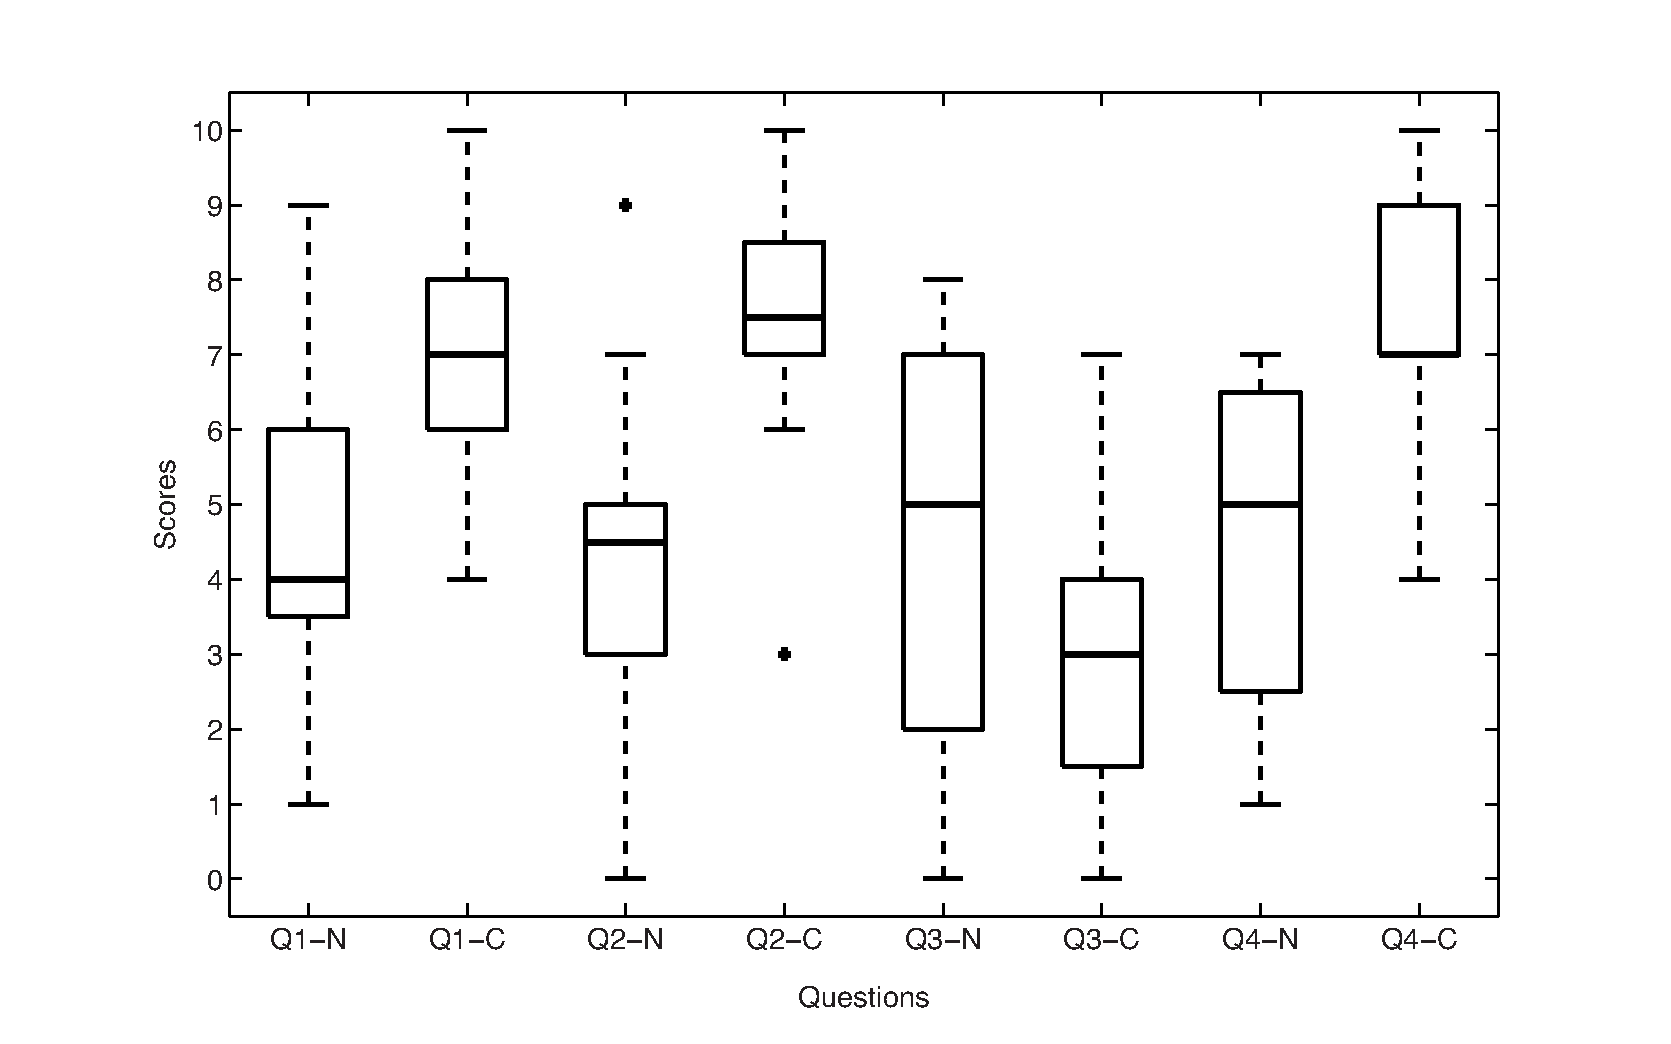
\includegraphics[scale=0.6]{figures/sens/Figure4.eps}
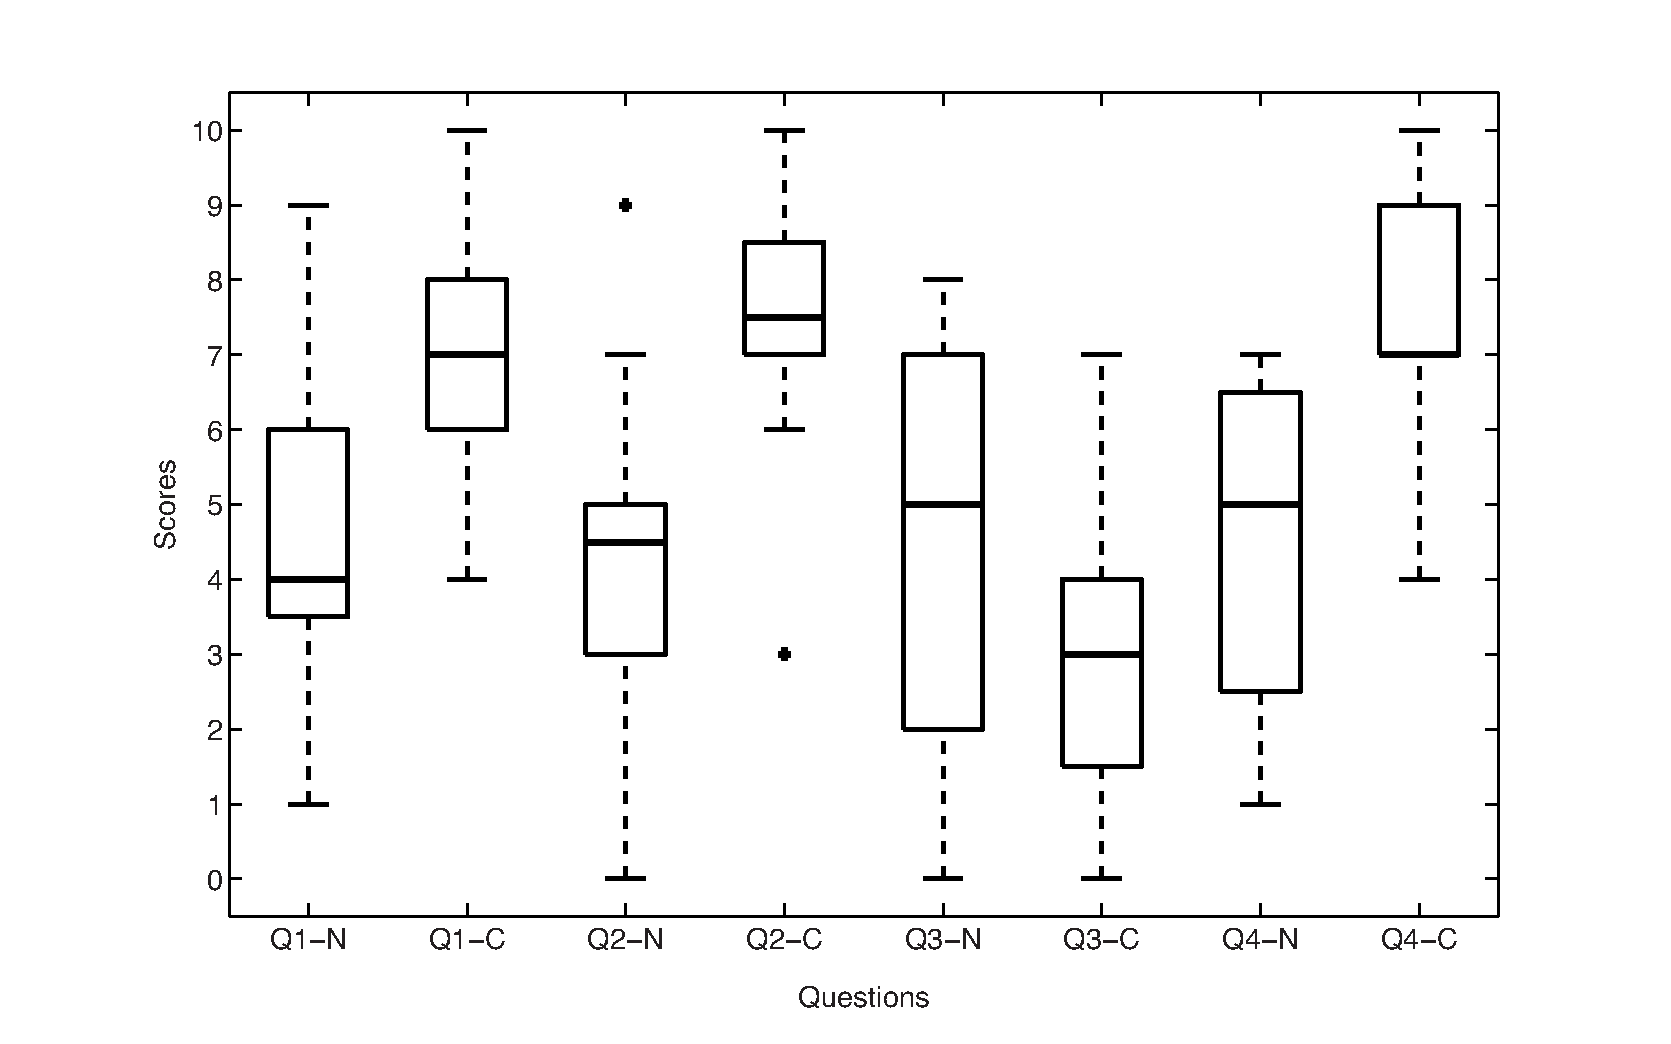
\includegraphics[width=10cm]{figures/sens/Figure4.eps}
\caption{Boxplots for the questionnaire scores for condition N and C. The central horizontal lines are the medians and the upper and lower edges of the boxes are the 25 and 75 percentiles. The whiskers extend to the minimum and maximum data points if these are not outliers. Outliers are shown separately and are outside the bounds of 1.5 times the interquartile range below or above the 25 and 75 percentiles respectively. In this case the length of the whisker extends to 1.5 times the interquartile range. }
\label{sens4}
\end{center}
\end{figure} 


Figure \ref{sens5}b shows the scatter diagram for the plot of \emph{log(tVR)} by \emph{log(tReal)} separately for the N and C groups. Analysis of covariance on Condition results in a common slope ($P < 0.00001$) with the intercept for the C group greater than that for the N group ($P = 0.020$). The residual errors are compatible with normality (Shapiro-Wilks, $P = 0.23$).



\subsection{Relationship between TST and the body ownership illusion}
 
The previous section shows that the change in TST is greater for the C group than for the N group. However, we also need to consider the relationship between the subjective illusion of body ownership and the TST. Figure \ref{sens6} shows scatter plots of  $\Delta log t$
 on each of the questionnaire responses Q1,…,Q4 together with the corresponding correlation coefficients and significance levels. The results show that there is a positive and significant correlation between  and Q4 (\emph{arm}), suggesting that the greater the level of perceived ownership of the virtual arm the more impaired is the sensitivity to temperature changes. Although the correlations with the other variables all point in the appropriate directions (positive for Q1 and Q2, while negative for Q3) only Q4 is significant. 

However, we have seen that the condition (N or C) is positively correlated with $\Delta log t$  and also with the questionnaire responses. So it could be that the correlation between Q4 and  $\Delta log t$  is spurious. This is unlikely to be the case though. The partial correlation coefficient between Q4 and  $\Delta log t$ , controlling for condition,  is  0.30  with a (two-sided) significance level of 0.065. On the other hand the partial correlation between condition and   $\Delta log t$, controlling for Q4, is 0.15 with a significance level of 0.356. Hence when controlling for condition the relationship between Q4 and  $\Delta log t$ is maintained. 

There is also another issue to consider. In \cite{Tsakiris2011} it was reported that susceptibility to the rubber hand illusion varies with interoceptive sensitivity (see discussion in section \ref{disc_embodiment}). It is possible that susceptibility to the body ownership illusion considered here may vary with exteroceptive (thermal) sensitivity. This does seem to be the case with respect to Q4. Figure \ref{sens7} shows the scatter plot of log(\emph{tReal}) on Q4 (\emph{arm}), which shows a significant negative slope. There are no significant correlations with the other questionnaire variables. This suggests that the greater the exteroceptive (thermal) sensitivity the greater the susceptibility to the illusion of owning the virtual arm. Now since we have found that log(\emph{tReal})  is correlated with Q4 and log(\emph{tReal})   is obviously correlated with  $\Delta log t$=log(\emph{tVR})  - log(\emph{tReal})  , the correlation between Q4 and $\Delta log t$  may be spurious for this reason. However, the partial correlation between Q4 and $\Delta log t$ controlling this time for log(\emph{tReal})  is 0.34 with $P = 0.034$, and thus the correlation is maintained.


\begin{figure}[]

\begin{center}

%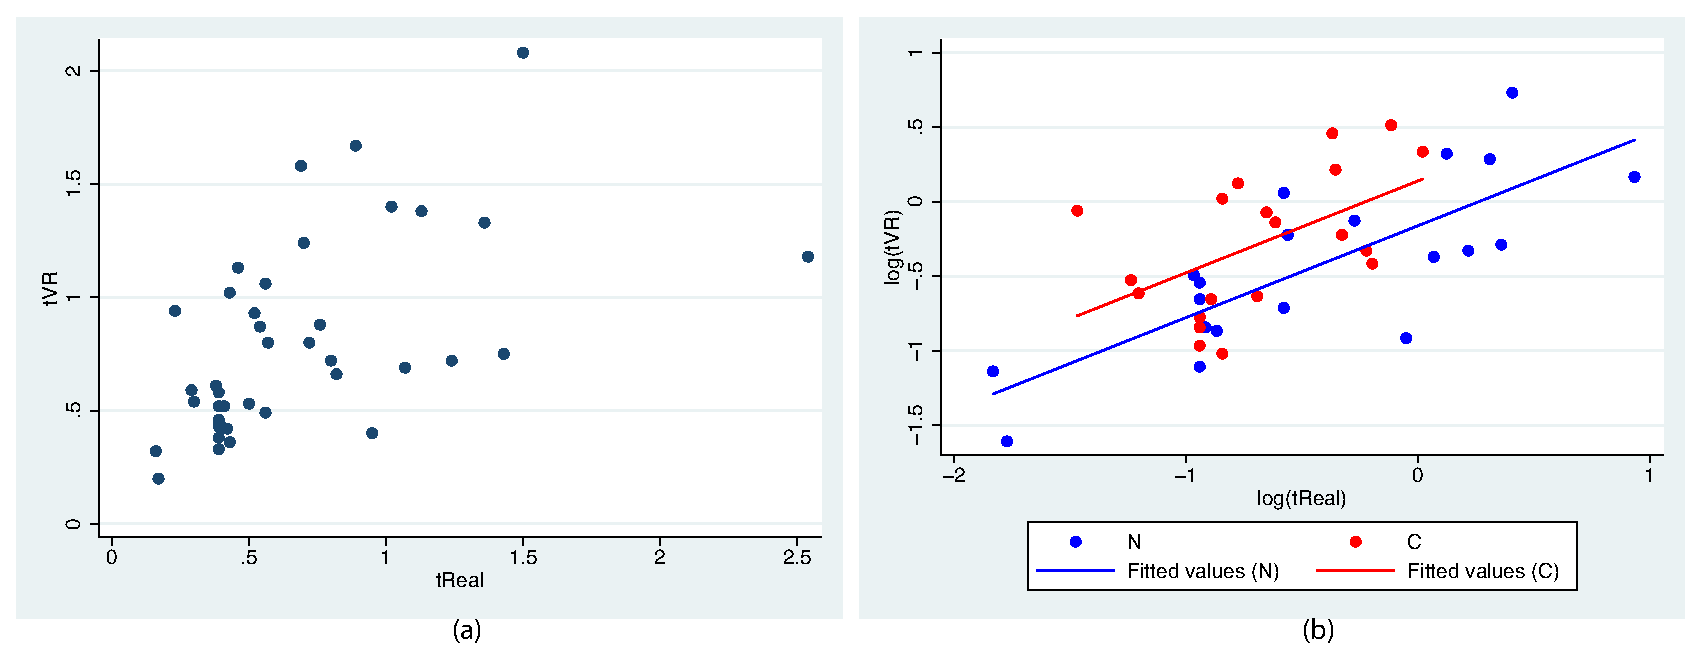
\includegraphics[scale=0.6]{figures/sens/Figure5.eps}
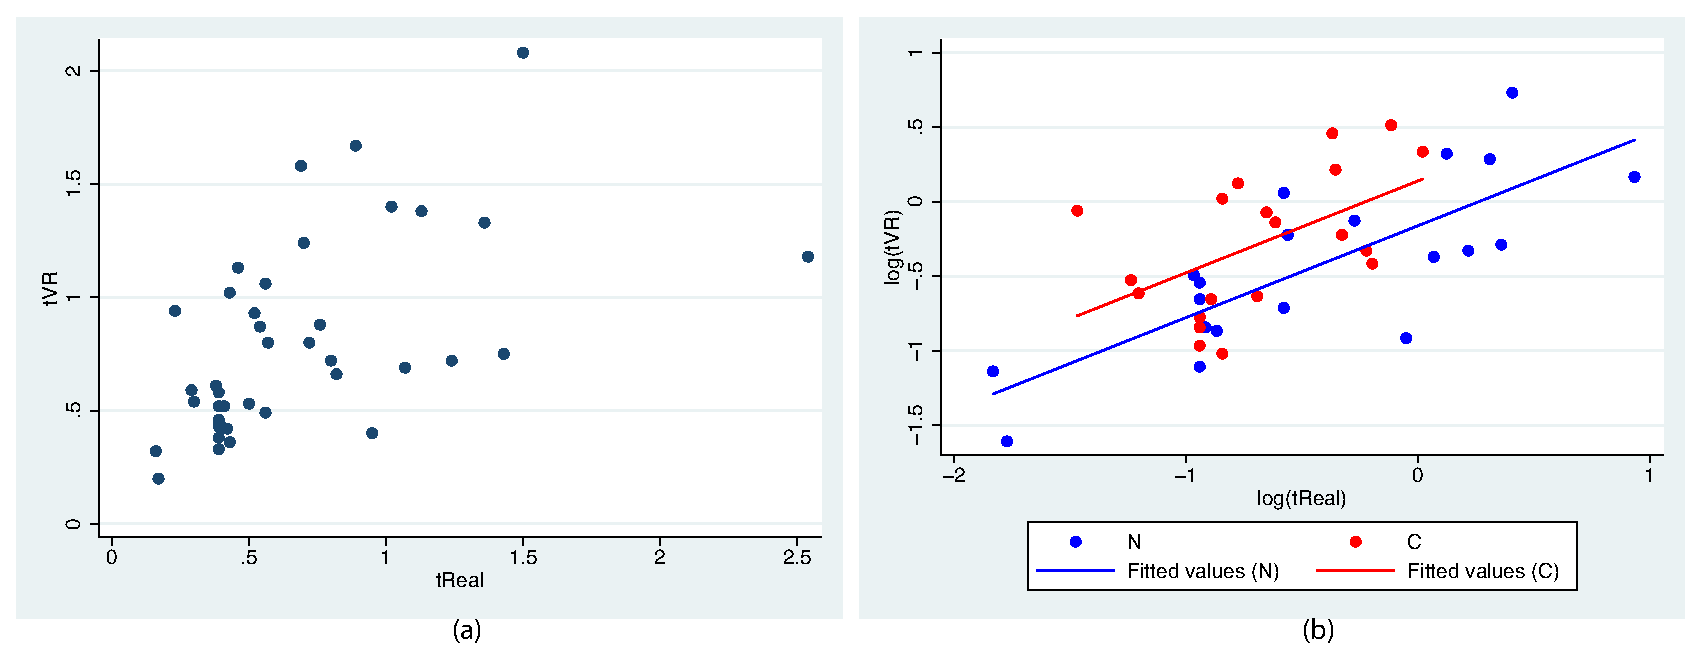
\includegraphics[width=12cm]{figures/sens/Figure5.eps}
\caption{Scatter plot of tVR by tReal (a) on the original scale (b) on the log scale, with regression lines for analysis of covariance with Condition as the co-variate. }
\label{sens5}

\end{center}

\end{figure} 


\begin{figure}[]

\begin{center}

%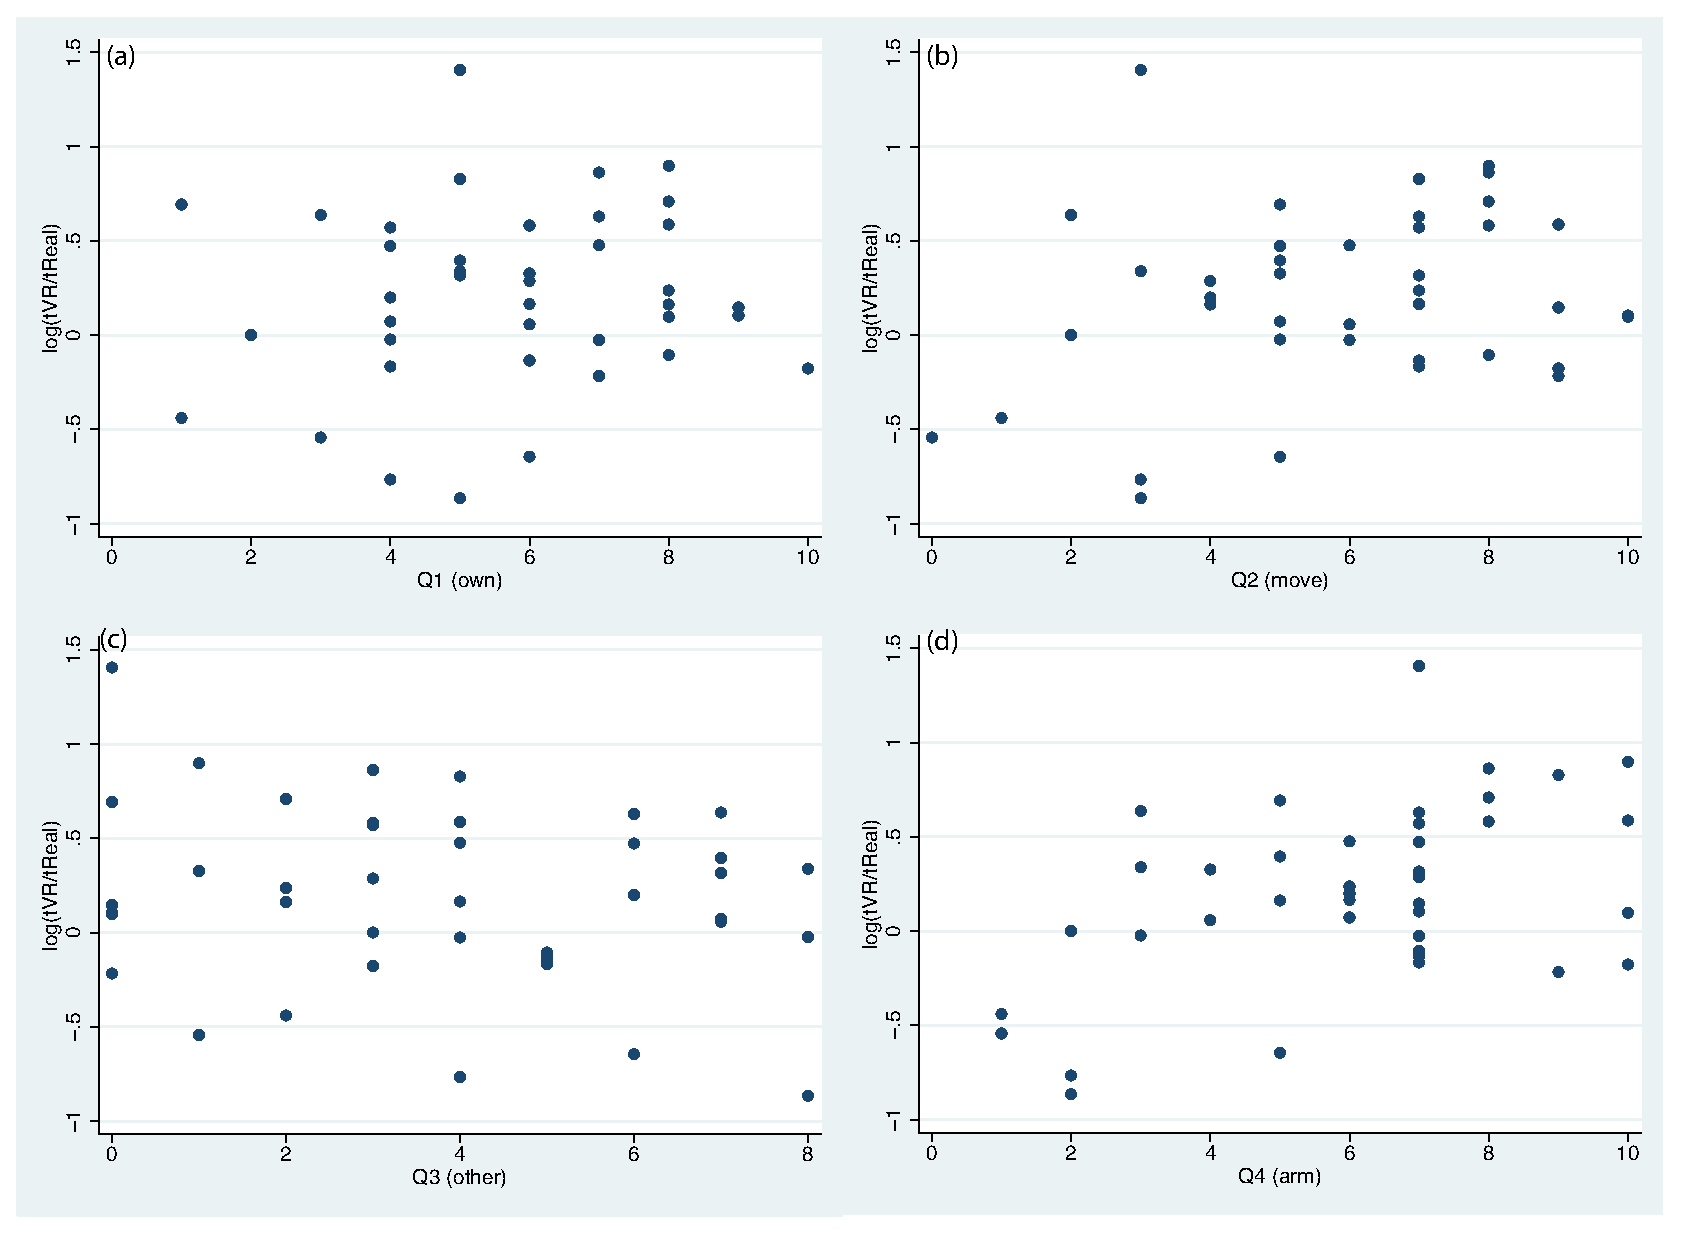
\includegraphics[scale=0.6]{figures/sens/Figure6.eps}
\includegraphics[width=12cm]{figures/sens/Figure6.eps}
\caption{
Scatter diagrams of log(tVR/tReal) by the questionnaire variables. 
(a) Q1 (\emph{own}), $r = 0.11$, $P = 0.49$. (b) Q2 (\emph{move}), $r = 0.24$, $P = 0.13$.   (c) Q3 (\emph{another}),        $r = -0.20$, $P = 0.22$. (d) Q4 (\emph{arm}), $r = 0.48$, $P < 0.002$. In each case r is the Pearson correlation coefficient, and P is the significance level against the null hypothesis of 0 correlation. All tests satisfy normality requirements on the residual errors of the corresponding regression equation using the Shapiro-Wilks test (all P for residual errors following a normal distribution $>$ 0.40).  }
\label{sens6}

\end{center}

\end{figure} 



\begin{figure}[]

\begin{center}

%\includegraphics[scale=0.8]{figures/sens/Figure7.eps}
\includegraphics[width=12cm]{figures/sens/Figure7.eps}
\caption{Scatter diagram of the scores for Q4 (\emph{arm}) on the log prior sensitivity measurement. $r = -0.40$, $P = 0.011$ (two-sided). Shapiro-Wilks test for normality of residual errors has $P = 0.36$. }
\label{sens7}

\end{center}

\end{figure} 


\section{Discussion}
\label{disc_embodiment}
This experiment has led to the following findings. First, the subjective illusion of body ownership (Q1), agency (Q2) and specifically virtual arm ownership (Q4) was significantly higher in the consistent condition than in the non-consistent condition (Figure \ref{sens4}), and the median scores in the consistent condition were high (around 7 out of 10). Hence it is possible to produce a quite strong subjective illusion of ownership of a collocated virtual body that is seen from a first person perspective position and in a virtual mirror, and where the body is in the same posture and the virtual right hand is slaved to the movements of the real right hand. When the body posture is not consistent with that of the real body and the movements of the virtual right hand are asynchronous and different than those of the real hand then the subjective illusion is significantly lower.

Various aspects of this result have been found before. In \cite{Sanchez-Vives2010} it was shown that a virtual arm and hand can be embodied through synchronous visual-motor correlation with the real hand, although since the display was on a stereo powerwall, the person could see their real body except for their hidden illuded hand. In \cite{Slater2010} a whole body ownership illusion in virtual reality was demonstrated that included the body seen from 1PP and a mirror reflection, but it also included synchronous visual-tactile stimulation. In \cite{Gonzalez-franco} a whole body ownership illusion was demonstrated where the virtual body was only seen in a virtual mirror and with upper body synchronous visual-motor correlation. The work in \cite{Petkova2008} incorporated a static manikin body seen from a 1PP but required synchronous visual-tactile stimulation. Finally \cite{Petkova2011} directly tackled the issue of 1PP versus 3PP and found that 1PP was essential for the generation of a body ownership illusion.

It is important to note that during the pilot studies it was difficult to find a condition in which there was a reduced ownership illusion when there was embodiment with a collocated body seen from 1PP. In the case study reported in \cite{Pena:Immersive:2010a} it was found that when someone is put virtually in a posture that is not their actual one but where that posture is feasible even if uncomfortable, then vision tends to dominate and the participant has the illusion of being in that posture. In the current experiment we found that by having an implausible (but physically realisable) body posture and the inconsistent virtual arm movements we were able to attain a wide range of ownership questionnaire scores. Even so note that the ranges of body illusion questionnaire scores for the Non-Consistent Condition were relatively high (Figure \ref{sens4}) notwithstanding that this body was not in the same posture and did not show same the mobile arm movements as that of the real body. However, the body trunk was collocated with the real body. In summary - a degree of subjective ownership over a collocated virtual body seen from 1PP seems to be the normal response, and not an exceptional one.

The second finding was that the experimental manipulation did result in significantly greater change in TST in the Congruent than in the Non-Congruent condition (Figure \ref{sens5}b). This supports the notion in \cite{Moseley2008a} that there may be dis-ownership associated with withdrawal of resources from the real body in the context of virtual body ownership. 
The third finding is that TST measured prior to entering virtual reality was negatively associated with the measured subjective illusion of ownership over the virtual arm (Figure \ref{sens7}).  In other words greater sensitivity to temperature changes prior to the virtual embodiment (lower TST) was associated with a greater subjective illusion of arm ownership. In \cite{Tsakiris2011} it was reported that susceptibility to the rubber hand illusion increases with lower interoceptive sensibility (specifically own heart beat detection). On the other hand in 
\cite{Mirams2011} it was found that when participants were asked to pay attention to interoceptive processes (heart beats) they were more likely to report the feeling of touch  in a somatic signal detection task, and less likely to report touch when they had been asked to increase exteroceptive attention.  In the current experiment participants had been asked to pay attention to exteroceptive signals prior to their virtual embodiment, and lower TST was associated with higher subjective illusion specifically of the hand of the arm used for the temperature sensitivity readings. Putting this together a conjecture would be that lower interoceptive sensitivity and higher exteroceptive sensitivity could be predictors of the likelihood of the virtual arm illusion. Of course, it is the case that we did not attempt to manipulate exteroceptive sensitivity as such, but only attention to this, but this conjecture is a reasonable claim from our own results together with these two papers. 
The fourth finding is that there appears to be a positive association between the illusion of virtual arm ownership (Q4) and the change in TST from prior to after the stimulation. In other words, lower temperature sensitivity in the VR correlates with higher ratings of virtual arm ownership. It should be recalled that it was only the arm that was moved during the experiment whereas participants had been instructed not to otherwise move their body except for the head. This result is analogous to that of \cite{Moseley2008a}
 where it was found that that the amount of cooling of the illuded hand was positively correlated with the strength of illusory ownership as assessed by questionnaire. It was argued that this demonstrated a significant drop in skin temperature for the real hand as a result of experiencing the rubber hand illusion. It was further noted that this also provided evidence of brain (illusion induced) changes in homeostatic control, and akin to what has been observed in patients as a result of ‘dis-ownership’ of limbs (for example, as a result of stroke).  In other words ownership of the rubber hand was accompanied by dis-ownership of the real hand.

 The results of the current experiment could be argued to lend supporting evidence to that conjecture, but in a different modality – sensitivity to temperature changes rather than actual temperature. 
In \cite{Folegatti2009} evidence was presented that the result found in \cite{Moseley2008a} of a decrease in temperature of the illuded arm may have been solely due to cross-modal incongruence rather than the subjective illusion of rubber hand ownership. The experiment reported in this paper tends to support the positions of \cite{Moseley2008a} rather than \cite{Folegatti2009}, since the partial correlations showed that even allowing for a direct effect of the experimental condition on the threshold change there is still an effect of the subjective illusion of arm ownership. A very similar result to \cite{Moseley2008a} was found, both the fact that the experimental conditions did result in a change in TST, and especially the seeming correlation between lesser sensitivity to temperature change associated being with higher levels of the arm ownership illusion. Moreover, once the cross-modal incongruence is itself accounted for (using the partial correlation) the apparent connection between the illusion level and sensitivity does not vanish.

There is general consensus that body and limb ownership are supported by a combination of bottom-up information (including visual, tactile, motor and proprioceptive) together with a top-down mechanism in the form of a cognitive representation in the brain dealing with decisions and actions and creating the sensation of control and agency over the body, which should be humanoid in form (for example \cite{Tsakiris_2010}).  In this model, the induction of virtual limb ownership would provoke a reduction in the detection thresholds because the sensory input coming from the virtual limb would not fit so well with the cognitive model of the body representation, and therefore this would suggest the tactile or temperature information to be less reliable. 

If we assume that the body representation has been built by integrating the sensory information over a long period of time, then this is consistent with general principles of brain organisation based on the minimization of the negative log-evidence or ‘surprise’ \cite[]{Friston2009}. We could say that because the limb looks strange or seems to be even slightly misplaced or moving slightly differently compared to the real limb, the brain does not completely ‘trust’ the information provided, and therefore reduces autonomic activity hence provoking a temperature drop \cite[]{Moseley2008a} and even greater immune activity \cite[]{Barnsley2011}.

This framework could be used to explain why in the current experiment some questionnaire responses are positively associated with sensitivity to temperature changes but not to virtual body ownership as a whole. Since in all conditions the trunk of the virtual body was collocated with that of the real body and it did not move, there was no visual-proprioceptive conflict with respect to the body trunk, which therefore does not provoke any conflict in the brain. Putting it another way, since the representation of the body trunk is collocated with the real body trunk, appears to look the same, and does not move - there is nothing to be ‘surprised’ about. However, the subjective feeling of ownership over a virtual limb that moves necessarily provokes a greater mismatch between the virtual representation and the real limb, which induces the brain to observe a mismatch between what the underlying body representation predicts as input and the sensory information it gets from the limb. This, in turn, would diminish the ‘trust’ and trigger the changes described. 

In other words, in the case of the body trunk that does not move, ownership is reinforced precisely because it is coincident with the real body and there is no sensory conflict. Hence this type of virtual body ownership does not imply real body dis-ownership, since this part of the virtual body is always static and coincident with the real one. Remember also that the participants even wore the same pullover as they could see in the virtual mirror being worn by their virtual reflection, or directly when they looked down towards themselves. However, the virtual arm is not in exactly the same place as the real one, does not look exactly like the real one,  and does not move exactly the same,  but it is nevertheless ‘close enough’ to be incorporated into the body representation. Therefore, there is probably at least a subliminal sensory conflict (in the C condition). The position of the hand is more sensitive than the body trunk, so small departures from reality have a large impact. However, in the N condition, the differences between real and virtual hand are so great, that the virtual hand is not even incorporated into the body representation.

On a larger scale, this explanation also seems to be compatible with increases in tactile discrimination provoked by displaying an augmented image of the real limb, but not of an augmented object \cite[]{Kennett2001}. Moreover, we could predict that an ownership illusion is maintained while progressively degrading the visual appearance of the limb, as in \cite[]{Hohwy2010},  ‘disownership’ of the real limb could be increased and a stronger reduction of temperature sensitivity or even of two-point tactile discrimination could be provoked, which may be useful in therapy for people suffering tactile hypersensitivity or similar disorders. Generally there has been increasing interest in the use of body ownership illusions in the treatment of pain.  For example, recently \cite{Hansel2011} and \cite{Longo2009} both show that pain perception is diminished in the context of the experimental setups to such illusions and our findings are in line with this. 

\cleardoublepage




\chapter{Trama: a cognitive story model}
\thispagestyle{empty}
%\markboth{\thechapter \ Trama: a cognitive story model}{}

\label{ch_trama}



\begin{origquote}
   Esa trama de tiempos que se aproximan, se bifurcan, se cortan o que secularmente se ignoran, abarca \emph{todas} las posibilidades.-- \cite{borges1942jss}\footnote{The usual translation in english translates \emph{trama} as \emph{network}: This network of times which approached one another, forked, broke off, or were unaware of one another for centuries, embraces all possibilities of time. However, the word \emph{network} doesn't capture the directional aspect of a story. Here, we would rather like to translate the previous as \emph{This} \textbf{Trama} \emph{ (...) covers all possibilities  }}

\end{origquote}



\section{Introduction}


In this chapter  we introduce a formal model of a story that can be used by a software agent.  The main motivation to introduce this model is to implement a method that transforms a set of events intuitively perceived as a story into an abstract representation that can be used as a  coordination plan when embedded within a set of situated agents. 
Using this model one can implement the principles of interaction introduced in chapter \ref{ch_zelig} within \emph{any} story, as long as they can be stated in a form similar to a movie script.


The basic intuition behind the formalism introduced is that to represent a story \emph{plot} we can use the formalism of lattice theory. This model is named \textbf{Trama}  because in catalan both \emph{plot} and \emph{lattice} are translated as \emph{trama}. 
To do so, we introduce a certain algebra which we name \textbf{Llogic}\footnote{ we name this algebra \emph{Llogic} -First sillab like Yogui, second like Logic- as a shorthand for \emph{Language Logic}, as they pretend to describe logic relations among language propositions. Also, in catalan this word is a dialectal variation of the word Logic.}. This formalism is used to relate the events forming a story within an abstract representation that can then be embedded within a set of situated agents performing real-time decisions in an immersive virtual environment.


The method is based on considering a story as a set of causally-related and goal-motivated events \cite[]{stein1982ds}. To model any particular story, we consider a story \textbf{S} to be a non-stationary process made of causally-related and goal-motivated events. To be able to satisfy this definition in a formal model, we introduce a novel definition of causal relation. Section 2 introduces the main mathematical definitions involved in the story model. Section 3 shows how such the events forming the story can be integrated within a set of situated agents. Section 4 shows how such model can be used to declare a plan in a way very similar to a movie script. 


\section{A logic for causally-related stochastic events}
\subsection{Introduction}

As said, we consider a story \textbf{S} to be a non-stationary process made of causally related and goal motivated events. Because it is not stationary, the probability $p$ that an event ‘$e$’ occurs changes across time. 

To characterize the problem it is important to notice that the probability of occurrence of an event may change for factors that are independent among them. For example, the probability of occurrence of an event `$e$' can increase or decrease if performing such event is expected to help achieving a particular goal, or prevent from achieving another one. The probability of occurrence of $e$ can also increase because of the occurrence of a preceding event. In this last case, one would consider the preceding event to be the cause of $e$.
 It is therefore important that different preceding events and separate goals can affect such probability of occurrence in a distributed fashion. %This suggests we should use a distributed decision mechanism, and that the way the story is integrated within the decision mechanism of a particular kind of situated agent should not affect its suitable properties (reactivity, adaptation, stability, etc).

In addition, given the principle of \textbf{Substitution} previously introduced, it should be possible that one agent replaces another one, despite each of the agents should be able to make decisions independently. Therefore, each of the different agents participating in the story should have an independent copy of the story. Finally, agents also need to be able to estimate in real time the likeliness that an event was performed by another agent or a human participant. To be able to address these different requirements, we define an event and a logic to relate the occurrence of different events as follows.


\subsection{Events}
\label{event_def}
\begin{table}[]
\caption{The data structure associated to each of the events forming a story has several elements.} 

%\centering
%\begin{tabular*}{0.90\textwidth}{@{\extracolsep{\fill}} |c | l| }
\begin{tabular*}{1.00\textwidth}{ p{0.15\textwidth}  p{0.80\textwidth} }
% centered columns (4 columns)
\\
\hline\hline
%inserts double horizontal lines

 & \textbf{An event forming a story is constituted of:} \\
 [1ex]
  \hline
% inserts table
%heading
%\hline
% inserts single horizontal line
name & A string containing the proposition associated with it \\
pos & A fuzzy value storing the possibility value \\
nec & A fuzzy value storing the necessity value \\
[1ex] 
\hline
context & It corresponds to $e^*$.  A logical condition over an array of pointers to the events forming its context\\
cause & It corresponds to $e^{**}$. A logical condition over an array of pointers to the events that could be the cause \\ 
pEstimator & (A pointer to) an estimation method to check whether some other agent actually performed the action\\
isInternal & A boolean value to store if the event is external or internal\\
[1ex] 
\hline
TTime & The triggering time, this is, the moment when the event is triggered, (or considered to be so by the agent doing the estimation) \\
pSpreading & (A pointer to) a method determining whether enough time passed after the cause occurred. This will be used to decide whether the event can occur\\
[1ex] 
\hline
%inserts single line
\end{tabular*}

\label{table_event_ch:trama}
% is used to refer this table in the text
\end{table}



Each event is associated with a label, which can be $a$’,`$b$’, `$c$’, etc, or a proposition such as ‘\textbf{Mike starts running}’. In addition, all events have a context. For an event ‘$e$’, the context ‘$e^*$’ is a condition over preceding events that makes the event can occur. This does not mean it must occur, but only that it is possible it occurs. For example, in order to smoke a cigarette one needs, besides a cigarrette, to have a lighter. However, having the lighter nearby is not the cause of smoking a cigarette. It only makes it possible. 

We also need to distinguish between \emph{external} and \emph{internal} events. An internal event $i$ is an event whose cause $i^{**}$ is a previous event in the story. If there are several possible causes, they are all previous events in the story. External events do not have a cause as part of the events forming the story. In order to manage the causal relations between internal events, we consider all internal events have a triggering moment and a duration. For each pair cause-consequence, these intervals will be used by a time-depending function to determine the speed at which the effect of a cause spreads to its consequence.

In addition, because each situated agent will have to coordinate with the agents doing different actions forming part of the story, an internal event `$i$’ can also have an estimator ‘$\hat{i}$’ associated. Contrary to an internal event, an external event ‘$e$’ can only be estimated, and therefore it must have an estimator ‘$\hat{e}$’ associated. 
Finally, to relate the occurrence of events we consider each event has 2 fuzzy values associated, a possibility and a necessity. One can therefore define an event with the  table \ref{table_event_ch:trama}.


\subsection{Llogic operators}
\label{llogic_oper}
To relate the occurrence of the different events forming the story some kind of logic is needed. And here, we face a dilemma. Lattice theory defines logics over partially ordered sets and seems ideal to control how the causation spreads among different events. However, considering  events as discrete things that are partially ordered would imply their occurrence is deterministic. 

In this application scenario different agents –some of them human partici-pants-- will perform different parts of the story. Therefore, some of the events will have to be estimated, and the likeliness of an event having occurred should affect the likeliness of occurrence of its consequence. This suggests that Possibility Theory \cite[]{zadeh1999fuzzy} could be a good candidate. However, there is no natural way to define an implication operator in Possibility Theory, where the temporal order of events is not generally considered. %In addition, it would be desirable to embody our plan within a set of situated agents minimizing at most the impact on suitable properties it has –reactivity, stability, distributed decision mechanism, etc-.

To address these needs we define a logic that combines these 3 elements. In order to conceal the different properties they have, we consider a story to be defined in 3 steps: a declaration, a quantification and an instantiation.  Each step determines one aspect of the relation between events: the declaration determines the partially ordered temporal relations between the events. This means that when we state the events forming a story we are implicitly saying which events start before or at the same time than others. The quantification step determines how the  likeliness of occurrence of an estimated event spreads to subsequent events. The instantiation determines the temporal dynamics of how this spreading occurs.  %the chains of causal relations spread within a particular set of situated agents. 
The \textbf{Llogic} operators that are used throughout these 3 steps %allow going from a logical description to a quantified description
 are defined as follows:


   \begin{itemize}
        \item  \textbf{AND}($\wedge$) is defined on the \emph{necessity} domain:
\begin{equation*}
 nec(a \wedge b)\triangleq min(nec(a),nec(b))
\end{equation*}
        \item \textbf{OR} ($\vee$) is defined on the \emph{possibility} domain:
\begin{equation*}
pos(a \vee b)\triangleq max(pos(a),pos(b))
\end{equation*}
          \item \textbf{IF x THEN y } ($\Rightarrow $) : Implication transfers values from the possibility domain to the necessity domain, and it assumes that the given consequence is possible. Therefore, assuming $[pos(y)=1]$, the implication is defined such as 
\begin{equation*} 
x \Rightarrow y \triangleq  nec(y):= pos(x) \end{equation*}
   \end{itemize}

In the previous definition the sign `$:=$' means `assign value on the right to variable on the left', like in any standard programming language. The time at which this assignment will occur will depend on the dynamics of the spreading of possibility and necessity values through the chains of causal relations %which are only fixed at the third step of our logic, 
when the story is embedded within the situated agents. 


It should be noticed that these logical operations are not commutative. Intuitively, the 2 propositions ‘\textbf{He gets angry AND she cries}’ do not imply the same as ‘\textbf{She cries AND he gets angry}’. The causal relations suggested by these sentences are not the same, and they do not suggest the same meaning. Therefore, quantifying the likeliness of one of these sequences occurred does not say anything about the occurrence of the other. Intuitively, the meaning of a formula like ‘$a\wedge b$’  is better captured if instead of reading as ‘a and b’ one reads it as ‘a and then b’.  The same goes for $\vee$. On the other side, these `$\wedge$' and `$\vee$' operators do satisfy the usual associative and distributive properties. For example, ‘$(a \wedge b) \wedge c$’ is equivalent to ‘$a \wedge (b \wedge c)$’,  and ‘$(a \vee b) \Rightarrow c$’ is equivalent to ‘$(a \Rightarrow c) \vee (b \Rightarrow c)$’.

Other operations can also be defined. For example, it is useful to consider a \textbf{NOT} operator such as:
\begin{itemize}      
        \item  \textbf{NOTP} ($ \neg$) The negation operator has the particularity of being multi-valued. 
\begin{equation*}
 pos(\neg ( a,b,c )) \triangleq 1 - max(pos(a),pos(b),pos(c)) 
\end{equation*}
   \end{itemize}

The reader might have noticed that the definitions of \textbf{AND} and \textbf{OR} are equivalent to usual possibility theory \cite[]{zadeh1999fuzzy} . However, the definition of negation is not. In possibility theory, the transfer between the possibility and necessity domains is done considering the negation over the complementary set: Given $COMP(a)$ is the complement of $a$, $nec(a)=1-pos(COMP(a))$.  Here complementary sets are not considered, but rather partially ordered sets of events. %This is why to connect the possibility and necessity domains we introduce an alternative mechanism: causes and contexts to spread the possibilities and the necessities. 



\subsection{Causes and contexts}
\label{caus_and_cont}
With the previous logic we can define the context and the cause of an event and how they determine its possibility and necessity values. For each internal event ‘i’:
\begin{itemize}
\item
	The context $i^*$ is a chain of preceding events such as $i_1\wedge i_2\wedge… \wedge i_n$. where $i_1 … i_n$ are internal events that occur not later than $i$. This can be stated simply by saying the triggering times satisfy this relation: $t_{i^*} \leq t_i $.
The context fixes the possibility value, with the formula: $pos(i) = nec(i^*)$. In addition, it is convenient to consider that all elements of the context must be internal.

\item	The cause $i^{**}$ is a chain of preceding events such as $i_{n+1} \vee i_{n+2} \vee … \vee i_m$. The cause fixes the necessity with the formula: $nec(i):= pos(i^{**})$. Note that because ‘$\vee$’ is quantified with a ‘$max$’ operation, in the spreading mechanism only 1 of the elements listed will be the \emph{actual} cause. The actual cause can be an internal or an external event.
\end{itemize}


The reason why we define a cause and a context in such a way is that we can associate a lattice to each internal event ‘$i$’ where ‘$i$’ is the top element and the \emph{actual} cause in ‘$i^{**}$’ is the pseudo-complement of the context ‘$i^*$’. In this construct, it can be shown that the implication operator ‘$\Rightarrow$’ corresponds to the definition of implication in a Heyting algebra \cite[]{rutherford1965ilt}. This is the central mathematical insight of the logic here introduced: a generalization of possibility theory replacing the idea of set complementation with the notion of lattice \emph{pseudo-complement}.
 Thus we obtain sequences of partially ordered events whose occurrence is related through fuzzy rules.

It should be stressed that the definitions of cause and context do not apply to external events. The reason is simple: by definition an external event does not have a known cause. This is why it has to be estimated. External events do not have a necessity value, and the estimated likeliness of occurrence will be considered as its possibility value. This is also the reason why within a plan we consider negations ($ \neg$) or disjunctions ($\vee$) of external events. On the other side, internal events do not relate through disjunctions and negations because by definition they must all occur. 


As we will show in detail in section 4, these operators can be used to process a story declared as a movie script and embody it in a set of situated agents. However, we first need to choose what kind of situated agent will be used and define how a story event is integrated within its decisional procedure.



\section{Causally-related events within situated agents}
\subsection{Election of the architecture}
As said before (see section \ref{soa_sa}), \cite{Maes1989} introduced goals in situated agents to give them a direction or purpose rather than purely reactive behaviors. In this view, an activation spreading mechanism would select which \emph{actions} were most relevant to achieve a certain number of \emph{goals} according to particular \emph{perceptions} of the state of the world was introduced. This allowed agents to use knowledge based on simple empirically testable rules with techniques of statistical learning \cite[]{maes1991ana}.

Taking on these results, \cite{dorer1999bnc} introduced a particular kind of behavior network that made decisions over continuous and dynamic environments. He showed it could be used for a robot playing football with real time decision-making, as exemplified in the Robocup competition. He also showed these networks behaved better than Maes’s decision mechanism (see also \cite{nebel2004behaviour}). \cite{dorer2004ebn} extended these results by introducing the use of \emph{resources} needed to perform an action. With \emph{resources}, the activation spreading becomes a concurrent mechanism that can select several actions simultaneously and always converge towards a decision. Extended Behavior Networks (\textbf{EBN}) were born. 


In summary, an \textbf{EBN} is a distributed decisional process defined by the declaration of Goals, Competence Modules and Resources. 
Competence Modules encapsulate knowledge in the form of preconditions and expected effects, and they spread perceptions and trigger actions.  Resources can be perceived and be used to perform actions associated with effects. 
 Each Goal and Competence Module can be declared separately. Therefore, it allows for the integration of a large set of skills and goals and it is easy to scale. Moreover, the modules are labeled, and therefore the function of each module in the whole is still understandable. It has suitable mathematical properties such as scalability, stability and convergence.
 
Since their introduction, \cite{DaSilvaCorreaPinto2005} have used this architecture to characterize personality stereotypes that would affect decisions of virtual characters in videogames. It has also been shown useful to model psychological aspects of decision-making. \cite{johansson2009affective} extended the architecture to show how it could integrate emotional traits in decision-making. \cite{dorer2010modeling} showed the decision mechanism could be adjusted to fit with realistic psychological biases in the context of risk estimation. This suggests virtual characters equipped with an \textbf{EBN} could show a certain psychological realism when interacting with a human participant.

On the other side this election is not the only one possible. \cite{goetz1998arb}  already showed that such action selection mechanisms could be seen as a particular kind of recurrent behavior network. A behavior network is a distributed decision mechanism over non-linear time varying domains. It has properties similar to a recurrent neural network, with the practical advantage that knowledge is encapsulated in labeled modules whose function can be interpreted. In this view, we may consider an action is considered as an attractor within a space of motivations. The strength of the attractor is defined by the expected effects of the action in relation to the fulfillment of the predefined goals. When the perceptions about the state of the world are updated, it changes the strength of the different attractors. If we are nearby an attractor, the mechanism of activation spreading will ensure we converge towards it. 
This means that the different goals will define an abstract space of motivations in which one or another action will behave as an attractor, and it will be selected according to whether they are expected to satisfy one or other goal. %The fact that it converges grants the decisional algorithm will not get stuck. This means a decision will always be updated according to the real time detected situation. The use of an activation spreading mechanism grants each the modules can be updated independently of the others, and thus the resulting architecture is distributed and can run concurrently.  In general, this will result in a situated agent that, from a physical perspective, is better characterized as a non-linear and time-varying system. It will take as inputs several perceptions on a continuous or discrete domain, and result in several actions selected, eventually with particular intensities.
 
%This suggests method developed in the following section for \textbf{EBN} agents could be adapted to other kind of decisional architectures showing the same mathematical properties. The only thing that would be needed is to change how the relations established with the \textbf{Llogic} operators are instantiated in this kind of decisional procedure.

\subsection{How to instantiate the events forming a story in a set of \textbf{EBN} agents}
\label{instantiate_events}
Once the kind of situated agent preferred is chosen, one needs to define how the events forming the story can be instantiated in a set of \textbf{EBN} agents without changing its properties. Here we provide an overview of how it is done. The reader interested in further implementation details should read appendix \ref{tramabot}.

The two central elements of an \textbf{EBN} are \emph{Goals} and \emph{Competence Modules}.
\emph{Competence Modules} have \emph{preconditions}, \emph{resources} and \emph{expected effects}. Taking a closer look at the decision procedure of the \textbf{EBN}, \emph{each} module considers the satisfaction of the preconditions as a fuzzy value determining its executability. This value is weighted with an activation level resulting from comparing the expected effects of the module with the different goals of the agent and preconditions of other modules. If this weighted product exceeds a certain threshold, then the algorithm will check, for \emph{each} resource $res$ used by the module, whether the amount expected to be used $T_u$ is bigger than the amount available $T_r$. These values are checked at decision time. This means that, given a state of the world $s$, what is checked is whether: $[T_u(res,s) \leq Tr(res,s)]$. 

\begin{figure}[]

\begin{center}
\includegraphics[scale=0.3]{figures/EBN1.jpg}
%\includegraphics[width=12cm]{figures/EBN1.jpg}
\caption{A schematic view of an agent in Extended Behaviour Networks. It has several goals and can use resources to perform actions if they are within the domain of his competence modules.}
\label{fig_EBN1}
\end{center}

\end{figure}

\begin{figure}[]
\begin{center}
\includegraphics[scale=0.3]{figures/EBN2.jpg}
%\includegraphics[width=12cm]{figures/EBN2.jpg}
\caption{In Extended Behaviour Networks an action will be performed if its effects are expected to meet the goals of the agent and the needed resources are available}
\label{fig_EBN2}

\end{center}

\end{figure}

\begin{figure}[]

\begin{center}
\includegraphics[scale=0.3]{figures/EBN3.jpg}
%\includegraphics[width=12cm]{figures/EBN3.jpg}
\caption{The essential modification introduced to manage stories is that action performing generates resources available for other agents, and that these resources are needed to perform the behaviours involved in a narrative plot.}
\label{fig_EBN3}
\end{center}
\end{figure}



To process the possibility and necessity values relating the events forming the story, we consider, for each event, its possibility to be a precondition, and its necessity a resource available ($T_r$). This implies that in order the event or action $a$ is executed the elements of its context must have already occured (or at least have started) and, in addition, the “amount of the resource ‘cause’ needed” is smaller than “the amount of resource ‘cause’ available”. This also implies that the temporal dynamics of %in which the possibility and necessity values spread through the activation spreading mechanisms of the EBN will be controlled by the $T_u$ values of the different competence modules triggering the different actions involved in the plot.  In other terms, 
how the necessity values spread through the chains of causal relations can be controlled in each module adjusting the $T_u(a,s)$. 



If one goes back to the definition of an event, the only element that is not completely defined  is what does the pointer pSpreading point to. In this case, it seems quite natural to point it to $T_u$. But then, which is the method that fixes the value of $T_u$? In the present application scenario, we consider the person defining the Story will provide a time interval in which each of the events should occur in order the story to unfold appropriately. This interval will be determined relative to the occurrence of some of the preceding events. For example, given an event $e$, the author of the story would determine it must be triggered between 3 and 10 seconds after its cause $e^*$ occurred.


We therefore assume the story creator will provide, for each event or action $a$, a temporal interval $[T_{min}, T_{max}]$ in which each it should occur. To grant the event occurs  within $[T_{min}, T_{max}]$, it is enough to use a function such as: 
\begin{equation*}
T_u(a,s)=1-\frac{(t-T_{min})}{(T_{max}-T_{min})}
\end{equation*}
 where $t$ is the current time in that interval. However, in principle it could be any other function. For example, if in a different application scenario one wanted to trigger an event after a chemical reaction finished, one could exploit information on pressure and temperature to estimate if the reaction finished and adjust the $T_u$ accordingly. 
In conclusion, to process all the events that are part of a story within a set of \textbf{EBN} situated agents, it is useful to consider each event to be an action but also a resource (see also figures \ref{fig_EBN1}, \ref{fig_EBN2} and \ref{fig_EBN3}).



In addition, to grant there will be a motivation to perform all the events we also define, given a story or plan ‘\textbf{S1}’,  an abstract goal which incites each agent to ‘Advance The Plot S1’ (\textbf{ATP\_S1)} whenever he can. This, together with the \textbf{Llogic} relations, implements the \textbf{Providence} principle introduced in the previous chapter.

When one instantiates a story \textbf{S} in a set of \textbf{EBN} agents, one might want particular actions to be assumed by particular agents or kind of agents. For example, in a story one might want to impose a certain role may only be assumed by an adult female character, but not by a male or a child. To impose those restrictions, it is enough to declare roles such as \textbf{MIKE}, \textbf{JOHN} as specific resources associated to the different events $a.b.c…$ As any other resource, each time an agent picks a role, it is blocked and no other agent can use it anymore. In the same way in videogames different characters have different skills, here we can simply limit, for each agent, which role resources he can adopt. This ensures the control over the \textbf{Substitution} principle introduced in the previous chapter.


\subsection{Why does such embodiment work?}
 
Why such way of embodying a story within a set if situated agents satisfies the definition of a story given before? Is a story implemented with such a method really a non-stationary process made of goal-motivated and causally related events? Given the decision mechanism of an \textbf{EBN}, the probability that a given module triggers a behavior will change according to three factors: 
\begin{itemize}
\item The extent at which the preconditions of the module are satisfied
\item 	The extent at which expected effects of performing the action are relevant for the goals of the agent
\item 	The extent at which the resources needed to perform the action are available
\end{itemize}
For the case of an event ‘$a$’ forming part of a story, the fact that its context is part of the preconditions ensures that, while the context is not satisfied, at least at certain extent, the possibility value associated with the event is zero. The event cannot occur, and its probability of occurrence is zero. 

Once the preconditions associated with performing the action $a$ are satisfied the probability of occurrence depends on the relation between the different goals of the agent and the expected effect associated to performing the action. For the events part of the story, there will always be some motivation to perform the action $a$ because of the fact that there is an ‘\textbf{Advance The Plot}’ goal associated with these. However, the probability this action $a$ is selected can depend on other goals of the agent, and the relevance of these goals will generally depend on the real-time perception of its environment and internal sate. It is therefore not possible to estimate the probability of occurrence of an event $a$ at a given moment without taking into account factors that are independent from the story. In particular, one must consider the different goals constituting the motivation to perform action $a$, the real-time evaluation of the environment and  of the internal state.

Despite the fact that this probability is not fixed by the definition of the story, it is possible to control how it evolves in time. In particular given a resource ‘cause’ available and needed for an action $a$ (these are $pos(a^{**})$ and $T_u$), the selection mechanism grants that the probability an action is selected will increase as the resources available become greater than the ones needed. 
Assuming there will always be at least 1 agent who can assume the particular role associated with the action, the way the cause is embodied grants that the event will occur within the predefined temporal interval. This is easy to see in the extreme case: once $t=T_{max}$, the expected amount of ‘cause’ resource needed is zero. Therefore, for any $nec(a)$ bigger than 0 the amount of resources needed will be smaller than the amount or resources available. If the action has not been performed yet the selection mechanism will select it on the basis that the action is expected to contribute to the \textbf{ATP} goal (and eventually to others). It is therefore certain that the action will be selected, and its probability of occurrence is 1. Finally, once the event has occurred the possibility value is set to 0 and the necessity value is kept unchanged. At this point one should consider the probability of occurrence is not defined because it is an impossible event: the event cannot occur.

The 2 fuzzy values, its possibility and necessity ($pos(x), nec(x)$) are stochastic variables associated to each event, but they change through time according to preceding events. These items are the basic mechanism to control how causes provoke consequences over time intervals.  Intuitively,  the possibility value reflects the extent at which a certain event is possible, meaning by this that it can occur. On the contrary, a necessity value determines the extent at which an event must occur. These values also apply to past events: an event might have possibly occurred, or must have necessarily occured.

Overall, this formalism has a certain parallelism between the possibility and necessity values as defined in possibility theory. In both cases, given an event ‘$a$’ its probability of occurrence $p(a)$ is bounded by these 2 values ($nec(a) \leq p(a) \leq pos(a)$). However, in our case this relation only holds when the event is about to occur, or it has actually occurred, something that can be seen as a ‘present region’ of the event, when the possibility is not zero. 
Correspondingly, one can define the ‘future region’ of the event when the possibility and the necessity of the event are zero, and the ‘past region’ when the possibility is zero and the necessity is not. In this last case, the event cannot occur again but, because its necessity is not zero, it can affect causal chains and provoke the occurrence of subsequent events (see also figure \ref{fig_basic_pos_nec}). The probability of the event is not defined because its occurrence is impossible. One can speak of the event as a \emph{fact} with a certainty of $nec(a)$.

\begin{figure}[tb]
\begin{center}
%\includegraphics[scale=0.5]{figures/basic_pos_nec.png}
\includegraphics[scale=0.5]{figures/basic_pos_nec2.png}
%\includegraphics[width=12cm]{figures/basic_pos_nec.png}
\caption{For \emph{each} event, its occurrence in time is bounded by two values, a possibility and a necessity. These values also allow the definition of the past, present and future of that event. }
\label{fig_basic_pos_nec}
\end{center}
\end{figure}

In other terms, a future event has a zero possibility and a zero necessity. As its context is satisfied, or it is estimated to have occurred, its possibility is updated to a value between 0 and 1 and it becomes a present event. As the cause of an event spreads, its necessity of occurrence increases. This increases the probability of occurrence, which can also be affected by other independent goals and causes. Finally, once a situated agent has performed the event, its possibility is set to zero, making it a past event that cannot occur but can affect subsequent events. Assuming the different agents inform each other on what they perform, or that the other agents can detect such occurrence autonomously, they will all coordinate their real-time decisions in order to satisfy the different constraints of the story.



Note in this formalism the probability of occurrence is never defined, only bounded. This is because the probability of occurrence of an event can change for reasons that are independent to the story. For example, given an interactive scenario a virtual character with specific goals or a human participant very motivated in some particular direction might decide to perform an action as soon as it is possible. On the other side, a very lazy character will only perform an action when it is strictly necessary. Therefore, the actual probability of occurrence of an action at a particular moment can depend on additional factors independent from the story itself.




\section{A story for situated agents}

\subsection{Introduction}
To process a story \textbf{S} using the formalism introduced in the previous section, we proceed in 3 steps.
\begin{itemize}
\item	The first step states the temporal order of the events forming the story in a way that looks very similar to a movie script.
\item	The second step is an automated mechanism that parses the movie script and quantifies the different events in terms of possibility and necessity relations. 
\item	The third step automatically integrates these relations within a set of decisional agents.

\end{itemize}

Each step uses one of the 3 levels of the logic previously introduced. We name such picture of a story the \textbf{Trama} story model. For example, lets consider a story occurring within a larger Star Wars scenario. The plot could involve the following events, stated with the typical conventions of movie scripts: 


\begin{quote}\begin{small}\bf
MIKE and JOHN are exploring the surface of a planet. ASSAULT SPACESHIPS arrive and start bombing. MIKE and JOHN ask for instructions to MOTHER SHIP, who replies that they should go to a bridge and cross it, where they will be picked up. MIKE and JOHN go towards the bridge. MIKE and JOHN arrive to the bridge and realize it is broken. The MOTHER SHIP orders to jump. MIKE jumps. MIKE reaches the other side. JOHN also jumps, but falls. The MOTHER SHIP asks what happened, but no one replies. The MOTHER SHIP saves MIKE.\end{small}
\end{quote}

This \emph{plot} can be considered as a set of propositions $a.b.c…$ that a group of situated agents should perform. In this view, different agents will integrate within their \emph{goals} the \emph{plot}, adopt a \emph{role} in it and contribute to it whenever relevant. Before entering in the details of how such a script can be processed by situated agents, we need to consider human participants can adopt one of the roles of the story, for example \textbf{MIKE} or \textbf{JOHN}.

\subsection{How to integrate the participant's behaviour in the story}

Now, consider how a participant into this story, if rendered in the context of an immersive virtual environment (IVE) where the story is being played out. How can we integrate the participants’ contribution? For example, to render the previous example in an IVE, if the participant adopts the role of \textbf{MIKE}, another agent will have to adopt the role of \textbf{JOHN}. However, if he does not, then we need to grant a virtual character can adopt his role.

In addition, it is also possible the participant assumes the \emph{role}  of \textbf{JOHN} but does not jump. In this case, the scriptwriter might consider another virtual character should replace him, adopt his \emph{role}  and jump. However,  the scriptwriter might consider an alternative way to go through the story and obtain the same outcome. This can be stated considering events that could occur in the story, but whose occurrence is not mandatory. For example:


\begin{quote}\begin{small}\label{the_script}
{\bf
S:

MIKE and JOHN are exploring the surface of a planet. ASSAULT SPACESHIPS arrive and start bombing. MIKE and JOHN ask for instructions to MOTHER SHIP, who replies that they should go to a bridge and cross it, where they will be picked up. MIKE and JOHN go towards the bridge. MIKE and JOHN arrive to the bridge and realize it is broken. The MOTHER SHIP orders to jump. MIKE jumps. MIKE reaches the other side. 

 \ \ \	IF JOHN jumps THEN JOHN falls. 

\ \ \	OTHERWISE bomb reaches JOHN.

JOHN dies and the MOTHER SHIP asks what happened. The MOTHER SHIP saves MIKE.
}
\end{small}
\end{quote}


In general, in an interactive story there can be elements that will be triggered or not depending on the behaviour of the participant. In the previous example, the character assuming the role of \textbf{JOHN} will fall only if he decides to jump. 
The \textbf{OTHERWISE} declaration simply states what should occur if John does not jump. These alternatives are the natural consequence of adopting the \textbf{Substitution} rule. As discussed in the previous chapter, virtual characters will not assume a pre-established role, but rather have to assume one role or another according to what the participant does. Apart from this, the story will unfold as a classic story.

Using the same syntax, however, the scriptwriter could introduce forking paths. For this it would be enough to state additional events after \textbf{JOHN falls}. Note that using this syntax the story writer can consider forking paths but, contrary to other approaches to interactive stories, such alternatives are not necessary. In the general case, the story is processed as a collaborative game in which each of the agents simply incorporates the \textbf{Substitution} rule: if the behavior of the participant (or another agent) suggests he is adopting a particular role in the story, each of the agents will assume that agent assumed that role and treat him consistently. Otherwise, if no one has adopted a particular role, and the role is available to a particular agent, then the particular agent will assume it and help to unfold the story. 


\subsection{A story declared in 3 steps}

To define a story using the logic previously introduced one only has to state the events that must occur, and in what temporal intervals. Obviously, as for any story rendered in an audiovisual environment one will also need to generate the animations corresponding to each event, but here we focus in the decision-making part.

\subsubsection{Step 1: Declaration}
\label{logic_des}

The first step simply consists in stating the events forming the story. We call this declaring the story. For example, it can be the events stated in  section \ref{the_script} involving \textbf{MIKE} and \textbf{JOHN}. Despite at this stage the story looks similar to a movie script stated in natural language, there are particular syntactical conventions respected. Each sentence is followed by a point ‘.’. The roles actively involved in an event are  stated with capitals. These conventions are typical from movie scripts, but one can also use them to define which are the events forming the story, which are the partial order relations between them and which ones are internal and external.

To introduce the general case, consider a story declared as a \emph{plot} forming a sequence of events \textbf{S}. One can declare a plan as a sequence \textbf{S} of events formed of blocks following this structure:

\begin{quote}
{\bf
S: \\
...\\
\\
$a. b. c. $

\ \	IF\ $x_1$ \ THEN\ $y_1.$

\ \	IF\ $x_2$\ THEN\ $y_2.$

\ \	...

\ \	IF\ NOTP\ THEN $z$.\\
\\
 ...

}
\end{quote}






%Note that, in the general case, the alternative outcome does not have to converge with the default ending of the scene. As other approaches proposed to interactive stories, in this method forking storylines are possible. However, contrary to other approaches, such alternatives are not necessary.

Therefore, each sub-scene has an arbitrary amount of internal events followed by an arbitrary amount of ‘\textbf{IF $x$ THEN $y.$}’ statements, with the last one being of the form ‘\textbf{IF NOTP THEN $z.$}’. In the previous example involving \textbf{MIKE} and \textbf{JOHN}, the plot fits exactly this structure, except the statement  \textbf{ IF NOTP THEN} has been replaced by \textbf{OTHERWISE} to improve readability.


In this structre structure, the events are declared as propositions ‘$a$’,’$b$’ etc. The operator `$.$' states a temporal order relation between the two propositions. Concretely, it considers  `$t_x \leq t_y$', where $t_x$ and $t_y$ the instants in which $x$ and $y$ begin. The events immediately after the \textbf{IF} are \emph{external}, the rest are \emph{internal}. Therefore, a structure such as \textbf{IF $x$ THEN $y$} relates the occurrence of an \emph{external} event $x$ and an \emph{internal} event $y$. Operators in external events such as \textbf{NOT} or \textbf{AND} modify the relation\textbf{IF $x$ THEN $y$}. In addition, the operator \textbf{NOTP} stands for a negation of the external events previously stated. \textbf{NOTP} could be written as \textbf{NOT}$(x_1,x_2,...)$.  Despite not declared explicitly, the different \textbf{IF $x$ THEN $y$} are related with an implicit \textbf{OR}, just as like a statement such as `$a$ \textbf{OR} $b$', which means that either one, either the other, either both can occur.

It is also important to notice that the events have a duration. Therefore, $b$ and $c$ can occur concurrently. The only thing stated is that b cannot start before a starts. The different \textbf{IF $x$ THEN $y$} statements will also be evaluated concurrently, and are not exclusive. Another important difference between these statements and usual programming is that these are not binary conditions but rather fuzzy rules linking estimated possibility values and the necessity values of their consequences.
Technically, these chains of events form a \emph{bounded lattice}. If to the previous syntax we add empty propositions and jumps forward, it can be shown that this syntax can express any finite sequence of partially ordered events (see also figure \ref{fig_story_hasse}). To refer to this kind of description of a story we will use the term \emph{logical description}.






\begin{figure}[]

\begin{center}
%\includegraphics[scale=0.7]{figures/story_hasse.jpg}
\includegraphics[width=12cm]{figures/story_hasse.jpg}
\end{center}
\caption{A diagram representing the temporal relations of a story with a jump forward.
  Its technical name is a Hasse diagram. It is equivalent to a directed graph where reflexivity is assumed, which is something granted if the elements considered are related through partially ordered relations. It should be noted, though, a Hasse diagram does not discriminate between \textbf{internal} and \textbf{external} events, which is why, the relations involving both external and internal elements are highlighted in gray.
The declaration corresponding to  the events here depicted is:
 `\textbf{$a.b.c.$ IF $x_1$ THEN $y_1.$ IF $x_2$ THEN $y_2.$ IF $x_3$ THEN JUMP TO $f.$ IF NOTP THEN $z_1.$ $d.e.$  IF $x_4$ THEN $y_4.$ IF NOTP THEN $z_2.$ $f.g.$}'
}
\label{fig_story_hasse}

\end{figure}




\subsubsection{Step 2: Quantification}

\label{quant_des}
Step 2 is an automatic process. It parses the previous script considering each proposition refers to an event. It consists in determining, for each internal event ‘$i$’, which elements constitute ‘$i^*$’ and ‘$i^{**}$’ using the \textbf{Llogic} operators previously introduced. It is therefore called quantification because such assignment will determine the quantitative values associated to the proposition: the possibility and the necessity. To refer to this kind of characterization we use the term \emph{quantified description}.  %For external events, it only determines the context. 


Despite there are several mappings possible, if the agent has no internal representation of which preceding events should be considered as a cause of other events, the most conservative rule that grants the temporal order stated in the logical description of step 1 is to consider:
\begin{itemize}
\item	For internal events with an internal event immediately preceding them, the preceding event is the cause, and the second preceding internal events is the context. 
%\item	For external events, which have no cause, we simply consider the nearest preceding event to be the context. 
\item	For internal events preceded by external events, such as stated in an \textbf{IF $x$ THEN $y$}, the context is the nearest preceding internal event that is not itself preceded by an external event (in the case of the previous structure, it would be the event $c$), and the cause is $x$.
\end{itemize}

To make this assignment systematic, all the internal events must have a predecessor. Because the first event declared does not have a predecessor, before processing the logical description this step systematically introduces an event labelled ‘\textbf{K}’ that corresponds to ‘emph{beginning of the story}’ and will stand as a default context.

%It should be stressed that external events do not have a known cause and have has to be estimated. This is also the reason why within a plan I consider negations ($\neg$) or disjunctions ($\vee$) of external events. On the other side, internal events do not relate through disjunctions and negations because by definition they must all occur, independently of who does actually assume the role and perform the action. 

It should  be stressed that this mapping does not undermine the possibility of combining several stories within a certain environment. If an event constitutes the meeting of two plots as represented by two lattices, it is enough to merge their contexts, and consider one of the causes as the new cause and the other cause as part of the new context. 


This can also help clarifying a possible doubt. Intuitively, one would think that the context of an event is not only the preceding event, but a larger part of the history of preceding events. This is true, and one would need to consider this stronger condition if the goal was to use the \textbf{Trama} model to infer causal relations among events. However, because the implementation here introduced grants all the internal events of the story occur (unless they depend explicitly on an external one), by observing only the near predecessors one can already have the certainty that more distant preceding events have occurred. The same applies to causes. We consider the immediate predecessor to be the cause because this grants the partial order defined by the scriptwriter is preserved, even if it is not psychologically plausible (see, for example,  \cite{cheng1992cnc}). If one wanted to use the \textbf{Trama} model to infer causal relations, this mapping should be established otherwise (see annex \ref{appendixcauses} for a method using this definition of causal relation to infer plausible causal relations based on information-theoretic measures).

\ \\
Overall these rules, used with the operators previously defined, grants the possibility and necessity values of the events forming $S$ will spread, and thus guide the way the story unfolds. The only aspect remaining is to characterize the dynamics with which these values will spread. This requires embedding such quantified description in some physical device (for example, a robot making decisions in real time, or a computational model of decision-making in a sensorimotor loop), which is done in next step.

\subsubsection{Step 3: Instantiation}
\label{instan_des}

The third step involves embedding a quantified description in a concrete physical mechanism for decision-making. Following the logic of object oriented programming, we name the result of such step an \emph{instantiated description}.


In general, this step will result in a situated agent that, from a physical perspective is better characterized as a non-linear and time-varying system. It will take as inputs several perceptions on a continuous or discrete domain, and result in one or several actions selected, eventually with particular intensities. %In the same way there are several mappings possible between a \emph{logical} and a \emph{quantified} description, the mapping between a quantified and an instantiated description is not unique. 
Here we only consider the particular case of generating an instantiated description using a set of \textbf{EBN} agents and integrating the plan seamlessly with their preexisting skills, but different kinds of situated agents could be considered. 

To control how a story will unfold within an IVE using \textbf{EBN} agents, we assume the storyteller will provide, for each event, a temporal interval $[T_{min}, T_{max}]$ in which the event should occur. This can be done quite intuitively: for each action one fixes a temporal interval relative to previous actions, much in the same way one specifies the temporal intervals between the shots of a movie in a software for video edition. %(see, for a schematic view, figure \ref{fig_timeline_present}).
 To grant each of the agents selects the actions defined by the scriptwriter within $[T_{min}, T_{max}]$, it is enough to use the mapping defined in section \ref{instantiate_events}.

Overall using the \textbf{Trama} model and \textbf{EBN} one can process a sequence of events as defined in a movie script and render it in an IVE with autonomous virtual characters. The question that is not answered by the story model is whether participants exposed to content created with this method will actually understand it as a story. This will be addressed in the last experimental chapter.



\begin{figure}[t]

\begin{center}
%\includegraphics[scale=0.5]{figures/timeline_present.png}
\includegraphics[width=12cm]{figures/timeline_present.png}
\caption{At a certain moment, given the events that have occurred, one can fix temporal constraints $[T_{min}, T_{max}]$ which bind the occurrence of a soon coming event. These temporal constraints will translate into the possibility and necessity values associated to that event. Once the event occurs, the same process will repeat for the following events.}
\label{fig_timeline_present}
\end{center}

\end{figure}


\section{Summary}
Summing up the previous steps, it should be clear that the \textbf{Trama} model and \textbf{EBN} agents can be used to process one or several sequences of events as defined in a movie script and render them as an interactive story in an IVE involving autonomous virtual characters. What the model assumes is that the ocurrence of an event within a story is determined by:
\begin{itemize}
\item declaring the event as part of the story
\item ensuring that the events forming part of its context and cause have occurred
\item ensuring that the temporal latencies among the event and its context and cause are preserved
\end{itemize}

It is worth noticing that, even though the story model is obviously designed for IVE, it can also apply to traditional media: a movie is equivalent to the previous except that there are no external actions and the latencies satisfy $T_{min}=T_{max}$ for all events. A novel can be considered to be similar, where the action is not acting the proposition, but more simply the reading of the proposition itself, and the latencies are the time it takes to read each of the sentences. A theatre play can be considered similar to a movie with occasional external actions, such as for example the laughs of the public, which will make the actor wait to continue. %Another particularity of theatre is that the story is processed in a distributed way: each actor decides the most appropriate moment to perform his actions. In the case of stories rendered within an IVE, a story appears like a coordinated plan among virtual characters and real participants. 

\cleardoublepage





\chapter{A story told within an immersive virtual environment}
\thispagestyle{empty}
%\markboth{\thechapter \ A story told within an immersive virtual environment}{}
\label{ch_story}


\section{Introduction}
In this chapter we describe an experiment developed to validate the practical use of the \textbf{Trama} model to implement interactive stories rendered in Immersive Virtual Environments (IVE).

For this experiment, we adopted a scenario that would be part of the Star Wars story world. This was done in order to give participants a known implicit context in which they could adopt a role that seemed appropriate for the story world. The particular election of the story world was more prosaic: in this story world virtual characters would wear helmets, which would avoid the need of having elaborated facial expressions, a capability that was not available in the laboratory. Concerning the behavioural part of the experiment -how the story would influence the behaviour of the participant- we tried to evoke a classical experiment developed to show how \emph{Place Illusion} works in IVE. This was the pit scenario \cite[]{walk_place}, where it was showed that under certain condition participants would avoid a virtual pit despite the objective knowledge the pit was not real, and that not avoiding the pit would make their task easier. In this line of reasoning, we wanted to assess whether participants exposed to a virtual pit would behave differently because of the story in which they were immersed.

The specific goal of the experiment was twofold. First, implement a simple story with virtual characters making real time decisions to validate the technical viability of such approach. Second, granting a human participant could understand such a story and her role in it. In other terms, assessing whether she would be able to recognize the \emph{logical description} in the rendering of the \emph{instantiated description}.


\section{Materials and Methods}

\subsection{Participants and ethical approval}
10 participants (\emph{S1} to \emph{S10}) participated in the experiment, 6 male and 4 female. Each of the participants was given 5 euros for their participation. The experiment was approved by the Ethical Commission of the Universitat de Barcelona in the context of the TRAVERSE project (Number 227985).
\subsection{Materials}
To render the scene we used the same HMD, graphics card and head tracker described in section 
\ref{methods_exp2}.

%To render the scene I used an NVIS SX111 head-mounted display  (HMD) with a resolution with a resolution of 1280x1024 and a FOV of 76ºHx64ºV per eye totaling a resolution 2560x1024 and a FOV of 111ºHx64ºV at a display refresh rate of 60Hz. As graphics card I used a GeForce 480GTX card. For head tracking I used the Intersense IS900 tracker that was internally locked to a refresh rate of 60Hz.

The geometry, clothes and skin texture models of the virtual characters were acquired from the company AXYZ design\footnote{http://www.axyz-design.com/} . A helmet model and landscape were obtained from Google 3D Warehouse \footnote{http://www.google.com/sketchup/3dwh/} . These elements were remodeled and textured using 3D Studio Max \footnote{http://usa.autodesk.com/3ds-max/} . Character animations were hand crafted in combination with motion-captured data. HALCA \cite[]{Spanlang_HALCA_2009} was used to blend and loop the motions of the characters. The synchronization of all the devices and signals was achieved with a custom implementation that uses the VRPN protocol \cite[]{hudson2001vrpn} and the rendering of the virtual environment was done with XVR \cite[]{carrozzino2005lowering}. The software for script parsing was custom-made. The decisional procedure was adapted from a previous implementation of \textbf{EBN}  \cite[]{dorer2004ebn}. % and is publicly available \footnote{www.trama.cc}.

\subsection{Procedure}
When participants arrived, the purpose of the experiment was explained to them. They were given an information sheet describing the general purpose and the procedure, a questionnaire for demographic information, and an informed consent to sign. 

Then, they were equipped with the HMD, and shown how to navigate in the environment. Participants could move their head and navigate freely. They would see themselves in a vehicle, and could discover that by balancing towards the left or the right they could go in one direction or the other. They were explicitly asked if they felt comfortable and in control of the navigation. When they answered positively they were told another character would appear and some events would happen. They were also told they did not have to do anything in particular. They were only asked to pay attention to the events occurring around them because they would be asked about them afterwards. Then an operator triggered the beginning of the story. From this moment, the operator did not intervene in the virtual experience. The virtual characters would autonomously unfold a story while allowing the participant to interact with the environment and adopt a role within the plot. 

\subsection{The scenario}
On entering the virtual reality with the HMD, participants would see a scenario similar to the surface of a planet. When they looked at themselves they would see a virtual body dressed as an astronaut. The story began with the appearance of another virtual character with the same dress and with a helmet evoking the aesthetics of the Star Wars series (see figure \ref{fig_story}). 

The behaviour of the virtual character was controlled in real time with an \textbf{EBN}. In such \textbf{EBN}, some modules were designed to trigger behaviours creating proximity with the participant. For example, when the virtual character behaved as exploring the surface of the planet, a specific module would encourage the participant to follow his path and, if he insisted in not doing so, change the strategy and follow the participant. Other modules where designed to try to make the participant behave in a certain way, asking him to wait or to be careful when particular circumstances where perceived (see table \ref{table_modules}). The \textbf{EBN} would also process the story \textbf{S} as stated in section \ref{the_script} (see figure \ref{fig_story}). 

\begin{figure}[!ht]
\begin{center}
%\includegraphics[scale=0.225]{figures/story_in_vr_pics/export_image1.jpg}
\includegraphics[width=10cm]{figures/story_in_vr_pics/export_image1.jpg}
\\[1ex]
%\includegraphics[scale=0.225]{figures/story_in_vr_pics/export_image2.jpg}
\includegraphics[width=10cm]{figures/story_in_vr_pics/export_image2.jpg}
\\[1ex]
%\includegraphics[scale=0.185]{figures/story_in_vr_pics/export_image3.jpg}
\includegraphics[width=10cm]{figures/story_in_vr_pics/export_image3.jpg}
\caption{As can be seen on top, the appearance of the virtual characters suggested a space scenario. At the center, the different elements of the plot: the rescue ship the landscape consistent with a star wars scenario, including the broken bridge. At the bottom, the explosions and the broken bridge, as rendered from an opposite angle}
\label{fig_story}
\end{center}

\end{figure} 



\begin{table}[]
\caption{  The elements constituting an \textbf{EBN} can be intuitively interpreted. In this case, `\textbf{exploring}' and `\textbf{stay near}' are perceptions. `\textbf{approach}' is an action. If the action also needed a resource, in the module declaration there would be an additional line such as `\textbf{USING car 1.0}' stating which resource and in what amount it was needed.
In one story, the story stated the first character to jump was Mike. By default, the other role –named John- was attributed to the other character. Mike reached the other side. John died –after following Mike or dying from an explosion. Finally, a spaceship would rescue Mike. In the alternative story, the character that jumped first would be identified as John: he would fall and die and Mike would be rescued.}
\centering
\begin{tabular*}{0.90\textwidth}{ p{0.45\textwidth}  p{0.45 \textwidth} }
\\
\hline\hline
{\bf
GOAL:

\ \ \ IF exploring

 \ \ \ THEN stay near 0.7 
}
 &
{\bf
MODULE:

\ \ \ IF NOT stay near

\ \ \ THEN approach

\ \ \ EFFECT stay near 1.0 
}
 \\
[1ex]
\hline
% [1ex] adds vertical space
%\hline
%inserts single line
\end{tabular*}
\label{table_modules}
% is used to refer this table in the text
\end{table}

\begin{table}[]
\caption{  In the first part of the questionnaire participants had to answer 4 questions with a value between 0 (completely disagree) to 10 (completely agree) }
\centering
\begin{tabular*}{1.0\textwidth}{ p{0.90\textwidth}  }
\\
\hline\hline
%\\[1ex]
\begin{enumerate}
\item	the outcome of the story was fixed a priori and the outcome did not depend on my actions 
\item	The character I was in the story was fixed a priori and it did not depend on my actions
\item	I had the impression I was a character as much as the other character I saw
\item	I had the impression the environment reacted to the actions I carried out
\end{enumerate}

 \\[1ex]
\hline
\end{tabular*}
\label{table_q_part1}
\end{table}



\begin{figure}[!h]
\begin{center}
%\includegraphics[scale=0.48]{figures/story_in_vr_pics/story_questions.jpg}
\includegraphics[width=8cm]{figures/story_in_vr_pics/story_questions.jpg}
\caption{Responses to the first part of the questionnaire 1) is concerned with the outcome being fixed a priori, 2) with the participants’ character fixed a priori, 3) with the impression of being a character within the story and 4) with being exposed to an interactive space}
\label{fig_s_answers}
\end{center}
\end{figure} 
% In figure \href{} it can be seen that the elements that will always occur in the story are simply stated and ended with a point, like in a normal movie script and in a logical description. But an interactive story also contains elements that will be triggered or not depending on the behaviour of the participant. In this example, the character assuming the role of John will fall only if he decides to jump. The declaration using external events simply states what should occur if John does not jump.
\begin{table}[t]
\caption{  In the second part of the questionnaire, the participants had to choose one of the different possible outcomes in the story. The different outcomes were chosen in such a way that they would logically exclude themselves. In addition, there would only be 1 correct answer for each subject, but \emph{which} answer was the correct one depended both on the experimental condition and on what they decided to do within the experiment }
\centering
\begin{tabular*}{1.0\textwidth}{ p{0.90\textwidth}  }
\\
\hline\hline
%\\[1ex]
\begin{enumerate}
\item The outcome is:  `\textbf{John Jumps first. John falls. John Dies. The rescue ship arrives and rescues Mike.}' In this story, I was \textbf{John}
%\\[1ex]
\item The outcome is: `\textbf{John Jumps first. John falls. John Dies. The rescue ship arrives and rescues Mike.}' In this story, I was \textbf{Mike}
%\\[1ex]
\item The outcome is: `\textbf{Mike Jumps first. Mike reaches the other side. John dies. The rescue ship arrives and rescues Mike.}' In this story, I was \textbf{Mike}
%\\[1ex]
\item The outcome is:  `\textbf{Mike Jumps first. Mike reaches the other side. John dies. The rescue ship arrives and rescues Mike.}' In this story, I was \textbf{John}
%\\[1ex]
\item The events that occurred in the virtual reality do not correspond to the ones described previously
\end{enumerate}
 \\[1ex]
\hline
\end{tabular*}
\label{table_q_story}
\end{table}


\subsection{Experimental Design}
The experiment was designed as a between-groups experiment. Each subject was exposed to 1 of 2 possible stories. The 2 stories were designed to be as similar as possible but logically excluded themselves. The participant and a virtual character controlled with an \textbf{EBN} would be urged to decide between jumping over a broken bridge and not doing so (the script used is the one declared as \textbf{S} in section \ref{the_script}). The participant could decide freely whether to jump or not. As a consequence of such decision the system would attribute to him one role or another within the story. 


\subsection{Questionnaires}
It was hypothesized that participants would be able to recognize which story the virtual characters processed and feel uncertainty when deciding what to do. We couldn’t find a predefined questionnaire to assess these aspects, so we designed a questionnaire in 3 parts. First part assessed general aspect of the experience, attempting to address the subjective experience of the compromise between \emph{freedom of action} and \emph{fate} (see table \ref{table_q_part1}). 

The second part was the main response variable: they had to identify which story occurred and their role in it. For this, each of the possible 4 combinations of \emph{story outcome} plus \emph{role in it} was proposed as a result; with a fifth option that consisted in stating the events in the virtual world did not correspond with the story described (see table \ref{table_q_story}). For each participant, the order of the 4 main answers was randomized, and the right answer depended both on which script was chosen before they were exposed to the IVE and on what they decided to do in the IVE.

Finally, to evaluate subjective uncertainty, in the third part participants were asked what would have been the outcome if they had not chosen to do what they did, allowing for an open answer. The goal was to assess at what extent they felt the outcome of the story was established beforehand.

\section{Results}
 10 people participated in the experiment. In 1 case (\emph{S5}) there was a technical problem and, despite the \textbf{EBN} triggered the arrival of the rescue ship, this event was never rendered. Therefore, he was excluded from the statistical analysis. The answers to the graded questions are summarized in figure \ref{fig_s_answers}. Responses suggest participants had a moderate feeling of being in an interactive environment with an outcome fixed a priori, but didn’t have the impression they could change their role in the story. However, these results should be taken with care because there is a lot of variability within the answers. It clearly seems question 3 was interpreted or perceived in different ways. Question 1 seems in contradiction with what people answered in part 3 (see below).

In part 2, all subjects (\emph{S5} excluded) could identify appropriately the story in which they took part, and their role in it. Considering the probability of giving the right answer by chance to be $1/4$, the likeliness of having 9 subjects choosing the right answer by chance is of the order of 0.0000001. Anecdotally, \emph{S5} chose the complementary answer: the events that occurred do not correspond to the story.

Concerning part 3, it seems clear subjects felt uncertainty in their decisions. When asked `\emph{what would have happened if they had decided differently?}', 3 subjects answered giving 2 alternative options. For example, \emph{S1}, who jumped first and fell, answered: \emph{either I was dead, either mother ship would have saved me before}. The other 6 participants thought that behaving differently the outcome would have changed. For example, \emph{S6} didn’t jump, and the other character jumped and fell. When asked what would have happened if she had decided not to jump, she wrote: \emph{I would have fallen in the water, and would also be dead}. \emph{S10} even speculated about a completely different outcome. He jumped first, and died, and his answer was: \emph{Maybe if I had waited my partner would have showed me a way to reach the other side}. The only subject who guessed what would actually have happened was \emph{S9}, who answered: \emph{We would both be dead or Mike would be dead because of John jumping first}. This second option was in fact the right answer: nothing would have changed, except the roles would be swapped. When exposed to the decision of jumping or not, 5 out of 9 chose to jump first, 3 not to jump and 1 to jump in the second place. There is also anecdotal evidence showing this. For example, while removing the HMD, S2 declared spontaneously: \emph{I was very confused. I didn’t know if I had to jump or not}.

Overall, no participant reacted inconsistently with the story. For example, they all tried to avoid the explosions and in general kept close distance with the other virtual character. An anecdotal result unexpected a priori was that some participants spontaneously adopted an active role after the decision. 4 of 9 participants chose the right option and survived. These 4 participants saw the other character falling. When the rescue ship asked to inform about what happened, 2 answered consistently. For example, S6 answered: \emph{he has fallen to the sea}. On the other side, the 5 participants whose character died heard a big scream and were progressively moved to seeing the scene from an elevated position, without their virtual body. The answers to the questionnaire of table \ref{table_q_story} shows they understood they were dead, and none spontaneously answered when mother ship asked for information.


\cleardoublepage
\chapter{Discussion}
\thispagestyle{empty}
%\markboth{\thechapter \ Discussion}{}
\label{ch_disc}



\begin{origquote}
 The world is the totality of facts, not of things --\cite{wittgenstein1921tractatus}
\end{origquote}






\section{Summary of results}

In the theoretial chapters, we have based our approach on 3 main assumptions which, at certain extent, have been validated by the experimental results.



 \begin{enumerate}


\item The first assumption was that \emph{communicative actions}, including verbal and nonverbal actions, are a good basic element from which to consider human-avatar interaction in IVEs. This has been assessed analyzing interaction between real people and virtual characters in a particular aspect of interpersonal communication:  proxemics. Proxemics show that interpersonal distances are an important feature of \emph{communicative actions}.  The results show interpersonal distances apply between virtual characters and human participants in a virtual environmetn. The behaviour and physiological responses of participants suggest the same verbal and non-verbal features that apply to everyday communication would also apply to immersive virtual environments. This suggests automated agents adopting such rules could improve human computer interaction.

As interpersonal distances are just one feature of interpersonal communication, it might still be possible to argue that aspects of everyday communication do not apply for interaction in an IVE. However, it is known that people in an IVE tend to behave as if they were exposed to a real social situation. This does not happen with traditional media, or even with video-games. In addition, interpersonal distances are remarkably absent in usual media: in a movie we do not feel the distance of the camera to the actor in the same way we experience the distance to another person in real life. 

In addition, because distance is a continuous domain, and the study of proxemics tells us that such a factor interacts with others, we've used a multi-variate statistical model  in order to consider several distances and possible interactions with other factors such as the aspect of the virtual characters or the amount of characters that approach.  This illustrates the difficulty of addressing an interactive story from a standard mathematical or modelling perspective. If we were to consider all the features of \emph{communicative actions} and their interaction factors to address the contribution of the different \emph{communicative actions} to the story we would need massive modelling to solve the problem. And this would rule out an intuitive and simple approach as the one we have tried to outline.

   


   
   \item The second assumption was that  people do identify with the appearance their body has in an immersive environment. Does owning a virtual body change at some extent how they behave, feel or interact with the environment? The assumption that having a particular virtual appearance will change the way we react and interact within an environment was an essential aspect of the Zelig metaphor. This has been shown with quite objective measures. Participants report feeling embodied in a virtual reality. This means that simply because a virtual character is placed in the same position and moves in correlation with the participant,  it is likely he will have a feeling of ownership over this body.  Further work should improve methods to measure such sensation of embodiment, but objective evidence has been provided. 
   
   As a complement of this visual appearance, or as a replacement on a less immersive system, the Zelig metaphor can be reduced to only the social reactions of the other characters, or the appearance of the self in virtual mirrors. Then sensorimotor correlations are still an important aspect to consider, but the identification with a virtual character is rather based on the social environment, and not that much on the visual appearance.  Experiments involving interaction with virtual characters have already shown this occurs extensively, given characters show plausible behaviour. However, our results support a strong interpretation of the Zelig metaphor.
   


   
   \item The third assumption to validate was the practical use of the \textbf{Trama} story model to implement the principle of \textbf{Providence}. The assumption that a story can be processed within the \textbf{EBN} architecture and still be perceived as such by a participant has been shown with an example.We can safely say it is possible to render a story script within an immersive and interactive  virtual environment if such script is processed using the \textbf{Trama} model. Results also suggest participants understood the story and their role in it. Despite the interaction method was rather poor, participants engaged actively and interacted with the scene and the virtual characters around them. Moreover, the interpretation of the events a participant does can be predicted by the artificial agent(s) interacting with the participant(s). 

 \end{enumerate}








 



\section{A new way to tell stories}
\cite{Murray1997}, in one of the first books that describes how an interactive story rendered in an IVE could look like, stated  (p. 73-74): 
\begin{quote}
The computer can be a compelling medium for storytelling if we can write rules for it that are recognizable as an interpretation of the world. The challenge of the future is how to make such rule writing as available to writers as musical notation is to composers. 
\end{quote}
We believe this approach shows that one can implement a story within an IVE just by scriptwriting a sequence of events, staging them and editing the temporal latencies among events. This method seems reasonably similar to the production of a movie, so it might match Murray's challenge.

In addition, in the last experiment participants sometimes spoke spontaneously to the virtual environment, but only when it was consistent with their role. This unexpected result should not be overseen. Such behaviours show that, if participants understand the context in which they are and their role in it, they can spontaneously engage in verbal interaction with automated machines, even if not explicitly requested to do so. Even in a very rough implementation, such scenarios recruit the cooperative contribution of human participants. This suggests such an approach can be exploited to automate an environment in which plausible interactive behaviour of virtual characters is needed.

If this was confirmed by more complex experiment, this would open the door not only to applications in the entertainment industry, but also to the possibility of bringing the development of completely automated IVEs to a new level. This method provides an alternative to the Wizard-of-Oz approach, the main method used to design experiments involving interaction with virtual characters. Using the \textbf{Trama} model, virtual characters always evolve within the domain predefined by the scriptwriter, which grants the consistency of their reactions. The 3 steps method can process an arbitrary amount of story scripts, and \textbf{EBN} is a distributed algorithm. Therefore, the method is easily scalable. Moreover, hardware platforms such as Kinect  provide an affordable way to detect movements, facial expressions and speech, and the display of real-size virtual characters is nowadays reasonably straightforward with standard commercial equipment. This suggests that any social or interactive scenario that can be transcribed or scripted as one or several stories could in principle be automated and rendered in an IVE. If the tools to do so were made available to the cognitive scientist, it would allow for experiments exploiting interactive scenarios with greater ecological validity in fully controlled laboratory conditions, and thus provide an accessible way to develop behavioural studies in a much more controlled fashion than the usual recruitment of human confederates or studies of group behaviour. This could also have a positive impact in therapeutic application scenarios such as the treatment of post-traumatic stress disorder, or different kinds of phobias.
%\subsection{Representing stories}
\\ \

The idea behind the solution proposed is rather simple: given a game environment -this is, several agents who can perform actions and want to achieve goals-, the system alters dynamically the probabilities of occurrence of the events according to what is in a narrative script. Once we have a mechanism to ensure this, then we can process \emph{any} narrative in an interactive environment. To do this in practical terms we must:

\begin{itemize}
\item First, write and stage one or more sequences of actions with explicitly defined temporal intervals as constraints. This process can be quite similar to how shooting or animating are usually done in movie industry, as well as how movies are edited with common edition software. %This sequence of actions is processed like a partial order in which each node has temporal latencies relative to one another.

\item Second, design agents that can appropriately choose actions to be performed on the domain chosen for the script. For example, if the story occurs within a football game, ensure they have all the competence modules to appear to be playing football. If the story is a western give agents them some ``cowboy goals" and competence modules that make them behave in similar ways as how would be expected from a cowboy. In this second stage, again, animations should be given so characters can believably perform. This step would be quite similar to designing a video-game, and it can be implemented before, simultaneously or after the first one.

\item Third, after the two previous steps, develop methods to detect when the human participant is doing some of the actions involved in the previous two steps. This will be used to apply the \textbf{Substitution} principle.
\end{itemize}

However, what has not been developed is tools adapted to specifically develop this kind of content. 
If it were integrated in a development suite including tools for the easy transfer of behaviours and objects from real to virtual environments it could facilitate enormously the time and human effort involved in developing an interactive and plausible virtual environment, or a social robotic agent. Moreover, the non-interactive version of the story, as well as the non-story interaction (this is, similar to a typical video-game or conversational agent) would be ``downgraded'' outputs of the same production process, in a similar way that a flat-screen visualization is a ``downgraded'' version of an immersive environment or a script is a ``downgraded'' version of a movie.  With such tools, the authoring time and the skill set necessary to produce an interactive story rendered within an IVE would be similar to the time spent in producing a movie or the audiovisual content of a video-game.





%CHECK this old stuff}

% \emph{Immersive Stories} are stories intended to be told with immersive technologies, in the same term audiovisual stories are movies, or written stories are novels. Immersive does not refer to psychological factors such as if the story is appealing or interesting. It refers to technological factors, such as the size of the displays, the quality of the tracking devices and so on.
 
%The approach proposed throughout this document is relatively simple: assume the participant is a relatively bad and inconstant actor which can change role or even become completely passive at any moment, and ensure all the resources needed for the particular story(ies) and/or game(s) instance(s) occurring are available when needed. The method is ideally suited for immersive technologies in which characters must show plausible responses. It can implement a closed script established beforehand or many interrelated story scripts. To do so, we only need to have events that are external to one story but internal to another one.




%\subsection{Comparison with other approaches}
Compared to other existing approaches to Interactive Storytelling, the main difference seems to be the use of situated agents that can process coordinated plans. Because these agents process storeis according to the \textbf{Trama} model, we call these agents \textbf{Tramabots}. These agents do not generate anything: they are only executing combinations of prerecorded animations. This makes their behaviour predictable, and allows the authoring process to consist in writing a script, staging it to have the animation of all the behaviours and then edit it in a way very similar to how movies are produced. 
%However, it does not imply generative methods are incompatible with the Trama approach: automated processes for the generation of the causal chains of events could be incorporated. The decision method  allows for parallel action selection, therefore procedural methods could be used to generate  animations whose quality would not need to be integrated could be integrated. This would maximize the control of the author on the plausibility of the story, while allowing some workload reduced. But other technologies could also be integrated. For example, to cope with some of the variability involved in the participants' reaction a method such as the surface-text parsing method described in \cite{mateas2004natural} could easily be used as a layer between the actions of the participant and the events involved in the story plot.
Moreover, despite in Interactive Storytelling  it is generally considered that adding narration limits interactivity and viceversa, the approach here developed doesn't assume such conflict as a necessary  compromise. %On the other sides care has to be taken the participant understands the story that occurred, and to show in practical terms that interaction is compatible with a narrative plot.


%Zelig metaphor is very different from:
%
%	-navigatiion  in 3d involving virtual worlds
%	-click button based interaction opposed to natural language based interaction
%
%comentar sobre  "stories as play space", 
%ressaltar la intuicio del joc de blade runner, i la farsa de "emergent".
%
%Contrastar amb la meva idea central: "playing by pretending", cosa q no es especialment original (NOTA: comentar tambe a la metafor d'interaccio):
%	-game is essentially open-ended
%	-story is essentiallly close-ended (or within a certain amount of closed ends)
%
%incorporate comments about the virtual journalism.
%
%Also, about the patient with chronic pain and the "story" of opening the virtual hand.
%
%Also, about fire and deformation of the virtual hands.
%
%**********************************************************************************************}
%





\section{the Trama model from a computational perspective}

\subsection{Introduction}

Using the \textbf{Trama} model one or several sequences of causally related events can be used to support automated decision making within dynamic and time varying environments. The method is intended to give the best of the 2 main approaches in AI: agents with real time reactivity skills as in behaviour-based AI combined with skills to satisfy plans as in classical AI.


Under the \textbf{Trama} model, stories are processed as a shared plan used to coordinate the actions  of one or several agents. The practical advantage is that using such representation  an agent can process plans and integrate them with specific skills, motivations, resource management and/or perceptions updated in real time within a dynamic and changing environment. Therefore the representation improves the decision and coordination skills of situated agents. Such situated agent can make decisions using a \textbf{EBN} architecture. However, the election of an \textbf{EBN} architecture is not mandatory, it could be another one. 

The use  for coordination purposes is not limited to artificial agents: such representation can be used to define and drive cooperative interaction between artificial agents and humans, between agents and other living systems such as plants or animals and in general between any system that can perform decisions over a complex environment.  Moreover, such decisional processes can be embedded within a distributed architecture, which grants the scalability and stability of the system. We now outline in further detail these properties. 




\subsection{Computational properties}


Can the decisional algorithm get stuck? At what extent it can be ensured the story will always be satisfied? What is the limit in the amount of stories that can be put together? These are the aspects addressed in this section.


\subsubsection{Scalability}
Agents with skills to make decisions within complex games with one with the addition of having multiple stories can become relatively complex. Is it hard to scale the different parts an agent must have?

The approach proposed to develop interactive stories is based on \textbf{EBN}. In it, each particular cognitive skill -be it perception or action based- can be implemented separately in a Competence Module, and then preconditions and effects organize in dynamic networks to evaluate what action to perform. This implies that the development of each of these cognitive skills can be done separately and encapsulated as a Competence Module.
 
 Any new module should simply have an arbitrary number of preconditions and of resources being used, and expect to provoke some effects and eventually trigger some action. There is no restriction of whether each of these inputs or outputs has to be a discrete signal, or satisfy temporal constraints.

In addition, it  would give an objective way to evaluate the utility of these new modules. The apropriateness of this new module could be evaluated simply by looking if the behaviour of the agent improves, in terms that it is better adapted, achieves the goals more easily or some other measure of performance. This would also be useful in a scenario where modules are tuned adaptatively.





\subsubsection{Completeness}
The second property becomes apparent when we consider that, within the \textbf{Trama} model, a story can be considered a coordinated plan, and it is declared as a finite chain of characters of the form $a.b.c.d$, which are then parsed as sequences of behaviours.  This kind of structure is simple enough to be brought to computation theory: it looks like an arbitrary chain of characters. This is named an unrestricted grammar and it can express any language that can be recognized by a Turing machine.  

A different question is whether the story will always occur. \cite{nebel2004behaviour} shows that in a static situation, if the goals of a behaviour network are achievable, they will be achieved. The only thing that changes when adding stories, is that the actions involved in achieving the goals are embedded within a partial order. Therefore, if care is taken to ensure that there will always be a character to adopt one of the roles needed for the story, the story will always occur. In other terms, if the goal ``advance the plot'' is achievable, it will always be. This applies not only to one, but to an arbitrary amount of stories within an environment. 



\subsubsection{Stability}
 If the previous is true,  in general the halting problem holds: there is no way to know if an arbitrary sequence of characters processed in a Turing machine will provide a halting algorithm or it will continue endlessly.

However, \cite{dorer1999bnc} has already shown for Behaviour Networks  that under reasonable assumptions the decisional procedure always converges: given there is a null action, the decision method will always chose a behaviour. Therefore, given the possibility to choose a neutral action such as ``do nothing'' or ``say I do not know'', the resulting algorithm will always stop. Under these conditions, processing any (finite) chain of characters  within the \textbf{Trama} model will result in a halting algorithm. Even without enough domain-specific knowledge: in such case it will choose a neutral action. 
And this despite processing chains of characters as behaviours that determine non-linear attractors in a complex distributed architecture, which is a rather unusual approach. 
This implies such an approach is powerful enough to express anything that can be processed in a \emph{halting} Turing machine. 

\subsubsection{Generality}
One might wonder: how general is the proposed approach? In the \textbf{Trama} model the logical description can involve any finite chain of characters. Moreover, we know that, if we use an \textbf{EBN} to instantiate the description, the decision mechanism will always converge. Therefore, as far as each proposition is associated with an event, the algorithm will always stop. Contrary to a Turing machine, this model does not allow infinite chains of events. However, for any finite chain of events it supports the processing of events in parallel threads.

The approach has other advantages: the perception, decision and action modules are executed in a completely distributed manner. The only element that needs to be asumed is that they share a similar local time. If each module had its own clock, the data flow could be minimized. The size of the decisional mechanism is much smaller than any high quality picture, video or motion file, and its algorithmic workload is much smaller than what is needed, for example, for illumination rendering. This suggests that this representation of causal relations and the interaction metaphor here adopted might easily be adapted to other uses.
\\
\\
In summary, if a story is declared as a set of partially ordered events which are related with the \textbf{Llogic} operators and whose dynamics are adjusted with temporal intervals, processing it with agents based on \textbf{EBN} ensures that an arbitrary amount of stories will be executed as a distributed process in algorithms that will always stop. Moreover, the stories will always occur if they are achievable within the world they are instantiated. 



\subsection{A new way to combine logic and uncertainty}


Overall, the \textbf{Trama} model is based on associating to \emph{each} event a possibility, a necessity and a mechanism to spread these values through causality chains. As already seen, this structure allows the integration of plans in situated agents, affecting the decisional mechanisms in order to grant the artificial agent will contribute to the plan whenever is possible within his own space of perceptions and motivations.  
We now turn to address what are the characteristic differences of this approach compared to more common logics and measures of uncertainty such as probability or possibility theories.



\subsubsection{Stories as a way to organize information}


 \label{stories_info}
 
 It is often said that stories are the oldest way of organizing information.
 However, it is known that in propositional logic logical truths do not carry information \cite[]{bremer2003ltc}: assuming a proposition $x$ is a logical truth associated with a probability of 1 ($p(x)=1$), and assuming also the classical definition of information ($H(x)=p(x)*log(p(x))$), it is clear that $I(x)=0$. The same reasoning applies if $x$ is a logically false proposition with $p(x)=0$. Therefore, if we consider the propositions forming a story as logical truths, the answer is no, stories do not carry information. This suggests that propositional logic is not good at capturing the kind of information found in stories. Does \textbf{Llogic}, the logic in the \textbf{Trama} model, do better? 

In information theory, given particular event $x$ within a set of all possible events $\mathbb{X}$, the entropy or expected value of the information is: $H(x)= \mathbb{E}(I(x))= - \sum_{x \in \mathbb{X}} p(x) log(p(x))$. However, in the \textbf{Trama} model events are not stationary, so the expected value of the information associated to an event is time dependent. In particular, for the previously defined time regions of an event:


\begin{itemize}
\item $future(x) \equiv [nec(x)=0 \wedge 0 \leq pos(x) \leq 1 ]$. The probability of occurrence is zero. It can be showed that the information of an event with zero probability is zero.
\item $present(x) \equiv [pos(x)=1 \wedge 0 \leq nec(x) \leq 1 ]$. The probability of occurrence is a value bounded by the possibility and necessity values, and therefore the information of the event is a positive value. The concrete value depends on the actual probability of occurrence, which depends of such things as the internal goals of the communicator and the specific context in which the action is performed.
\item $past(x) \equiv [pos(x)=0 \wedge  0 \leq nec(x) \leq 1]$ . Note in this case probability is undefined, and so is information. However, one might be tempted to consider the proposition associated to the event as true, and give to it a probability of 1. In mathematics, this distinction is described as the difference between an ``almost sure" and a ``sure" event. But even doing this, the information associated to this event would also be zero.
\end{itemize}

Therefore, according to the \textbf{Trama} model, triggering  an action relevant to the plot of a story is actually providing some information. In this view, an event only provides information when it starts occurring, this is,  when an agent decides to perform it. However, it depends on the receptor to receive this information. From this, the larger result is clear: in perspective of the \textbf{Trama} model, a story is a way to organize and transmit information among two or more agents.




\subsubsection{A mechanism to represent causal relations}

Contrary to what is usual in logic, the \textbf{Llogic} operators do not obviate the temporal aspect of the performance of the events. This is why the declaration of such events is associated with a partial order, and why the logical relations among them are not commutative: because they have implicit temporal relations. 

In any story, apart from the order of the events, the rhythm in which the events successively occur is important. The notion of Fate previously discussed %Notions like \emph{dramatic destiny}, or \emph{dramatic tension} 
reflects the importance of rythm, but it also occurs more in general: the hero of a story always appears at the right moment, what could be an unpredictable event occurs magically at the right moment, and everything that would be random occurs in a precise timing, a timing that increases the communicative effect of the story. Even in modern cinema, or in literature, where the narrative order -this is, the one in which the events are shown or told- is altered from the chronological order, there is a precise timing on the narrative order, to preserve these dramatic effects. As the causal relations among events and the \emph{meaningful coincidences} of unrelated events are an important feature in any story being told or acted, we need to preserve them in order to conserve this illusion that the events are purpose-based. The story script is the \emph{plan} of occurrence of the events. To conserve the illusion virtual characters understand it, the simplest is  that for each event there is an interval $[T_{min}, T_{max}]$ fixed a priori in which the event will occur. For \textbf{internal} events this delay will be relative to the occurrence of its cause. For \textbf{external} events, as the temporal occurrence of the cause is not known, the delay will be relative  to the last event involved in its context.  


In general, the temporal evolution of signals with uncertainty is characterized as a \emph{stochastic process}. Information theory considers the probability of events does not change through time, which results in a \emph{stationary process}. This also goes associated with the occurrence of events at a constant rate. This is why in signal processing the first thing generally fixed is the sampling rate: the rate at which the events will occur. However, it seems quite intuitive that in the case of interactive stories these periods among events are not constant. 




\subsubsection{Llogic compared to possibility theory}
\label{Llogic_vs_pos}
  It might be useful to clarify what is exactly the difference between  \textbf{Llogic} and possibility theory \cite[]{zadeh1999fuzzy}.
Possibility Theory is a fuzzy-value based version of deontic logics where the operators can be seen as meaning permission/obligation, possibility/necessity or belief/certainty. In Possibility Theory, the possibilities and necessities are determined in opposition to a universe of discourse. For example, if someone throws a dice and tells me the number that came out is not an even number, it is possible at some extent that it is the number 3.  However, it is not possible it is the number 2. This kind of reasoning works  as far as one can define complementary events. For example, the complementary event of obtaining number 6 in a dice throw is obtaining a number between 1 and 5.  

\textbf{Llogic} generalizes possibility theory to apply not on the notion of complement, but on pseudo-complements, as defined in partial order theory (see appendix \ref{appendixcauses} for a more detailed development of this aspect). The result is in sharp difference with possibility theory. The \textbf{AND} and \textbf{OR} are similar. However, \textbf{NOT} is different. This is because  in this case the universe of discourse is essentially open and events do not have a complementary set defined. Moreover, the lack of complementation allows to define an implication operator ($\Rightarrow$), something that doesn't seem possible in usual possibility theory.

On the other side, one can show quite easily that possibility theory is a particular case of \textbf{Llogic}. In \textbf{Llogic} it is assumed $ [ \forall a, (nec(a)=0) \vee (pos(a)=1)  \vee (pos(a)=0)]$, where each of the previous 3 options corresponds to a temporal region. On the contrary, in possibility theory \cite[]{zadeh1999fuzzy}, the axiom assumed is $ [ \forall a, (pos(a)=1) \vee (nec(a)=0)]$. This axiom rules out 1 of the 3 options, which prevents from establishing a relation between the event and its cause. However, this is already more general than probability theory, which does not even allow for a relation of the event with a context (one can reduce possibility theory to probability theory by imposing $\forall a, pos(a)=nec(a)$).
In this view, the price to pay for having a natural definition of implication is loosing commutativity for \textbf{Llogic} operators. If we impose all events to have a complement, we gain commutativity but, because complementation does not have a temporal constraint, possibility and necessity values do not define temporal regions, and  intuitive meanings of future and present are lost. This would be the case, for example, when dealing with the fuzzy rules relating the quantification of \emph{external events}.
   

%WRONG! Note that, despite not necessarily needed for all subscenes in a story, we have imposed the declaration of a \textbf{NOTP} operator at the end of each block. This can be justified from a teoretical perspective: having a \textbf{NOTP} operator grants the logic is complete, in the sense that any sign could be expressed by combinations of the others. It is an old result of boolean algebra -and of fundaments of electronic circuitry- that the \textbf{NOTP} operator forms itself a complete logic, this is, all the other operators can be defined from it. This implies that even the De Morgan rules can be stated within this logic, or at least a non-commutative version of them. 


They also share some similarities. For example, they both seem  \emph{non-monotonic} logics: as you add new premises the amount of possible conclusions reduces, instead of increasing, as it is the case with propositional logic.  The permission/obligation relations of modal logic hold for the possibility and the necessity values of an event. This is true for Possibility Theory but also for \textbf{Llogic} operators. Therefore, if these values are forced to be 0 or 1, the \textbf{Llogic} operations become modal logic operators. If commutativity is imposed on the \textbf{Llogic} operators, implication does not make sense anymore, the temporal aspect disappears and the formalism seems identical to possibility theory.



\subsubsection{A larger  statistical framework?}

%Contrary to Bayesian theory, a view of events related through possibility and necessity measures seems compatible with empirical range theory. The Trama model, when implemented in a Tramabot, already captures some of the ideas of Empirical Range Theory: in a Tramabot a perception is a possibility estimated in a rank between 0 and 1. A method to estimate a  perception is more appropriate than another only if the actions the behaviour provoked by such  perception are better to achieve its goals. 


 As already said, the \textbf{Llogic} operators do not use one probability value but rather 2 values, a  possibility and a necessity.  Therefore, it seems reasonable to consider the relations among possibility and necessity values as a method of statistical inference \cite[]{dubois2006pta}. The particularity of the \textbf{Trama} model separates radically the notion of \emph{belief} from the notion of \emph{frequency of occurrence}, two notions confounded in Bayesian decision theory. This rules out the need for acumulating evidence as described in Bayesian inference, but requires the mechanism to update the possibility and necessity values to be appropriate. In this case, contrary to usual possibility theory  \cite[]{zadeh1999fuzzy}, this is done through a mechanism of activation spreading.  This is absolutely necessary for a story model: in a story the most important events generally occur only once, and they have to satisfy particular constraints related with the notion of ``necessary consequence", as opposed to the notion of random coincidence. Under a  framework such as probability theory, stories would happen only by chance, and they would be really rare. Under possibility theory, there would be no natural way of defining causality.

A way to see how this approach relates to Bayesian inference is to consider that defining the probability of an event in certain context needs a relative frequence of occurrence. However, if some mechanism affects the likeliness of occurrence before a reasonable amount of repetitions has been measured, we cannot associate a probability with it. In the case of stories, this occurs because the context changes at the occurrence of each new event, and also because several goals interact  affecting the likeliness of triggering an event.This implies a Bayesian approach will not work. In this view, the typical a posteriori probability distributions associated with a \emph{belief} of a certain proposition as found in Bayesian theory would only make sense for the particular case of often repeating events in relatively static contexts. 

Contrary to a Bayesian approach, in \textbf{Llogic}, the belief in a proposition is not related with an a posteriori probability but rather with a necessity value. When an eveant repats and its context is invariant a probability in a Bayesian sense can be defined, and therefore the necessity value matches the definition of an a posteriori probability. However, this is only a particular case in \textbf{Llogic}. This makes such statistical framework a system somehow \emph{larger} than a Bayesian one.  

%\ \\
%\\
%Overall, we can consider a story a particular case of a possibilistic process $P$, where $P$ is defined as a stochastic process in which the occurrence of events relates through the \textbf{Llogic} operators. Then, adding additional restrictions to how the events relate, we will end up with a probabilistic process, with a deterministic process or even -if we eliminate the temporal relations between events- with the logic of possibilty theory. For example, if we impose the occurrence of all the events should be independent of each other, something which in the \textbf{Trama} framework corresponds to having only \emph{external} events, we are in a usual \emph{stationary process}. This suggests these different elements might be particular cases of the general definition of a \emph{possibilistic process} $P$.





%%%%%%%%%%%%%%%%%%%%%%%%%%%%%%%%%%%%%%%%%%
\section{Stories within cognitive sciences}




\label{embod_cog}
\label{intro_embodied}



\subsection{Introduction}
At a larger scale, we might ask whether the model introduced is realistic. Does the \textbf{Trama} model really capture the essential features of stories as they are ``in the world''? Stories are ubiquitous in the cognitive development of kids \cite[pages 128-208]{boyd2009origin}. They allow to represent sequences of complex events, and they seem a way to store and share information inherently well adapted to humans. Despite the importance of stories in our cognitive development is generally admitted, at the best of our knowledge there is no explanation of such importance in terms of embodied cognition. There are several reasons for this:
\begin{itemize}
\item Stories are often seen as a deterministic set of actions. This is incompatible with information theory, inherently based on probabilistic processes.
\item Stories -as natural communication in general- are based on events that are \emph{goal-based} and understood as \emph{relevant}, but classical information theory does not discriminate in terms of goals nor has measures of importance of relevance of information. 
\item  Finally, and maybe the most challenging both from a philosophical and technical perspective is finding a definition of causation. The events forming a story must be causally related, and at present there is no consensual definition of causation for complex systems. There is no quantitative theory or method to find causes in complex environments that can be related with how humans or animals develop such skills.
\end{itemize}
This has provoked that, despite it is largely accepted that stories play a fundamental role in cognitive development, there are, apart from some historical attempts \cite[]{schank1977}, scarce or no computational models available with which to compare. According to the \textbf{Trama} model, a story is a non-stationary process made of non-independent events. A model of something is a good model if it gives a simple description of apparently complicated phenomena. It seems an even better model if it can predict some unexpected result.  If \textbf{Trama} is a good model of a story, it should explain some features of stories and causal inference that have not otherwise been explained satisfactorily.

Previous work has already shown that \textbf{EBN} can indeed model a fair part of realism in decision-making, integrating goal motivated behaviour with factors such as emotions and biases in risk estimation. This might show that our election of the decision architecture was appropriate, but not tell us much about the model introduced. However, there are other aspects of the model that can be contrasted within contemporary cognitive science. The following sections consider the \textbf{Trama} model in context of embodied cognition. In cognitive sciences, embodied cognition is the view that perceptions, decision-making and mental representations arise from the interaction of the body with its environment. Contrary to classical cognitive sciences, the brain is not seen as an information-processing device detached of its environment, but rather  as a complex system: non-linear and time-varying. It is the interaction of the brain with the body and the environment --also non-linear time-varying systems-- which provokes the cognitive activity that we feel and describe as perceptions, decisions or mental representations. Such general approach integrates apparently disconnected research such as detailed descriptions of neurobiological activity, language phenomena arising from interaction among large populations of people or decision-making in robots playing football. From the perspective of embodied cognition, any story model should be able to describe the properties shared by all stories in terms of  the activity of the human brain, body and environment. In this section we will argue that the importance of stories for our cognitive development can be explained in the view proposed by embodied cognition.  The different steps of such explanation are benchmarked with empirical predictions that can be tested experimentally. 

 If traditionally cognitive sciences used the computer and information processing as a metaphor of the mind, here we consider morphogenesis as an analog of the kind of distributed but coordinated decision process we have tried to characterize. Given a certain biochemical environment, during morphogenesis each cell decides individually if it has to reproduce or not, how to differentiate, etc. However, the overall result is a tissue with a coherent structure. The tissue, as the story, is the result of very imbricated causal relations that trigger sequences of events throughout the whole cell metabolism. Despite the modeling of these phenomena goes back at least to \cite{Turing1952}, to our knowledge such processes have not been considered as a metaphor for cognitive sciences. Maybe the reason has been because it involves nonlinear and dynamic interacting systems, for which mature modeling tools are just now starting to be available. 



\subsection{Causality}

In psychology there is abundant literature stating psychological characteristics of the process of cause attribution  (see, for example, \cite{Cheng1990, cheng1991cve, cheng1993scl, goldvarg2001ncm, griffiths2007mcm, Goodman2011} but also \cite{Rosch1994}). Most of them consider probability theory as a ``normative'' theory with which to compare, be it in favor or against of. 

Why did not we adopt one of these many existing probabilistic models of causation? If we represent a plan with probabilistic relations between events, the likeliness the plan will actually be satisfied will never be higher than the actual probability values. It is preferable, and we developed, an alternative way of representing causal relations that binds the probability of occurrence of a particular event based to the occurrence of its cause and its context. The relation is inverted: causal relations determine the probabilities of occurrence, but probabilities of occurrence do not determine causal relations. In our experiment participants could identify the logical description of the story only from the instantiated description rendered, which suggests they understood the causal relations among the events. This is true despite most of the events occurred only once, and were not comparable with an everyday situation, which suggests there was not enough data to build a reliable probabilistic characterization of such events. One could claim this particular story was not a good example of an experiment designed to assess the inference of causal relations, and he would be right. On the other side, the method proposed is indeed a way of representing causal relations that might eventually fit better than common probabilistic models the psychological characteristics reported in the literature.

The study of causal inference seems particularly appropriate to put at proof the realism of the present model. For example, it could be compared with Bayesian models of causality (such as, for example, \cite{Kemp2007}), which inherently assume a probabilistic definition of causality and have been exploited systematically to study the cognitive process of causal attribution \cite[]{holyoak2011bayesian}. 

Contrary to a probabilistic model, in the \textbf{Trama} model to infer a causal relation would involve, first, to build a logical description with a large set of possible causes which, when instantiated, can be evaluated against a statistical fit to select the actual cause. The option chosen would be the smallest pseudo-complemented lattice that, given the context and the cause, minimizes the surprise associated with the consequence. This means that the cause and context would be selected building a directed graph with, in one branch, the elements of the context, and at the other, the cause. At the top, the partially ordered graph would have the event predicted. The surprise would be estimated from the quantified description of such graph. Because within the \textbf{Trama} model this implies transforming an external event into an internal one in order to learn a specific skill, we can name such process \emph{internalization}. The reader interested in the mathematical details can find a more detailed mathematical development in appendix \ref{appendixcauses}.

It should be stressed that the method does not address which are the possible events that would fit as cause candidates. The \textbf{Trama} model has no semantics. It rather sees causality as an attempt to find a good predictor for a consequence, and do this on a nonlinear domain. Therefore, what it says is which of the cause candidates does fit better as an \emph{actual} cause.  There are indirect measures pointing to this view of causality in the psychological literature. For example, \cite{trabasso1982cca} showed stories are remembered better and longer if the events forming it have a larger amount of interrelated causal relations, a result that could fit with the view of \emph{cause as minimal statistical predictor}. 

Finally, we would like to argue why studying causality in virtual reality seems particularly appropriate. Despite under certain conditions it can provoke a sensation of \emph{it feels like real}; in an IVE judgments about causal consequences of events do not make any objective sense because in an IVE there is no physical causality. For example, there is no reason for which a stone should fall when someone drops it. Therefore, what appears as purely physical causal relations can be controlled, so it constitutes a perfect environment to control whether causality judgments are indeed better described by a causation model such as the one proposed here, or better characterized with more common probabilistic methods.
Moreover, other paradoxes of causal attribution have been reported in the context of social psychology. For example,  \cite{nisbett1977telling} report how bad we are at determining the cause of some judgement. This kind of social biases of causal reasoning could also be tested systematically within a completely controlled environment.


%If we look at the problem from a purely mathematical perspective, causality is typically understood in a no-man's land between logic and probability theory. Even a systematic probabilistic modeler as Pearl (2009) acknowledges that, despite exploiting mathematical assumptions it is possible to give a probabilistic account of causality, by no means such characterization preclude the need of logical definitions. But these two levels of description are usually incompatible. For example, if we consider logic as defined in propositional logic, and we associate true statements with a probability of 1, we get the apparent contradiction that true statements do not carry information (Bremer 2003). In this view, if we consider as true propositions those that refer to events of a story that occurred, they would carry no information. Contrary to this apparent paradox, the Trama model acknowledges these 2 levels by defining a logical description involving order relations and a quantified description involving probabilities. In this perspective, the truth-value of propositional logic is replaced by the necessity of a fact, this is, a past event, and its match with a statistical measure. In this view, a past event does not have a probability of occurrence. The information measure associated to a proposition can be obtained by considering the probability associated to the event the proposition refers to at the moment of the occurrence. In addition, it introduces an instantiated description allowing a statistical match between the 2 previous steps and experimental measurements. Therefore it would seem such a model would, at least, be useful in explaining this conceptual puzzle.

\subsection{Decisions under uncertainty}
Because probabilities deal with uncertainty, the core difference between the model developed here and usual probabilistic views of causality and decision-making is the understanding of uncertainty. In our case, uncertainty appears because we do not know beforehand what a person in an immersive virtual environment will decide to do.

From a psychological perspective, the model introduced seems to predict paradoxes reported on the domain of subjective judgments. For example, the conjunction fallacy  has been put forward as a paradox in how we deal with uncertainty \cite[]{Tversky1983}. Considering the evidence, a statement such as \emph{Uma Thurman is a pretty, blonde and smart American actress} is generally considered to be more likely than a statement such as \emph{Uma Thurman is a smart American actress}. However, the joint probability of 2 independents events is always smaller than each separated.  Assuming being smart and being blonde are separated events, these kinds of judgment suggest we do not treat uncertainty in terms of probabilities. In slightly more formal terms: an explanation involving 2 independent events is considered more likely than with only 1 of these events, violating clearly the composition operation in probability theory, where independence means $p(A \bigcap B)= p(a)* p(b)$, which is obviously smaller than any of both events. A possibility put forward is to explain it with an underlying causal mechanism  \cite[]{ahn1996cas}. But this sends us back to the previous point. \footnote{\cite[]{ahn1996cas} also introduce the discounting principle, which states that if a cause has been found explaining in a satisfactory way an event, we will tend to discount any other cause. In the perspective of the \textbf{Trama} model this would be provoked by the mechanism of causal inference as explained in detail in  appendix \ref{appendixcauses}} 



\cite{raufaste2003tdv} has shown that classical possibility theory \cite[]{zadeh1999fuzzy} predicts better than probability theory the confidence people attribute to judgments under uncertainty.  It is possible that a definition of causation based on possibility theory also explains better subjective judgments on causal relations. In this view, a conjunction fallacy such as the previous case will be considered a logical description to which, in principle, would be associated a physical instance --in this case, Uma Thurman. Therefore, the longer statement would be preferred because it seems a better fit of the different features of the physical entity. In this view, the tendency to choose the longer statement as more likely would relate to a better description of the evidence, and not to the joint probability of the independent events depicted.

This approach involves a view of uncertainty that is somehow different to the common and widespread treatment issued from information theory. In usual information theory, one considers that symbols are encoded and decoded at a constant rate, and that given enough time any symbol will occur \cite[]{shannon48}. This implies that uncertainty originates in a random process that is stationary, with events having a constant probability through time. The uncertainty is mainly due to the need to estimate which event occurred. One of the implications of such view of uncertainty is that Bayesian inference does a good job in inferring the occurrence of an event. Bayesian inference works under the principle that we infer a probability of a \emph{fact} by accumulating evidence. Then, this probability is interpreted as the belief in such \emph{fact}. 

Contrary to this view, in the \textbf{Trama} model events do not necessarily repeat, and there is no constant rate at which the events occur. Rather, events are considered as belonging to a  non-stationary processes made of non-independent events whose probability of occurrence changes through time. Consistently, the uncertainty is not only in how to estimate which event occurred, but also in how to estimate whether any event occurred at a certain time moment. Uncertainty can appear because we do not know a certain \emph{fact}, or because we know that \emph{fact} is the result of a random process. If it is the result of a random process, we certainly need a fair amount of evidence to estimate a belief level, and a statistical learning technique such as Bayesian inference is appropriate. For example, to estimate a color in presence of stationary spectral noise, we need to accumulate evidence before doing an inference. However, if we do not assume a priori that a certain fact has noise related to a stationary random process, we can simply consider that as far as an event is possible in a certain context, the evidence available implies it is necessary at some degree. This is the view developed within the \textbf{Trama} model. In this view, a story is understood as a non-stationary process occurring in a nonlinear and dynamic environment, something quite different from the view of uncertainty provoked by a random process.



\subsection{Learning to control movement}

\label{modelling_behaviour}


\subsubsection{Introduction}
 The modelisation of human behaviour in complex environments is nowa-days fairly limited. \cite{wolpert2007probabilistic} argues human behaviour can be well estimated from a Bayesian statistical model when the action to perform is motivated by a unique goal. For example, in the case of walking, a bio-realistic statistical predictor can be found with an optimization criterion such as minimizing the energy spent. In his terms:

\begin{quote}
Given a particular task, such as reaching from one location to another or serving at tennis, the brain can specify which statistics of the task are important. For example, in a reaching movement it may be that we wish to minimize the mean squared error at the end of the movement. The problem of planning is then to choose a sequence of motor commands which optimizes these statistics.
\end{quote}

However, when there are several goals involved, modeling the behaviour doesn't give the same quality of results. For example, minimizing energy cannot give account of saccades in the eye movement of people. As these movements are known to correlate with neural mechanisms of attentional shift, it seems that there is a need to model it with different goals which can change the motivation of a particular behaviour in real time.  In the conclusions of \cite{wolpert2007probabilistic} , it is explained: 

\begin{quote} Although for simple systems we can simulate the optimal solutions, when it comes to nonlinear systems such as the human body we cannot yet solve optimal control problems which our brains seem to have solved. Understanding the computational mechanism that the brain uses in determining optimal control will be a major challenge.
\end{quote}

\subsubsection{Two models of action selection}

The problem at stake is on what criterion would we choose a set of behaviours in a changing non-linear environment, where these behaviours are motivated by several goals, can be part of plans and be modulated by real time updated perceptions. 


In perspective of the \textbf{Trama} model, this may be conceived as the need to consider a plan made of causal relations among goal motivated actions to model human behaviour as a large set of sensorimotor loops. The reader might have already noticed that this method instantiates a sequence of events in a physical mechanism without imposing restrictions such as making decisions over linear or discrete domains. Moreover, the possibility and necessity allow for a physical interpretation that is simpler than probability. From a purely physical perspective, a probability can only be related with a frequency, something that is measured many times. From this, one can estimate a probability distribution and work out the different parameters involved in a probabilistic model. On the contrary, in the \textbf{Trama} model the possibility of an event is closer to what in physics is considered a boundary problem. In a boundary problem, one generally states the conditions under which an event can occur. For example, if we want to turn on a light bulb, we need 2 cables with a certain voltage between them. This makes the event possible, but not necessary. The necessity is closer to the other kind of problems in physics: dynamic problems. In the previous example, to turn on the light we would need to close the circuit in order for the current to flow. In the general case, a dynamic problem characterizes an exchange of energy. Given the fact that an event was possible, closing the circuit would necessarily provoke it. The main difference between this example and our case is that currents and intensities are typically linear, while an IVE interacting with a participant is not.

In mathematical terms, the instantiated description is an action selection mechanism, a method by which a situated agent selects one or several actions because these actions are attractors in an abstract space of motivations to act, calculated on the basis of perceptions and behaviour rules \cite[]{goetz1998arb}. When the perceptions about the state of the world are updated, the activation spreading mechanism will ensure we converge towards an attractor. In this picture, what the plan does is change dynamically the relative weight of the attractors present in this abstract space of motivations. Note this description defies more common mathematical modeling techniques such as the use of differential equations. Already \cite{maes1991ana} noted the activation spreading mechanism could be stated with differential equations, but that these equations could not be solved analytically. In addition, the use of the \textbf{Trama} model changes dynamically the weight of the attractors according to the occurrence of preceding events, which complicates even more an attempt in this direction. 

Overall, it would seem that the present method offers an alternative to situated agents based on probabilistic modeling, and that adopting it could provide a better understanding of the coordination skills needed to integrate action and perception loops to generate coordinated and purposefull behaviour (The reader interested in the mathematical details is referred to appendix  \ref{appendixcauses},  in particular section \ref{learningrobots}).
%among virtual characters or articulated robots. However, the Bayesian models outlined in the previous section, as well as the robots based on sensorimotor loops mentioned, are based on methods of statistical learning. Stories are also often depicted as crucial to learning. Therefore, we may ask if the Trama model is compatible with usual techniques of machine learning. And, more broadly: does the Trama model reflect the role cognitive sciences attribute to stories in learning? We've already discussed the issue of cause inference in a previous section.  However, is this method of causal inference compatible with methods of statistical learning such as Bayesian inference or Reinforcement Learning? 
This suggests there might be a deeper connection between how brains make decisions that result in motor control and how decisions are done within the \textbf{Trama} model. In the following sections we will try to show  \textbf{Llogic} can be seen as a mathematical version of Empirical Range Theory, an alternative to Bayesian inference about how the brain deals with statistics, and introduce some empirical predictions that would validate such view.


\subsubsection{Bayesian inference versus Empirical Range Theory}

Bayesian inference is nowadays a popular statistical perspective to model cognitive mechanisms such as vision or motor reactions. However, the actual assumptions on which these models are based are often ambiguously stated. Moreover, despite such approach works well for simple cases, it does not generalize easily to complex scenarios, nor it can be related easily with what is known about the brains' anatomy and physiology  \cite[]{jones2011}.  On the other side, there is no other framework of statistical inference that seems appropriate to describe cognitive processes and brain activity. Or is there? Dale Purves proposes empirical range theory as an alternative to Bayesian decision theory.  One of his main arguments is cited below \cite[page 228]{purves}:


\begin{quote}

Bayes's theorem correctly (and usefully) spells out the logical relationship among the factors that underlie any empirical approach to vision. Nonetheless, the way it has been used in vision science has tended to obscure instead of clarify the way brains seem to work. For most people using Bayesian decision theory, the visual system is taken to compute statistical inferences about possible physical states of the world based on prior knowledge acquired through experience with image features. The evidence (...), however, argues that the accumulated knowledge stored in brain circuitry is based on feedback from behavioural success, not image features. (...) These perceptions successfully guide behaviour not because they represent likely states of the world but because of the trial-and-error manner in which the relevant perceptual spaces and the inerlying neural circuitry have been generated.

\end{quote}

The essential idea in empirical range theory is that the brain does not try to find the real state of the world from new stimuli and the evidence accumulated through time, but rather that it puts a certain stimuli within the range of the possible ones, as determined by all previously experienced stimuli. In this theory, the focus of the perceptual system is not to \emph{estimate at best the real state}, but rather to \emph{use this information to guide successfully behaviour}.  Then, the perception is not the aproximation of a real state of the world, but rather this \emph{indexated information}. Following this line, the reason why we have greater discrimination of certain range of colours or sounds is because these are the ones that dominate in our natural environment, and discriminating them well guides behaviour better, and therefore gives competitive advantage. In this view, the brain would adapt through evolutionary and developmental time to do so. This aproach has successfully reached to explain some perceptual illusions in geometry and colour perception that could not be explained otherwise (see, for example  \cite{howe2005a,howe2005}). 



In the \textbf{Trama} model, methods of statistical learning would characterize how causation spreads within the \emph{instantiated description}. If the plan is instantiated in an \textbf{EBN}, the simplest is to use it to estimate the probabilistic expected effect of an action from some adaptive function taking as input some perceptions of the world. %This strategy has already been used in earlier versions of this kind of activation spreading mechanisms (Maes 1991) and Dorer (1999) also reports the changes he introduces are compatible with such methods. 
The method is compatible with any kind of technique of statistical learning. The statistical learning could be based on an adaptive filter, a Bayesian algorithm, or a Reinforcement Learning policy.  Again, we can compare such a strategy with Bayesian models. It has recently been claimed that the widespread and popular use of Bayesian modeling in cognitive sciences (see, for example, at a neural level, \cite{beck2008a}  or, at a perception/action level,  \cite{Kording2004}) suffers from a lack of rigor in distinguishing, on one side, the assumptions drawn from theoretical hypothesis and experimental results and, on the other side, the mathematical assumptions that are necessary to work out the Bayesian method of inference \cite[]{jones2011}. 

In the \textbf{Trama} model the relations between the logical statement, probabilistic quantification and physical instantiation has to be stated explicitly --concretely, in the mappings between \emph{logical}, \emph{quantified} and \emph{instantiated} descriptions--, which suggests the relation between a scientific description, its computational implementation and the statistical fit of such description with a physical reality could be clearly outlined. Because the likelihood of an event is probabilistic, Bayesian methods also have difficulties in characterizing dynamic systems or rare events. But precisely rare events are the ones crucial for stories. The approach developed in the \textbf{Trama} model seems closer to Empirical Range Theory because, contrary to Bayesian modelling, it assumes that perception skills do not accumulate evidence to maximize the likelihood of a good stimulus estimation, but rather to maximize the likelihood of a successful behaviour. It also seems closer to a certain trend within computational neuroscience that considers information not only looking at the mean firing rates of neurons, but also the temporal patterns among them (see, for example, \cite{Gutig2006}), something which goes towards making compatible the timings of motor actions based on sensorimotor loops with how computational neuroscience models perception.





\subsubsection{The learning brain}
The concern for the validity of the \textbf{Trama} model can be pushed further in the context of learning. There is no constraint on the physical system used in the \emph{instantiated description}, which -as an \textbf{EBN}- can be non-linear and recursive. Therefore, the \textbf{EBN} architecture could be replaced with biologically plausible simulations of sensorimotor loops. For example, we could try to characterize how the brain changes in order to learn a new task. To characterize how the brain does the \emph{internalization} of a causal relation, we could map a \emph{quantified description} to a biologically plausible simulation of brain activity. This would be done by relating the possibility and necessity values of the quantified description to an instantiated description involving inhibitory and excitatory inputs of brain modules. In a first approximation, these would correspond to the spiking rates of interneurons and pyramidal neurons, respectively \cite[]{buzsaki2006rb}.

In this line, we could follow \cite{beck2008a} and approximate neural spiking as Poisson distributions, and map the possibility and necessity input values to the lambda parameter that characterizes such kind of distribution. However, unlike \cite{beck2008a}, instead of developing a Bayesian model we can instantiate our quantified description in a physically realistic simulation of brain cells. In this approach the logical description would impose a series of constraints in the connectivity of different brain modules. We believe the result would provide similar predictions as \cite{beck2008a}, given we replaced statements about \emph{posterior probability distributions over variables of interest}, by \emph{facts associated to a certain necessity distribution}. But such kind of mapping could explain data that a priori is difficult to reconcile with Bayesian methods. For example, consider again skill acquisition as ``causal inference plus statistical learning''. As said before, to consider a large set of possible causes supposes building a pseudo-complemented lattice associated to each possible cause. However, once the actual cause is found, only 1 lattice is needed (the reader will find in appendix \ref{appendixcauses} for a more detailed explanation). If we consider the previous mapping (possibilities and necessities correspond to inhibitory and excitatory activity), building the connectivity to represent all the possible causes would require a considerable increase in cortical volume, but once the actual cause found, the actual size needed would be similar to the original. This picture seems compatible with empirical data: \cite{Reed2011} have shown that the process by which we learn to perform a task involves cortical growth, but that once this cortical growth is acquired, the growth resorbs despite the skill is maintained, even lifelong.


 The previous analogy can be pushed further.  It is sometimes described that a neural equivalent of Reinforcement Learning (RL) is Long Term Potentiation and Long Term Depression (LTP/LTD), which are also adaptative methods but within neural circuitry. Such mechanisms are widespread in the brain, and they reinforce or attenuate the connection between 2 neural systems and the statistical distribution of their spikes.
Adaptative methods implemented within each of the modules of the \textbf{EBN} would correlate with the neural mechanisms of Long Term Potentiation and/or Long Term Depression. Be this analogy validated, such \textbf{Llogic} rules would describe the statistical properties of neural activity in a much simpler model, and also provide a functional interpretation of the role of the inhibitory, excitatory and adaptive mechanisms of the nervous system.  Such an analogy could in principle be validated experimentally by comparing a Tramabot with a simple living system, both showing similar behaviour. Triggering some change in the environment that recquires adaptive learning, the RL and LTP/LTD mechanisms should provoke similar changes in the statistical distribution of firing rates of \textbf{EBN} modules. %Another way to test the validity of this analogy would consist in modulating the level of activity selectively. For example, to compare the behaviour of an animal with an embodied Tramabot showing similar behaviour, drugs could be used to increase either the inhibitory or the excitatory networks, and see if the change in activity is consistent with an equivalent one in the Tramabot.  




\subsection{Summary}
In this section we have tried to show how the \textbf{Trama} model might be useful to characterize cognitive systems, and particularly to study the role of stories and causal inference in cognitive development and motor coordination. However, the different directions outlined are a speculative development based on the mathematics of the model, but such predictions are not supported by specifically designed experiments. If experiments were to confirm that a computer model of causality can predict a measurable change in brain connectivity, as predicted here, it might exploited in the tendency to converge  between computational neuroscience, nowadays rather focused on simulations of the physical dynamics of the brain, with cognitive neuroscience, closer to behavioural studies. 

Overall, the \textbf{Trama} model characterizes a story as a non-stationary process made of non-independent events. When characterizing systems that are stationary or near to stationary and involve repeated events, probabilities of events do not change through time and therefore the views of probability as a frequency estimation and as an inferred belief converge. This is similar to an information-processing device processing telegraphic signals, and in such cases, Bayesian methods are appropriate. However, for cases such as stories where we must consider rare events under uncertainty, probabilities make sense in terms of frequency of occurrence but not in terms of belief of a proposition. In this view, this is because these processes are non-stationary and are constituted of non-independent events. Therefore, to model how such events relate among each other, we have to consider in greater detail how we instantiate the mechanisms by which beliefs and decisions are inferred. This mechanism is specified in the instantiated description, and it can either be an artificial situated agent, a real person or a biologically plausible simulation of a brain.





\section{Ethical aspects}


Finally, apart from possible academic developments, it seems such a method could be used in an industrial context. Because using this technique it is possible to predict the global outcome of several agents making independent decisions, situated agents could be used in fields such as industrial robotics. This method would allow moving away from the typical linear production pipeline, allowing for massively concurrent processes respecting the minimal order restrictions to not interfere one with each other.  

It could also be exploited to develop interactive stories in common virtual environments and commercial entertainment systems. Note in this story model there are no semantics. The only thing stated in the logical part is a partial order between events. It is assumed implicitly that the scriptwriter will declare events that appear to be causally related. The only thing required is that these events can actually be instantiated within a virtual environment. Therefore, in the approach proposed the design of the story can be done independently of the implementation of the virtual world, and even of the implementation of other decisional skills in the situated agent. This suggests such method could be integrated within the production pipelines of video-games, most often based on a strict separation of tasks. 


The work developed in this document has been mainly concerned with the technical part of such a challenge --how can this be done?. However, the possibility that such a medium can be adopted in society raises another kind of questions --what impact will this have?. % We think this possibility is open to some ethical questionning. 




The importance of stories for cognitive development can hardly be underestimated, and new forms of narrative have had an undeniable impact on shaping society. The arrival of cinema and television are good examples of how a new media can shape society in a new way. Nowadays the advertisement industry based on corporate television largely creates and deforms public opinion in favor of private interests. Despite subliminal advertising and the mix of content with ads is forbidden, such mix is commonly found through all TVs, public and private. This is because the main source of income for television channels is advertisement industry, and such economic pressure pushes always in the same direction.
For video-games, there is a telling quote:
\begin{quote}
Computer games do not affect kids, I mean if Pac-Man affected us as kids, we'd all be running around in darkened rooms, munching pills and listening to repetitive music. 
\end{quote}

Such sentence is often attributed to Kristian Wilson, a Nintendo executive by 1989. Despite the quote is probably misattributed (It might be  a joke from Marcus Brickstoke, a stand-up comedian), it is telling about the social and cultural impact video-games have had. 
It has already been shown that certain video-games can improve general perception and attention skills \cite[]{Green2003,Green2007,Green2010}. 
It has also been shown to produce changes in the brain (see for example \cite{mathiak2006toward}). IVE have also been shown to allow for the manipulation of learning \cite[]{Okita2008} or to introduce subliminal biases in decision-making with real-world consequences, such as an election vote \cite[]{bailenson2008facial}. Such experiments also show the boundary between subliminal and liminal stimuli is hard to distinguish in an interactive medium. 
Moreover, because in an IVE everything is \emph{fake} but it has a feeling of reality that makes people respond as if it was real, one can use it to reproduce scenarios that favor immoral behaviour (see experiments such as, for example,  \cite{slater2006virtual,rovira2009use}). 
Given the result is a completely automated interactive environment processed as a game formalism, the methodology of fields such as behavioural economics \cite[]{kahneman2009foundations}, or neuroscientific theories about how we deal with decision-making \cite[]{sanfey2007social} could easily be integrated within such media and applied to industries such as financial economy or marketing, whose goal is to change the behaviour of people to favor particular interests. 

%, but also in fields like financial economy, or marketing.


At a larger scale, if we look back 50 or 60 years, it becomes clear that TV advertising has had a massive impact in shaping the population’s preferences and decisions according to private interests. It is not hard to see a link between the financial consequences of such decisions and the current situation of economic instability. If interactive stories become as pervasive as today’s advertisement industry, they will be able to adapt the content in real time and individually to the reactions of each of the members of an audience. If we assume that IVE can purposefully bias cognitive aspects of decision-making, and eventually integrate advancements in behavioural and cognitive decision models, it seems a massive adoption in society of interactive stories rendered in IVE could be exploited to shape the preferences and beliefs of a society in an even stronger fashion than current advertising technologies. This suggests the potential consequences of widespread adoption of this technology within society should be addressed with care.





To imagine a media that can not only provide meaningful experiences as movies, TV or theatre but does also provide real time detailed feedback of the reaction of the participant exposed to such media opens the door to a completely different dimension of shaping opinion. Nowadays international stores such as Zara can change all their products to adapt it to the client's preferences in 2 weeks. Such an interactive media could adapt to the audience's preferences within a single exposure. 
For example, the appearance of a candidate to an election could be systematically adapted to the person exposed \cite[]{bailenson2008facial}. This  would make the notion of a political program obsolete: the program could adapt to the preferences of the audience. The notion of "show business society" as depicted in \emph{The Society of Spectacle} \cite[]{debord1992} falls short to portray the kind of dystopia that the XXIst century society could become. Such a media adopted by a totalitarian regime could shape public opinion in ways hardly imaginable before. Even a dystopia such as George Orwell's 1984, where control was exerted with cameras connected to television, falls short compared to what such system could actually do. 

%It seems therefore of paramount importance to address such ethical aspects when considering how a medium like this could be implemented into society (if it ever is).  

%A way forward to  grant the global influence of such new kind of medium is relatively neutral might be to provide content from sources with independent interests. Maybe the easiest way to avoid the manipulation of public opinion and of individual behaviour seems to go through principles similar to whose can be found in the principles of welfare society: a redistribution principle could take funds from immersive stories with high impact to grant the production of more modest productions. This would grant diversity of content, and therefore that the different influenes sum up to a relatively well-balanced influence on society. 
%The presence of advertisements should not be accepted, or mechanisms to prevent biased information should be in place. For example, a tax to advertisement in any form could be imposed. The income would produce advertisements intending to compensate the side-effects of the first with other advertisements shaping behaviour in another direction. For example, if coca-cola ads shape behaviour in a way that is harmful for an obese society, they should finance some advertisement provoking a compensatory mechanism. The example of \emph{Facebook}, which mixes on purpose advertisement and content provided by the users, is a good example of what should be avoided to protect the participants of such pernicious effects. Again, it is difficult to understate them: immersive virtual experiences really do change people's behaviour in the real world.
%To reinforce the maintenance of such mechanisms of redistribution independently of the interests of a few one could think on a distributed method for distribution of content. All this is technically possible nowadays, but is quite the opposite of how media industry is organized. It is often said the natural evolution of a market economy results in an oligopoly, so to grant such principles are actually mantained would require a clear and explicit policy in this direction. %A market of interactive stories could only avoid this with legal principles granting effectively such content distribution and economic redistribution mechanisms. 

On a larger perspective, it is currently matter of public debate whether the acces to internet should be considered a fundamental right. It is argued such right should grant open access as a consumer and as a producer of content. Maybe when the movie we participate in affects our behaviour and thoughts in ways we cannot even be aware of it is time to consider the time people spend being the audience and interacting with computers to be a public good such as public health or education. %:  a good whose quality should be preserved, which should not be used abusively by society, and whose effect on society should be watched regularly.
%Overall, it seems of paramount importance to address such debate  the potential impact on the general public when considering how a medium
Otherwise, it would become very difficult to prevent some of the potentially harming effect such media could have if implemented largely into society (if it ever is).  




\cleardoublepage


%\clearpage
%\\
%\ \\[3cm]
\chapter{Conclusions}
\thispagestyle{empty}
%\markboth{\thechapter \ Conclusions}{}


\begin{origquote}

I was born at a bad time for Spain, but a really good one for cinema -- Pedro Almo-dóvar

\end{origquote}

The significant and rapid developments in interactive and rendering technology offer the opportunity for the exploitation immersive virtual environments (IVEs) as a new medium in which to tell a story. Throughout this thesis,  we have developed a method that can be used to tell a story within an IVE. The method exploits the unique features of IVEs, concretely, that people tend to feel embodied within such environment and to react in ways surprisingly similar to how they react in everyday non-mediated situations. The method developed supports the interaction of the participant with characters in the story while it also conserves the plausibility of dynamic virtual characters: each agent can contribute as a character, but a human participant can  replace any of the agents at any moment, and eventually change the outcome of the story. This method allows the combination of game-like interaction with story-like sequences of events in an arbitrarily complex environment. Moreover, we have demonstrated how this works in a concrete example. Results show that this approach can be used to implement a story in an IVE, and suggest participants experiencing such IVE adopt a role within the story and interact with virtual characters within the unfolding plot. Results also suggest participants can recognize the relation between the experience and a logical description of the story, and that this understanding has an influence in how they decide to act within the IVE. 


The method is based on a cognitive model of a story, the \textbf{Trama} model. In this model stories are understood as a causally related sequence of goal-motivated actions that together form a plan.  To ensure the story is achieved, the plot is processed as a context-dependent goal performed by several coordinated agents, which can be humans, artificial agents or a mix of both.   According to the model, a story can be embodied in a set of situated agents, and it can be related to information measures, consistently with the classic intuition that stories are a way of sharing information. The essential contribution of the model is to describe causal relations under conditions of uncertainty typical of complex environments, this is, where the probability distributions of the events are time-varying and the relations among them are non-linear.


Everyday environments are also time varying and non-linear. In addition, causal relations are ubiquitous within our reasoning skills. This suggests such model can be used as an alternative to how causal relations are generally considered within cognitive science, rather based on probabilistic definitions. 
The mathematical definitions of `story' and of `causation' introduced are based on the notion of non-stationary processes, and it seems to predict some experimental results previously reported in psychology and cognitive neuroscience. They also seem to present several advantages compared with the more popular and widespread probabilistic modeling, without excluding its use in particular scenarios. Further work should clarify whether these predictions are confirmed in specific experiments addressing aspects of cognitive development such as subjective judgments, decisions involving sensorimotor integration, and inference of causal relations.
Used in the lab, the method here proposed could in turn be used to develop a new set of tools that would enable the creation of automated virtual environments, thus enabling researchers with the possibility of providing fully controlled stimuli with more ecological validity. 


Beyond research, it is likely such method can be used in industry to develop a media interactive as a video-game and narrative as a movie. In addition, the adoption of this or similar technologies within the mass media industry could have a huge impact in the way we make decisions and learn. This suggests the ethical and industrial implications of implementing such new kind of content within society at large should be addressed with care.

%\clearpage


%\setcounter{section}{0}
%\renewcommand{\thesection}{Annex \Roman{section}}

\cleardoublepage


\appendix
%\renewcommand{\chapternumber}{\chaptername \chapternumber}            
%\phantomsection

%\addcontentsline{toc}{chapter}{Appendix}

\chapter{APPENDIX A. The implementation of  Tramabots}
\thispagestyle{empty}
\label{tramabot}

\begin{origquote}
- Because a zombie has no will of his own. You see them sometimes walking around blindly with dead eyes, following orders, not knowing what they do, not caring.\\
-You mean like Democrats? 

\ \ \ \ \ \ \ \ \ \ \ \ \ \ \ \ \ \ \ \ \ \ \ \ \ \cite{zombies}\footnote{as can be found in youtube http://www.youtube.com/watch?v=4XtENXHdU7M}
\end{origquote}

\section{Introduction}

The integration of a story within an  Extended Behaviour Network (\textbf{EBN}) consists in, first, defining each of the events constituting the story. Second, defining the \textbf{Substitution} and \textbf{ATP} principles in the terms of an \textbf{EBN}. We now introduce a detailed review of the \textbf{Tramabot}, an agent processing a story using a software implementation of the \textbf{Trama} model and making decisions with \textbf{EBN}.

As we will show in further detail, the \textbf{EBN} will remain essentially unchanged: an action can be performed when its preconditions are satisfied and the resources that are needed to run it are available. The motivation to choose an action will increase if the expected effect of performing it  satisfies some of the goals that are relevant at that particular moment. This motivation will also increase if the expected effect is a precondition of some other action that itself is expected to satisfy a goal, or decrease if there are conflictor modules. The only minor change to the \textbf{EBN} architecture is that some resources can be \emph{not spendable}. This does not make sense for concrete resources such as tools or parts of the body, but it does for abstract resources such as \emph{causes} and \emph{contexts}. 

\section{Data structure to process the events of the story}


%‘\lstinline!var i:integer;!’.

In the \textbf{Trama} model, the possibility of occurrence of a given event $x$ is determined from its context $x^*$. Its  necessity is determined from its cause $x^{**}$. In \textbf{EBN}, for an event to occur, its preconditions must have been satisfied. In addition to this, the amount of resources estimated to be needed must be higher than the amount of resources estimated to be used. In both cases, these conditions are independent of the goals or motivations of the characters. They are rather constraints within which these goals can be expressed.

Therefore, given the module that can trigger $x$, we can establish a maping between the two formalisms: the context $x^*$ can be a precondition of that module, and the cause $x^{**}$ a resource. The expected amount of resources needed and available will vary through time following the dynamical change of $\theta_p$. To do so, all the actions involved in a story should be seen from the perspective of  the \textbf{EBN} as behaviours, but also as resources (to spread necessity values through chains of causal relations) and preconditions (for context determination).  
Consider a story declared such as:

\begin{lstlisting}
S1:
a. b. c. 
IF x1 THEN y1
IFx2 THEN y2
IF NOTP THEN z
d.e.f.
\end{lstlisting}


From the veiwpoint of a behaviour network, the context $a^*$ of an event $a$ is a precondition, the cause $a^{**}$ is a needed resource. The new class created is named an ActionResource. We summarize the elements needed in table \ref{table_story}.  
As we have already stated before, parsing an action $a$ that is part of this story will generate a module such as:
\begin{lstlisting}[mathescape]
MODULE:
	IF a 	//this will check the possibility calculated from its context $ a^* $
	AND ...	//other conditions
	THEN a 	// this will run the action
	EFFECT ...
	USING a $T_u$	 //this will check the necessity from its cause $ a^{**}$ 
	AND	...	//other resources
\end{lstlisting}

Note in the previous use of resources these are not spendable: a cause is an abstract resource that can be available or not. However, if one module uses it, it doesn't limit the use by other modules. In opposition to this, spendable resources can only be used for 1 task. For example, a hand can only be used to grasp a pencil or to open a can, but not both successively.


\begin{table}[]
\caption{The data structure used to process the relations among the events forming a story. A story is a set of events which within \textbf{EBN} have the properties of actions and of resources. The corresponding object, named \textbf{ActionResource} has the attributes here listed.} 


%\centering
%\begin{tabular*}{0.90\textwidth}{@{\extracolsep{\fill}} |c | l| }
\begin{tabular*}{1.00\textwidth}{ p{0.15\textwidth}  p{0.80\textwidth} }
% centered columns (4 columns)
\\
\hline\hline
%inserts double horizontal lines

 & \textbf{An event forming a story is constituted of:} \\
 [1ex]
  \hline
% inserts table
%heading
%\hline
% inserts single horizontal line
name & A string containing the proposition associated with it \\
pos & A fuzzy value storing the possibility value \\
nec & A fuzzy value storing the necessity value \\
TTime & The triggering time, this is, the moment when it is triggered, or considered to be by another agent \\
Tmin & The minimum delay to wait after his action \\
Tmax & The maximum delay to wait \\
[1ex]
context & It corresponds to $e^*$. (An array of pointers to) the ActionResources forming its context \\
cause & It corresponds to $e^{**}$. (An array of pointers to) the ActionResources that could be its cause \\ 
%contextNeg & An array of booleans to know if some elements of the context are negated \\
causeNeg & A boolean to know if the cause is negated (this will be true when processing NOTP operators) \\
isInternal & A boolean value to store if it is an external or internal event \\
[1ex]
& \textbf{To relate with the elements of a behaviour network it has:} \\
[1ex] 
\hline
pAction &  (A pointer to) the concrete behaviour associated with the action \\
pResource & (A pointer to) the resource associated with the action (when it is seen as part of the cause of some other behaviour)\\
pState & (A pointer to) the precondition associated with the action (when it is seen as part of the context of some other behaviour)\\
pEstimator & (A pointer to) an estimation method to check if some other agent actually performed the action \\
[1ex]
% [1ex] adds vertical space
\hline
%inserts single line
\end{tabular*}

\label{table_story}
% is used to refer this table in the text
\end{table}


How does this relate with the context and the cause as defined previously? To perform an action a software agent will first need to check if its context and cause have occurred. This is done, first, assuming the partial orders established in the declaration step. Then, the relations among events as expressed with the \textbf{Llogic} operators determine how the values spread among these events. These values already define regions for the events, and therefore having events in a future region, in a present region, and in a past region. The temporal constraints introduce a third step, namely the dynamics, the speed at which the possibility and necessity values spread through the events forming a story. 



The previous is still compatible with the interaction principles: given an action, within this interval an agent (or a human participant) can decide to trigger it responding to its own goals and motivations, which is important for the \textbf{Substitution} principle. However, if the goals of the participant or the agent do not motivate this action, the abstract goal ``Advance the Plot'' will progressively take over in the agent as a motivation in itself, which will ensure some character performs the action and the story does not get stuck. 


\section{How to implement the ATP principle}

Here we review the interaction principles of the Zelig metaphor to express them in such a way that an artificial agent can process them.  Consider the same story as declared before.

The \textbf{ATP} principle, this is, having an underlying goal of Advancing The Plot is simple to formalize. Given a story labeled `\lstinline$S1$', it is enough to create a condition named  `\lstinline$ATP_S1$' and another one named `\lstinline$K_S1$'. The first stands for the abstract condition, and the second one for the default context common to all the actions involved in the story. Then, when parsing the story it is enough to add a new goal which is achieved when this condition occurs. In \textbf{EBN} it is declared like:
\begin{lstlisting}[mathescape]
GOAL:
	IF $K_1$ 				//The relevance condition
	THEN $ATP_{S1}$ 1.0			//The goal condition
\end{lstlisting}

To start the story it is enough to assume the default context `$K_{S1}$'  is assumed to be true, which makes the goal being taken into account. To ensure all the actions involved in the plot will have the apropriate motivation it should be added that they all have the condition included in their expected effects. For exampe, in the \textbf{EBN} module corresponding to the action `$d$' we would add an effect `$ATP_{S1}$':
\begin{lstlisting}[mathescape]
MODULE:
	IF a 			//possibility determined from  $a^{*}$
	AND ...			//other conditions
	THEN  a			//execute the action
	EFFECT $ATP_{S1}$	1.0		//this will contribute to the goal ATP_S1
	AND ...			//other effects
	USING $a$ $T_u$			//necessity of a determined from $a^{**}$
	AND ...			//other resources
\end{lstlisting}





Despite the expected probability stated in the module, the condition `$ATP_{S1}$' will only be achieved when the last action of the story is finished.


\section{How to implement the Substitution principle}

To clarify how the \textbf{Substitution} principle applies in this context,
consider the script from the perspective of an agent embodied in a virtual character: just like an actor in a theatre play, it knows which are the actions forming the plot, and which ones it can perform. It doesn't know exactly what will the other agents do, but expects them to do some of the actions scripted, and it has specific skills to detect those.

If the action to be performed by the participant is \textbf{external}, such as in \textbf{IF $x$ THEN $y$}, where $x$ is done by the participant and $y$ by an agent, it is enough the agent estimates $x$ occurred, so he performs $y$. Within the \textbf{Llogic} rules it can be stated as: $\hat{x} \wedge \ ( \hat{x} \Rightarrow y \ )$. This reads as: estimate $x$ and then if $x$ occurred trigger $y$.  On the contrary, if the event is \emph{internal} event, it must necessarily occur within the plot. In such case, there are two options. Either it is an action the agent can perform, either it is not. If it is not, he does as in the previous case. 


Otherwise, if it is: consider an event $e$ forming part of a story $a.b.c.d.e.f$. The \emph{Substitution} principle says that the event $e$ will be triggered either by the participant, this is, the Zelig character $Z$, either by some other character controlled by an agent $A$. Assuming $e^{A}$ means event $e$ occurs triggered by agent $A$, the substitution principle can be stated within the \textbf{Llogic} operators as $ e^{Z} \vee e^{A}$. Assuming agent $A$ has some way to estimate $e^Z$  the Substitution principle can be written as %$e^Z \vee (\neg(e^Z) \Rightarrow e^{A} )$
$e^Z \vee  e^{A} $. In words it gives: either Zelig does $e$ either I do. 


The elements in the expression $e^Z \vee  e^{A} $ refer to the same action, and therefore the option chosen should simply be the most likely of the two. To process it, at the moment of triggering the action it will simply be checked which possibility it is more likely: the estimated one or the decided internally by the agent after processing the context, causes and delays.
This reminds the words found in \cite[chapter 8]{goetz1998arb}: ``Action selection is also pattern recognition: the task is to categorize the situation at hand by the response appropriate to it''. The agent evaluates the context of the action to determine its possibility and then evaluates the likeliness that it already occurred to decide if he actually has to performing it or it already occurred.


Contrary to this simultaneity, the expression $x \wedge \ ( x \Rightarrow y \ )$ implies a certain temporal dimension, which is the latency between the occurrences of $x$ and $y$. If the action is \textbf{external}, the processing is already defined. However, if the action is \textbf{internal} but the agent cannot perform it -something that would look like internal to the story but external to the character-  the agent needs to know if it can or cannot perform it. This is central to the \textbf{Substitution} principle: the roles are not assigned unequivocally to each of the virtual characters, but rather it is the actions they perform which define which role the character becomes.

Therefore, the agent needs to know which are the roles within the story that it can adopt and which are the roles it cannot. Going back to the example in a theatre, in a classical play each actor has one role associated to it, but it is quite common in monologues and other kinds of plays that a character adopts several roles, switching from one to the other. This is exactly what virtual characters need to do to satisfy the \textbf{Substitution} principle. But they must do so taking into account which are the roles adopted by the other characters. 
 
To represent this knowledge the agent will have a set of resources which will represent the different roles involved in the story. Then, when a character performs an action that defines him as a certain role he will bind the use of that resource. This implies the module performing that action will now take a form such as:
\begin{lstlisting}[mathescape]
MODULE:				 
	IF ....				
	THEN a 		//The action to perform
	EFFECT ... 			
	USING ...			
	AND $r_a$	 1			//a role that needs to be available
	AND ...
\end{lstlisting}

Once such an action has been performed by some agent or human participant and it is detected  by another agent, this agent  will reduce the amount available, assuming literally that the role has been taken by some other character, much as if  it was a ball in a football game or a particular weapon in a war scenario.

A final practical consideration to ensure the story occurs is about redundancy of agents. If one character can only assume 1 role, given a story with $r$ roles, $n$ characters of which $z$ are human participants, to ensure there are always enough characters for all the roles and that the human participants can do whatever they want, the conditions $ 2*z \leq r $, $r \leq n$ and $2*z \leq n$ should be satisfied. For example, with 1 human participant, there should at least be 2 roles and 2 virtual characters. If some characters can adopt several roles at the same time, or there is some way to coerce the behaviour of the human participant(s), some of these conditions can be relaxed.


\section{Initialization}


To define an \textbf{EBN} agent, functions for the estimation of all the perceptions and availability of resources have to be implemented, as well as for the performance of the behaviours the character can do. Then, the different perceptions, resources and actions have to be added to the network, and by parsing the rules using the syntax previously defined these different elements are related with goals and competence modules.

For the case of \textbf{Tramabots}, the main difference is that the behaviours forming the network  have temporal relations binding their occurrence. This will provoke that, instead of having a network of situation-dependent goals, as usual in extended behaviour networks, they will be \emph{context}-dependent goals. In practical terms, this implies that the perceptions and resources are declared exactly in the same way, but the declaration of the actions offers more options:
\begin{itemize}
\item an action that can simply be executed. This will be exactly like in \textbf{EBN}
\item an action can also be perceived as being performed by another agent. In such case a function to evaluate this case should also be provided.
\item an action can not only be perceived, but also has a specific role associated with it. In such case, such role should be specified. 
\end{itemize}
Once this is done, the rules to be parsed will be the ones of the \textbf{EBN} and additionally the ones declaring the stories, which will be transformed in \textbf{EBN} modules and goals with the principles previously described. An additional step will require to  provide the latencies among the events forming the story or stories.


\section{Run time}

At a certain point in the progress of the story, to decide if an action has occurred or has to be performed, an agent will have to consider if the actions of its context and cause are available as resources, if the latencies  related to those have been satisfied, if the action is internal or external, and eventually if the role requested is not currently taken by someone else. Moreover, as the action can be part of a normal \textbf{EBN} module, additional preconditions and resources can be needed, and its motivation can be altered by other goals unrelated with the story.

The main practical advantage of this approach is that it is inherently distributed: it still allows to have different competence modules dealing with different skills, action decision being done in parallel, as well as goals for a interaction more similar to a typical game, or to add other independent stories, secondary plots within a story, or parameters such as emotional factors affecting the decisional process, in the line of \cite{johansson2009affective}. The calculations at run time will be 2 parallel processes: the spreading of the possibility and necessity values through the causal relations and the decisional procedure.

A first process will update the possibility and necessity values of the events forming part of the story. To do so, it will use the data structure previously defined and the formulas defining the activation among the possibility and necessity values of the different actions. This spreading can be done sequentially, randomly or, if each of the actions can access to a time measure, in parallel. The only information that has to be shared is determined by the pointers to the elements of the context and the cause of each action. In any case, such process can run concurrently to the decisional procedure of \textbf{EBN}.

The decisional procedure of \textbf{EBN}  remains essentially the same, with only minor variations. It assumes the perceptions quantifying the preconditions and the availability of resources will be updated asynchronously. Then, the modules can be updated sequentially or randomly or even concurrently. To clarify the processing of the actions forming part of the plot, we review the decisional procedure for a module $k$ involving a behaviour $b_k$ that is part of one or more stories. We underline the principal novelties in \textbf{bold}:\footnote{ In both processes we am assuming that the calculation of the values is much faster than the temporal delays involved in the plot. For example, if the frame rate of the system rendering the characters is 100, the minimum temporal delay that can be showed is of 10ms. Then, if one iteration of such calculation is done in less than 1 ms it can be guaranteed the decisional procedure does not distort the shown latencies. }
\begin{enumerate}
  \item calculate the activation $a$ and the executability $e$ of the module. The executability is $e=\tau_P(Pre,s)$. \textbf{The executability takes into account the possibility value of an event as defined in the \textbf{Trama} model. If the behaviour $b_k$ is only involved in the story, it stands that  $\tau_P\equiv pos(b_k)$}. \\
\\
In practical terms, such value is controlled externally:  in \textbf{EBN} this is determined when updating the situation of the world $s$. \textbf{Now it also takes into account the context of $b_k$.} \\
\\
The activation $a$ considers all the goals, their importance, the conflictor and successor modules and computes the maximal expected relevance associated to the action. \textbf{If the \textbf{ATP} goal is involved, the effect added to the module which states that it is expected that performing the action will satisfy such \textbf{ATP} condition will be taken into account in this calculation.}

  \item calculate the execution-value $h(a,e)$. 
  \item for each resource $res$ used by module $k$ starting with the previous unavailable resource:

i.	check if the execution value exceeds the activation threshold of the resource $res$, this is $h(a,e) \geq \theta_{res}$. \textbf{If the resource $res$ is an action belonging to the cause $b_k^{**}$, $ \theta_{res} \equiv \theta_p$. Therefore this step is verifying the condition $pos(b_k):=[nec(b_k*) \geq \theta_p]$ }

ii.	check if the amount of resource units still available are enough: $[\tau_U \leq \tau_R(res,s)]$. \textbf{If the resource is part of $b_k^{**}$,  the amount available is $\tau_R=nec(b_k^{**})$, and the amount needed $\tau_U(res,s)=1-\frac{t-T_{min}}{T_{max}-T_{min}}$. }\\
\\
\textbf{If the resource is a role, it will simply check if the assumption of this role is available}\\
\\
If so, bind the resources, i.e., increase the number of used units by the expected number of units the behaviour will use. \textbf{Linguistic resources are not spendable, and therefore the expected amount of units $\tau_u$ is not updated: the resources are not bound and can be used to perform another action. }

  \item 4)	If both tests succeeded,

i.	Execute the corresponding behaviour \textbf{ The Substitution principle applies here, in the case defined as $e^Z \vee  e^{A} $ . Before executing, the option with the maximal value  will be the one chosen.  If it is more likely that some other agent performed the action, the algorithm considers the action has been performed by another agent: the value of the necessity is  the estimated one, and the availability of the roles associated with such an action are decreased. Otherwise, execute the corresponding behaviour and, as it is certain the action occurs, $nec(b_k)=1$. In both cases, once executed, the action is not possible anymore.}


ii.	Reset the activation threshold of all the resources used, i. e., reduce the amount of bound resource
  \item Start again.
\end{enumerate}


 %, this is, the time between the highest and the smallest threshold levels are smaller than the acceptable delays for $T_{max}$.

%STUFF: Add an explanation of what it is to update the nec. and the pos. of an action from the data structure. Insist in the possibility of processing all actions separately. Also in the difference between the necessity curve of an internal or external action. Finally, also comment on the possibility curve of an action triggered only once or several times (or do so in the discussion section??). Explain htat perceptions and resources (including estimators) are updated and taken into account in the behaviour network.}

\cleardoublepage
\chapter{APPENDIX B: A new model of causal inference}
\thispagestyle{empty}
\label{appendixcauses}



\begin{origquote}
%\begin{flushright}
God has not yet created the world;
he is just imagining it, like in slumber.
That's why the world is perfect, but confused.
\cite{monterroso1972mp}
%\end{flushright}
\end{origquote}


\section{Introduction}
The \textbf{Trama} model considers stories made of sequences of causally related goal-motivated actions. To define a story like this, we have introduced a logical definition of \emph{causation} that is embodied in a physical system through the quantification of 2 fuzzy values: its possibility and its necessity. 

Because causal inference under conditions of uncertainty is relevant to several fields such as cognitive science, statistics, economy, evolutionary biology and social sciences, there exist several approaches to cause inference. However, they are all based on the notion of probability. As \cite[page 1]{purves} says in the context of cognitive neuroscience:

\begin{quote}
Any theory of causality [...] must therefore be cast in a language that distinguishes various shades of likelihood --namely, the language of probabilities (...). Probability theory, aided by methods of statistical analysis, provides both the principles and the means of coping with -and drawing inferences from- such observations.
\end{quote}

Probably the most exhaustive review of causality inference under uncertainty can be found in \cite{pearl2009}. Over more than 300 pages, it explains different methods to estimate a causal relation from probabilistic relations. However, the author admits that ``statistical associations do not \emph{logically} imply causation'' (p. 42). 

The puzzling nature of causation, an intuitive and universal notion that in contemporary science is placed somewhere between logic and statistics, has puzzled philosophers for centuries. Probabilistic approaches to causal inference have become popular because, contrary to formal logic, they can include uncertainty. This implies a radical separation between  statistical inference and logical implication.  However, such approaches assume the probability of an event does not change through time. An estimated or ``subjective'' probability might change, but they all, implicitly or explicitly, assume the actual probability value is constant. This is not the case within the \textbf{Trama} model.

The notion of ``probability'' can be used with two different meanings. The first meaning relates it with a frequency, and it dates at least since the axiomatic theory of probability developed by Kolmogorov. It can be derived from experience by repeated exposure to independent events. For example, the probability of getting a 4 when throwing a balanced dice is 1/6, and this measure can be found experimentally. A condition to find this result is that the experiment ``throwing the dice'' is not affected by previous experiments.

The second approach to probability is the often called Bayesian. Probably its first systematic development was done by Laplace. This approach associates the probability with a belief. One of the consequences of this is that Bayesian inference uses systematically a posteriori probability distributions to represent the belief of something being true after it has occurred.  For example, beforehand our belief of throwing a dice and obtaining a 4 is 1/6. However, if we know the dice has been in the possession of a person specially good at gambling,  we might increase or decrease my belief in the likelihood of this event.  Bayesian inference is also used to state the likeliness of more abstract beliefs. For example, given a dice that was never thrown it is not possible to speak of the probability of it being fair in the frequency approach, but in the Bayesian one it is. If we consider independent events occurring many times, such as the events in a stationary process typically found in classical information theory, both definitions are equivalent: the belief is likely to correspond to the frequency approach. 

Contrary to the Bayesian approach, in \textbf{Llogic} probabilities are not associated with beliefs; events in the past region do not have a probability because a past event cannot occur. Therefore, considering the probability of their occurrence simply does not make sense. The notion most similar to a Bayesian a posteriori distribution is the necessity value when the event is in the past region. Within \textbf{Llogic}, probabilities only represent a certain frequency measurement: if we run this experiment $n$ times the probability of getting this event is the number of times we estimate it occurred divided by $n$. % In mathematical terms, if the process under study  stationary then the necessity and the probability distribution of an event are confounded , but this does not hold in general, and specially not for stories. 

However, in a story events do not occur many times, which rules out the possibility of estimating causes from statistical measures. The implicit assumption of the \textbf{Trama} model is that Bayesian inference should only be applied to processes in which events occur repeatedly. For example, if a story had to occur many times, the occurrence of one particular event in such story could be determined in terms of frequency of occurrence. In such case one could define a Bayesian belief, and a definition of causal relation based on probabilities.  Such kind of definitions and the one proposed in the \textbf{Trama} model would converge on repeated and independent instances of the same story, but within 1 instance of a story definitions of causality based on probability cannot apply simply because probability cannot be defined.


Contrary to the Bayesian approach,  in the \textbf{Trama} model an event can have an undetermined probability associated with it. For example, an event with possibility 1 and necessity 0 can occur, but the probability of its occurrence can have any value between these 2.  
In addition, contrary to what is often considered when estimating probabilities, in a story -and in the everyday world- events are not independent.%: a story is a non-stationary process.
The way we proposed the \textbf{Trama} model and the \textbf{Llogic} relations among events differs from probabilistic approaches in a fundamental aspect: in how uncertainty is understood. Just as possibility theory was opposed to probability theory as an alternative method to represent uncertainty \cite[]{zadeh1999fuzzy}, \textbf{Llogic} is  an alternative to probabilities for  representing causal relations.



As a result of this, a causal relation is understood as a logical property which, because of how we understand uncertainty, can be implemented in a physical model. It is the fit with a physical model that allows for the introduction of statistical measures. Therefore, from different causes that would be logically possible, we can determine which, according to statistics, is the most likely.   Under such approach, logical and statistical definitions of ``causal inference'' are not exclusive, but suddenly become complementary.



%\section{Agents that learn}

%As said before,  such method can also be used for the discovery of causal relations. This allows an artificial agent to discover patterns between its actions and the reaction of other agents or the environment,  which helps predicting better the behaviour and reaction of the environment and ultimately contributes to improve its decision processes.

%When the agent is exposed to an environment with similar events, the patterns represented will allow him to predict better the behaviour of the environment and how it will react to its actions, something which ultimately contributes to improve its decision processes. This does not exclude, and in fact is complementary to statistical learning techniques such as reinforcement learning, neural networks or maximum likelihood. 

%The method is based on a generalization of possibility logic to apply not only to perceptions, but also to events in general, together with a specific set of fuzzy logic rules to relate such events in causal sequences. It consists of 3 steps:

%First step states (or discovers) the events, which can be internal or external to the causal sequence. An internal  event is one that will necessarily occur from the previous or simultaneous events within the causal sequence, with a lattency relative to a cause that can be internal or external. An external event is one that could possible occur within a sequence of events, and even have consequences, but whose occurrence must be estimated by an external method. 

%Second, establishes (or discovers) order relations among the events, in the form of temporal precedence and represents them in the form of a lattice.

%Third, quantifies the temporal latencies within such order relations. The temporal latencies among the events forming such sequences can be established a priori with a method similar to movie editing, but it is also to fix such latencies a priori or even at run time by a physical model or any other external source.



%%%%%%%%%%%%%%%%%%%%%%%%%%%%%%%%%%%%%%%%%%%%%%%%%%%%%%%%%%
%\section{3 description levels}

%In the following sections I will revisit  the \textbf{Llogic} operators in more detail. I will focus not in stories in particular, but on causally related events in general.  For this, I now introduce 3 levels of description, which  correspond to the 3 steps used to implement an story using the \textbf{Trama} model. 
%The reason for this is that  not all causes can be detailed with the same level of concreteness. For example, the cause of a physical process such as an explosion can be determined with temporal detail, according to the dynamics of a physical system.  However, in natural communication we tend to characterize human behaviour based on goals, desires and intentions. The cause of an action can be a goal, which is something that can be formalized but for which a temporal dynamic cannot be characterized as a physical process. Therefore, it asks for a slightly more abstract description. Therefore, reviewing the \textbf{Trama} model:

%\begin{itemize}
%\item The first step establishes order relations among events described as propositions. I will name such kind of representation a \textbf{Llull} description. Ramon Llull (1232-1315), probably inspired by the Arab algebraists, was the first to propose an algebra to represent abstract categories. By doing so, he wanted to proof the truth of new thoughts from the combinatorial elaboration of the signs representing such abstract categories. Today he is most known as being a major influence on the young Leibniz.

%\item  The second step consists in assigning to the events possibility and necessity values in function of declared goals and temporal constraints. I name such kind of quantification of propositions a \textbf{Boole} description.  George Boole (1815-1864)  was the first to systematically quantify propositions. Despite he never used operators such as ``not'' ($\neg$) that we usually associate with him, he was the first to systematize the calculus of truth and false values from relations among propositions, eventually inventing the now popular Boolean algebras. Later on, he also tried to relate such algebras with probability theory -unsuccessfully, though.

%\item The third step consists in maping the possiblity and necessity values with some physical process, in this case a non-linear system. I will use the term Poincar\'{e} description for such maping.  Henri Poincar\'{e} (1854-1912) attempted to solve the problem of the 3 bodies and, in doing so, introduced the notion of a phase space, a kind of diagram crucial to the understanding of complex dynamics

%\end{itemize}


\section{Elements of lattice theory}

In the \textbf{Trama} model we have shown the relations among the events with Hasse diagrams, which are a compact form of representing directed acyclic graphs. %This implies stories are considered as \emph{non-stationary} processes. How does communication work with such processes? 
%This section introduces some notions of partial order theory, notions which only make sense when the kind of graphs used are acyclic. 
In this section we introduce some notions of lattice theory that are useful to describe relations among elements of acyclic directed graphs.
 In following sections we will use these results to show  how \textbf{Llogic} can be used to determine causal relations among events in a non-stationary process. 




Consider a set of elements and a partial order relation `$\leq$'. A typical case is the factors of a natural number, ordered by their division relation. For example, consider the universe $\Omega$ to be the factors of 12: $\Omega \equiv \{ 1,2,3,4,5,6,12 \}$. Such elements have ordered relations. For example, 12 is divisible by 6, and by 4, but 6 is not divisible by 4. This can be depicted as a directed graph among the numbers $12, 6, 4, 3, 2, 1$, but a simpler representation can be given with a Hasse diagram, such as in figure \ref{fig_simple_hasse12}. Contrary to directed graphs, such representation assumes reflexivity ($ \forall a, a \leq a$) and associativity ($a \leq b$ and $b \leq c $ implies $a \leq c$), which are always true for the kind of relations considered here.



A partial order is a \emph{lattice} if there is a least upper bound and a greatest lower bound for any two elements. These are called the \emph{join} and the \emph{meet}, and are generally denoted with the signs `$\vee$' and `$\wedge$'. However, to avoid confusion with how such signs are used in \textbf{Llogic}, to use them in the context of partial order theory we will write  `$\underset{p.o.}{\underline{  \ \pmb{\vee} \  }}$' and 
 `$\underset{p.o.}{\underline{ \ \pmb{\wedge} \  }}$'. For example, in relation to the factors of 12, these are true statements:  
\begin{center}
`$\po{ 6 \wedge 4 \equiv 2 }$'  ,  `$\po{6 \vee 4 \equiv 12 }$',  `$\po{3 \vee 2 \equiv 6}$'
\end{center}
Intuitively, we can think the meaning of `$\po{\wedge}$' is different from the meaning of`$\wedge$' as used in \textbf{Llogic}. `$\po{\wedge}$' denotes the element common to both factors, and `$\po{\vee}$' the element containing both. Also, both operators have different properties. For example, in lattices \emph{meets} and \emph{joins} are always commutative, while in \textbf{Llogic}  `$\vee$' and `$\wedge$' are not.

 Partial order theory tells that if the number of elements is finite, it is  a lattice. If there is a unique upper and lower bound, it is a \emph{bounded lattice}. In the previous example, the upper and lower bounds would be the elements 12 and 1, respectively. They are often denoted as $I$ and $O$, or \emph{top} and \emph{bottom}. By taking a bounded lattice and inverting the bottom and top element as well as all the order relations one gets the \emph{complementary lattice}, in which all the joins become meets and viceversa.


The \emph{complement} of an element `$a$' is $`b$' if it satisfies $\po{a \vee b \equiv I}$ and $\po{a \wedge b \equiv O}$. This complement does not need to be unique. For example, in figure \ref{fig_diamond_complement} the element `$d$' has 2 complements.  A \emph{complemented} lattice is a bounded lattice where all elements are complemented, such as in figure \ref{fig_diamond_complement}.
The \emph{pseudo-complement} of `$a$' is  `$b$' if `$b$' satisfies $\po{a \wedge b \equiv O} $ and is the unique greatest element with this property.  This is not a proper complement because $\po{a \vee b \equiv I}$ does not in general hold. Another difference with the complement is that the \emph{pseudo-complement} has to be unique. The sign for pseudo-complement of `$a$' is generally `$\neg a$' but, as we are already using this sign with a different meaning, we will use $\po{ \ \neg \ }$.  
A surprising property of this operator is that the principle of the third excluded does not always hold. This means $\po{ \neg \neg a }$ is not the same as $a$ (for example, see figure \ref{fig_simple_hasse}). However, $\po{ \neg \neg \neg a \equiv \neg a }$ is in general true.  
A  \emph{pseudo-complemented} lattice is one for which any element has a pseudo-complement. This is not satisfied for all bounded lattices. For example, ~\ref{fig_simple_hasse} is pseudo-complemented, but  ~\ref{fig_diamond_hasse} is not, despite it is complemented.
If a pseudo-complemented lattice satisfies the principle of the third excluded for all its elements, then it is also a complemented lattice.

\begin{figure}[]

\begin{center}

%\includegraphics[scale=1]{figures/simple_hasse_from12b.jpg}
\includegraphics[width=6cm]{figures/simple_hasse_from12b.jpg}
\caption{a Hasse diagram expressing the divisible relation within the factors of 12 }
\label{fig_simple_hasse12}

\end{center}

\end{figure}
Finally, using the meet, join and pseudo-complement as operators, the intuitionistic implication `$\po{ \ \Rightarrow \ }$' is generally defined as  \cite[]{rutherford1965ilt}: 
\begin{center}
$[\po{ a \Rightarrow  b] \triangleq [a \wedge \neg  a \ \leq \ b ]}$
\end{center}

The important point here is that  if the pseudo-complement exists, then this implication operator can be defined. In figure 
~\ref{fig_simple_hasse} you could say, for example, $ \po{d \Rightarrow f  }$, because $\po{ d \wedge \neg d } \leq f $. 

%With the pseudo-complement notion we can define a Heyting algebra \cite[]{rutherford1965ilt}, which is a particular way of quantifying intuitionistic logic, much in the same way boolean algebra is a way of quantifying propositional logic. \footnote{An accessible introduction can be found in \cite[page 259]{intuit}}.


%\clearpage
\section{Inferring causes across 3 levels of description}
\label{cause_finding}
\subsection{Causes in a \emph{logical description} are pseudo-complemented lattices}
Consider sequences of events in a \emph{logical description}, where sequences are only declared, but not quantified with possibility and necessity values. At this level of description we are not taking into account uncertainty and estimation, only temporal orders.  For example, consider 3 sequences declared as: 
\begin{quote}
{\bf
S1:$a.b.c.f.$

S2:$b. d.e.h.$

S3: $b.d. $

\ \ IF $e$ THEN $f$ 

\ \ IF $NOT(e)$ THEN $g$.

$ h$.
}
\end{quote}



Intuitively, it can be considered these events are \emph{facts}, this is, past events, and the 3 sequences to have occurred simultaneously. It can also be considered that the 3 sequences correspond to different exposures to environments in which similar events occurred, it does not really make a difference. Such 3 sequences can be represented either as separate Hasse diagrams, either as a combined Hasse diagram expressing all the order relations, such as can be seen in figure \ref{fig_3in1_hasse}. 



In the \textbf{Trama} model, any event `$x$' has a context `$x^*$' -at least the default implicit one, $K$. When we addressed a preestablished story, the cause `$x^{**}$' of an event was established systematically.  External events did not have a known cause, and therefore their occurrence had to be estimated. For internal ones, the cause was the immediately preceding event in the \emph{logical description}. This was considered systematically, regardless of its psychological realism.


\begin{figure}[]

\begin{center}

%\includegraphics[scale=1.0]{figures/diamond_complement.jpg}
\includegraphics[width=5cm]{figures/diamond_complement.jpg}
\caption{a Hasse diagram showing a complemented bounded lattice. In particular, the element $d$ has two complements:  $c$ and $h$. As there is no knowledge about whether $c$ is greater than $h$ or viceversa, the complement is not unique. }
\label{fig_diamond_complement}

\end{center}

\end{figure}



\begin{figure}[]
\begin{center}

%\includegraphics[scale=0.7]{figures/simple_hasse_2.jpg}
\includegraphics[width=6cm]{figures/simple_hasse_2.jpg}
\caption{a Hasse diagram corresponding to the knowledge of: $b \leq c \leq f ; b\leq d \leq e \leq f$. The pseudo-complement of $d$ is $c$. However, the pseudo-complement of $c$ is not $d$, it is $e$.% So $ \po{ \neg \neg d }\equiv e$ 
}.
\label{fig_simple_hasse}
\end{center}
\end{figure}



\begin{figure}[]
\begin{center}
%\includegraphics[scale=0.08]{figures/diamond_hasse.jpg}
\includegraphics[width=8cm]{figures/diamond_hasse.jpg}
\caption{the Hasse diagram of a lattice that is not pseudo-complemented. In particular, the element $d$ has as pseudo-complement candidates the elements $c$ or $h$. As there is no knowledge about whether $c$ is greater than $h$ or viceversa, there is no unique pseudo-complement candidate, and therefore the lattice is not pseudo-complemented. }
\label{fig_diamond_hasse}
\end{center}
\end{figure}



\begin{figure}[]
\begin{center}
%\includegraphics[scale=0.07]{figures/3in1_hasse.jpg}
\includegraphics[width=12cm]{figures/3in1_hasse.jpg}
\caption{ At the left the Hassse diagrams of 3 separated sequences of events. At the right, a diagram of the 3 partial orders merged. Note the Hasse diagram corresponding to $S2$ is already implicit in $S3$. Contrary to this, the Hasse diagram of $S1$ is not, so the combined diagram is different from the one representing only the partial orders involved in $S3$. Note also in a combined diagram the distinction between \emph{internal} and \emph{external} events is not conserved, because such distinction is defined in the \emph{quantified description} relative to a particular sequence, and in the combined diagram we've created a new \emph{logical description} combining the 3 different sequences.}
\label{fig_3in1_hasse}

\end{center}

\end{figure}



However, if instead of assuming a cause with a systematic rule we want to infer it, the \textbf{Llogic} operators can be used to establish the most likely cause given several sequences of events. 
To be able to predict the occurrence of an event `$x$', an agent exposed to its occurrence needs to, first, determine in which context it \emph{can} occur. Then, it should try to determine a unique element which, if found, would imply the event \emph{must} occur. This will be considered the cause. For example, we expect pressing a light button will cause the light to turn on, but we assume implicitly some contextual elements, such as that there is electricity in the building.


The inference of the cause can be done systematically by building different partial orders from the experienced sequences of events. Because all events have a context and only some have a cause, given an event `$x$' to find its context `$x^*$' and its cause `$x^{**}$'  it is enough to identify the elements common to all sequences of events where the event occurs. For example,  consider the element $h$ in figure \ref{fig_3in1_hasse} . It occurs in \textbf{S2} and \textbf{S3}, but not in \textbf{S1}. Therefore, the cause of $h$ has to be some element present in \textbf{S2} and \textbf{S3}, but not in \textbf{S1}. Therefore $b$, $d$ and $e$ are candidates to form $h^*$ and $h^{**}$.%, each of them with different contexts. 

The cause and the context must occur previously to the actual event, but do not need necessarily to share particular temporal relations among them. In a \emph{logical description} this is equivalent to find a pseudo-comple-mented lattice with the element $x$ as \emph{top} ($I$), the default context $K$ as bottom ($O$), and 2 branches: 1 with all the elements of the context $x^*$, and 1 with the cause $x^{**}$.  This lattice should be implicit in all the lattices involving $x$, in the same way \textbf{S2} is implicit in \textbf{S3}. In such construction, the cause is the pseudo-complement of all and each of the elements of the context. This can be expressed as: 
\begin{equation*}
 \po{ \neg } x^* \equiv x^{**} 
\end{equation*}
The previous implies the intuitionistic implication relates the event with its cause. Because the \emph{context} and the \emph{cause} of an event will never occur after the event, it is true by construction that:
\begin{equation*}
  x^* \po{\wedge} \neg x^{**}  \po{ \leq} x  
\end{equation*}
From the definition of intuitionistic implication, it follows that the cause will allways imply the event. In other terms, it is always true that:
\begin{equation*}
 x^{**} \po{\Rightarrow} \ x  
\end{equation*}

Overall, what these mathematical statements are saying is that, given several occurrences of an event, if one can establish unequivocally a pseudo-complemented lattice of previous events that predicts the occurrence of the event, this means that the event has a cause which is unique. Moreover, the cause and the the context will involve disjoint sets of elements, and the cause will pseudo-complement the elements of the context. It might also be relevant to note that \emph{not} having a cause for an event is equivalent to only have a context: in this particular sense, the context is the (intuitionistic) negation of the cause ($ \po{ \neg} x^* \equiv x^{**} $).


In the previous example,  given the 3 sequences of events as depicted in figure \ref{fig_3in1_hasse}, to define the cause $h^{**}$ and the context  $h^*$ the only 2 possible lattices with such properties are the ones in figure \ref{fig_2lat}. To determine which is the most likely cause and context between these lattice candidates, we must look into how well they can be used as predictors. This can only be done in a \emph{quantified description}



\begin{figure}[tb]

\begin{center}

%\includegraphics[scale=0.8]{figures/2lat_hasse.jpg}
\includegraphics[width=12cm]{figures/2lat_hasse.jpg}
\caption{From the sequences of events depicted in \ref{fig_3in1_hasse}, there are only two  lattices that can be built as candidates to explain the occurrence of $h$. }
\label{fig_2lat}

\end{center}

\end{figure}





\subsection{Causes in a \emph{quantified description} minimize surprise}

If we consider relations among events not only from their order constraints, but also with  their possibility and necessity values, we are doing a \emph{quantified description}. At this level of description, 
%Given the causal relations among events were similar to what the agent had previously been exposed, the knowledge of possibility and necessity distributions of past events could be used to predict future events. 
a general criterion to determine the pseudo-complemented lattice that better predicts the occurrece of an event is to find out which candidate minimizes the \emph{surprise}, this is, the self-information or ``unexpected occurrence" of an event.
The self-information of an event $e$ %among a set of events $\{ e,f, g, h, ... \}$
 is defined as: $I(e)= p(e)*log(1 / p(e))$. Consider an event `$x$' with a context `$x^*$' and a cause `$x^{**}$'. Their possibility and necessity values will be related by their definitions:


\begin{itemize}
 \item In a \emph{logical description}, the \textbf{context} $x^*$ is a chain such as $x^* \equiv K\wedge x_1 \wedge x_2 \wedge...\wedge x_n$, with $t_{x^*} \leq t_x$ relative to a time measure. In a \emph{quantified description} we know $pos(x):= nec(K \wedge x_1 \wedge x_2 \wedge x_3 \wedge ...\wedge x_n) $.

  \item  Reciprocally, in a \emph{logical description} the \textbf{cause} $x^{**}$ is an event among a set of possible events: $x^{**} \equiv x_{n+1} \vee x_{n+2} \vee ... \vee x_m $, and it  also satisfies $t_{x^{**}} \leq t_x$. In a \emph{quantified description}, we know $nec(x):= pos (x_{n+1} \vee ... \vee x_{m})$. 
\end{itemize}

In the previous definition, the cause will be a unique element if there is a single pseudo-complemented lattice that minimizes the surprise of the event $x$. To interpret it intuitively, consider a dynamic environment.  While the elements involved in the context of $x$ do not occur, $pos(x)= 0$, which implies the probability of $x$  is null: $p(x)=0$. This implies the surprise is null. Once the elements in the context of $x$ occur, then the occurrence of the cause will tend to maximize the necessity of $x$, which in turn will agan minimize surprise.  In this model surprise will be maximal when the estimation of the likeliness the cause occurred is 0.5. 

In summary: in a \emph{quantified description}, if we can characterize the context and the cause of an event, we will be able to predict the occurrence of the event with minimal surprise. Therefore, the best way to characterize the cause in a \emph{quantified description} is to find which pseudo-complemented lattice is associated with a minimal surprise.

%At this point it is important to underline that a quantified description seems appropriate to relate  an event with the goal motivating it. For example, a causal relation such as \emph{he said ``it's already 12'' because he wanted to go for lunch}, we are saying that the cause of saying something is a goal, not a physical mechanism. This kind of characterization is usually done in everyday natural interaction, and in section \ref{different_communication} I'll analyze in more detail how artificial agents doing this could appear to understand better human actions in an interactive context. However, if we want to give a more concrete specification of the cause, something similar to a physical system, we need to look how \emph{cause inference} is done within an \emph{instantiated description}.

%An additional advantage of this approach is that if we consider all the cause candidates that arise from establishing lattices in a Llull description and we apply such kind of quantification we can distinguish mere coincidences and actual causal relations, something that seems quite difficult in usual probability theory \cite[]{griffiths2007mcm}.


\subsection{Causes in an \emph{instantiated description} match statistical estimation}
An \emph{instantiated description} matches the previous logical relations with a physical system. It therefore relates all the previous variables and parameters with physical mechanisms. It is through this physical embodiment that the dynamics of change of the possibility and necessity values are determined. For example, in the case of stories embodied in an \textbf{EBN}, the physical embodiment consists in creating a set of competence modules for the different actions involved, to also consider the actions as physical resources to be used in the context of cooperation among agents, and to control the spreading of the possibility and necessity values through the activation spreading mechanisms of the agent. In the story model, the way the \emph{instantiated description} was defined was based on the equation:  
\begin{equation*}
nec(x^{**}) \geq 1-\frac{t-T_{min}}{T_{max}-T_{min}}
\end{equation*}
 This was defined in this way in order to  control the occurrence of each event by fixing 2 arbitrary temporal boundaries ($T_{min},T_{max}$), and therefore give a simple and intuitive method to control  the pace at which the interactive story unfolded. However, this function can be extracted from any physical value. For example, if we wanted to characterize the dynamics of a causal relation provoked by a chemical reaction, the possibility and necessity values would be updated from the characterization of the dynamics of the chemical reaction. In other terms: the statistical properties of the causal relation would be the same than the statistical properties of the chemical reaction.

Overall, the argument of \cite{goetz1998arb}, stating that  \emph{decision-making in behaviour networks is equivalent to pattern recognition} can be compared with what we have tried to show in this section: \textbf{EBNs} using the \textbf{Trama} model to make decisions can also be exploited to infer the causes and the context of an event. The agent would learn to achieve its goals taking into account such causal relations to minimize surprise: it would use its prediction on how the environment would react to its actions to decide what to do. The result would be an agent that would learn in which particular contexts certain events should be expected and how to trigger them. It would be to \emph{internalize} a series of causal schemas and use such patterns to improve its efficiency within its context, much as we adapt the impedance of an electrical or mechanical device to connect well its environment.


\section[Situated agents that learn to coordinate behaviour]{Situated agents that learn how to coordinate their behaviour}
\label{coord_agents}
\label{learningrobots}


A particularly interesting application scenario of the previous is when a situated agent uses these 3 steps of causal inference to learn to perform a task. In this application scenario, the physical embodiment to consider is a sensorimotor loop matching the perception of the cause and the consequence in the behaviour of the agent. In such a loop, it is always possible to adjust the dynamics of the possibility and necessity values with techniques based on statistical learning. Usually, machine learning involves the adjustment of one or more statistical parameters to optimize a behaviour according to some success measure. For example, an agent moving a robotic arm can adjust the temporal dynamics of the arm movement to hit a ball and maximize the likelihood the ball is going in a particular direction. In this view, the physical embodiment of a causal relation determined in a \emph{quantified description} could be adjusted so the practical effectivity of this perception/action relation is maximized. 

Situated agents were introduced in Artificial Intelligence (AI) because agents based on formal plans were not practical. Any small possible runtime change had to be stated beforehand in the plan. This made the programming an overwhelming challenge. This might be the reason why \textbf{EBN} do not deal with plans: because \emph{not} using plans was the initial motivation to introduce \emph{situated agents}. On the other side, the way plans and stories have been introduced here is different to how they were used in classic AI. In everyday life, when working with real actors, writers do not have to specify each detail of the actions performed by the actors. Rather, they state the essential events that must occur in order each actor can impersonate his character as he feels it, and collectively maintain the coherence of the overall plot. Consistently, we consider a story as a plan that several agents intend to achieve in coordination. The achievement of the plan relies on the skills of the situated agents to improvise solutions as they go and their ability to coordinate them. The approach developed here does a similar job, but integrating real people and artificial situated agents.

On a larger spectrum, video-game industry uses situated agents to deal with the uncertainty introduced by the participants' behaviour. In such cases, there is a necessary compromise between the observed realism of the motion and the detailed control over it (for a review, see \cite{Welbergen2009}). It seems the present method could be used as a guide to plan the actions to be rendered and therefore help reaching a better appearance of realism while conserving the real time control over the animation rendered.
Situated agents are also largely used in academic research to show macroscopic phenomena can be explained as the result of large-scale interaction from simple rules defined at the individual level. This tendency ranges from neuroscience (for example, \cite{purves2006evolution}) to ethology (for example, \cite{beltran2006sbg}).

 However, in situated agents  local behaviour is rarely shaped by global constraints, such as a coordinated plan (we do not know of any case). Because situated agents are constantly adapting their behaviour to their environment, it is generally difficult to predict the long-term outcome of their behaviour, even less expect they can achieve a complicated plan such as a story as stated in a movie script. This limitation has already been pointed in the cognitive science community, and in particular when attempting to characterize the mechanisms by which we integrate sensory and motor information. We know how perception-action loops achieve optimal decision-making in relatively simple and local domains \cite[]{Kording2004,kober2009policy}. 
However, it is acknowledged the performance of complicated tasks involving coordinated actions is a challenge that seems hard to solve with current probabilistic models \cite[]{wolpert2007probabilistic}. In section \ref{modelling_behaviour} we have argued the \textbf{Trama} model can be used to improve  how motor coordination and decision-making based on sensorimotor loops is modelled. We now try to show how these skills can be \emph{learnt}. We describe this as a process of \textbf{cause inference}  within an \emph{instantiated description} such as an \textbf{EBN}.

%In a larger perspective, the use of the 3 previous steps for cause inference in an embodied agent allows 
It would seem that using the 3 steps outlined previously one can discover particular sequences of actions that optimize the likelihood of achieving a goal involving complicated sequences of actions. This could be used to improve the state of the art in current machine learning techniques.

 In this view, an artificial agent using such method could learn what action to do and with what intensity in order to obtain a particular effect. This could be used to extend results of motor coordination in robots \cite[]{kober2009policy} or to give a better account of how sensorimotor control is achieved in humans \cite[]{Kording2004}.  Be it implemented in a situated agent with skills to sense and to act, such method might give an artificial agent with the ability to learn new skills by inferring causal relations between actions triggered and consequences it wants to achieve on the basis of a trial and error method. We previously said we coined such process of causal inference \emph{internalization}. If it turned out that we can combine this process with statistical learning in order to use it in a situated agent at a behavioural level, then the meaning of this term would turn out to be quite similar with the meaning Vygotsky gave to \emph{internalization}, referring to the process of skill acquisition \cite[]{vygotsky1964tal,vygotsky1978mind}. 
As an example, we review the use of this causal inference model in the context of a particular machine learning technique: Reinforcement Learning (RL). However, this is just an example, in principle the method could also work with other  techniques of statistical learning.

RL has been shown as an alternative to Bayesian Learning particularly useful for robots learning to behave. \cite{kober2009policy} have shown that giving only one example of behaviour and applying RL methods, a robotic arm can learn behaviours which ask for advanced coordination skills. In this context, RL methods consist in some policy to optimize the output of a reward function within a sensorimotor loop. A policy is to choose between some actions according to some reward measure. 
A spectacular example of the capacity of such a system is to learn to do correctly the ``Ball-in-a-cup'' game, in which the player has a cup attached to a rope which has, at the other end, a ball in the end. The player has to put the ball in the cup by simply moving the cup. Here, the action space is a continuous space made of the rotations of the seven articulations of the robotic arm, and to be able to solve the problem a specially efficient method to explore this space and find optimal solutions needs to be implemented.

%However, Peters has reported that his greatest challenge at the moment is ``finding a way to integrate different actions in more complex actions'' (oral report).  

The \textbf{Trama} model seems specially suited for this purpose. Already \cite{dorer2004ebn} indicated that extended behaviour networks (\textbf{EBN}) could be adapted to work with statistical learning techniques such as RL. This would work by having  an adaptative parameter within one or more of the competence modules forming a \textbf{EBN}.
In the jargon of \textbf{EBN}, a competence module is a way to encapsulate a skill: it is what triggers a certain behaviour, and it has some ``expected effects'', this is, fuzzy-value probabilities associated with a certain action. It is this expected effect that combines with the different conditions of the goals and the preconditions of the competence modules to decide what behaviour should be chosen. 
In addition, the \textbf{Trama} model adds planning skills to \textbf{EBN}. These plans are declared as sets of causally related events, but they are processed within the architecture of \textbf{EBN} as any other event. Therefore, the integration would be quite simple: it would simply consist in optimizing each of the policies within a competence module, and then these competence modules would integrate naturally within the \textbf{Trama} model to do a complex sequence of actions. However, these expected effects can be learnt at real time, and within the \textbf{Trama} model, a particular action space, such as the one from  the ball-in-a-cup example, would be a particular action within a sequence of complex actions. 

Translating this in the RL terminology, what is being done is splitting the reward function and the motivation to perform an action. In RL the policy is chosen so as the action performed maximizes a reward. Using RL within \textbf{EBN}, the reward function would only be used to estimate the probability of the expected effect. This expected effect would be considered within all the goals and all the actions the agent has available. Therefore, in each competence module an RL  device could be set, but the decision to which action perform would be done weighting all competence modules, as usual in \textbf{EBN}. More concretely, consider a  \textbf{EBN} module defined like:

\begin{lstlisting}
MODULE:
	IF Perception1 AND Perception2
	THEN doAction1
	EFFECT Perception3 p //p is the expected probability of getting Perception3
\end{lstlisting}
In such module, the RL would find out exactly how to do \lstinline{ Action1}. In  the previous example, \lstinline{Action1} would be put the ball in the cup. The ball being in the cup would be \lstinline{Perception3}, and the probability \lstinline{p} would be the long term reward. The \textbf{Trama} model extends \textbf{EBN} and introduces the possibility of considering complicated sequences of actions. Within one or several modules the RL would find the probability of an effect after performing an action, combining several modules as in the \textbf{Trama} model would allow integrating naturally complex actions. The only assumption done is that the sequence of actions is known.  In \textbf{EBN} terminology, the Preconditions and Resources of a module are established and fixed a priori. But the steps defined in the previous sections provide precisely this: a method to find a sequence of events that can be embedded in a physical device such as a robot using \textbf{EBN} and RL.

%In other words: the combination of \textbf{RL} techniques and the \textbf{Trama}-\textbf{EBN} framework seems to provide an ideal method for Peters' challenge. 


\section[Towards a different theory of communication]{Towards a different mathematical theory of communication}
\label{different_communication}

\subsection{Introduction}

One of the main result of this work is the introduction of artificial agents that are able to process stories in complex environments, which are processed like coordination plans among different agents. The events that form stories have context-dependent causal relations in a world with uncertainty where agents have several goals and skills. However, in this appendix, we have shown that causes can also be inferred, much like in everyday communication we find what people want from how they behave, or from what they say. It has already been shown that this kind of feature can be achieved with usual machine learning techniques on specific domains. For example, one can build a computer program that can infer a complex mental state from the dynamics of facial expressions, or from body motion \cite[]{el2004real,bernhardt2007detecting}. However, it would seem that using the mechanism of \emph{causal inference} previously outlined within a communicative situation, a machine could be able to determine a \emph{goal} that would be associated with an action. This could maybe aproximate the everyday and automatic mechanism by which we find out what people want from what they say, or how they behave. This is, the process of \emph{inferring implicatures}. In this section we will outline how the formalism of cause inference developed so far would do this in an everyday scenario involving natural communication.

\subsection{Review of the formalism}
To summarize the formalism used  we go back to Grice's example introduced in chapter \ref{ch_story_def} to see how it could be processed as part of an interactive story within such an architecture. Consider again: 
\begin{quote}
\begin{small}\bf
A is standing by an obviously immovilized car.\\
 B aproaches him. \\
A says ``I am out of petrol''. \\
B says ``There is a garage around the corner''. \\
\end{small}
\end{quote}
The previous sequence has 5 actions, that we call $a.b.c.d.e$. Consider 2 agents, each of them able to perform the actions of one of the two roles, and a human participant embodied in a Zelig character which can either choose one of the roles, either remain passive. 

An agent assuming the role of B will consider A assumed by another artificial agent or a human participant. When parsing the story, it will create a goal having as a relevance condition $K$ and as goal condition $ATP$. It will also add to the actions involved in the plot their contexts as preconditions and their causes as resources needed. As expected effects, it will have $ATP$, despite only the execution of the last action will actually satisfy this $ATP$ condition.

Then, on the decisional procedure, when it will be considering if it has to perform the last action $e$, apart from preconditions and resources due to the particularities of the action, the agent will consider the cause of $e$ to be $e^{**} \equiv d$, and the context the cultural background $K$ plus the other previous event in the plot its context: $K \wedge a \wedge b \wedge c $. To decide if he has to perform $e$, when he reaches the module that can trigger it, he will do the following:  
\begin{itemize}
	\item  It will calculate the executability, which consists in consider at what extent the preconditions are satisfied: $\tau_p(Pre,s)$. As one of the preconditions is its context, this step involves checking if the actions of its context have been triggered. This will determine $pos(e)$ relative to its context, and only allow to go further once $d$ has occurred, this is, has a high necessity value according to what can be estimated from the behaviour of another agent or a human participant.
	
	\item It will take into account the relevance of performing such an action. In the case of an action involved in a story, performing an action has to contribute to the satisfaction of a goal with goal condition $ATP$. As the expected satisfaction of this condition will be of 1, and the relevance condition of the goal will be $K$, the activation of the module to perform such an action -what in \textbf{EBN} is equivalent to motivation- will be high.  
	
	\item It will check if he has the resources needed. This implies considering if its cause has occurred. In other terms, it will check $nec(e)$, which by the definition of a cause is: $ nec(e) := pos(e^{**})\equiv pos(d)$. In virtue of the substitution principle $pos(d)\equiv pos(d^Z \vee d^A)$ and therefore $nec(e) = max (d^Z, d^A)$, which reads: estimate if the Zelig character did action $d$ or the agent assuming role A and take the more likely. 
	\item  Finally, again because of the Zelig metaphor it will check if the Zelig character performed $e$. If so, it will assume the action has occurred with a necessity of the likeliness estimated. Otherwise it will actually perform it taking into account who is more likely to have performed the previous action. 
 \item  It will move to consider its next competence module, this is, another of its behaviours, which might be triggered simultaneously or succesively.

\end{itemize}





This shows a practical way in which an artificial agent can make appropriate decisions about what action it should do, by characterizing contexts and context within environments where the probability of occurrence of events changes through time. An agent equipped with skills to estimate the actions done by other agents and human participants could in fact appear to understand the causal relations among events in an interactive situation. 

As we said at the beginning of this section, in the perspective of classical information theory the action $e$ was independent from its predecessors, and therefore its occurrence could not be related with it. Moreover, as having a gas station nearby would be a true statement in this context, and as it is known that logical truths of propositional logic do not carry information \cite[]{bremer2003ltc}, it would seem such an event does not carry information! The solution adopted in the \textbf{Trama} model involves causes and contexts that change the probability of occurrence of the events through time. Therefore, the information is associated with the performance of the action itself, independently of the truth of the sentence conveyed by the action. This has the advantage that such a system is insensitive to the fact of being used in a virtual or a real environment. 





In addition, it seems to formalize quite well the inferential model of communication, which appeared as a criticism of classical information theory, and from which the previous is a classical example. %As this last aspect goes out of the scope of stories in immersive environments, we refer the reader to the annex for a discussion of such a story model in a larger perspective.
This suggests that the formalism outlined throughout this work might capture some of the aspects of the \emph{inferential} model of communication as outlined in  chapter \ref{ch_story_def}. In next section we discuss some of these aspects % now revisit the notions previously introduced with the mathematical formalism of the \textbf{Trama} model. 



\subsection{Inferring Implicatures}

In everyday communication, the establishment of causal relations such as  \emph{implicatures} systematically imply the existence of hidden variables: goals and intentions are never accessible to the specific experience. The estimation of the likeliness of a persons' goal is not only based on what he most frequently wants when he performs a particular action. The estimation process is also affected by  the context at hand: what was said just before, the social context, and so on. 

% As  \cite{grice200lac} wrote, the events involved in a communicative process are not disconnected remarks, but causally related events, what is often called \emph{implicatures}. 
If the \textbf{Trama} model formalizes the inferential communication model, an agent should be able to establish such \emph{implicatures} taking into account the most likely goals of the other agents at the light of their actions. Consider again the example outlined in previous section.
The last reply by B ``\emph{There is a garage around the corner}'' is clearly relevant and shows the willing to cooperate. But consider the two sentences that A and B say. It is clear that the events they describe are independent: the likeliness of running out of gas does not depend with the distance we are from a garage. Therefore, in usual information theory there is no way to relate their occurrence. Moreover, the fact of running out of gas does not change the probability of having a gas station near or far. This is what is normally called stationarity: the probability $p(x)$ of having a certain event $x$ does not vary through time: $p(x,t) \equiv p(x)$. Even more, it is known \cite[]{bremer2003ltc} that true propositions such as \emph{There is a garage around the corner} do not carry information!  And still, the information B provides seems to be related with what A said, and relevant to the context depicted.

Moreover, it is likely that if B was asked why he did say the gas station was round the corner he would answer something like \emph{because A told me he had run out of has}. So, in some way what A said provoked the action performed by B. This kind of causal relation is normally called an \emph{implicature} in language theory. It depends on having a general, shared and mutually understood \emph{context}, such as \emph{
A is standing by an obviously immobilized car}. The first property of a story is that the elements constituting it have to be causally-related, but the kind of causal relation is often of this kind. Therefore, causal inference under the \textbf{Trama} model should also cover this case. Is it the case? It is if we place ourselves in a \emph{quantified description}, and assume actions are goal based. Then, a situated agent can infer how likely is one or another goal in order to satisfy such quantification.  %, it becomes crucial to formalize such causal relations, and such formalization should go round the stationarity assumption. But let's first characterize better what this property implies.




In the \textbf{Trama} model, finding the cause of an event implies to -first-  determine the context $e^*$ and -second- determine the cause $e^{**}$.  Once the context and the cause of an event are established, the occurrence of the event itself can have a high relevance associated to it, but its occurrence probability will also be close to 1, which implies a very low information value. We have shown in section \ref{cause_finding} that this was equivalent to find a pseudo-complemented lattice that minizes surprise. The difference here is that in a conversation the cause might not be an event, but rather a goal internal to the participant. Therefore, to formalize such principle an agent needs to be able to estimate the relevance of performing an action \emph{from the perspective of the other participant}. 
But this is exactly what happens when we apply the \emph{Substitution} principle: an agent assumes the role of someone else. Maybe the same mechanism can be adapted for this new purpose. In this purpose, instead of assuming a certain role if it seems relevant given the context, what the listener would do is assume the action performed by the speaker is relevant, and from this estimate its goals and their relative importance that would explain better its actions. Therefore, a \textbf{Generalized Substitution} principle can formalize the second principle of relevance theory.

In virtue of the application of a principle of \textbf{Generalized Substitution}, agent B could have estimated that, if he had been in the role of A, the most likely cause for A to express a lack of petrol is to actually want more. In addition to this, if a sequence such as "Go to the gas station. Put petrol. Have a full reservoir." was  known to him in the form of a small story as part of a set of causal relations, then the \emph{relevant} action to choose would be precisely the one in the story: inform about the proximity of a gas station. In this way agent B can find out what agent A wants from what agent A says, in a process that looks similar to what is generally described as \emph{mind-reading}.
Such \textbf{Tramabot} would not only be able of finding out how to achieve its goals from the inference of causal relations: it would also be able to find out the goals of other people. 
%In the previous example of smile recognition, if the person moved and placed herself within the visual field of view of the robot and smiled repeatedly while facing the robot, the robot would find out the most likely explanation of its behaviour is that the person wanted the robot to smile.





In this outline, an agent can only determine the goals of other agents if he is already familiar with it, this is, if those  goals are already within an internal list of possible goals. Correspondingly, if we want artificial agents that learn from example to recognize what a person wants, we would most probably need artificial agents with goals similar to our internal motivations, and the ability to perform actions that can be identified as similar to ours. Note this also happens in natural communication: we find out much better what people mean or what they want if we are with people we know well or have interests similar to ours. The study of natural communication in pragmatics litterature names this  "mind-reading" skills. The expression in folk psychology is also telling: understanding "the others viewpoint". Machines imitating such skills could significantly improve human machine interaction.
Note this scenario where A and B are artificial agents might seem a science-fiction scenario if we imagine them  as robots moving and acting, but quite near to reality if we imagine B as a typical GPS based electronic map guide commonly known as Tom Tom. With such principles of communication, an agent such as the Tom Tom would decide to display the information of the gas station without request, only by finding out giving this information is \emph{relevant} in this context. 

Summarizing: under some assumptions, by applying the \textbf{Generalized Substitution} principle , an agent could find out what is the most likely goal a person might have to act as she did in the context the agent perceives she was. Overall, it seems the \textbf{Trama} model formalizes appropriately some aspects of the inferential communication model. Implemented in a \textbf{Tramabot}, such agent could estimate the cause and the goals that seem to motivate a particular action using  information and relevance measures to give quantitative validity to such inferences. 





\subsection{Acquiring Communicative Competence}

If such formalism can be used to infer \emph{implicatures}, it might also be possible to \emph{internalize} such \emph{implicatures}, much in the same way physical causes can be \emph{internalized}. The acquisition of Communicative Competence is the process of learning how to perform in order to communicate. Stories have shown of crucial importance for competence acquistion on linguistic domains. They are  a way of ordering information, they reflect goals and plans and help establishing causal relations within the cognitive development of children, which then have consequences in their behaviour. As a child acquires Communicatve Competence,  he will progressively shift from imitative actions as saying ``water!'', ``food!'', etc. to more complex constructions, ending eventually with constructions as ``Excuse me, I would like a glass of water, please'', or other complicated grammatical constructions that respond to the same central goal but integrate secondary goals (for example, conforming to social principles).

Although theorizing about the process of acquiring grammatical command in natural language has been dominated by generative linguistics, in the last years it has repeatedly been said  that this approach is not consistent with empirical data. In recent years, alternative approaches has received considerable interest, and there is work showing that it is possible to articulate a theory of competence acquisition based on imitation combined with the development of mental schemas (see, for example, \cite{tomasello2003clu}). The idea is that language grammar would come progressively by learning how to relate the performance of different chunks of language with real-world contexts and consequences, and progressivel use these chunks of language and their combinations.  There is starting to be experimental evidence this describes accurately how kids acquire grammatical knowledge \cite[]{bannard2009modeling}.
This seems to correspond quite clearly with the old notion of \emph{internalization} as a means to acquire communicative competence \cite[]{vygotsky1964tal}. For example, one learns how to ride a bycicle by seeing it and trying it, independently of an understanding of how it works: you internalize what to do to get a certain effect.  Similarly, one learns to use a word by determining in what context and with what purpose someone else used it, and then shifts to use it in order to get a certain effect.





%In appendix \ref{appendixcauses} I showed the cause of an event can be determined finding the pseudo-complemented lattice that minimizes surprise, and that this process used, first, a combinatorial approach to find all logically possible causes, then quantify the most likely in terms of information theory and finally adjust such relation in order it matches the statistics of a physical embodiment such as the ones produced by the physical mechanisms enacting  a robot. However, we may consider a different embodiment. For example, we might consider using this mechanism to describe patterns of brain activity in sensorimotor loops, and therefore describe competence acquisition in the brain. In the terminology of the \textbf{Trama} model, incorporating an example of behaviour in the skills of the agent to achieve a sequence of causally related and goal-motivated actions is equivalent to transform an \emph{external} event in an \emph{internal} one. Thus, we might use the old term, \emph{internalization}, to characterize this process, by which we take an event whose occurrence seems random and we relate it with a context and a cause. 


It might turn out that the acquisition of gramatical knowledge is done in a way similar  to how we discover plans with non-linear causal relations. In this view, the causal relation between 
 a kid saying ``water'' in certain context and him receiving a glass of water could be seen as an  example of ``non-linear relation''. In this view,  a sophisticated sentence such as ``Excuse me, I would like a glass of water, please'' would be interpreted as a certain sequence of verbal actions that maximize the likeliness of obtaining a desired effect. Such sentence would be established by, first, finding the right context and motivation in the form of a pseudo-complemented lattice that minimizes surprise and, second, determining the relative weights of the different competence modules involved to maximize the expected effect of performing the action. The more elaborate construction would be favored, for example, with the goal of complying with social rules.


As already said in the discussion, Empirical Range Theory considers that perception evolves as an adaptative process: we perceive what we perceive not because it matches an objective reality, but rather because it is well adapted to our context. On simple examples, this evolutionary tendency  has been shown compatible with simulation with artificial agents \cite[]{purves2006evolution}.  But what happens when we are exposed to dynamic and non-linear environments? The best way to adapt behaviourally to a complex environment might be to have a complex representation of it.  In other terms, an agent can be seen as an entity with perception and action skills surrounded by a non-linear environment that changes through time. Therefore, a way to study the acquisition of communicative competence is to consider a cognitive system as a non-linear time-varying system that adapts to the environment in order to achieve better its goals.


\subsection{Validation and limits of inferring \emph{implicatures} in the \textbf{Trama} model}




\label{discuss_stories}

Overall, it would seem the \textbf{Trama} model and the \textbf{Llogic} operators give a formal account of the inferential communication model, and can account some of the phenomena that occur in the acquisition of communicative competence. 
% In such view, stories are a particular construct within the class of \emph{language games}. 
Mathematically, the \textbf{Llogic} operators can express the relations among stationary processes and independent events as well as among non-stationary processes and non-independent ones, and they can relate the occurrence of such events with goals and decisions within complex systems. 
It seems the formalism introduced can be used to describe causal relations in interactive environments, how such causal relations can shape behaviour within complex domains. The importance of stories for the cognitive development would be explained with quantitative predictions. %This suggests connections between what cognitive neuroscience tells us about how the brain works and the importance of stories we can intuitively acknowledge. 



The best way to validate such communication mechanisms is to create an artificial agent with goals for which he must interact with its environment. If the environment at which the agent is exposed involves other agents interacting with him,  this would allow the automatic construction of  \emph{cognitive grammars}. For example, if a robot can learn that by smiling when humans look at him it is more likely the humans will smile, whenever one of his goals involves make humans smile it will facilitate such behaviour whenever it detect the context ``humans are looking at me''. The same principle applies to goals such as ``get a glass of water''.
This means a \textbf{Tramabot} with skills to  would learn how to use a particular verbal action in a particular situation, and doing so only by giving some examples, this is, performing those actions a small amount of times. It would be much like the way you show a kid to use a new word by giving some examples. Such a learning process would result in artificial agents learning spontaneously to  react to particular verbal actions in particular ways, but only in particular contexts and in accordance to their goals. 


Does this mean building machines with understanding? It would seem with such causal inference mechanism a situated agent can learn in what context it must do a certain action to obtain a certain effect. %When I introduced the story model I said that artificial agents do not understand stories, but we need to create the illusion they appear to. 
Such assertion has to be validated empirically: the easiest way to prove an artificial agent can find the good context, the good temporal delays among actions and reactions and the good intensity of performing an action is to build an artificial agent that does so. If this theory is right, the question is not a philosophic or scientific one: it is a technical problem.
What is at stake is not only a new entertainment form such as interactive stories: such agents could improve largely how machines interact with humans in particular and with natural environments in general.  Imagine a robot can learn spontaneously from few examples the difference between a dangerous zone and a safe one and act according so. Such a behaviour would show some level of understanding. Even more if those zones were not physical spaces, but rather topics within a conversation.  
%todo{ TODO: introduce further possible consequences??}
%Recently, Mercier and Sperber 2011 have reinterpreted a large amount of experiments on rationality claiming that the primary function of reasoning, rather than logical or statistical inquiry, is to find better arguments in social situated communication. This provocative thought implies that experimental inquiry in the social aspects of self-consciousness might have implications for classical philosophical considerations of self consciousness related with rational awareness.
Such line of research could also help understanding what makes an immersive virtual environment a \emph{plausible} one, something for which, when addressing interaction with virtual characters, there is a dramatic lack of an explanatory theory. %This can be explained in the context of communication theory. 

\bigskip
On the other side, there is an important aspect of stories that the model does not address: their meaning. It is known that classical information theory is neutral regarding the semantics or significance of the symbols transmitted. The \textbf{Trama} model also is. In cognitive sciences considerations about representations are widespread in the literature, despite a precise definition of such a notion remains elusive. %However, it is known that stories play an important role in knowledge acquisition. 
If the formalization of \emph{internalization} outlined before turns out to fit with experimental results, it might also be possible to describe in a mathematical form how ``representations'' are formed in the process of skill acquisition, and thus characterize the ``meaningful interpretation'' that seems to go together with being able to behave in a certain way or understand a certain story. Despite the notions of natural category \cite[]{Rosch1973, rosch1996frs, Rosch1999} or conceptual metaphor \cite[]{lakoff1980mwl} allow for a reasonable account of semantics and its pragmatical use in everyday speech, % it is out of the scope of this paper whether these notions can be formalized within the Trama model and still fit with empirical data.
 the lack of a formal definition of Natural Category is a limiting factor when attempting to validate quantitatively the theory.


 For example,  \cite{bannard2009modeling} shows that taking as initial data a large corps of language iterations one can build a Bayesian model that predicts the grammatical knowledge of a 2 year old kid. Once it goes further, the model is less good, but it greatly improves its quality if we introduce the category \emph{noun} and \emph{verb}. This suggests kids after 2 have internalized such natural categories, and they use them in their grammatical constructions. However, how such categories would be acquired is not explained.  The understanding of category formation in psychology is nowadays relatively limited to general principles \cite[]{rosch1978principles}. Detailed information on the formation of some particular categories might be found in neuroscience. For example, to study how color discrimination is built we might find enough information in studies about how the receptive fields of color discrimination are formed, and this can help informing how we learn to recognize and associate this sensation with a particular word or task. But for more abstract categories, we have no clue.

 For example, the definition of `story' we've used is a particular natural category \cite[]{stein1982ds}: there can be better or worse examples of a story, and we learn to recognize what a story is by being exposed to several of them \cite[]{stein1984csc}. However, if we wanted to design an algorithm able to discriminate stories from random sequences of events, we would not really know where to start with.
% and considering the notion of centrality as defined in natural categories, the stability of a particular story through time would relate with the natural categories involved in it. In this picture, a story appears as a structure made of significant events. These events are significant in the sense they fit in precise natural categories. The coherence and consistency of the relations among events directly correspond to the tightness of the relations among these natural categories. 

On the other side, one can have indirect measures of the existence of such natural categories. For the case of stories, if we can use \textbf{Llogic} to determine the causal relations within a sequence of events, and represent them through Hasse diagrams with a method such as the one depicted in section  \ref{cause_finding}, measures on these graphs should predict the extent at which people remember a story.
If we consider the causal relations within a sequence of events, we can introduce quantitative measures associated with notions such as \emph{consistency} and \emph{coherence} of a story.
 \cite{trabasso1982cca} has shown that applying these measures to simple stories directly correlates with the extent to which people remember the events and the order in which they occurred within the story.


%A different empirical result expected relates with perceptual binding. It has been shown that aural, visual or audiovisual binding is correlated with detecting gamma activity in the brain, which is supposed to reflect talamo-cortical loops. If audiovisual events that are causally related also activate these binding mechanisms, a person immmersed in a scene with causally related actions should have a higher level of gamma activity than a person exposed to the same actions where these causal relations are not apparent. Therefore, everything being equal, a scene in which characters use the \textbf{Llogic} rules to decide what to do should provoke a higher level of gamma activity than the same characters choosing their actions using an EBN without the coordination skills provided by \textbf{Llogic} rules.

Therefore, we can only rely on an operational definition of natural category, something like \emph{`a black box that takes any kind of input and gives an output that corresponds to a label and a fuzzy value'}. However, how these categories are formed and if they can be built from the process of causal inference described throughout this appendix is a question not answered by the \textbf{Trama} model. To answer this question one would need to compare the model with a mathematical theory of predication, something characterizing how one generalizes abstract knowledge from concrete examples, or the process by which one can build internal representations from everyday experience. But to my knowledge theories of knowledge acquisition seem to be too descriptive of the data or too vague to allow for a quantitative comparison with a mathematical formalism such as the one introduced in this work.



%In theoretical terms, the psychology, pragmatics and linguistics litterature assumes a natural category is a fuzzy set. By definition, a natural category can have better or worse examples among its members: in this case, there can be better or worse examples of a story, according to at what extent the previous properties have been respected. Such definition implicitly assumes there is always a function to determine the level of belonging of an element to that fuzzy set.

%Maybe, for all practical purposes, a fuzzy set as determined by the outcome of an evaluation function is still a good operational definition of a natural category, something like a black box in which a signal enters and a value between 0 and 1 comes out: a natural category such as \emph{green} can be defined as the receptive field in which certain neurons fire, or the amount at which a color recognition algorithm gives positive values. But I do not see how such operational definition mightbe used to determine categories for which we do not have concrete examples to be used as stimuli.

%It is clear that such definition is based on the intuitive notion of what a set is -a conceptual container of some property- rather than on a formal one. In the usual formal set theory, it is assumed as an axiomatic statement that there is an infinite amount of sets, something that obviously does not correspond with the assumption that a brain or an artificial machine, which are by all means finite, can support a mental representation. 

%Therefore, there is no obvious way to give a more precise definition of natural category. Any kid can distinguish colours, but also good things and bad things, as well as classify objects, ideas and actions within these groups. But we cannot train an artificial system to do so. To understand how such categories work, we might need a better theory of what a natural category is. 

%The way we humans determine causes and contexts is essentially biased by these categorization skills. Until we have a better understandment of what a natural category, how it is acquired and what are the neurophysiological mechanisms supporting it, the amount at which an embodied entity can learn or show plausible behaviour in the sense explained by \cite{slater2009} is a research path only determined by  empirical benchmarks.



%Obviously, in competence acquisition there are also categorization skills involved. Not only because of the meaning of words, but also in the grammatical structure itself. Even a basic speaker of a language must be able to use certain grammatical categories -name, verb, etc.-. 


%Review and decide what to do with this**********************************************}
%this has been defined as STUFF in applied lingusitics}. Does this have quantifiable consequences?

%Applied linguistics is a ``practice-driven discipline that adheres language-based problems in real-world contexts" \cite[]{kaplan2002oxford}. As such, it introduces notions derived from empirical study of linguistic interactions. Here I review some basic notions.


%\subsection*{The inferential communication model formalized}


%In the \textbf{Trama} model, because of  the \textbf{ATP} principle, a story or in general any sequence of coordinated actions, even an everyday conversation, is processed as an exchange of actions sharing a common goal.  This is a form of expressing  the cooperation principle: as a collaborative game in which the participants share at least the willing to communicate. 

\cleardoublepage
%
%\ \\[5cm]
%\begin{origquote}
%
%    Logic s. The art of thinking and reasoning in strict accordance with the limitations and incapacities of the human misunderstanding -- \cite{bierce1996dsd}
%
%\end{origquote}
%
%\bigskip
%
%\let\cleardoublepage\relax



\chapter{APPENDIX C: Mathematical summary}
\thispagestyle{empty}
\label{maths}
\begin{origquote}

    Logic s. The art of thinking and reasoning in strict accordance with the limitations and incapacities of the human misunderstanding -- \cite{bierce1996dsd}

\end{origquote}


The reader may find below a summary of the notation and the main mathematical notions discussed through the text, with pointers to the relevant sections.

  %I am not detailing the most basic mathematical notions, assuming  that the reader can understand notions such as a proposition, a degree of belief, a probability, or the amount of information of an event. I neither detail notions such as  fuzzy set, fuzzy rule or possibility theory. 
%I am assuming also the reader has some degree of familiarity with common methods to deal with inference under uncertainty, such as fundaments of statistics and notions such as Bayesian inference or  maximum likelihood are familiar. Whenever I am referring to such notions, I will define them briefly within the text, and refer to an apropirate reference, in the same way I will do with the maybe less known notions of a fuzzy set, fuzzy rule or possibility theory. I will do the same when I need to use more technical notions that are not of central importance to understand the model introduced, such as a stationary process, a monotonic logic or a context-free grammar.

\section{Notation}

\label{notation}
The basic elements forming a story $S$ are \textbf{events}. We denote them with:
\begin{itemize}
  \item `$e$', but also `$a,b,c,...$' or `$x, y, z,...$' or even `$e_1, e_2, ...e_i, ...$' These variables are used to denote events, which are assumed to have a finite time duration. Often, these events will be communicative actions, and will be stated as propositions.
  \item `$e^{*}$' and `$e^{**}$' should read as the context of `$e$' and the cause of `$e$'.
  \item `$t_{e}$' means the time in which $e$ starts occurring. 
  \item Occasionally, we need to make explicit the occurrence of an event $e$ is estimated with some evaluation function. In such case, we will express it as $\hat{e}$, and consider such estimation a fuzzy value.
  \item Occasionally, we need to make explicit which agent triggers an event. This is generally written $e^A$ or $e^B$ for an action performed by agent A or B, or $e^Z$ for an action performed by the Zelig character, this is, the human participant.
\end{itemize}
\ \\ 
\

To express logical relations between events, we use:
\begin{itemize}
  \item `$.$' This sign is used to indicate a temporal relation between two events. It indicates precedence but not in a strict sense: it can also admit simultaneity, such as when one compares two values with the operator ``less or equal", this is, `$\leq$'. Considering $t_{e_1}$ and $t_{e_2}$ as the time in which the events $e_1$ and $e_2$ start occurring, $[e_1.e_2]$ is equivalent to state $[t_{e_1} \leq t_{e_2}]$.
  \item `$\wedge$' This sign reads as `and'.
  \item `$\vee$' This sign reads as `or'.
  \item `$\neg$'. This sign reads as `not'
  \item `$\Rightarrow$' This sign reads as `implies'.% When there is a possible confusion, we will also use the sign $\vdash$ to show implications between formulas that contain themselves implications. This shouldn't be confused with a mapping, for which we will be using $\mapsto$, and that identifies a process to go from one formula to another, rather than a logical relation. In particular, it will be used to denote a learning process.
\end{itemize}

Statements about logical relations between elements are named \emph{formulas}. To  show relations between formulas, we use:
\begin{itemize}
  \item `$ \equiv$' This sign is used to indicate a logical equivalence between two formulas. %When the formulas that are equivalent are in brackets, such as $[a]\equiv [b]$, it means the whole formula is what is equivalent to the other one. %Eventually, when we need to use the same sign in a sub-formula, I will also be using $\Leftrightarrow$ with the same meaning.
  \item `$ \triangleq$'  This sign is used to indicate a definition. Read `equivalent by definition
  \item `$ = $' This sign is used to indicate quantitative equality. Equivalence applies between propositions, while equality applies to quantities.
  \item `$ :=  $' This sign is used to indicate equality by assignment, just as equality is used in any computer program. $a := b$ is used as `we assign the value of $b$ to variable $a$'
  \item `[ ]' This sign expresses a boolean condition. For example, in:
\begin{equation*}
 a :=[ t_b \leq t_c ]
\end{equation*} the term $a$ can either be 1 or 0.
\end{itemize}




%To show how events are categorized in fuzzy sets, I use:
%\begin{itemize}
%    \item `$\in$' is the basic belonging operator in set theory.  $\in_{\alpha}$ with $\alpha \in [0..1]$ is a fuzzified version of it. Occasionally, I will also use the equivalent notation ${a/0.8, b / 1}$ to show degrees of belonging of elements to a set.
%  \item `$A,B,C,...$' and `$f(a),g(b),h(c),...$'. These signs indicate a set associated to a certain event, and the functions that relate them. So, if for example, $A$ is the set of red elements, and $a$ is an event, like pointing to a red table, $f(a)$ would be the function that gives the degree $\alpha$ in which $a \in_{\alpha} A$. 
 % \item As usual in set theory, I will use the union ($\cup $) and intersection ($\cap$). 
%\end{itemize}

To associate stochastic variables with particular events, we also use particular functions:
\begin{itemize}
  \item `$p(a)$' or `$prob(a)$' read as the probability of $a$.
  \item `$pos(a)$' and `$nec(a)$' should read as possibility and necessity of $a$.
\end{itemize}

 In addition appendix \ref{appendixcauses} is intended to show that a situated agent can use this formalism to infer causal relations from sensorimotor loops. For this purpose we use lattice theory to show  
 one can infer a causal relation if it is represented a pseudo-complemented lattice that minimizes surprise.  To differentiate  the logic relations among partial ordered elements characteristic of lattice theory from the \textbf{Llogic} operators, we use a different notation when dealing with logical relations within partial orders. This kind of notation is only used in appendix \ref{appendixcauses}. For example, when referring to a conjunction of $a$ and $b$ within a partial order instead of `$a \wedge b$'  we write `$ \po{ a \wedge b}$'.  


\section{Llogic operators}
\label{ap_llogic}

Llogic has the particularity of being a logic defined in 3 steps. The statement or declaration of a sequence is then quantified into an abstract representation which in turns is embodied within a set of situated agents. We now outline where these steps are specified.

%There are three steps in defining the relations among the events forming a story: the declaration of sequences of events, the quantification of their relations with logic operators, and the control of their dynamics using temporal latencies.  

\subsection{Declaration of sequences}

For two events $e_1,e_2$, stating them in a formula such as `$e_1.e_2$' or such as `\textbf{IF} $e_1$ \textbf{THEN} $ e_2$' assumes the starting times $t_{e_1},t_{e_2}$ satisfy  $t_{e_1} \leq t_{e_2}$. Despite it is not much used throughout the text, it also applies to statements such as $e_1$ \textbf{OR} $e_2$ (see section \ref{llogic_oper}).  In application scenarios where there is learning, such declaration can be done in order to infer a causal relation  (see section \ref{embod_cog} and appendix \ref{appendixcauses}). This level of specification of relation among events, where there are only order constraints, is named a \emph{logical description} (see section \ref{logic_des}).

\subsection{Quantification of logic relations}

Once the sequence of events declared is parsed, we use \textbf{Llogic} operators to relate the events among them (see section \ref{logic_des}):
\begin{itemize}
	  \item  \textbf{AND} ($\wedge $):  $nec(a \wedge b)\triangleq min(nec(a),nec(b))$. Intuitively it can be understood as meaning \emph{``and then''}
    \item \textbf{OR} ($\vee$): $pos(a \vee b)\triangleq max(pos(a),pos(b))$. Intuitively it can be understood as meaning \emph{``or then''}.

    \item \textbf{IF \_  THEN \_  } ($\Rightarrow $) : $x \Rightarrow y \triangleq  nec(y):= pos(x) $. Such explicit way of stating implication is only used when $x$ is an \emph{external} element. Intuitively, it reads as \emph{``If x has possibly occurred, then y will necessarily happen''}.
    \item  \textbf{NOTP} ($ \neg$):  $ pos(\neg ( a,b,c )) \triangleq 1 - max(pos(a),pos(b),pos(c)) $. In particular, with the implication operator: 
\begin{equation*}
( \neg (a,b,c) \Rightarrow d )\equiv (nec(d):=1-pos(a \vee b \vee c))
\end{equation*}
Contrary to more common logics, the negation applies over multiple elements. Intuitively this operator can be understood as \emph{none of these} or, if referring to previous statements, \emph{none of the previous}. In logical terms, it works like a binding statement for a set of \emph{external} events: it imposes the set over which it applies is complemented and therefore ensures that at least one of the consequences stated in a block of \textbf{IF x THEN y} statements will occur.
\end{itemize}

Note that, because such quantification applies on sequences previously declared, they do not behave exactly as usual logic operators. In particular:
\begin{itemize}
    \item Associativity holds: for \textbf{AND}: $(a \wedge b) \wedge c \equiv a \wedge (b \wedge c)$, as well as  for \textbf{OR}.
    \item Commutativity does \emph{not} hold: consider $t_{p_1} $ represents the triggering time of $p_1$. Then a statement like $p_1 . p_2$ implies $t_{p_1} \leq t_{p_2}$. Therefore, the quantification of a formula such as $a \wedge b$ does not tell anything about a formula such as $b \wedge a$.
\end{itemize}
When we want to consider specifically the abstract representation relating the events with hte \textbf{Llogic} operators we speak of a \emph{quantified description}. %(see \ref{embod_cog}, and find the reason for this terminology in \ref{intro_embodied}).


\subsection{Dynamics}
%In the \textbf{Tram}a Model, 
To establish the temporal dynamics between events we do an \emph{instantiated description} which  \emph{``embodies'} a story representation in a physical device, such as a robot or a virtual character controlled, for example, by a decisional architecture named \textbf{EBN} (see sections \ref{instantiate_events} and \ref{instan_des}). This allows controling the dynamics of how possibility and necessity values spread through events related with the previous logic relations. To determine this spreading, temporal intervals are considered, such as:
\begin{itemize}
	\item $T_{min}$	is the minimum delay that has to separate the occurrence of an event from the occurrence of its cause.
	\item $T_{max}$	is the maximum delay that has to separate the occurrence of an event from the occurrence of its cause.
\end{itemize}	
	
Note, however, that the dynamics of a stochastic process can be specified in many alternative ways. For example, in section \ref{modelling_behaviour}
it is proposed a story can be embodied within a computational simulation of a neural system. %When we want to describe a story stating specifically its dynamical behaviour we will use the term \emph{instantiated description}. 	



\section{Formal Definitions}

\subsection{Events}

The \textbf{Trama} model considers an event is described with a proposition and is quantified in a possibility space.  It has 2 fuzzy values associated, its possibility $pos(e)$ and its necessity $nec(e)$ (Section \ref{event_def}).
These values do not have exactly the same meaning than in Possibility Theory. %The intuitive meaning of such values is to relate them with temporal regions relative to the occurrence of the event, as explained below. 
Section \ref{Llogic_vs_pos} contains a comparison of both with further mathematical detail.
 The events forming a process can be related with the \textbf{Llogic} operators (see section \ref{ap_llogic}).
To do this, we must consider events also have a cause and a context associated to them, and they can be internal or external, as explained below.

%\section{Past, present and future}

%For \emph{each} event temporal regions are defined:

%\begin{itemize}
%   \item $future(e) \triangleq [nec(e)=0] \wedge [0 \leq pos(e) \leq 1 ]$. The probability of occurrence is null.
 %  \item $present(e) \triangleq [pos(e)=1] \wedge [ 0 \leq nec(e) \leq 1 ]$. The probability of occurrence is bounded among these two values.
  % \item $past(e) \triangleq [pos(e)=0] \wedge  [ 0 \leq nec(e) \leq 1]$ . In this case probability is undefined, and the event is considered a \em{fact} with a certainty of $nec(e)$.
%\end{itemize}

%Note these temporal regions are only defined in terms of possibility and necessity values. They relate to probability values but \emph{not} to temporal constraints. To find how temporal constraints affect in which temporal region is an event, we must first specify how the occurrence of an event relates with its environment.



\subsection{Causes and Contexts}
	
By definition, causes and contexts determine possibility and necessity values (see sections \ref{caus_and_cont} and \ref{quant_des}%and appendix \ref{appendixcauses}
). In addition, an event is considered to be internal or external to a story $S$ depending on whether its cause is part or not of $S$. In particular, considering $K$ the first event of a story:

\begin{itemize}
	 \item The \textbf{context} $p^*$ of $p$ is defined as:
\begin{equation*}p^* \triangleq K\wedge p_1 \wedge p_2 \wedge...\wedge p_n
\end{equation*}
 where 
\begin{equation*}pos(p):= nec(K \wedge p_1 \wedge p_2 \wedge p_3 \wedge ...\wedge p_n) \end{equation*} 
and $t_{p^*} \leq t_p$.
  \item  Reciprocally, the \textbf{cause} $p^{**}$ is defined as:
\begin{equation*}p^{**} \triangleq p_1 \vee p_2 \vee ... \vee p_n 
\end{equation*}
 where
\begin{equation*} nec(p):= pos (p_{1} \vee ... \vee p_{n})\end{equation*}
 and  $t_{p^{**}} \leq t_p$. 
\end{itemize}

Note in the previous definition a cause occurs before its consequence, but there are no temporal dynamics specified, which have to be introduced separately. How the dynamics are specified will depend on the kind of process that the events are part of.



\subsection{Stories and Stochastic Processes}

\label{sto_sto}
The \textbf{Trama} model defines a story $S$ as a non-stationary stochastic process constituted of causally related and goal-motivated events. 
This is different to to usual information theory,  mainly focussed on stationary processes.% A process is considered to be  a set of events with temporal relations among them.  We talk of a \emph{possibilistic} process if 
The difference can be stated formally with the definitions previously introduced.
 In particular, given a process $P$ and an event $e \in P$, consider $K$ the first event of a process. Then:

\begin{itemize}
	\item  $e$ is \textbf{internal} if $e^{**} \in P$. $e$ is \textbf{external} otherwise.
	\item $P$ is stationary if $\forall e \in P, e^* \equiv K $ and  $e$ is external. % If so, all events are in their present region for the whole duration of the process. This apparently odd statement can be explained intuitively. By definition, in a stationary process an event is repeated throughout a the process with a constant probability.
	\item $P$ is non-stationary if it is not stationary.
	\item a story is a non-stationary process with \emph{internal} events. An interactive story is one in which there are also external events.
\end{itemize}

Note that if $P$ is a stationary process, for all events it holds $pos(e)=1$ and $nec(e)$ does not change through time (as neither the probability does). %From the perspective of \textbf{Llogic}, all events are always in their present zone. 
In this case, to establish the temporal dynamics of an event we only need an additional value: the sample rate. Non-stationary processes can behave in many different ways. One possible way is characterized by processing the events within an \textbf{EBN} architecture using 2 values $T_{min}, T_{max}$.
%\section{Principles of interaction}
%The Zelig metaphor and the principles that guarantee the occurrence of a story whatever a human participant does in an immersive environment are defined in chapter \ref{zelig_trama}. The substitution principle can also be expressed within \textbf{Llogic}, considering $\hat{x}$ an estimation of the occurrence of event $x$, and $x^Z$ the occurrence of $x$ executed by Zelig.
%\begin{itemize}
%	\item Redundancy of agents. Given a story with $r$ roles, $n$ characters of which $z$ are human participants, to grant there are always enough characters for all the roles $ 2*z \leq r $, $r \leq n$ and $2*z \leq n$.
%
%	\item \textbf{Substitution} principle for external events: $\hat{x} \wedge ( \hat{x} \Rightarrow y)$.
%	\item \textbf{Substitution} principle for internal events: $\hat{x}^Z \vee x^A$, where $Z$ is Zelig and $A$ is another character able to do the role associated with that action. If there are several, it would just add more terms afterwards.	
%	\item The \textbf{ATP} principle can only be expressed in the terms of Extended Behaviour Networks (\textbf{EBN}). For each story, all events of the story are expected to  'Advance The Plot' (\textbf{ATP}). This is processed as an \emph{expected effect} of an \textbf{EBN} module. The only event that actually does satisfy the goal is the execution of the last action of the story. This goal has to be implemented in \emph{each} of the agents involved in a story. 
%\end{itemize}
Section \ref{EBNdef} defines precisely the different elements of an \textbf{EBN}, and appendix \ref{tramabot} details exactly how the events of a non-stationary process $S$ are maped into an \textbf{EBN}. 



%\\
%\begin{equation*}\label{}
 % \pmb{  K \wedge\ a \wedge b \wedge c \wedge [\hat{d} \Rightarrow e \vee \hat{f} \wedge \neg \hat{g} \Rightarrow h \vee \neg{(\hat{d} , \hat{f} \wedge \neg \hat{g}  )} \Rightarrow i ] }
%\end{equation*}
\cleardoublepage

%\ \\[2cm]

%\clearpage

%\newpage
%\bibliography{TramaModel}
%\bibliography{//Documents and settings/jllobera/My Documents/PhD - articles, docs and resources/e - articles/refdatabase}



\thispagestyle{empty}
\phantomsection

\addcontentsline{toc}{chapter}{References}
%\markboth{}{}
\pagestyle{empty}
{\bibliography{./refdatabase120209}}
%\addtocontents{toc}{\protect\thispagestyle{empty}}
%\markboth{References}{}



\end{document}

